\documentclass[twoside]{book}

% Packages required by doxygen
\usepackage{fixltx2e}
\usepackage{calc}
\usepackage{doxygen}
\usepackage[export]{adjustbox} % also loads graphicx
\usepackage{graphicx}
\usepackage[utf8]{inputenc}
\usepackage{makeidx}
\usepackage{multicol}
\usepackage{multirow}
\PassOptionsToPackage{warn}{textcomp}
\usepackage{textcomp}
\usepackage[nointegrals]{wasysym}
\usepackage[table]{xcolor}

% Font selection
\usepackage[T1]{fontenc}
\usepackage[scaled=.90]{helvet}
\usepackage{courier}
\usepackage{amssymb}
\usepackage{sectsty}
\renewcommand{\familydefault}{\sfdefault}
\allsectionsfont{%
  \fontseries{bc}\selectfont%
  \color{darkgray}%
}
\renewcommand{\DoxyLabelFont}{%
  \fontseries{bc}\selectfont%
  \color{darkgray}%
}
\newcommand{\+}{\discretionary{\mbox{\scriptsize$\hookleftarrow$}}{}{}}

% Page & text layout
\usepackage{geometry}
\geometry{%
  a4paper,%
  top=2.5cm,%
  bottom=2.5cm,%
  left=2.5cm,%
  right=2.5cm%
}
\tolerance=750
\hfuzz=15pt
\hbadness=750
\setlength{\emergencystretch}{15pt}
\setlength{\parindent}{0cm}
\setlength{\parskip}{3ex plus 2ex minus 2ex}
\makeatletter
\renewcommand{\paragraph}{%
  \@startsection{paragraph}{4}{0ex}{-1.0ex}{1.0ex}{%
    \normalfont\normalsize\bfseries\SS@parafont%
  }%
}
\renewcommand{\subparagraph}{%
  \@startsection{subparagraph}{5}{0ex}{-1.0ex}{1.0ex}{%
    \normalfont\normalsize\bfseries\SS@subparafont%
  }%
}
\makeatother

% Headers & footers
\usepackage{fancyhdr}
\pagestyle{fancyplain}
\fancyhead[LE]{\fancyplain{}{\bfseries\thepage}}
\fancyhead[CE]{\fancyplain{}{}}
\fancyhead[RE]{\fancyplain{}{\bfseries\leftmark}}
\fancyhead[LO]{\fancyplain{}{\bfseries\rightmark}}
\fancyhead[CO]{\fancyplain{}{}}
\fancyhead[RO]{\fancyplain{}{\bfseries\thepage}}
\fancyfoot[LE]{\fancyplain{}{}}
\fancyfoot[CE]{\fancyplain{}{}}
\fancyfoot[RE]{\fancyplain{}{\bfseries\scriptsize Generated by Doxygen }}
\fancyfoot[LO]{\fancyplain{}{\bfseries\scriptsize Generated by Doxygen }}
\fancyfoot[CO]{\fancyplain{}{}}
\fancyfoot[RO]{\fancyplain{}{}}
\renewcommand{\footrulewidth}{0.4pt}
\renewcommand{\chaptermark}[1]{%
  \markboth{#1}{}%
}
\renewcommand{\sectionmark}[1]{%
  \markright{\thesection\ #1}%
}

% Indices & bibliography
\usepackage{natbib}
\usepackage[titles]{tocloft}
\setcounter{tocdepth}{3}
\setcounter{secnumdepth}{5}
\makeindex

% Hyperlinks (required, but should be loaded last)
\usepackage{ifpdf}
\ifpdf
  \usepackage[pdftex,pagebackref=true]{hyperref}
\else
  \usepackage[ps2pdf,pagebackref=true]{hyperref}
\fi
\hypersetup{%
  colorlinks=true,%
  linkcolor=blue,%
  citecolor=blue,%
  unicode%
}

% Custom commands
\newcommand{\clearemptydoublepage}{%
  \newpage{\pagestyle{empty}\cleardoublepage}%
}

\usepackage{caption}
\captionsetup{labelsep=space,justification=centering,font={bf},singlelinecheck=off,skip=4pt,position=top}

%===== C O N T E N T S =====

\begin{document}

% Titlepage & ToC
\hypersetup{pageanchor=false,
             bookmarksnumbered=true,
             pdfencoding=unicode
            }
\pagenumbering{alph}
\begin{titlepage}
\vspace*{7cm}
\begin{center}%
{\Large My Project }\\
\vspace*{1cm}
{\large Generated by Doxygen 1.8.14}\\
\end{center}
\end{titlepage}
\clearemptydoublepage
\pagenumbering{roman}
\tableofcontents
\clearemptydoublepage
\pagenumbering{arabic}
\hypersetup{pageanchor=true}

%--- Begin generated contents ---
\chapter{Hierarchical Index}
\section{Class Hierarchy}
This inheritance list is sorted roughly, but not completely, alphabetically\+:\begin{DoxyCompactList}
\item \contentsline{section}{Banco}{\pageref{class_banco}}{}
\item \contentsline{section}{Biblioteca}{\pageref{class_biblioteca}}{}
\item \contentsline{section}{Cartao\+Credito}{\pageref{class_cartao_credito}}{}
\item \contentsline{section}{contactos}{\pageref{structcontactos}}{}
\item \contentsline{section}{Data}{\pageref{class_data}}{}
\item \contentsline{section}{Empresa}{\pageref{class_empresa}}{}
\item \contentsline{section}{Empresas\+Comp}{\pageref{struct_empresas_comp}}{}
\item \contentsline{section}{Erro}{\pageref{class_erro}}{}
\begin{DoxyCompactList}
\item \contentsline{section}{Cartao\+Inexistente}{\pageref{class_cartao_inexistente}}{}
\item \contentsline{section}{Cartao\+Invalido}{\pageref{class_cartao_invalido}}{}
\item \contentsline{section}{Cartao\+Ja\+Existente}{\pageref{class_cartao_ja_existente}}{}
\item \contentsline{section}{Data\+Invalida}{\pageref{class_data_invalida}}{}
\item \contentsline{section}{Empresa\+Inexistente}{\pageref{class_empresa_inexistente}}{}
\item \contentsline{section}{Empresa\+Ja\+Adicionada}{\pageref{class_empresa_ja_adicionada}}{}
\item \contentsline{section}{Erro\+Email}{\pageref{class_erro_email}}{}
\item \contentsline{section}{Input\+Invalido}{\pageref{class_input_invalido}}{}
\item \contentsline{section}{Plataforma\+Ja\+Existente}{\pageref{class_plataforma_ja_existente}}{}
\item \contentsline{section}{Plataforma\+Nao\+Existente}{\pageref{class_plataforma_nao_existente}}{}
\item \contentsline{section}{Preco\+Invalido}{\pageref{class_preco_invalido}}{}
\item \contentsline{section}{Saldo\+Insuficiente}{\pageref{class_saldo_insuficiente}}{}
\item \contentsline{section}{Titulo\+Inexistente}{\pageref{class_titulo_inexistente}}{}
\item \contentsline{section}{Titulo\+Ja\+Adicionado}{\pageref{class_titulo_ja_adicionado}}{}
\item \contentsline{section}{Utilizador\+Inexistente}{\pageref{class_utilizador_inexistente}}{}
\end{DoxyCompactList}
\item \contentsline{section}{Sistema}{\pageref{class_sistema}}{}
\item \contentsline{section}{Titulo}{\pageref{class_titulo}}{}
\begin{DoxyCompactList}
\item \contentsline{section}{Home}{\pageref{class_home}}{}
\item \contentsline{section}{Online}{\pageref{class_online}}{}
\end{DoxyCompactList}
\item \contentsline{section}{Utilizador}{\pageref{class_utilizador}}{}
\item \contentsline{section}{Utilizador\+Ptr}{\pageref{struct_utilizador_ptr}}{}
\item \contentsline{section}{Wished\+Title}{\pageref{class_wished_title}}{}
\end{DoxyCompactList}

\chapter{Class Index}
\section{Class List}
Here are the classes, structs, unions and interfaces with brief descriptions\+:\begin{DoxyCompactList}
\item\contentsline{section}{\hyperlink{classBanco}{Banco} }{\pageref{classBanco}}{}
\item\contentsline{section}{\hyperlink{classBiblioteca}{Biblioteca} }{\pageref{classBiblioteca}}{}
\item\contentsline{section}{\hyperlink{classCartaoCredito}{Cartao\+Credito} }{\pageref{classCartaoCredito}}{}
\item\contentsline{section}{\hyperlink{classCartaoInexistente}{Cartao\+Inexistente} }{\pageref{classCartaoInexistente}}{}
\item\contentsline{section}{\hyperlink{classCartaoInvalido}{Cartao\+Invalido} }{\pageref{classCartaoInvalido}}{}
\item\contentsline{section}{\hyperlink{classCartaoJaExistente}{Cartao\+Ja\+Existente} }{\pageref{classCartaoJaExistente}}{}
\item\contentsline{section}{\hyperlink{structcontactos}{contactos} }{\pageref{structcontactos}}{}
\item\contentsline{section}{\hyperlink{classData}{Data} }{\pageref{classData}}{}
\item\contentsline{section}{\hyperlink{classDataInvalida}{Data\+Invalida} }{\pageref{classDataInvalida}}{}
\item\contentsline{section}{\hyperlink{classEmpresa}{Empresa} }{\pageref{classEmpresa}}{}
\item\contentsline{section}{\hyperlink{classEmpresaInexistente}{Empresa\+Inexistente} }{\pageref{classEmpresaInexistente}}{}
\item\contentsline{section}{\hyperlink{classEmpresaJaAdicionada}{Empresa\+Ja\+Adicionada} }{\pageref{classEmpresaJaAdicionada}}{}
\item\contentsline{section}{\hyperlink{structEmpresasComp}{Empresas\+Comp} }{\pageref{structEmpresasComp}}{}
\item\contentsline{section}{\hyperlink{classErro}{Erro} }{\pageref{classErro}}{}
\item\contentsline{section}{\hyperlink{classErroEmail}{Erro\+Email} }{\pageref{classErroEmail}}{}
\item\contentsline{section}{\hyperlink{classHome}{Home} }{\pageref{classHome}}{}
\item\contentsline{section}{\hyperlink{classInputInvalido}{Input\+Invalido} }{\pageref{classInputInvalido}}{}
\item\contentsline{section}{\hyperlink{classOnline}{Online} }{\pageref{classOnline}}{}
\item\contentsline{section}{\hyperlink{classPlataformaJaExistente}{Plataforma\+Ja\+Existente} }{\pageref{classPlataformaJaExistente}}{}
\item\contentsline{section}{\hyperlink{classPlataformaNaoExistente}{Plataforma\+Nao\+Existente} }{\pageref{classPlataformaNaoExistente}}{}
\item\contentsline{section}{\hyperlink{classPrecoInvalido}{Preco\+Invalido} }{\pageref{classPrecoInvalido}}{}
\item\contentsline{section}{\hyperlink{classSaldoInsuficiente}{Saldo\+Insuficiente} }{\pageref{classSaldoInsuficiente}}{}
\item\contentsline{section}{\hyperlink{classSistema}{Sistema} }{\pageref{classSistema}}{}
\item\contentsline{section}{\hyperlink{classTitulo}{Titulo} }{\pageref{classTitulo}}{}
\item\contentsline{section}{\hyperlink{classTituloInexistente}{Titulo\+Inexistente} }{\pageref{classTituloInexistente}}{}
\item\contentsline{section}{\hyperlink{classTituloJaAdicionado}{Titulo\+Ja\+Adicionado} }{\pageref{classTituloJaAdicionado}}{}
\item\contentsline{section}{\hyperlink{classUtilizador}{Utilizador} }{\pageref{classUtilizador}}{}
\item\contentsline{section}{\hyperlink{classUtilizadorInexistente}{Utilizador\+Inexistente} }{\pageref{classUtilizadorInexistente}}{}
\item\contentsline{section}{\hyperlink{structUtilizadorPtr}{Utilizador\+Ptr} }{\pageref{structUtilizadorPtr}}{}
\item\contentsline{section}{\hyperlink{classWishedTitle}{Wished\+Title} }{\pageref{classWishedTitle}}{}
\end{DoxyCompactList}

\chapter{File Index}
\section{File List}
Here is a list of all files with brief descriptions\+:\begin{DoxyCompactList}
\item\contentsline{section}{\mbox{\hyperlink{_banco_8cpp}{Banco.\+cpp}} }{\pageref{_banco_8cpp}}{}
\item\contentsline{section}{\mbox{\hyperlink{_banco_8h}{Banco.\+h}} }{\pageref{_banco_8h}}{}
\item\contentsline{section}{\mbox{\hyperlink{_biblioteca_8cpp}{Biblioteca.\+cpp}} }{\pageref{_biblioteca_8cpp}}{}
\item\contentsline{section}{\mbox{\hyperlink{_biblioteca_8h}{Biblioteca.\+h}} }{\pageref{_biblioteca_8h}}{}
\item\contentsline{section}{\mbox{\hyperlink{_cartao_credito_8cpp}{Cartao\+Credito.\+cpp}} }{\pageref{_cartao_credito_8cpp}}{}
\item\contentsline{section}{\mbox{\hyperlink{_cartao_credito_8h}{Cartao\+Credito.\+h}} }{\pageref{_cartao_credito_8h}}{}
\item\contentsline{section}{\mbox{\hyperlink{_data_8cpp}{Data.\+cpp}} }{\pageref{_data_8cpp}}{}
\item\contentsline{section}{\mbox{\hyperlink{_data_8h}{Data.\+h}} }{\pageref{_data_8h}}{}
\item\contentsline{section}{\mbox{\hyperlink{_empresa_8cpp}{Empresa.\+cpp}} }{\pageref{_empresa_8cpp}}{}
\item\contentsline{section}{\mbox{\hyperlink{_empresa_8h}{Empresa.\+h}} }{\pageref{_empresa_8h}}{}
\item\contentsline{section}{\mbox{\hyperlink{_erro_8h}{Erro.\+h}} }{\pageref{_erro_8h}}{}
\item\contentsline{section}{\mbox{\hyperlink{main_8cpp}{main.\+cpp}} }{\pageref{main_8cpp}}{}
\item\contentsline{section}{\mbox{\hyperlink{_sistema_8cpp}{Sistema.\+cpp}} }{\pageref{_sistema_8cpp}}{}
\item\contentsline{section}{\mbox{\hyperlink{_sistema_8h}{Sistema.\+h}} }{\pageref{_sistema_8h}}{}
\item\contentsline{section}{\mbox{\hyperlink{_titulo_8cpp}{Titulo.\+cpp}} }{\pageref{_titulo_8cpp}}{}
\item\contentsline{section}{\mbox{\hyperlink{_titulo_8h}{Titulo.\+h}} }{\pageref{_titulo_8h}}{}
\item\contentsline{section}{\mbox{\hyperlink{_utilizador_8cpp}{Utilizador.\+cpp}} }{\pageref{_utilizador_8cpp}}{}
\item\contentsline{section}{\mbox{\hyperlink{_utilizador_8h}{Utilizador.\+h}} }{\pageref{_utilizador_8h}}{}
\item\contentsline{section}{\mbox{\hyperlink{_wished_title_8cpp}{Wished\+Title.\+cpp}} }{\pageref{_wished_title_8cpp}}{}
\item\contentsline{section}{\mbox{\hyperlink{_wished_title_8h}{Wished\+Title.\+h}} }{\pageref{_wished_title_8h}}{}
\end{DoxyCompactList}

\chapter{Class Documentation}
\hypertarget{class_banco}{}\section{Banco Class Reference}
\label{class_banco}\index{Banco@{Banco}}


{\ttfamily \#include $<$Banco.\+h$>$}



Collaboration diagram for Banco\+:
% FIG 0
\subsection*{Public Member Functions}
\begin{DoxyCompactItemize}
\item 
\mbox{\hyperlink{class_banco_a686e51b219dc175e432e91559298b259}{Banco}} ()
\begin{DoxyCompactList}\small\item\em Construtor da classe \mbox{\hyperlink{class_banco}{Banco}}. \end{DoxyCompactList}\item 
\mbox{\hyperlink{class_banco_af69f9b0da3521d7c1e422f21dfd5829e}{$\sim$\+Banco}} ()
\begin{DoxyCompactList}\small\item\em Destrutor da class \mbox{\hyperlink{class_banco}{Banco}}. \end{DoxyCompactList}\item 
void \mbox{\hyperlink{class_banco_a227af53b49995242c06d89bb10ffc8ea}{set\+Data\+Atual}} ()
\begin{DoxyCompactList}\small\item\em atualiza a data, para a data atual \end{DoxyCompactList}\item 
\mbox{\hyperlink{class_data}{Data}} \mbox{\hyperlink{class_banco_a0735f07636c578666068a16f6ecccd91}{get\+Data\+Atual}} () const
\begin{DoxyCompactList}\small\item\em Devolve a data atual. \end{DoxyCompactList}\item 
std\+::vector$<$ \mbox{\hyperlink{class_cartao_credito}{Cartao\+Credito}} $>$ \mbox{\hyperlink{class_banco_a859463228f6bf63d32d70afe8efd9541}{get\+Cartoes\+Credito}} () const
\begin{DoxyCompactList}\small\item\em Permite obter os cartoes de credito dos utilizadores. \end{DoxyCompactList}\item 
bool \mbox{\hyperlink{class_banco_ac469cc9db5980081701bf9eb27a7e612}{is\+Data\+Valida}} (const \mbox{\hyperlink{class_cartao_credito}{Cartao\+Credito}} \&cartao) const
\begin{DoxyCompactList}\small\item\em Verifica se uma data e valida. \end{DoxyCompactList}\item 
void \mbox{\hyperlink{class_banco_a2ac1bb3c6a742743bcbb6dd0a312d74d}{adiciona\+Cartao\+Credito}} (const \mbox{\hyperlink{class_cartao_credito}{Cartao\+Credito}} \&cartao)
\begin{DoxyCompactList}\small\item\em Adiciona um cartao de credito ao banco. \end{DoxyCompactList}\item 
void \mbox{\hyperlink{class_banco_a5f36ab07909fc570d158a21e2e6398f5}{adiciona\+Cartoes\+Credito}} (const std\+::vector$<$ \mbox{\hyperlink{class_cartao_credito}{Cartao\+Credito}} $>$ \&cartoes)
\begin{DoxyCompactList}\small\item\em Adiciona um vector de cartoes de credito ao banco. \end{DoxyCompactList}\item 
void \mbox{\hyperlink{class_banco_a8c8f743903ba86129b62afbb3813e6f0}{atualiza\+Cartao}} (\mbox{\hyperlink{class_cartao_credito}{Cartao\+Credito}} \&cartao)
\begin{DoxyCompactList}\small\item\em Atualiza a data de um cartao de credito, adicionando mais 3 anos de validade, se esta fora da validade ou se faltam ate 90 dias ate ao fim do prazo. \end{DoxyCompactList}\item 
void \mbox{\hyperlink{class_banco_ad6f39d091c83361878bc5cfda534a49d}{atualiza\+Cartoes\+Credito}} ()
\begin{DoxyCompactList}\small\item\em Atualiza todos os cartoes do sistema. \end{DoxyCompactList}\end{DoxyCompactItemize}
\subsection*{Private Attributes}
\begin{DoxyCompactItemize}
\item 
std\+::vector$<$ \mbox{\hyperlink{class_cartao_credito}{Cartao\+Credito}} $>$ \mbox{\hyperlink{class_banco_a45e7c51b2a5e58a357367a49eabd15e5}{Cartoes\+De\+Credito}}
\item 
\mbox{\hyperlink{class_data}{Data}} \mbox{\hyperlink{class_banco_a8a183cd204373487207a7a7f2e8298ba}{atual}}
\end{DoxyCompactItemize}


\subsection{Detailed Description}
\mbox{\hyperlink{class_banco}{Banco}} que contem os cartoes de credito dos utilizadores. 

\subsection{Constructor \& Destructor Documentation}
\mbox{\Hypertarget{class_banco_a686e51b219dc175e432e91559298b259}\label{class_banco_a686e51b219dc175e432e91559298b259}} 
\index{Banco@{Banco}!Banco@{Banco}}
\index{Banco@{Banco}!Banco@{Banco}}
\subsubsection{\texorpdfstring{Banco()}{Banco()}}
{\footnotesize\ttfamily Banco\+::\+Banco (\begin{DoxyParamCaption}{ }\end{DoxyParamCaption})}



Construtor da classe \mbox{\hyperlink{class_banco}{Banco}}. 

Here is the call graph for this function\+:
% FIG 1
\mbox{\Hypertarget{class_banco_af69f9b0da3521d7c1e422f21dfd5829e}\label{class_banco_af69f9b0da3521d7c1e422f21dfd5829e}} 
\index{Banco@{Banco}!````~Banco@{$\sim$\+Banco}}
\index{````~Banco@{$\sim$\+Banco}!Banco@{Banco}}
\subsubsection{\texorpdfstring{$\sim$\+Banco()}{~Banco()}}
{\footnotesize\ttfamily Banco\+::$\sim$\+Banco (\begin{DoxyParamCaption}{ }\end{DoxyParamCaption})}



Destrutor da class \mbox{\hyperlink{class_banco}{Banco}}. 



\subsection{Member Function Documentation}
\mbox{\Hypertarget{class_banco_a2ac1bb3c6a742743bcbb6dd0a312d74d}\label{class_banco_a2ac1bb3c6a742743bcbb6dd0a312d74d}} 
\index{Banco@{Banco}!adiciona\+Cartao\+Credito@{adiciona\+Cartao\+Credito}}
\index{adiciona\+Cartao\+Credito@{adiciona\+Cartao\+Credito}!Banco@{Banco}}
\subsubsection{\texorpdfstring{adiciona\+Cartao\+Credito()}{adicionaCartaoCredito()}}
{\footnotesize\ttfamily void Banco\+::adiciona\+Cartao\+Credito (\begin{DoxyParamCaption}\item[{const \mbox{\hyperlink{class_cartao_credito}{Cartao\+Credito}} \&}]{cartao }\end{DoxyParamCaption})}



Adiciona um cartao de credito ao banco. 


\begin{DoxyParams}{Parameters}
{\em cartao} & -\/ cartao de credito a adicionar \\
\hline
\end{DoxyParams}
Here is the call graph for this function\+:
% FIG 2
\mbox{\Hypertarget{class_banco_a5f36ab07909fc570d158a21e2e6398f5}\label{class_banco_a5f36ab07909fc570d158a21e2e6398f5}} 
\index{Banco@{Banco}!adiciona\+Cartoes\+Credito@{adiciona\+Cartoes\+Credito}}
\index{adiciona\+Cartoes\+Credito@{adiciona\+Cartoes\+Credito}!Banco@{Banco}}
\subsubsection{\texorpdfstring{adiciona\+Cartoes\+Credito()}{adicionaCartoesCredito()}}
{\footnotesize\ttfamily void Banco\+::adiciona\+Cartoes\+Credito (\begin{DoxyParamCaption}\item[{const std\+::vector$<$ \mbox{\hyperlink{class_cartao_credito}{Cartao\+Credito}} $>$ \&}]{cartoes }\end{DoxyParamCaption})}



Adiciona um vector de cartoes de credito ao banco. 


\begin{DoxyParams}{Parameters}
{\em cartoes} & -\/ vector de cartoes de credito a adicionar ao banco \\
\hline
\end{DoxyParams}
Here is the call graph for this function\+:
% FIG 3
\mbox{\Hypertarget{class_banco_a8c8f743903ba86129b62afbb3813e6f0}\label{class_banco_a8c8f743903ba86129b62afbb3813e6f0}} 
\index{Banco@{Banco}!atualiza\+Cartao@{atualiza\+Cartao}}
\index{atualiza\+Cartao@{atualiza\+Cartao}!Banco@{Banco}}
\subsubsection{\texorpdfstring{atualiza\+Cartao()}{atualizaCartao()}}
{\footnotesize\ttfamily void Banco\+::atualiza\+Cartao (\begin{DoxyParamCaption}\item[{\mbox{\hyperlink{class_cartao_credito}{Cartao\+Credito}} \&}]{cartao }\end{DoxyParamCaption})}



Atualiza a data de um cartao de credito, adicionando mais 3 anos de validade, se esta fora da validade ou se faltam ate 90 dias ate ao fim do prazo. 


\begin{DoxyParams}{Parameters}
{\em cartao} & -\/ cartao de credito a atualizar \\
\hline
\end{DoxyParams}
Here is the call graph for this function\+:
% FIG 4
\mbox{\Hypertarget{class_banco_ad6f39d091c83361878bc5cfda534a49d}\label{class_banco_ad6f39d091c83361878bc5cfda534a49d}} 
\index{Banco@{Banco}!atualiza\+Cartoes\+Credito@{atualiza\+Cartoes\+Credito}}
\index{atualiza\+Cartoes\+Credito@{atualiza\+Cartoes\+Credito}!Banco@{Banco}}
\subsubsection{\texorpdfstring{atualiza\+Cartoes\+Credito()}{atualizaCartoesCredito()}}
{\footnotesize\ttfamily void Banco\+::atualiza\+Cartoes\+Credito (\begin{DoxyParamCaption}{ }\end{DoxyParamCaption})}



Atualiza todos os cartoes do sistema. 

Here is the call graph for this function\+:
% FIG 5
\mbox{\Hypertarget{class_banco_a859463228f6bf63d32d70afe8efd9541}\label{class_banco_a859463228f6bf63d32d70afe8efd9541}} 
\index{Banco@{Banco}!get\+Cartoes\+Credito@{get\+Cartoes\+Credito}}
\index{get\+Cartoes\+Credito@{get\+Cartoes\+Credito}!Banco@{Banco}}
\subsubsection{\texorpdfstring{get\+Cartoes\+Credito()}{getCartoesCredito()}}
{\footnotesize\ttfamily std\+::vector$<$ \mbox{\hyperlink{class_cartao_credito}{Cartao\+Credito}} $>$ Banco\+::get\+Cartoes\+Credito (\begin{DoxyParamCaption}{ }\end{DoxyParamCaption}) const}



Permite obter os cartoes de credito dos utilizadores. 

\begin{DoxyReturn}{Returns}
Retorna o vetor de cartoes de credito 
\end{DoxyReturn}
\mbox{\Hypertarget{class_banco_a0735f07636c578666068a16f6ecccd91}\label{class_banco_a0735f07636c578666068a16f6ecccd91}} 
\index{Banco@{Banco}!get\+Data\+Atual@{get\+Data\+Atual}}
\index{get\+Data\+Atual@{get\+Data\+Atual}!Banco@{Banco}}
\subsubsection{\texorpdfstring{get\+Data\+Atual()}{getDataAtual()}}
{\footnotesize\ttfamily \mbox{\hyperlink{class_data}{Data}} Banco\+::get\+Data\+Atual (\begin{DoxyParamCaption}{ }\end{DoxyParamCaption}) const}



Devolve a data atual. 

\begin{DoxyReturn}{Returns}
Retorna a data atual 
\end{DoxyReturn}
\mbox{\Hypertarget{class_banco_ac469cc9db5980081701bf9eb27a7e612}\label{class_banco_ac469cc9db5980081701bf9eb27a7e612}} 
\index{Banco@{Banco}!is\+Data\+Valida@{is\+Data\+Valida}}
\index{is\+Data\+Valida@{is\+Data\+Valida}!Banco@{Banco}}
\subsubsection{\texorpdfstring{is\+Data\+Valida()}{isDataValida()}}
{\footnotesize\ttfamily bool Banco\+::is\+Data\+Valida (\begin{DoxyParamCaption}\item[{const \mbox{\hyperlink{class_cartao_credito}{Cartao\+Credito}} \&}]{cartao }\end{DoxyParamCaption}) const}



Verifica se uma data e valida. 


\begin{DoxyParams}{Parameters}
{\em cartao} & -\/ cartao de credito cuja data vai ser verificada \\
\hline
\end{DoxyParams}
\begin{DoxyReturn}{Returns}
retorna true se a data for valida, ou false de outra forma 
\end{DoxyReturn}
Here is the call graph for this function\+:
% FIG 6
\mbox{\Hypertarget{class_banco_a227af53b49995242c06d89bb10ffc8ea}\label{class_banco_a227af53b49995242c06d89bb10ffc8ea}} 
\index{Banco@{Banco}!set\+Data\+Atual@{set\+Data\+Atual}}
\index{set\+Data\+Atual@{set\+Data\+Atual}!Banco@{Banco}}
\subsubsection{\texorpdfstring{set\+Data\+Atual()}{setDataAtual()}}
{\footnotesize\ttfamily void Banco\+::set\+Data\+Atual (\begin{DoxyParamCaption}{ }\end{DoxyParamCaption})}



atualiza a data, para a data atual 



\subsection{Member Data Documentation}
\mbox{\Hypertarget{class_banco_a8a183cd204373487207a7a7f2e8298ba}\label{class_banco_a8a183cd204373487207a7a7f2e8298ba}} 
\index{Banco@{Banco}!atual@{atual}}
\index{atual@{atual}!Banco@{Banco}}
\subsubsection{\texorpdfstring{atual}{atual}}
{\footnotesize\ttfamily \mbox{\hyperlink{class_data}{Data}} Banco\+::atual\hspace{0.3cm}{\ttfamily [private]}}

data atual \mbox{\Hypertarget{class_banco_a45e7c51b2a5e58a357367a49eabd15e5}\label{class_banco_a45e7c51b2a5e58a357367a49eabd15e5}} 
\index{Banco@{Banco}!Cartoes\+De\+Credito@{Cartoes\+De\+Credito}}
\index{Cartoes\+De\+Credito@{Cartoes\+De\+Credito}!Banco@{Banco}}
\subsubsection{\texorpdfstring{Cartoes\+De\+Credito}{CartoesDeCredito}}
{\footnotesize\ttfamily std\+::vector$<$\mbox{\hyperlink{class_cartao_credito}{Cartao\+Credito}}$>$ Banco\+::\+Cartoes\+De\+Credito\hspace{0.3cm}{\ttfamily [private]}}

vector que contem os cartoes de credito 

The documentation for this class was generated from the following files\+:\begin{DoxyCompactItemize}
\item 
\mbox{\hyperlink{_banco_8h}{Banco.\+h}}\item 
\mbox{\hyperlink{_banco_8cpp}{Banco.\+cpp}}\end{DoxyCompactItemize}

\hypertarget{class_biblioteca}{}\section{Biblioteca Class Reference}
\label{class_biblioteca}\index{Biblioteca@{Biblioteca}}


{\ttfamily \#include $<$Biblioteca.\+h$>$}

\subsection*{Public Member Functions}
\begin{DoxyCompactItemize}
\item 
void \mbox{\hyperlink{class_biblioteca_af10c9f23d85db8e03ae2e8b9d3e593e1}{adiciona\+Titulo}} (\mbox{\hyperlink{class_titulo}{Titulo}} $\ast$T)
\begin{DoxyCompactList}\small\item\em Adicona um titulo a biblioteca. \end{DoxyCompactList}\item 
std\+::vector$<$ \mbox{\hyperlink{class_titulo}{Titulo}} $\ast$ $>$ \mbox{\hyperlink{class_biblioteca_a03c1ebf76a4ace4f57000bb99a87bb88}{get\+Titulos}} () const
\begin{DoxyCompactList}\small\item\em Devolve o vetor de titulos. \end{DoxyCompactList}\item 
bool \mbox{\hyperlink{class_biblioteca_a962423a2d93507ad7348e9b8c83eb1b8}{operator==}} (const \mbox{\hyperlink{class_biblioteca}{Biblioteca}} B)
\begin{DoxyCompactList}\small\item\em Overload do operador de igualdade. \end{DoxyCompactList}\end{DoxyCompactItemize}
\subsection*{Private Attributes}
\begin{DoxyCompactItemize}
\item 
std\+::vector$<$ \mbox{\hyperlink{class_titulo}{Titulo}} $\ast$ $>$ \mbox{\hyperlink{class_biblioteca_a6aed0a1d07752adc3e74939b2128ed5e}{titulos}}
\end{DoxyCompactItemize}


\subsection{Detailed Description}
Bibloteca que foi declarado no \mbox{\hyperlink{class_utilizador}{Utilizador}} 

\subsection{Member Function Documentation}
\mbox{\Hypertarget{class_biblioteca_af10c9f23d85db8e03ae2e8b9d3e593e1}\label{class_biblioteca_af10c9f23d85db8e03ae2e8b9d3e593e1}} 
\index{Biblioteca@{Biblioteca}!adiciona\+Titulo@{adiciona\+Titulo}}
\index{adiciona\+Titulo@{adiciona\+Titulo}!Biblioteca@{Biblioteca}}
\subsubsection{\texorpdfstring{adiciona\+Titulo()}{adicionaTitulo()}}
{\footnotesize\ttfamily void Biblioteca\+::adiciona\+Titulo (\begin{DoxyParamCaption}\item[{\mbox{\hyperlink{class_titulo}{Titulo}} $\ast$}]{T }\end{DoxyParamCaption})}



Adicona um titulo a biblioteca. 


\begin{DoxyParams}{Parameters}
{\em T} & -\/ \mbox{\hyperlink{class_titulo}{Titulo}} a adicionar \\
\hline
\end{DoxyParams}
Here is the call graph for this function\+:
% FIG 0
\mbox{\Hypertarget{class_biblioteca_a03c1ebf76a4ace4f57000bb99a87bb88}\label{class_biblioteca_a03c1ebf76a4ace4f57000bb99a87bb88}} 
\index{Biblioteca@{Biblioteca}!get\+Titulos@{get\+Titulos}}
\index{get\+Titulos@{get\+Titulos}!Biblioteca@{Biblioteca}}
\subsubsection{\texorpdfstring{get\+Titulos()}{getTitulos()}}
{\footnotesize\ttfamily std\+::vector$<$ \mbox{\hyperlink{class_titulo}{Titulo}} $\ast$ $>$ Biblioteca\+::get\+Titulos (\begin{DoxyParamCaption}{ }\end{DoxyParamCaption}) const}



Devolve o vetor de titulos. 

\begin{DoxyReturn}{Returns}
Retorna vetor de titulos da biblioteca 
\end{DoxyReturn}
\mbox{\Hypertarget{class_biblioteca_a962423a2d93507ad7348e9b8c83eb1b8}\label{class_biblioteca_a962423a2d93507ad7348e9b8c83eb1b8}} 
\index{Biblioteca@{Biblioteca}!operator==@{operator==}}
\index{operator==@{operator==}!Biblioteca@{Biblioteca}}
\subsubsection{\texorpdfstring{operator==()}{operator==()}}
{\footnotesize\ttfamily bool Biblioteca\+::operator== (\begin{DoxyParamCaption}\item[{const \mbox{\hyperlink{class_biblioteca}{Biblioteca}}}]{B }\end{DoxyParamCaption})}



Overload do operador de igualdade. 


\begin{DoxyParams}{Parameters}
{\em B} & -\/ \mbox{\hyperlink{class_biblioteca}{Biblioteca}} a ser comparada \\
\hline
\end{DoxyParams}


\subsection{Member Data Documentation}
\mbox{\Hypertarget{class_biblioteca_a6aed0a1d07752adc3e74939b2128ed5e}\label{class_biblioteca_a6aed0a1d07752adc3e74939b2128ed5e}} 
\index{Biblioteca@{Biblioteca}!titulos@{titulos}}
\index{titulos@{titulos}!Biblioteca@{Biblioteca}}
\subsubsection{\texorpdfstring{titulos}{titulos}}
{\footnotesize\ttfamily std\+::vector$<$\mbox{\hyperlink{class_titulo}{Titulo}}$\ast$$>$ Biblioteca\+::titulos\hspace{0.3cm}{\ttfamily [private]}}

Vetor de titulos da biblioteca 

The documentation for this class was generated from the following files\+:\begin{DoxyCompactItemize}
\item 
\mbox{\hyperlink{_biblioteca_8h}{Biblioteca.\+h}}\item 
\mbox{\hyperlink{_biblioteca_8cpp}{Biblioteca.\+cpp}}\end{DoxyCompactItemize}

\hypertarget{class_cartao_credito}{}\section{Cartao\+Credito Class Reference}
\label{class_cartao_credito}\index{Cartao\+Credito@{Cartao\+Credito}}


{\ttfamily \#include $<$Cartao\+Credito.\+h$>$}



Collaboration diagram for Cartao\+Credito\+:
% FIG 0
\subsection*{Public Member Functions}
\begin{DoxyCompactItemize}
\item 
\mbox{\hyperlink{class_cartao_credito_a49b6298290f8307df4a42b15175fb10f}{Cartao\+Credito}} (const float \mbox{\hyperlink{class_cartao_credito_a2c674ee17ab52017618bf5e3ef9dd3cd}{saldo}}=0, const \mbox{\hyperlink{class_data}{Data}} \&d1=\mbox{\hyperlink{class_data}{Data}}(), const std\+::string iD=\char`\"{}\char`\"{})
\begin{DoxyCompactList}\small\item\em Construtor da classe Cartao de credito. \end{DoxyCompactList}\item 
float \mbox{\hyperlink{class_cartao_credito_a5d10788d907961f86779efaecb6a231d}{get\+Saldo}} () const
\begin{DoxyCompactList}\small\item\em devolve o saldo do cartao \end{DoxyCompactList}\item 
\mbox{\hyperlink{class_data}{Data}} \mbox{\hyperlink{class_cartao_credito_ab28b73bbecc20b5c23348e1172230533}{get\+Data\+De\+Validade}} () const
\begin{DoxyCompactList}\small\item\em Devolve a data de validade do cartao. \end{DoxyCompactList}\item 
std\+::string \mbox{\hyperlink{class_cartao_credito_ab59d60e4d155e7f29aef888ea3139ee5}{get\+Id}} () const
\begin{DoxyCompactList}\small\item\em Devolve o id(string) do cartao de credito atual. \end{DoxyCompactList}\item 
void \mbox{\hyperlink{class_cartao_credito_a52daaab859e37d416c00044ef0fb2f27}{atualiza\+Data\+De\+Validade}} ()
\begin{DoxyCompactList}\small\item\em Atualiza a data de validade para a data atual. \end{DoxyCompactList}\item 
bool \mbox{\hyperlink{class_cartao_credito_abf34d4aff89aac4b76d9e15999d85a26}{operator==}} (const \mbox{\hyperlink{class_cartao_credito}{Cartao\+Credito}} \&C) const
\begin{DoxyCompactList}\small\item\em Overload do operador de igualdade. \end{DoxyCompactList}\item 
void \mbox{\hyperlink{class_cartao_credito_a03d4e7d9d645737bc3d162daf3555e25}{adiciona\+Quantia}} (float quantia)
\begin{DoxyCompactList}\small\item\em Adiciona uma quantia ao saldo do cartao. \end{DoxyCompactList}\item 
void \mbox{\hyperlink{class_cartao_credito_a57d3f8baa86eb9a8f348dc7cbc91ea42}{remove\+Quantia}} (float quantia)
\begin{DoxyCompactList}\small\item\em Remove uma quantia ao saldo. \end{DoxyCompactList}\end{DoxyCompactItemize}
\subsection*{Private Attributes}
\begin{DoxyCompactItemize}
\item 
float \mbox{\hyperlink{class_cartao_credito_a2c674ee17ab52017618bf5e3ef9dd3cd}{saldo}}
\item 
\mbox{\hyperlink{class_data}{Data}} \mbox{\hyperlink{class_cartao_credito_ae042cd5a71b48cad207b8975590a774f}{data\+De\+Validade}}
\item 
const std\+::string \mbox{\hyperlink{class_cartao_credito_a4f75c1aed80dc6b2240c7b8e008e5a19}{id}}
\end{DoxyCompactItemize}


\subsection{Detailed Description}
Classe \mbox{\hyperlink{class_cartao_credito}{Cartao\+Credito}} utilizada na classe \mbox{\hyperlink{class_utilizador}{Utilizador}} 

\subsection{Constructor \& Destructor Documentation}
\mbox{\Hypertarget{class_cartao_credito_a49b6298290f8307df4a42b15175fb10f}\label{class_cartao_credito_a49b6298290f8307df4a42b15175fb10f}} 
\index{Cartao\+Credito@{Cartao\+Credito}!Cartao\+Credito@{Cartao\+Credito}}
\index{Cartao\+Credito@{Cartao\+Credito}!Cartao\+Credito@{Cartao\+Credito}}
\subsubsection{\texorpdfstring{Cartao\+Credito()}{CartaoCredito()}}
{\footnotesize\ttfamily Cartao\+Credito\+::\+Cartao\+Credito (\begin{DoxyParamCaption}\item[{const float}]{saldo = {\ttfamily 0},  }\item[{const \mbox{\hyperlink{class_data}{Data}} \&}]{d1 = {\ttfamily \mbox{\hyperlink{class_data}{Data}}()},  }\item[{const std\+::string}]{iD = {\ttfamily \char`\"{}\char`\"{}} }\end{DoxyParamCaption})}



Construtor da classe Cartao de credito. 


\begin{DoxyParams}{Parameters}
{\em saldo} & -\/ Saldo a atribuir ao cartao \\
\hline
{\em d1} & -\/ \mbox{\hyperlink{class_data}{Data}} da validade do Cartao \\
\hline
{\em iD} & -\/ Identificador a atribuir ao cartao \\
\hline
\end{DoxyParams}


\subsection{Member Function Documentation}
\mbox{\Hypertarget{class_cartao_credito_a03d4e7d9d645737bc3d162daf3555e25}\label{class_cartao_credito_a03d4e7d9d645737bc3d162daf3555e25}} 
\index{Cartao\+Credito@{Cartao\+Credito}!adiciona\+Quantia@{adiciona\+Quantia}}
\index{adiciona\+Quantia@{adiciona\+Quantia}!Cartao\+Credito@{Cartao\+Credito}}
\subsubsection{\texorpdfstring{adiciona\+Quantia()}{adicionaQuantia()}}
{\footnotesize\ttfamily void Cartao\+Credito\+::adiciona\+Quantia (\begin{DoxyParamCaption}\item[{float}]{quantia }\end{DoxyParamCaption})}



Adiciona uma quantia ao saldo do cartao. 

\mbox{\Hypertarget{class_cartao_credito_a52daaab859e37d416c00044ef0fb2f27}\label{class_cartao_credito_a52daaab859e37d416c00044ef0fb2f27}} 
\index{Cartao\+Credito@{Cartao\+Credito}!atualiza\+Data\+De\+Validade@{atualiza\+Data\+De\+Validade}}
\index{atualiza\+Data\+De\+Validade@{atualiza\+Data\+De\+Validade}!Cartao\+Credito@{Cartao\+Credito}}
\subsubsection{\texorpdfstring{atualiza\+Data\+De\+Validade()}{atualizaDataDeValidade()}}
{\footnotesize\ttfamily void Cartao\+Credito\+::atualiza\+Data\+De\+Validade (\begin{DoxyParamCaption}{ }\end{DoxyParamCaption})}



Atualiza a data de validade para a data atual. 

Here is the call graph for this function\+:
% FIG 1
\mbox{\Hypertarget{class_cartao_credito_ab28b73bbecc20b5c23348e1172230533}\label{class_cartao_credito_ab28b73bbecc20b5c23348e1172230533}} 
\index{Cartao\+Credito@{Cartao\+Credito}!get\+Data\+De\+Validade@{get\+Data\+De\+Validade}}
\index{get\+Data\+De\+Validade@{get\+Data\+De\+Validade}!Cartao\+Credito@{Cartao\+Credito}}
\subsubsection{\texorpdfstring{get\+Data\+De\+Validade()}{getDataDeValidade()}}
{\footnotesize\ttfamily \mbox{\hyperlink{class_data}{Data}} Cartao\+Credito\+::get\+Data\+De\+Validade (\begin{DoxyParamCaption}{ }\end{DoxyParamCaption}) const}



Devolve a data de validade do cartao. 

\begin{DoxyReturn}{Returns}
Retorna a data de validade do cartao 
\end{DoxyReturn}
\mbox{\Hypertarget{class_cartao_credito_ab59d60e4d155e7f29aef888ea3139ee5}\label{class_cartao_credito_ab59d60e4d155e7f29aef888ea3139ee5}} 
\index{Cartao\+Credito@{Cartao\+Credito}!get\+Id@{get\+Id}}
\index{get\+Id@{get\+Id}!Cartao\+Credito@{Cartao\+Credito}}
\subsubsection{\texorpdfstring{get\+Id()}{getId()}}
{\footnotesize\ttfamily std\+::string Cartao\+Credito\+::get\+Id (\begin{DoxyParamCaption}{ }\end{DoxyParamCaption}) const}



Devolve o id(string) do cartao de credito atual. 

\begin{DoxyReturn}{Returns}
Retorna o identificador do cartao 
\end{DoxyReturn}
\mbox{\Hypertarget{class_cartao_credito_a5d10788d907961f86779efaecb6a231d}\label{class_cartao_credito_a5d10788d907961f86779efaecb6a231d}} 
\index{Cartao\+Credito@{Cartao\+Credito}!get\+Saldo@{get\+Saldo}}
\index{get\+Saldo@{get\+Saldo}!Cartao\+Credito@{Cartao\+Credito}}
\subsubsection{\texorpdfstring{get\+Saldo()}{getSaldo()}}
{\footnotesize\ttfamily float Cartao\+Credito\+::get\+Saldo (\begin{DoxyParamCaption}{ }\end{DoxyParamCaption}) const}



devolve o saldo do cartao 

\begin{DoxyReturn}{Returns}
Retorna o saldo do utilizador 
\end{DoxyReturn}
\mbox{\Hypertarget{class_cartao_credito_abf34d4aff89aac4b76d9e15999d85a26}\label{class_cartao_credito_abf34d4aff89aac4b76d9e15999d85a26}} 
\index{Cartao\+Credito@{Cartao\+Credito}!operator==@{operator==}}
\index{operator==@{operator==}!Cartao\+Credito@{Cartao\+Credito}}
\subsubsection{\texorpdfstring{operator==()}{operator==()}}
{\footnotesize\ttfamily bool Cartao\+Credito\+::operator== (\begin{DoxyParamCaption}\item[{const \mbox{\hyperlink{class_cartao_credito}{Cartao\+Credito}} \&}]{C }\end{DoxyParamCaption}) const}



Overload do operador de igualdade. 


\begin{DoxyParams}{Parameters}
{\em C} & -\/ cartao de credito a comparar com o objeto atual \\
\hline
\end{DoxyParams}
\begin{DoxyReturn}{Returns}
Retorna verdadeiro se os cartoes sao iguais 
\end{DoxyReturn}
\mbox{\Hypertarget{class_cartao_credito_a57d3f8baa86eb9a8f348dc7cbc91ea42}\label{class_cartao_credito_a57d3f8baa86eb9a8f348dc7cbc91ea42}} 
\index{Cartao\+Credito@{Cartao\+Credito}!remove\+Quantia@{remove\+Quantia}}
\index{remove\+Quantia@{remove\+Quantia}!Cartao\+Credito@{Cartao\+Credito}}
\subsubsection{\texorpdfstring{remove\+Quantia()}{removeQuantia()}}
{\footnotesize\ttfamily void Cartao\+Credito\+::remove\+Quantia (\begin{DoxyParamCaption}\item[{float}]{quantia }\end{DoxyParamCaption})}



Remove uma quantia ao saldo. 



\subsection{Member Data Documentation}
\mbox{\Hypertarget{class_cartao_credito_ae042cd5a71b48cad207b8975590a774f}\label{class_cartao_credito_ae042cd5a71b48cad207b8975590a774f}} 
\index{Cartao\+Credito@{Cartao\+Credito}!data\+De\+Validade@{data\+De\+Validade}}
\index{data\+De\+Validade@{data\+De\+Validade}!Cartao\+Credito@{Cartao\+Credito}}
\subsubsection{\texorpdfstring{data\+De\+Validade}{dataDeValidade}}
{\footnotesize\ttfamily \mbox{\hyperlink{class_data}{Data}} Cartao\+Credito\+::data\+De\+Validade\hspace{0.3cm}{\ttfamily [private]}}

\mbox{\hyperlink{class_data}{Data}} de validade do cartao \mbox{\Hypertarget{class_cartao_credito_a4f75c1aed80dc6b2240c7b8e008e5a19}\label{class_cartao_credito_a4f75c1aed80dc6b2240c7b8e008e5a19}} 
\index{Cartao\+Credito@{Cartao\+Credito}!id@{id}}
\index{id@{id}!Cartao\+Credito@{Cartao\+Credito}}
\subsubsection{\texorpdfstring{id}{id}}
{\footnotesize\ttfamily const std\+::string Cartao\+Credito\+::id\hspace{0.3cm}{\ttfamily [private]}}

Identificador do cartao \mbox{\Hypertarget{class_cartao_credito_a2c674ee17ab52017618bf5e3ef9dd3cd}\label{class_cartao_credito_a2c674ee17ab52017618bf5e3ef9dd3cd}} 
\index{Cartao\+Credito@{Cartao\+Credito}!saldo@{saldo}}
\index{saldo@{saldo}!Cartao\+Credito@{Cartao\+Credito}}
\subsubsection{\texorpdfstring{saldo}{saldo}}
{\footnotesize\ttfamily float Cartao\+Credito\+::saldo\hspace{0.3cm}{\ttfamily [private]}}

Saldo do cartao de credito 

The documentation for this class was generated from the following files\+:\begin{DoxyCompactItemize}
\item 
\mbox{\hyperlink{_cartao_credito_8h}{Cartao\+Credito.\+h}}\item 
\mbox{\hyperlink{_cartao_credito_8cpp}{Cartao\+Credito.\+cpp}}\end{DoxyCompactItemize}

\hypertarget{class_cartao_inexistente}{}\section{Cartao\+Inexistente Class Reference}
\label{class_cartao_inexistente}\index{Cartao\+Inexistente@{Cartao\+Inexistente}}


{\ttfamily \#include $<$Erro.\+h$>$}



Inheritance diagram for Cartao\+Inexistente\+:
% FIG 0


Collaboration diagram for Cartao\+Inexistente\+:
% FIG 1
\subsection*{Public Member Functions}
\begin{DoxyCompactItemize}
\item 
\mbox{\hyperlink{class_cartao_inexistente_a48a83d627aabc141aa1bb7216c74918b}{Cartao\+Inexistente}} (const std\+::string \&\mbox{\hyperlink{class_erro_a3ecaaf6f8e15a0830a648035b456cb62}{info}})
\begin{DoxyCompactList}\small\item\em Construtor da classe \mbox{\hyperlink{class_cartao_inexistente}{Cartao\+Inexistente}}. \end{DoxyCompactList}\end{DoxyCompactItemize}


\subsection{Constructor \& Destructor Documentation}
\mbox{\Hypertarget{class_cartao_inexistente_a48a83d627aabc141aa1bb7216c74918b}\label{class_cartao_inexistente_a48a83d627aabc141aa1bb7216c74918b}} 
\index{Cartao\+Inexistente@{Cartao\+Inexistente}!Cartao\+Inexistente@{Cartao\+Inexistente}}
\index{Cartao\+Inexistente@{Cartao\+Inexistente}!Cartao\+Inexistente@{Cartao\+Inexistente}}
\subsubsection{\texorpdfstring{Cartao\+Inexistente()}{CartaoInexistente()}}
{\footnotesize\ttfamily Cartao\+Inexistente\+::\+Cartao\+Inexistente (\begin{DoxyParamCaption}\item[{const std\+::string \&}]{info }\end{DoxyParamCaption})\hspace{0.3cm}{\ttfamily [inline]}}



Construtor da classe \mbox{\hyperlink{class_cartao_inexistente}{Cartao\+Inexistente}}. 



The documentation for this class was generated from the following file\+:\begin{DoxyCompactItemize}
\item 
\mbox{\hyperlink{_erro_8h}{Erro.\+h}}\end{DoxyCompactItemize}

\hypertarget{class_cartao_invalido}{}\section{Cartao\+Invalido Class Reference}
\label{class_cartao_invalido}\index{Cartao\+Invalido@{Cartao\+Invalido}}


{\ttfamily \#include $<$Erro.\+h$>$}



Inheritance diagram for Cartao\+Invalido\+:
% FIG 0


Collaboration diagram for Cartao\+Invalido\+:
% FIG 1
\subsection*{Public Member Functions}
\begin{DoxyCompactItemize}
\item 
\mbox{\hyperlink{class_cartao_invalido_a24653e20aedf639b42cd9ed8a56bdc83}{Cartao\+Invalido}} (const std\+::string \&\mbox{\hyperlink{class_erro_a3ecaaf6f8e15a0830a648035b456cb62}{info}})
\begin{DoxyCompactList}\small\item\em Construtor da classe \mbox{\hyperlink{class_cartao_invalido}{Cartao\+Invalido}}. \end{DoxyCompactList}\end{DoxyCompactItemize}


\subsection{Constructor \& Destructor Documentation}
\mbox{\Hypertarget{class_cartao_invalido_a24653e20aedf639b42cd9ed8a56bdc83}\label{class_cartao_invalido_a24653e20aedf639b42cd9ed8a56bdc83}} 
\index{Cartao\+Invalido@{Cartao\+Invalido}!Cartao\+Invalido@{Cartao\+Invalido}}
\index{Cartao\+Invalido@{Cartao\+Invalido}!Cartao\+Invalido@{Cartao\+Invalido}}
\subsubsection{\texorpdfstring{Cartao\+Invalido()}{CartaoInvalido()}}
{\footnotesize\ttfamily Cartao\+Invalido\+::\+Cartao\+Invalido (\begin{DoxyParamCaption}\item[{const std\+::string \&}]{info }\end{DoxyParamCaption})\hspace{0.3cm}{\ttfamily [inline]}}



Construtor da classe \mbox{\hyperlink{class_cartao_invalido}{Cartao\+Invalido}}. 



The documentation for this class was generated from the following file\+:\begin{DoxyCompactItemize}
\item 
\mbox{\hyperlink{_erro_8h}{Erro.\+h}}\end{DoxyCompactItemize}

\hypertarget{class_cartao_ja_existente}{}\section{Cartao\+Ja\+Existente Class Reference}
\label{class_cartao_ja_existente}\index{Cartao\+Ja\+Existente@{Cartao\+Ja\+Existente}}


{\ttfamily \#include $<$Erro.\+h$>$}



Inheritance diagram for Cartao\+Ja\+Existente\+:
% FIG 0


Collaboration diagram for Cartao\+Ja\+Existente\+:
% FIG 1
\subsection*{Public Member Functions}
\begin{DoxyCompactItemize}
\item 
\mbox{\hyperlink{class_cartao_ja_existente_ab3efa558a7577d97eff97b81aabc1647}{Cartao\+Ja\+Existente}} (const std\+::string \&\mbox{\hyperlink{class_erro_a3ecaaf6f8e15a0830a648035b456cb62}{info}})
\begin{DoxyCompactList}\small\item\em Construtor da classe \mbox{\hyperlink{class_cartao_ja_existente}{Cartao\+Ja\+Existente}}. \end{DoxyCompactList}\end{DoxyCompactItemize}


\subsection{Constructor \& Destructor Documentation}
\mbox{\Hypertarget{class_cartao_ja_existente_ab3efa558a7577d97eff97b81aabc1647}\label{class_cartao_ja_existente_ab3efa558a7577d97eff97b81aabc1647}} 
\index{Cartao\+Ja\+Existente@{Cartao\+Ja\+Existente}!Cartao\+Ja\+Existente@{Cartao\+Ja\+Existente}}
\index{Cartao\+Ja\+Existente@{Cartao\+Ja\+Existente}!Cartao\+Ja\+Existente@{Cartao\+Ja\+Existente}}
\subsubsection{\texorpdfstring{Cartao\+Ja\+Existente()}{CartaoJaExistente()}}
{\footnotesize\ttfamily Cartao\+Ja\+Existente\+::\+Cartao\+Ja\+Existente (\begin{DoxyParamCaption}\item[{const std\+::string \&}]{info }\end{DoxyParamCaption})\hspace{0.3cm}{\ttfamily [inline]}}



Construtor da classe \mbox{\hyperlink{class_cartao_ja_existente}{Cartao\+Ja\+Existente}}. 



The documentation for this class was generated from the following file\+:\begin{DoxyCompactItemize}
\item 
\mbox{\hyperlink{_erro_8h}{Erro.\+h}}\end{DoxyCompactItemize}

\hypertarget{structcontactos}{}\section{contactos Struct Reference}
\label{structcontactos}\index{contactos@{contactos}}


{\ttfamily \#include $<$Empresa.\+h$>$}

\subsection*{Public Attributes}
\begin{DoxyCompactItemize}
\item 
std\+::string \mbox{\hyperlink{structcontactos_a86c1ad3bcc23dbb8bf7bb37ae0976242}{email}}
\item 
std\+::string \mbox{\hyperlink{structcontactos_a09e1d4029e1eb91fc9ec76e4b4b6d48a}{numero\+Telemovel}}
\end{DoxyCompactItemize}


\subsection{Member Data Documentation}
\mbox{\Hypertarget{structcontactos_a86c1ad3bcc23dbb8bf7bb37ae0976242}\label{structcontactos_a86c1ad3bcc23dbb8bf7bb37ae0976242}} 
\index{contactos@{contactos}!email@{email}}
\index{email@{email}!contactos@{contactos}}
\subsubsection{\texorpdfstring{email}{email}}
{\footnotesize\ttfamily std\+::string contactos\+::email}

\mbox{\Hypertarget{structcontactos_a09e1d4029e1eb91fc9ec76e4b4b6d48a}\label{structcontactos_a09e1d4029e1eb91fc9ec76e4b4b6d48a}} 
\index{contactos@{contactos}!numero\+Telemovel@{numero\+Telemovel}}
\index{numero\+Telemovel@{numero\+Telemovel}!contactos@{contactos}}
\subsubsection{\texorpdfstring{numero\+Telemovel}{numeroTelemovel}}
{\footnotesize\ttfamily std\+::string contactos\+::numero\+Telemovel}



The documentation for this struct was generated from the following file\+:\begin{DoxyCompactItemize}
\item 
\mbox{\hyperlink{_empresa_8h}{Empresa.\+h}}\end{DoxyCompactItemize}

\hypertarget{class_data}{}\section{Data Class Reference}
\label{class_data}\index{Data@{Data}}


{\ttfamily \#include $<$Data.\+h$>$}

\subsection*{Public Member Functions}
\begin{DoxyCompactItemize}
\item 
\mbox{\hyperlink{class_data_aef12795194c8980d7e9f563f3d9d6c8e}{Data}} (unsigned int \mbox{\hyperlink{class_data_a71a904380d17858da0b902e9a2563546}{dia}}=1, unsigned int \mbox{\hyperlink{class_data_a586deb479ec2031a0d3ceec8280f7706}{mes}}=1, unsigned int \mbox{\hyperlink{class_data_a1811fab972bdf6ed644c4eb7412bd043}{ano}}=2000)
\begin{DoxyCompactList}\small\item\em Construtor da classe \mbox{\hyperlink{class_data}{Data}}. \end{DoxyCompactList}\item 
\mbox{\hyperlink{class_data_a972911ca68256147a714d91bba1e4da2}{Data}} (std\+::string data)
\begin{DoxyCompactList}\small\item\em Construtor da classe \mbox{\hyperlink{class_data}{Data}} com parametros diferentes. \end{DoxyCompactList}\item 
\mbox{\hyperlink{class_data}{Data}} \& \mbox{\hyperlink{class_data_a3e2c5356bc8d548b75c7d085f7a7c4ee}{set\+Dia}} (const unsigned int \mbox{\hyperlink{class_data_a71a904380d17858da0b902e9a2563546}{dia}})
\begin{DoxyCompactList}\small\item\em Altera o dia. \end{DoxyCompactList}\item 
\mbox{\hyperlink{class_data}{Data}} \& \mbox{\hyperlink{class_data_ab15051ae481d89d057b22abc8152584c}{set\+Mes}} (const unsigned int \mbox{\hyperlink{class_data_a586deb479ec2031a0d3ceec8280f7706}{mes}})
\begin{DoxyCompactList}\small\item\em Altera o mes. \end{DoxyCompactList}\item 
\mbox{\hyperlink{class_data}{Data}} \& \mbox{\hyperlink{class_data_a8d4cfad647b590df436d8260000a2745}{set\+Ano}} (const unsigned int \mbox{\hyperlink{class_data_a1811fab972bdf6ed644c4eb7412bd043}{ano}})
\begin{DoxyCompactList}\small\item\em Altera o dia. \end{DoxyCompactList}\item 
unsigned int \mbox{\hyperlink{class_data_a459536c9351759b5697ba25456d9bd70}{get\+Dia}} () const
\begin{DoxyCompactList}\small\item\em Devolve o dia. \end{DoxyCompactList}\item 
unsigned int \mbox{\hyperlink{class_data_ab991d6a069c799930899b39bef9a4662}{get\+Mes}} () const
\begin{DoxyCompactList}\small\item\em Devolve o mes. \end{DoxyCompactList}\item 
unsigned int \mbox{\hyperlink{class_data_ae19e0d5af87f94f2809ba52dae69e15b}{get\+Ano}} () const
\begin{DoxyCompactList}\small\item\em Devolve o ano. \end{DoxyCompactList}\item 
unsigned int \mbox{\hyperlink{class_data_a495d15dd0d90b595740f6e09fd0a2177}{diferenca\+Entre\+Datas}} (const \mbox{\hyperlink{class_data}{Data}} \&data)
\begin{DoxyCompactList}\small\item\em Calcula a diferen�a de duas datas, em dias. \end{DoxyCompactList}\item 
bool \mbox{\hyperlink{class_data_a8c3fdab05b3e81bb7b302b1d4d9a9d1f}{operator$<$=}} (const \mbox{\hyperlink{class_data}{Data}} \&D1) const
\begin{DoxyCompactList}\small\item\em Overload do operador $<$= que compara duas data. \end{DoxyCompactList}\item 
bool \mbox{\hyperlink{class_data_a28b51c511a389cf30b9d1d2da858f3f6}{operator$<$}} (const \mbox{\hyperlink{class_data}{Data}} \&D1) const
\begin{DoxyCompactList}\small\item\em Overload do operador $<$ que compara duas data. \end{DoxyCompactList}\item 
bool \mbox{\hyperlink{class_data_af00bf4efbd3504689f6bc7283378ba5f}{operator==}} (const \mbox{\hyperlink{class_data}{Data}} \&D1) const
\begin{DoxyCompactList}\small\item\em overload do operador == que compara duas data \end{DoxyCompactList}\end{DoxyCompactItemize}
\subsection*{Private Attributes}
\begin{DoxyCompactItemize}
\item 
unsigned int \mbox{\hyperlink{class_data_a71a904380d17858da0b902e9a2563546}{dia}}
\item 
unsigned int \mbox{\hyperlink{class_data_a586deb479ec2031a0d3ceec8280f7706}{mes}}
\item 
unsigned int \mbox{\hyperlink{class_data_a1811fab972bdf6ed644c4eb7412bd043}{ano}}
\end{DoxyCompactItemize}


\subsection{Detailed Description}
Classe data utilizada nos titulos 

\subsection{Constructor \& Destructor Documentation}
\mbox{\Hypertarget{class_data_aef12795194c8980d7e9f563f3d9d6c8e}\label{class_data_aef12795194c8980d7e9f563f3d9d6c8e}} 
\index{Data@{Data}!Data@{Data}}
\index{Data@{Data}!Data@{Data}}
\subsubsection{\texorpdfstring{Data()}{Data()}\hspace{0.1cm}{\footnotesize\ttfamily [1/2]}}
{\footnotesize\ttfamily Data\+::\+Data (\begin{DoxyParamCaption}\item[{unsigned int}]{dia = {\ttfamily 1},  }\item[{unsigned int}]{mes = {\ttfamily 1},  }\item[{unsigned int}]{ano = {\ttfamily 2000} }\end{DoxyParamCaption})}



Construtor da classe \mbox{\hyperlink{class_data}{Data}}. 


\begin{DoxyParams}{Parameters}
{\em d} & -\/ dia \\
\hline
{\em m} & -\/ mes \\
\hline
{\em a} & -\/ ano \\
\hline
\end{DoxyParams}
\mbox{\Hypertarget{class_data_a972911ca68256147a714d91bba1e4da2}\label{class_data_a972911ca68256147a714d91bba1e4da2}} 
\index{Data@{Data}!Data@{Data}}
\index{Data@{Data}!Data@{Data}}
\subsubsection{\texorpdfstring{Data()}{Data()}\hspace{0.1cm}{\footnotesize\ttfamily [2/2]}}
{\footnotesize\ttfamily Data\+::\+Data (\begin{DoxyParamCaption}\item[{std\+::string}]{data }\end{DoxyParamCaption})}



Construtor da classe \mbox{\hyperlink{class_data}{Data}} com parametros diferentes. 


\begin{DoxyParams}{Parameters}
{\em data} & -\/ string a ser tranformada em data \\
\hline
\end{DoxyParams}


\subsection{Member Function Documentation}
\mbox{\Hypertarget{class_data_a495d15dd0d90b595740f6e09fd0a2177}\label{class_data_a495d15dd0d90b595740f6e09fd0a2177}} 
\index{Data@{Data}!diferenca\+Entre\+Datas@{diferenca\+Entre\+Datas}}
\index{diferenca\+Entre\+Datas@{diferenca\+Entre\+Datas}!Data@{Data}}
\subsubsection{\texorpdfstring{diferenca\+Entre\+Datas()}{diferencaEntreDatas()}}
{\footnotesize\ttfamily unsigned int Data\+::diferenca\+Entre\+Datas (\begin{DoxyParamCaption}\item[{const \mbox{\hyperlink{class_data}{Data}} \&}]{data }\end{DoxyParamCaption})}



Calcula a diferen�a de duas datas, em dias. 


\begin{DoxyParams}{Parameters}
{\em data} & -\/ data com que se compara o objeto atual \\
\hline
\end{DoxyParams}
\begin{DoxyReturn}{Returns}
Retorna a diferenca entre duas datas 
\end{DoxyReturn}
Here is the call graph for this function\+:
% FIG 0
\mbox{\Hypertarget{class_data_ae19e0d5af87f94f2809ba52dae69e15b}\label{class_data_ae19e0d5af87f94f2809ba52dae69e15b}} 
\index{Data@{Data}!get\+Ano@{get\+Ano}}
\index{get\+Ano@{get\+Ano}!Data@{Data}}
\subsubsection{\texorpdfstring{get\+Ano()}{getAno()}}
{\footnotesize\ttfamily unsigned int Data\+::get\+Ano (\begin{DoxyParamCaption}{ }\end{DoxyParamCaption}) const}



Devolve o ano. 

\begin{DoxyReturn}{Returns}
Retorna o ano da data 
\end{DoxyReturn}
\mbox{\Hypertarget{class_data_a459536c9351759b5697ba25456d9bd70}\label{class_data_a459536c9351759b5697ba25456d9bd70}} 
\index{Data@{Data}!get\+Dia@{get\+Dia}}
\index{get\+Dia@{get\+Dia}!Data@{Data}}
\subsubsection{\texorpdfstring{get\+Dia()}{getDia()}}
{\footnotesize\ttfamily unsigned int Data\+::get\+Dia (\begin{DoxyParamCaption}{ }\end{DoxyParamCaption}) const}



Devolve o dia. 

\begin{DoxyReturn}{Returns}
Retorna o dia da data 
\end{DoxyReturn}
\mbox{\Hypertarget{class_data_ab991d6a069c799930899b39bef9a4662}\label{class_data_ab991d6a069c799930899b39bef9a4662}} 
\index{Data@{Data}!get\+Mes@{get\+Mes}}
\index{get\+Mes@{get\+Mes}!Data@{Data}}
\subsubsection{\texorpdfstring{get\+Mes()}{getMes()}}
{\footnotesize\ttfamily unsigned int Data\+::get\+Mes (\begin{DoxyParamCaption}{ }\end{DoxyParamCaption}) const}



Devolve o mes. 

\begin{DoxyReturn}{Returns}
Retorna o mes da data 
\end{DoxyReturn}
\mbox{\Hypertarget{class_data_a28b51c511a389cf30b9d1d2da858f3f6}\label{class_data_a28b51c511a389cf30b9d1d2da858f3f6}} 
\index{Data@{Data}!operator$<$@{operator$<$}}
\index{operator$<$@{operator$<$}!Data@{Data}}
\subsubsection{\texorpdfstring{operator$<$()}{operator<()}}
{\footnotesize\ttfamily bool Data\+::operator$<$ (\begin{DoxyParamCaption}\item[{const \mbox{\hyperlink{class_data}{Data}} \&}]{D1 }\end{DoxyParamCaption}) const}



Overload do operador $<$ que compara duas data. 


\begin{DoxyParams}{Parameters}
{\em D1} & -\/ data com que se compara o objeto atual \\
\hline
\end{DoxyParams}
\begin{DoxyReturn}{Returns}
verdade se o objeto for menor que D1 
\end{DoxyReturn}
\mbox{\Hypertarget{class_data_a8c3fdab05b3e81bb7b302b1d4d9a9d1f}\label{class_data_a8c3fdab05b3e81bb7b302b1d4d9a9d1f}} 
\index{Data@{Data}!operator$<$=@{operator$<$=}}
\index{operator$<$=@{operator$<$=}!Data@{Data}}
\subsubsection{\texorpdfstring{operator$<$=()}{operator<=()}}
{\footnotesize\ttfamily bool Data\+::operator$<$= (\begin{DoxyParamCaption}\item[{const \mbox{\hyperlink{class_data}{Data}} \&}]{D1 }\end{DoxyParamCaption}) const}



Overload do operador $<$= que compara duas data. 


\begin{DoxyParams}{Parameters}
{\em D1} & -\/ data com que se compara o objeto atual \\
\hline
\end{DoxyParams}
\begin{DoxyReturn}{Returns}
verdade se o objeto for menor ou igual que D1 
\end{DoxyReturn}
\mbox{\Hypertarget{class_data_af00bf4efbd3504689f6bc7283378ba5f}\label{class_data_af00bf4efbd3504689f6bc7283378ba5f}} 
\index{Data@{Data}!operator==@{operator==}}
\index{operator==@{operator==}!Data@{Data}}
\subsubsection{\texorpdfstring{operator==()}{operator==()}}
{\footnotesize\ttfamily bool Data\+::operator== (\begin{DoxyParamCaption}\item[{const \mbox{\hyperlink{class_data}{Data}} \&}]{D1 }\end{DoxyParamCaption}) const}



overload do operador == que compara duas data 


\begin{DoxyParams}{Parameters}
{\em D1} & -\/ data com que se compara o objeto atual \\
\hline
\end{DoxyParams}
\begin{DoxyReturn}{Returns}
Retorna verdade se forem iguais 
\end{DoxyReturn}
\mbox{\Hypertarget{class_data_a8d4cfad647b590df436d8260000a2745}\label{class_data_a8d4cfad647b590df436d8260000a2745}} 
\index{Data@{Data}!set\+Ano@{set\+Ano}}
\index{set\+Ano@{set\+Ano}!Data@{Data}}
\subsubsection{\texorpdfstring{set\+Ano()}{setAno()}}
{\footnotesize\ttfamily \mbox{\hyperlink{class_data}{Data}} \& Data\+::set\+Ano (\begin{DoxyParamCaption}\item[{const unsigned int}]{ano }\end{DoxyParamCaption})}



Altera o dia. 


\begin{DoxyParams}{Parameters}
{\em ano} & -\/ Valor a aplicar a ano \\
\hline
\end{DoxyParams}
\begin{DoxyReturn}{Returns}
Retorna referencia para \mbox{\hyperlink{class_data}{Data}} para fazer chamadas de funcao em sequencia 
\end{DoxyReturn}
\mbox{\Hypertarget{class_data_a3e2c5356bc8d548b75c7d085f7a7c4ee}\label{class_data_a3e2c5356bc8d548b75c7d085f7a7c4ee}} 
\index{Data@{Data}!set\+Dia@{set\+Dia}}
\index{set\+Dia@{set\+Dia}!Data@{Data}}
\subsubsection{\texorpdfstring{set\+Dia()}{setDia()}}
{\footnotesize\ttfamily \mbox{\hyperlink{class_data}{Data}} \& Data\+::set\+Dia (\begin{DoxyParamCaption}\item[{const unsigned int}]{dia }\end{DoxyParamCaption})}



Altera o dia. 


\begin{DoxyParams}{Parameters}
{\em dia} & -\/ Valor a aplicar a dia \\
\hline
\end{DoxyParams}
\begin{DoxyReturn}{Returns}
Retorna referencia para \mbox{\hyperlink{class_data}{Data}} para fazer chamadas de funcao em sequencia 
\end{DoxyReturn}
\mbox{\Hypertarget{class_data_ab15051ae481d89d057b22abc8152584c}\label{class_data_ab15051ae481d89d057b22abc8152584c}} 
\index{Data@{Data}!set\+Mes@{set\+Mes}}
\index{set\+Mes@{set\+Mes}!Data@{Data}}
\subsubsection{\texorpdfstring{set\+Mes()}{setMes()}}
{\footnotesize\ttfamily \mbox{\hyperlink{class_data}{Data}} \& Data\+::set\+Mes (\begin{DoxyParamCaption}\item[{const unsigned int}]{mes }\end{DoxyParamCaption})}



Altera o mes. 


\begin{DoxyParams}{Parameters}
{\em mes} & -\/ Valor a aplicar ao mes \\
\hline
\end{DoxyParams}
\begin{DoxyReturn}{Returns}
Retorna referencia para \mbox{\hyperlink{class_data}{Data}} para fazer chamadas de funcao em sequencia 
\end{DoxyReturn}


\subsection{Member Data Documentation}
\mbox{\Hypertarget{class_data_a1811fab972bdf6ed644c4eb7412bd043}\label{class_data_a1811fab972bdf6ed644c4eb7412bd043}} 
\index{Data@{Data}!ano@{ano}}
\index{ano@{ano}!Data@{Data}}
\subsubsection{\texorpdfstring{ano}{ano}}
{\footnotesize\ttfamily unsigned int Data\+::ano\hspace{0.3cm}{\ttfamily [private]}}

\mbox{\Hypertarget{class_data_a71a904380d17858da0b902e9a2563546}\label{class_data_a71a904380d17858da0b902e9a2563546}} 
\index{Data@{Data}!dia@{dia}}
\index{dia@{dia}!Data@{Data}}
\subsubsection{\texorpdfstring{dia}{dia}}
{\footnotesize\ttfamily unsigned int Data\+::dia\hspace{0.3cm}{\ttfamily [private]}}

\mbox{\Hypertarget{class_data_a586deb479ec2031a0d3ceec8280f7706}\label{class_data_a586deb479ec2031a0d3ceec8280f7706}} 
\index{Data@{Data}!mes@{mes}}
\index{mes@{mes}!Data@{Data}}
\subsubsection{\texorpdfstring{mes}{mes}}
{\footnotesize\ttfamily unsigned int Data\+::mes\hspace{0.3cm}{\ttfamily [private]}}



The documentation for this class was generated from the following files\+:\begin{DoxyCompactItemize}
\item 
\mbox{\hyperlink{_data_8h}{Data.\+h}}\item 
\mbox{\hyperlink{_data_8cpp}{Data.\+cpp}}\end{DoxyCompactItemize}

\hypertarget{class_data_invalida}{}\section{Data\+Invalida Class Reference}
\label{class_data_invalida}\index{Data\+Invalida@{Data\+Invalida}}


{\ttfamily \#include $<$Erro.\+h$>$}



Inheritance diagram for Data\+Invalida\+:
% FIG 0


Collaboration diagram for Data\+Invalida\+:
% FIG 1
\subsection*{Public Member Functions}
\begin{DoxyCompactItemize}
\item 
\mbox{\hyperlink{class_data_invalida_af024b53b8f0ba3c388a6283df30d7123}{Data\+Invalida}} (const std\+::string \&\mbox{\hyperlink{class_erro_a3ecaaf6f8e15a0830a648035b456cb62}{info}})
\begin{DoxyCompactList}\small\item\em Construtor da classe \mbox{\hyperlink{class_data_invalida}{Data\+Invalida}}. \end{DoxyCompactList}\end{DoxyCompactItemize}


\subsection{Detailed Description}
Classe utilizada para lançar exceções do tipo \mbox{\hyperlink{class_data}{Data}} Inválida 

\subsection{Constructor \& Destructor Documentation}
\mbox{\Hypertarget{class_data_invalida_af024b53b8f0ba3c388a6283df30d7123}\label{class_data_invalida_af024b53b8f0ba3c388a6283df30d7123}} 
\index{Data\+Invalida@{Data\+Invalida}!Data\+Invalida@{Data\+Invalida}}
\index{Data\+Invalida@{Data\+Invalida}!Data\+Invalida@{Data\+Invalida}}
\subsubsection{\texorpdfstring{Data\+Invalida()}{DataInvalida()}}
{\footnotesize\ttfamily Data\+Invalida\+::\+Data\+Invalida (\begin{DoxyParamCaption}\item[{const std\+::string \&}]{info }\end{DoxyParamCaption})\hspace{0.3cm}{\ttfamily [inline]}}



Construtor da classe \mbox{\hyperlink{class_data_invalida}{Data\+Invalida}}. 



The documentation for this class was generated from the following file\+:\begin{DoxyCompactItemize}
\item 
\mbox{\hyperlink{_erro_8h}{Erro.\+h}}\end{DoxyCompactItemize}

\hypertarget{class_empresa}{}\section{Empresa Class Reference}
\label{class_empresa}\index{Empresa@{Empresa}}


{\ttfamily \#include $<$Empresa.\+h$>$}



Collaboration diagram for Empresa\+:
% FIG 0
\subsection*{Public Member Functions}
\begin{DoxyCompactItemize}
\item 
\mbox{\hyperlink{class_empresa_aff124b958356c479ab50ddf4cf302193}{Empresa}} ()
\item 
\mbox{\hyperlink{class_empresa_a19748f9e5c99292e3cd1489712751271}{Empresa}} (std\+::string \mbox{\hyperlink{class_empresa_affa32f93b722be794531dbfb26cb19b3}{nome}}, std\+::string email, std\+::string numero\+Telemovel, std\+::string nif)
\item 
std\+::string \mbox{\hyperlink{class_empresa_a99bc2de98a0c0348abb74c93e6e7159e}{get\+Nome\+Empresa}} () const
\item 
unsigned int \mbox{\hyperlink{class_empresa_a49b2b94a54bbc341822f64fc194f98fd}{get\+Numero\+Titulos}} () const
\item 
std\+::string \mbox{\hyperlink{class_empresa_a6ab12452496ccaea5493bd2c67824f09}{get\+Nif}} () const
\item 
\mbox{\hyperlink{structcontactos}{contactos}} \mbox{\hyperlink{class_empresa_a19396f860d9b17f94bd262ba093d76eb}{get\+Contactos}} () const
\item 
std\+::vector$<$ \mbox{\hyperlink{class_titulo}{Titulo}} $\ast$ $>$ \mbox{\hyperlink{class_empresa_a672f3a89b0e41dd758ab6baf1a8dfbd2}{get\+Titulos}} () const
\item 
void \mbox{\hyperlink{class_empresa_af067f4d00a5ceb8816a607164916d2e1}{display\+Titulos}} ()
\item 
void \mbox{\hyperlink{class_empresa_a3e40c710d76874bcfcf4bd83592d4f13}{add\+Numero}} ()
\item 
bool \mbox{\hyperlink{class_empresa_ab643d752365e59fa1d90a41b8a036d6a}{operator$<$}} (const \mbox{\hyperlink{class_empresa}{Empresa}} \&empresa)
\item 
bool \mbox{\hyperlink{class_empresa_ad915fb38bc6c73c02fe70c62db1c9f03}{operator==}} (const \mbox{\hyperlink{class_empresa}{Empresa}} \&empresa)
\item 
void \mbox{\hyperlink{class_empresa_a3c6eb96c694dcb6db1e402d6db1c439a}{criar\+Titulo}} (\mbox{\hyperlink{class_titulo}{Titulo}} $\ast$t)
\end{DoxyCompactItemize}
\subsection*{Private Attributes}
\begin{DoxyCompactItemize}
\item 
std\+::string \mbox{\hyperlink{class_empresa_affa32f93b722be794531dbfb26cb19b3}{nome}}
\item 
unsigned int \mbox{\hyperlink{class_empresa_a375bf18365e4a52cc16ca5cdab7c8c5f}{numero\+Titulos}}
\item 
\mbox{\hyperlink{structcontactos}{contactos}} \mbox{\hyperlink{class_empresa_ad6e0d3239991fec739d8af4fda632fb9}{contacto}}
\item 
std\+::string \mbox{\hyperlink{class_empresa_aac18efdd86c506c27a191fb0569b7b23}{Nif}}
\item 
std\+::vector$<$ \mbox{\hyperlink{class_titulo}{Titulo}} $\ast$ $>$ \mbox{\hyperlink{class_empresa_a02a71346cff2f286d265ed75e78bef36}{Titulos}}
\end{DoxyCompactItemize}


\subsection{Constructor \& Destructor Documentation}
\mbox{\Hypertarget{class_empresa_aff124b958356c479ab50ddf4cf302193}\label{class_empresa_aff124b958356c479ab50ddf4cf302193}} 
\index{Empresa@{Empresa}!Empresa@{Empresa}}
\index{Empresa@{Empresa}!Empresa@{Empresa}}
\subsubsection{\texorpdfstring{Empresa()}{Empresa()}\hspace{0.1cm}{\footnotesize\ttfamily [1/2]}}
{\footnotesize\ttfamily Empresa\+::\+Empresa (\begin{DoxyParamCaption}{ }\end{DoxyParamCaption})\hspace{0.3cm}{\ttfamily [inline]}}

\mbox{\Hypertarget{class_empresa_a19748f9e5c99292e3cd1489712751271}\label{class_empresa_a19748f9e5c99292e3cd1489712751271}} 
\index{Empresa@{Empresa}!Empresa@{Empresa}}
\index{Empresa@{Empresa}!Empresa@{Empresa}}
\subsubsection{\texorpdfstring{Empresa()}{Empresa()}\hspace{0.1cm}{\footnotesize\ttfamily [2/2]}}
{\footnotesize\ttfamily Empresa\+::\+Empresa (\begin{DoxyParamCaption}\item[{std\+::string}]{nome,  }\item[{std\+::string}]{email,  }\item[{std\+::string}]{numero\+Telemovel,  }\item[{std\+::string}]{nif }\end{DoxyParamCaption})}



\subsection{Member Function Documentation}
\mbox{\Hypertarget{class_empresa_a3e40c710d76874bcfcf4bd83592d4f13}\label{class_empresa_a3e40c710d76874bcfcf4bd83592d4f13}} 
\index{Empresa@{Empresa}!add\+Numero@{add\+Numero}}
\index{add\+Numero@{add\+Numero}!Empresa@{Empresa}}
\subsubsection{\texorpdfstring{add\+Numero()}{addNumero()}}
{\footnotesize\ttfamily void Empresa\+::add\+Numero (\begin{DoxyParamCaption}{ }\end{DoxyParamCaption})}

\mbox{\Hypertarget{class_empresa_a3c6eb96c694dcb6db1e402d6db1c439a}\label{class_empresa_a3c6eb96c694dcb6db1e402d6db1c439a}} 
\index{Empresa@{Empresa}!criar\+Titulo@{criar\+Titulo}}
\index{criar\+Titulo@{criar\+Titulo}!Empresa@{Empresa}}
\subsubsection{\texorpdfstring{criar\+Titulo()}{criarTitulo()}}
{\footnotesize\ttfamily void Empresa\+::criar\+Titulo (\begin{DoxyParamCaption}\item[{\mbox{\hyperlink{class_titulo}{Titulo}} $\ast$}]{t }\end{DoxyParamCaption})}

\mbox{\Hypertarget{class_empresa_af067f4d00a5ceb8816a607164916d2e1}\label{class_empresa_af067f4d00a5ceb8816a607164916d2e1}} 
\index{Empresa@{Empresa}!display\+Titulos@{display\+Titulos}}
\index{display\+Titulos@{display\+Titulos}!Empresa@{Empresa}}
\subsubsection{\texorpdfstring{display\+Titulos()}{displayTitulos()}}
{\footnotesize\ttfamily void Empresa\+::display\+Titulos (\begin{DoxyParamCaption}{ }\end{DoxyParamCaption})}

\mbox{\Hypertarget{class_empresa_a19396f860d9b17f94bd262ba093d76eb}\label{class_empresa_a19396f860d9b17f94bd262ba093d76eb}} 
\index{Empresa@{Empresa}!get\+Contactos@{get\+Contactos}}
\index{get\+Contactos@{get\+Contactos}!Empresa@{Empresa}}
\subsubsection{\texorpdfstring{get\+Contactos()}{getContactos()}}
{\footnotesize\ttfamily \mbox{\hyperlink{structcontactos}{contactos}} Empresa\+::get\+Contactos (\begin{DoxyParamCaption}{ }\end{DoxyParamCaption}) const}

\mbox{\Hypertarget{class_empresa_a6ab12452496ccaea5493bd2c67824f09}\label{class_empresa_a6ab12452496ccaea5493bd2c67824f09}} 
\index{Empresa@{Empresa}!get\+Nif@{get\+Nif}}
\index{get\+Nif@{get\+Nif}!Empresa@{Empresa}}
\subsubsection{\texorpdfstring{get\+Nif()}{getNif()}}
{\footnotesize\ttfamily std\+::string Empresa\+::get\+Nif (\begin{DoxyParamCaption}{ }\end{DoxyParamCaption}) const}

\mbox{\Hypertarget{class_empresa_a99bc2de98a0c0348abb74c93e6e7159e}\label{class_empresa_a99bc2de98a0c0348abb74c93e6e7159e}} 
\index{Empresa@{Empresa}!get\+Nome\+Empresa@{get\+Nome\+Empresa}}
\index{get\+Nome\+Empresa@{get\+Nome\+Empresa}!Empresa@{Empresa}}
\subsubsection{\texorpdfstring{get\+Nome\+Empresa()}{getNomeEmpresa()}}
{\footnotesize\ttfamily std\+::string Empresa\+::get\+Nome\+Empresa (\begin{DoxyParamCaption}{ }\end{DoxyParamCaption}) const}

\mbox{\Hypertarget{class_empresa_a49b2b94a54bbc341822f64fc194f98fd}\label{class_empresa_a49b2b94a54bbc341822f64fc194f98fd}} 
\index{Empresa@{Empresa}!get\+Numero\+Titulos@{get\+Numero\+Titulos}}
\index{get\+Numero\+Titulos@{get\+Numero\+Titulos}!Empresa@{Empresa}}
\subsubsection{\texorpdfstring{get\+Numero\+Titulos()}{getNumeroTitulos()}}
{\footnotesize\ttfamily unsigned int Empresa\+::get\+Numero\+Titulos (\begin{DoxyParamCaption}{ }\end{DoxyParamCaption}) const}

\mbox{\Hypertarget{class_empresa_a672f3a89b0e41dd758ab6baf1a8dfbd2}\label{class_empresa_a672f3a89b0e41dd758ab6baf1a8dfbd2}} 
\index{Empresa@{Empresa}!get\+Titulos@{get\+Titulos}}
\index{get\+Titulos@{get\+Titulos}!Empresa@{Empresa}}
\subsubsection{\texorpdfstring{get\+Titulos()}{getTitulos()}}
{\footnotesize\ttfamily std\+::vector$<$ \mbox{\hyperlink{class_titulo}{Titulo}} $\ast$ $>$ Empresa\+::get\+Titulos (\begin{DoxyParamCaption}{ }\end{DoxyParamCaption}) const}

\mbox{\Hypertarget{class_empresa_ab643d752365e59fa1d90a41b8a036d6a}\label{class_empresa_ab643d752365e59fa1d90a41b8a036d6a}} 
\index{Empresa@{Empresa}!operator$<$@{operator$<$}}
\index{operator$<$@{operator$<$}!Empresa@{Empresa}}
\subsubsection{\texorpdfstring{operator$<$()}{operator<()}}
{\footnotesize\ttfamily bool Empresa\+::operator$<$ (\begin{DoxyParamCaption}\item[{const \mbox{\hyperlink{class_empresa}{Empresa}} \&}]{empresa }\end{DoxyParamCaption})}

Here is the call graph for this function\+:
% FIG 1
\mbox{\Hypertarget{class_empresa_ad915fb38bc6c73c02fe70c62db1c9f03}\label{class_empresa_ad915fb38bc6c73c02fe70c62db1c9f03}} 
\index{Empresa@{Empresa}!operator==@{operator==}}
\index{operator==@{operator==}!Empresa@{Empresa}}
\subsubsection{\texorpdfstring{operator==()}{operator==()}}
{\footnotesize\ttfamily bool Empresa\+::operator== (\begin{DoxyParamCaption}\item[{const \mbox{\hyperlink{class_empresa}{Empresa}} \&}]{empresa }\end{DoxyParamCaption})}

Here is the call graph for this function\+:
% FIG 2


\subsection{Member Data Documentation}
\mbox{\Hypertarget{class_empresa_ad6e0d3239991fec739d8af4fda632fb9}\label{class_empresa_ad6e0d3239991fec739d8af4fda632fb9}} 
\index{Empresa@{Empresa}!contacto@{contacto}}
\index{contacto@{contacto}!Empresa@{Empresa}}
\subsubsection{\texorpdfstring{contacto}{contacto}}
{\footnotesize\ttfamily \mbox{\hyperlink{structcontactos}{contactos}} Empresa\+::contacto\hspace{0.3cm}{\ttfamily [private]}}

\mbox{\Hypertarget{class_empresa_aac18efdd86c506c27a191fb0569b7b23}\label{class_empresa_aac18efdd86c506c27a191fb0569b7b23}} 
\index{Empresa@{Empresa}!Nif@{Nif}}
\index{Nif@{Nif}!Empresa@{Empresa}}
\subsubsection{\texorpdfstring{Nif}{Nif}}
{\footnotesize\ttfamily std\+::string Empresa\+::\+Nif\hspace{0.3cm}{\ttfamily [private]}}

\mbox{\Hypertarget{class_empresa_affa32f93b722be794531dbfb26cb19b3}\label{class_empresa_affa32f93b722be794531dbfb26cb19b3}} 
\index{Empresa@{Empresa}!nome@{nome}}
\index{nome@{nome}!Empresa@{Empresa}}
\subsubsection{\texorpdfstring{nome}{nome}}
{\footnotesize\ttfamily std\+::string Empresa\+::nome\hspace{0.3cm}{\ttfamily [private]}}

\mbox{\Hypertarget{class_empresa_a375bf18365e4a52cc16ca5cdab7c8c5f}\label{class_empresa_a375bf18365e4a52cc16ca5cdab7c8c5f}} 
\index{Empresa@{Empresa}!numero\+Titulos@{numero\+Titulos}}
\index{numero\+Titulos@{numero\+Titulos}!Empresa@{Empresa}}
\subsubsection{\texorpdfstring{numero\+Titulos}{numeroTitulos}}
{\footnotesize\ttfamily unsigned int Empresa\+::numero\+Titulos\hspace{0.3cm}{\ttfamily [private]}}

\mbox{\Hypertarget{class_empresa_a02a71346cff2f286d265ed75e78bef36}\label{class_empresa_a02a71346cff2f286d265ed75e78bef36}} 
\index{Empresa@{Empresa}!Titulos@{Titulos}}
\index{Titulos@{Titulos}!Empresa@{Empresa}}
\subsubsection{\texorpdfstring{Titulos}{Titulos}}
{\footnotesize\ttfamily std\+::vector$<$\mbox{\hyperlink{class_titulo}{Titulo}}$\ast$$>$ Empresa\+::\+Titulos\hspace{0.3cm}{\ttfamily [private]}}



The documentation for this class was generated from the following files\+:\begin{DoxyCompactItemize}
\item 
\mbox{\hyperlink{_empresa_8h}{Empresa.\+h}}\item 
\mbox{\hyperlink{_empresa_8cpp}{Empresa.\+cpp}}\end{DoxyCompactItemize}

\hypertarget{class_empresa_inexistente}{}\section{Empresa\+Inexistente Class Reference}
\label{class_empresa_inexistente}\index{Empresa\+Inexistente@{Empresa\+Inexistente}}


{\ttfamily \#include $<$Erro.\+h$>$}



Inheritance diagram for Empresa\+Inexistente\+:
% FIG 0


Collaboration diagram for Empresa\+Inexistente\+:
% FIG 1
\subsection*{Public Member Functions}
\begin{DoxyCompactItemize}
\item 
\mbox{\hyperlink{class_empresa_inexistente_a96bfdab77510c1f330c6c66b7df19edd}{Empresa\+Inexistente}} (const std\+::string \&\mbox{\hyperlink{class_erro_a3ecaaf6f8e15a0830a648035b456cb62}{info}})
\begin{DoxyCompactList}\small\item\em Construtor da classe \mbox{\hyperlink{class_input_invalido}{Input\+Invalido}}. \end{DoxyCompactList}\end{DoxyCompactItemize}


\subsection{Constructor \& Destructor Documentation}
\mbox{\Hypertarget{class_empresa_inexistente_a96bfdab77510c1f330c6c66b7df19edd}\label{class_empresa_inexistente_a96bfdab77510c1f330c6c66b7df19edd}} 
\index{Empresa\+Inexistente@{Empresa\+Inexistente}!Empresa\+Inexistente@{Empresa\+Inexistente}}
\index{Empresa\+Inexistente@{Empresa\+Inexistente}!Empresa\+Inexistente@{Empresa\+Inexistente}}
\subsubsection{\texorpdfstring{Empresa\+Inexistente()}{EmpresaInexistente()}}
{\footnotesize\ttfamily Empresa\+Inexistente\+::\+Empresa\+Inexistente (\begin{DoxyParamCaption}\item[{const std\+::string \&}]{info }\end{DoxyParamCaption})\hspace{0.3cm}{\ttfamily [inline]}}



Construtor da classe \mbox{\hyperlink{class_input_invalido}{Input\+Invalido}}. 



The documentation for this class was generated from the following file\+:\begin{DoxyCompactItemize}
\item 
\mbox{\hyperlink{_erro_8h}{Erro.\+h}}\end{DoxyCompactItemize}

\hypertarget{class_empresa_ja_adicionada}{}\section{Empresa\+Ja\+Adicionada Class Reference}
\label{class_empresa_ja_adicionada}\index{Empresa\+Ja\+Adicionada@{Empresa\+Ja\+Adicionada}}


{\ttfamily \#include $<$Erro.\+h$>$}



Inheritance diagram for Empresa\+Ja\+Adicionada\+:
% FIG 0


Collaboration diagram for Empresa\+Ja\+Adicionada\+:
% FIG 1
\subsection*{Public Member Functions}
\begin{DoxyCompactItemize}
\item 
\mbox{\hyperlink{class_empresa_ja_adicionada_a31a58cd9fd890fc30edd073a560b1a6e}{Empresa\+Ja\+Adicionada}} (const std\+::string \&\mbox{\hyperlink{class_erro_a3ecaaf6f8e15a0830a648035b456cb62}{info}})
\begin{DoxyCompactList}\small\item\em Construtor da classe \mbox{\hyperlink{class_input_invalido}{Input\+Invalido}}. \end{DoxyCompactList}\end{DoxyCompactItemize}


\subsection{Constructor \& Destructor Documentation}
\mbox{\Hypertarget{class_empresa_ja_adicionada_a31a58cd9fd890fc30edd073a560b1a6e}\label{class_empresa_ja_adicionada_a31a58cd9fd890fc30edd073a560b1a6e}} 
\index{Empresa\+Ja\+Adicionada@{Empresa\+Ja\+Adicionada}!Empresa\+Ja\+Adicionada@{Empresa\+Ja\+Adicionada}}
\index{Empresa\+Ja\+Adicionada@{Empresa\+Ja\+Adicionada}!Empresa\+Ja\+Adicionada@{Empresa\+Ja\+Adicionada}}
\subsubsection{\texorpdfstring{Empresa\+Ja\+Adicionada()}{EmpresaJaAdicionada()}}
{\footnotesize\ttfamily Empresa\+Ja\+Adicionada\+::\+Empresa\+Ja\+Adicionada (\begin{DoxyParamCaption}\item[{const std\+::string \&}]{info }\end{DoxyParamCaption})\hspace{0.3cm}{\ttfamily [inline]}}



Construtor da classe \mbox{\hyperlink{class_input_invalido}{Input\+Invalido}}. 



The documentation for this class was generated from the following file\+:\begin{DoxyCompactItemize}
\item 
\mbox{\hyperlink{_erro_8h}{Erro.\+h}}\end{DoxyCompactItemize}

\hypertarget{struct_empresas_comp}{}\section{Empresas\+Comp Struct Reference}
\label{struct_empresas_comp}\index{Empresas\+Comp@{Empresas\+Comp}}


{\ttfamily \#include $<$Empresa.\+h$>$}

\subsection*{Public Member Functions}
\begin{DoxyCompactItemize}
\item 
bool \mbox{\hyperlink{struct_empresas_comp_a65f437399b6aa939ee84611a69ee0ad0}{operator()}} (\mbox{\hyperlink{class_empresa}{Empresa}} $\ast$empresa1, \mbox{\hyperlink{class_empresa}{Empresa}} $\ast$empresa2) const
\end{DoxyCompactItemize}


\subsection{Member Function Documentation}
\mbox{\Hypertarget{struct_empresas_comp_a65f437399b6aa939ee84611a69ee0ad0}\label{struct_empresas_comp_a65f437399b6aa939ee84611a69ee0ad0}} 
\index{Empresas\+Comp@{Empresas\+Comp}!operator()@{operator()}}
\index{operator()@{operator()}!Empresas\+Comp@{Empresas\+Comp}}
\subsubsection{\texorpdfstring{operator()()}{operator()()}}
{\footnotesize\ttfamily bool Empresas\+Comp\+::operator() (\begin{DoxyParamCaption}\item[{\mbox{\hyperlink{class_empresa}{Empresa}} $\ast$}]{empresa1,  }\item[{\mbox{\hyperlink{class_empresa}{Empresa}} $\ast$}]{empresa2 }\end{DoxyParamCaption}) const\hspace{0.3cm}{\ttfamily [inline]}}

Here is the call graph for this function\+:
% FIG 0


The documentation for this struct was generated from the following file\+:\begin{DoxyCompactItemize}
\item 
\mbox{\hyperlink{_empresa_8h}{Empresa.\+h}}\end{DoxyCompactItemize}

\hypertarget{class_erro}{}\section{Erro Class Reference}
\label{class_erro}\index{Erro@{Erro}}


{\ttfamily \#include $<$Erro.\+h$>$}



Inheritance diagram for Erro\+:
% FIG 0
\subsection*{Public Member Functions}
\begin{DoxyCompactItemize}
\item 
\mbox{\hyperlink{class_erro_a15d79796bd17517ff05d45eee55556f1}{Erro}} (const std\+::string \&\mbox{\hyperlink{class_erro_a3ecaaf6f8e15a0830a648035b456cb62}{info}})
\begin{DoxyCompactList}\small\item\em Construtor da classe \mbox{\hyperlink{class_erro}{Erro}}. \end{DoxyCompactList}\item 
const std\+::string \mbox{\hyperlink{class_erro_abfc1e9735b259d88bb97828a23164eb0}{get\+Info}} () const
\begin{DoxyCompactList}\small\item\em Permite obter a descrição do \mbox{\hyperlink{class_erro}{Erro}}. \end{DoxyCompactList}\end{DoxyCompactItemize}
\subsection*{Private Attributes}
\begin{DoxyCompactItemize}
\item 
const std\+::string \mbox{\hyperlink{class_erro_a3ecaaf6f8e15a0830a648035b456cb62}{info}}
\end{DoxyCompactItemize}


\subsection{Detailed Description}
Classe \mbox{\hyperlink{class_erro}{Erro}} utilizada para tratamento de exceções no decorrer do programa. 

\subsection{Constructor \& Destructor Documentation}
\mbox{\Hypertarget{class_erro_a15d79796bd17517ff05d45eee55556f1}\label{class_erro_a15d79796bd17517ff05d45eee55556f1}} 
\index{Erro@{Erro}!Erro@{Erro}}
\index{Erro@{Erro}!Erro@{Erro}}
\subsubsection{\texorpdfstring{Erro()}{Erro()}}
{\footnotesize\ttfamily Erro\+::\+Erro (\begin{DoxyParamCaption}\item[{const std\+::string \&}]{info }\end{DoxyParamCaption})\hspace{0.3cm}{\ttfamily [inline]}}



Construtor da classe \mbox{\hyperlink{class_erro}{Erro}}. 


\begin{DoxyParams}{Parameters}
{\em info} & -\/ Descrição do tipo de erro que aconteceu aquando o lancamento de uma exceção \\
\hline
\end{DoxyParams}


\subsection{Member Function Documentation}
\mbox{\Hypertarget{class_erro_abfc1e9735b259d88bb97828a23164eb0}\label{class_erro_abfc1e9735b259d88bb97828a23164eb0}} 
\index{Erro@{Erro}!get\+Info@{get\+Info}}
\index{get\+Info@{get\+Info}!Erro@{Erro}}
\subsubsection{\texorpdfstring{get\+Info()}{getInfo()}}
{\footnotesize\ttfamily const std\+::string Erro\+::get\+Info (\begin{DoxyParamCaption}{ }\end{DoxyParamCaption}) const\hspace{0.3cm}{\ttfamily [inline]}}



Permite obter a descrição do \mbox{\hyperlink{class_erro}{Erro}}. 

\begin{DoxyReturn}{Returns}
Retorna a descrição do \mbox{\hyperlink{class_erro}{Erro}} 
\end{DoxyReturn}


\subsection{Member Data Documentation}
\mbox{\Hypertarget{class_erro_a3ecaaf6f8e15a0830a648035b456cb62}\label{class_erro_a3ecaaf6f8e15a0830a648035b456cb62}} 
\index{Erro@{Erro}!info@{info}}
\index{info@{info}!Erro@{Erro}}
\subsubsection{\texorpdfstring{info}{info}}
{\footnotesize\ttfamily const std\+::string Erro\+::info\hspace{0.3cm}{\ttfamily [private]}}

Informação do erro que ocorreu aquando uma exceção 

The documentation for this class was generated from the following file\+:\begin{DoxyCompactItemize}
\item 
\mbox{\hyperlink{_erro_8h}{Erro.\+h}}\end{DoxyCompactItemize}

\hypertarget{class_erro_email}{}\section{Erro\+Email Class Reference}
\label{class_erro_email}\index{Erro\+Email@{Erro\+Email}}


{\ttfamily \#include $<$Erro.\+h$>$}



Inheritance diagram for Erro\+Email\+:
% FIG 0


Collaboration diagram for Erro\+Email\+:
% FIG 1
\subsection*{Public Member Functions}
\begin{DoxyCompactItemize}
\item 
\mbox{\hyperlink{class_erro_email_a536520637b17434e8fd8ab296db9e026}{Erro\+Email}} (const std\+::string \&\mbox{\hyperlink{class_erro_a3ecaaf6f8e15a0830a648035b456cb62}{info}})
\begin{DoxyCompactList}\small\item\em Construtor da classe \mbox{\hyperlink{class_utilizador_inexistente}{Utilizador\+Inexistente}}. \end{DoxyCompactList}\end{DoxyCompactItemize}


\subsection{Constructor \& Destructor Documentation}
\mbox{\Hypertarget{class_erro_email_a536520637b17434e8fd8ab296db9e026}\label{class_erro_email_a536520637b17434e8fd8ab296db9e026}} 
\index{Erro\+Email@{Erro\+Email}!Erro\+Email@{Erro\+Email}}
\index{Erro\+Email@{Erro\+Email}!Erro\+Email@{Erro\+Email}}
\subsubsection{\texorpdfstring{Erro\+Email()}{ErroEmail()}}
{\footnotesize\ttfamily Erro\+Email\+::\+Erro\+Email (\begin{DoxyParamCaption}\item[{const std\+::string \&}]{info }\end{DoxyParamCaption})\hspace{0.3cm}{\ttfamily [inline]}}



Construtor da classe \mbox{\hyperlink{class_utilizador_inexistente}{Utilizador\+Inexistente}}. 



The documentation for this class was generated from the following file\+:\begin{DoxyCompactItemize}
\item 
\mbox{\hyperlink{_erro_8h}{Erro.\+h}}\end{DoxyCompactItemize}

\hypertarget{class_home}{}\section{Home Class Reference}
\label{class_home}\index{Home@{Home}}


{\ttfamily \#include $<$Titulo.\+h$>$}



Inheritance diagram for Home\+:
% FIG 0


Collaboration diagram for Home\+:
% FIG 1
\subsection*{Public Member Functions}
\begin{DoxyCompactItemize}
\item 
\mbox{\hyperlink{class_home_aea37c4a72119815e8e0a83b63f345cc9}{Home}} (std\+::string \mbox{\hyperlink{class_titulo_a8abdf1fc6d4fc14be20bbec247664d83}{nome}}, int \mbox{\hyperlink{class_titulo_a28891078f53fc3317de60ae739514955}{idade\+Minima}}, std\+::string \mbox{\hyperlink{class_titulo_a67761eb7f006453ab0869e4b7c0a9c0b}{plataforma}}, float preco, std\+::vector$<$ std\+::string $>$ \mbox{\hyperlink{class_titulo_a3209265c8534416978ee9891b96c14b2}{generos}}, std\+::string \mbox{\hyperlink{class_titulo_a91510c440dc8583d60d88ea02f4eb1b6}{empresa}}, \mbox{\hyperlink{class_data}{Data}} \mbox{\hyperlink{class_titulo_ae540ddf2c607eb0e4de29eb8c0cca7f0}{data\+Lancamento}}, unsigned int numero, unsigned int cliques)
\begin{DoxyCompactList}\small\item\em construtor da classe \mbox{\hyperlink{class_home}{Home}} \end{DoxyCompactList}\item 
bool \mbox{\hyperlink{class_home_a94aec68b520d98ac38c6794b5771cd53}{adiciona\+Atualizacao}} (const \mbox{\hyperlink{class_data}{Data}} \&D)
\begin{DoxyCompactList}\small\item\em Adiciona uma data ao vetor data\+\_\+de\+\_\+atualizacao. \end{DoxyCompactList}\item 
unsigned int \mbox{\hyperlink{class_home_a52f37198fb17a321dbcac93d1c35b537}{get\+Preco\+Atualizacao}} () const
\begin{DoxyCompactList}\small\item\em Devolve o preco por atualizacao. \end{DoxyCompactList}\item 
std\+::vector$<$ \mbox{\hyperlink{class_data}{Data}} $>$ \mbox{\hyperlink{class_home_a0ab7279a76525f48cb1b64b8bae98a44}{get\+Datas}} () const
\begin{DoxyCompactList}\small\item\em Devolve membro dado vetor de datas. \end{DoxyCompactList}\item 
float \mbox{\hyperlink{class_home_aff6d69739d404378524a591596b47856}{get\+Gastos}} () const
\begin{DoxyCompactList}\small\item\em Devolve os gastos associados as atualizacoes. \end{DoxyCompactList}\end{DoxyCompactItemize}
\subsection*{Private Attributes}
\begin{DoxyCompactItemize}
\item 
std\+::vector$<$ \mbox{\hyperlink{class_data}{Data}} $>$ \mbox{\hyperlink{class_home_a49b932bcc604234155ef43457a05f44c}{data\+De\+Atualizacao}}
\end{DoxyCompactItemize}
\subsection*{Static Private Attributes}
\begin{DoxyCompactItemize}
\item 
static const unsigned int \mbox{\hyperlink{class_home_a9066555b77a5d4fca0b9be1a0daa949b}{preco\+Atualizacao}} =1
\end{DoxyCompactItemize}
\subsection*{Additional Inherited Members}


\subsection{Detailed Description}
\mbox{\hyperlink{class_home}{Home}} derivada de \mbox{\hyperlink{class_titulo}{Titulo}} 

\subsection{Constructor \& Destructor Documentation}
\mbox{\Hypertarget{class_home_aea37c4a72119815e8e0a83b63f345cc9}\label{class_home_aea37c4a72119815e8e0a83b63f345cc9}} 
\index{Home@{Home}!Home@{Home}}
\index{Home@{Home}!Home@{Home}}
\subsubsection{\texorpdfstring{Home()}{Home()}}
{\footnotesize\ttfamily Home\+::\+Home (\begin{DoxyParamCaption}\item[{std\+::string}]{nome,  }\item[{int}]{idade\+Minima,  }\item[{std\+::string}]{plataforma,  }\item[{float}]{preco,  }\item[{std\+::vector$<$ std\+::string $>$}]{generos,  }\item[{std\+::string}]{empresa,  }\item[{\mbox{\hyperlink{class_data}{Data}}}]{data\+Lancamento,  }\item[{unsigned int}]{numero,  }\item[{unsigned int}]{cliques }\end{DoxyParamCaption})}



construtor da classe \mbox{\hyperlink{class_home}{Home}} 


\begin{DoxyParams}{Parameters}
{\em nome} & -\/ Nome atribuido ao titulo \\
\hline
{\em idade\+Minima} & -\/ Idade minima atribuida ao titulo \\
\hline
{\em plataforma} & -\/ Plataforma atribuida ao titulo \\
\hline
{\em preco} & -\/ Preco base adicionado ao historico de precos \\
\hline
{\em generos} & -\/ Generos atribuidos ao titulo \\
\hline
{\em empresa} & -\/ \mbox{\hyperlink{class_empresa}{Empresa}} atribuida ao titulo \\
\hline
{\em data\+Lancamento} & -\/ \mbox{\hyperlink{class_data}{Data}} atribuida ao titulo \\
\hline
\end{DoxyParams}


\subsection{Member Function Documentation}
\mbox{\Hypertarget{class_home_a94aec68b520d98ac38c6794b5771cd53}\label{class_home_a94aec68b520d98ac38c6794b5771cd53}} 
\index{Home@{Home}!adiciona\+Atualizacao@{adiciona\+Atualizacao}}
\index{adiciona\+Atualizacao@{adiciona\+Atualizacao}!Home@{Home}}
\subsubsection{\texorpdfstring{adiciona\+Atualizacao()}{adicionaAtualizacao()}}
{\footnotesize\ttfamily bool Home\+::adiciona\+Atualizacao (\begin{DoxyParamCaption}\item[{const \mbox{\hyperlink{class_data}{Data}} \&}]{D }\end{DoxyParamCaption})}



Adiciona uma data ao vetor data\+\_\+de\+\_\+atualizacao. 


\begin{DoxyParams}{Parameters}
{\em D} & -\/ data em que houve uma atualizacao \\
\hline
\end{DoxyParams}
\begin{DoxyReturn}{Returns}
Retorna verdade ou falso se for possivel adicionar ao vetor a data 
\end{DoxyReturn}
\mbox{\Hypertarget{class_home_a0ab7279a76525f48cb1b64b8bae98a44}\label{class_home_a0ab7279a76525f48cb1b64b8bae98a44}} 
\index{Home@{Home}!get\+Datas@{get\+Datas}}
\index{get\+Datas@{get\+Datas}!Home@{Home}}
\subsubsection{\texorpdfstring{get\+Datas()}{getDatas()}}
{\footnotesize\ttfamily std\+::vector$<$ \mbox{\hyperlink{class_data}{Data}} $>$ Home\+::get\+Datas (\begin{DoxyParamCaption}{ }\end{DoxyParamCaption}) const}



Devolve membro dado vetor de datas. 

\begin{DoxyReturn}{Returns}
Retorna vetor de datas de atualizacao 
\end{DoxyReturn}
\mbox{\Hypertarget{class_home_aff6d69739d404378524a591596b47856}\label{class_home_aff6d69739d404378524a591596b47856}} 
\index{Home@{Home}!get\+Gastos@{get\+Gastos}}
\index{get\+Gastos@{get\+Gastos}!Home@{Home}}
\subsubsection{\texorpdfstring{get\+Gastos()}{getGastos()}}
{\footnotesize\ttfamily float Home\+::get\+Gastos (\begin{DoxyParamCaption}{ }\end{DoxyParamCaption}) const\hspace{0.3cm}{\ttfamily [virtual]}}



Devolve os gastos associados as atualizacoes. 

\begin{DoxyReturn}{Returns}
Retorna os gastos 
\end{DoxyReturn}


Implements \mbox{\hyperlink{class_titulo_a9272448eec05cd9c026c54824bf2e727}{Titulo}}.

\mbox{\Hypertarget{class_home_a52f37198fb17a321dbcac93d1c35b537}\label{class_home_a52f37198fb17a321dbcac93d1c35b537}} 
\index{Home@{Home}!get\+Preco\+Atualizacao@{get\+Preco\+Atualizacao}}
\index{get\+Preco\+Atualizacao@{get\+Preco\+Atualizacao}!Home@{Home}}
\subsubsection{\texorpdfstring{get\+Preco\+Atualizacao()}{getPrecoAtualizacao()}}
{\footnotesize\ttfamily unsigned int Home\+::get\+Preco\+Atualizacao (\begin{DoxyParamCaption}{ }\end{DoxyParamCaption}) const}



Devolve o preco por atualizacao. 

\begin{DoxyReturn}{Returns}
Retorna o membro dato precoatualizacao 
\end{DoxyReturn}


\subsection{Member Data Documentation}
\mbox{\Hypertarget{class_home_a49b932bcc604234155ef43457a05f44c}\label{class_home_a49b932bcc604234155ef43457a05f44c}} 
\index{Home@{Home}!data\+De\+Atualizacao@{data\+De\+Atualizacao}}
\index{data\+De\+Atualizacao@{data\+De\+Atualizacao}!Home@{Home}}
\subsubsection{\texorpdfstring{data\+De\+Atualizacao}{dataDeAtualizacao}}
{\footnotesize\ttfamily std\+::vector$<$\mbox{\hyperlink{class_data}{Data}}$>$ Home\+::data\+De\+Atualizacao\hspace{0.3cm}{\ttfamily [private]}}

vetor com datas de atualizacoes \mbox{\Hypertarget{class_home_a9066555b77a5d4fca0b9be1a0daa949b}\label{class_home_a9066555b77a5d4fca0b9be1a0daa949b}} 
\index{Home@{Home}!preco\+Atualizacao@{preco\+Atualizacao}}
\index{preco\+Atualizacao@{preco\+Atualizacao}!Home@{Home}}
\subsubsection{\texorpdfstring{preco\+Atualizacao}{precoAtualizacao}}
{\footnotesize\ttfamily const unsigned int Home\+::preco\+Atualizacao =1\hspace{0.3cm}{\ttfamily [static]}, {\ttfamily [private]}}

preco por download 

The documentation for this class was generated from the following files\+:\begin{DoxyCompactItemize}
\item 
\mbox{\hyperlink{_titulo_8h}{Titulo.\+h}}\item 
\mbox{\hyperlink{_titulo_8cpp}{Titulo.\+cpp}}\end{DoxyCompactItemize}

\hypertarget{class_input_invalido}{}\section{Input\+Invalido Class Reference}
\label{class_input_invalido}\index{Input\+Invalido@{Input\+Invalido}}


{\ttfamily \#include $<$Erro.\+h$>$}



Inheritance diagram for Input\+Invalido\+:
% FIG 0


Collaboration diagram for Input\+Invalido\+:
% FIG 1
\subsection*{Public Member Functions}
\begin{DoxyCompactItemize}
\item 
\mbox{\hyperlink{class_input_invalido_aa24dddc4e0de404949099c741266e193}{Input\+Invalido}} (const std\+::string \&\mbox{\hyperlink{class_erro_a3ecaaf6f8e15a0830a648035b456cb62}{info}})
\begin{DoxyCompactList}\small\item\em Construtor da classe \mbox{\hyperlink{class_input_invalido}{Input\+Invalido}}. \end{DoxyCompactList}\end{DoxyCompactItemize}


\subsection{Detailed Description}
Classe utilizada para lan�ar exce��es do tipo Input Inv�lido 

\subsection{Constructor \& Destructor Documentation}
\mbox{\Hypertarget{class_input_invalido_aa24dddc4e0de404949099c741266e193}\label{class_input_invalido_aa24dddc4e0de404949099c741266e193}} 
\index{Input\+Invalido@{Input\+Invalido}!Input\+Invalido@{Input\+Invalido}}
\index{Input\+Invalido@{Input\+Invalido}!Input\+Invalido@{Input\+Invalido}}
\subsubsection{\texorpdfstring{Input\+Invalido()}{InputInvalido()}}
{\footnotesize\ttfamily Input\+Invalido\+::\+Input\+Invalido (\begin{DoxyParamCaption}\item[{const std\+::string \&}]{info }\end{DoxyParamCaption})\hspace{0.3cm}{\ttfamily [inline]}}



Construtor da classe \mbox{\hyperlink{class_input_invalido}{Input\+Invalido}}. 



The documentation for this class was generated from the following file\+:\begin{DoxyCompactItemize}
\item 
\mbox{\hyperlink{_erro_8h}{Erro.\+h}}\end{DoxyCompactItemize}

\hypertarget{class_online}{}\section{Online Class Reference}
\label{class_online}\index{Online@{Online}}


{\ttfamily \#include $<$Titulo.\+h$>$}



Inheritance diagram for Online\+:
% FIG 0


Collaboration diagram for Online\+:
% FIG 1
\subsection*{Public Member Functions}
\begin{DoxyCompactItemize}
\item 
\mbox{\hyperlink{class_online_ae6a934ef34ed86ab205190f2b632366a}{Online}} (std\+::string \mbox{\hyperlink{class_titulo_a8abdf1fc6d4fc14be20bbec247664d83}{nome}}, int \mbox{\hyperlink{class_titulo_a28891078f53fc3317de60ae739514955}{idade\+Minima}}, std\+::string \mbox{\hyperlink{class_titulo_a67761eb7f006453ab0869e4b7c0a9c0b}{plataforma}}, float preco, std\+::vector$<$ std\+::string $>$ \mbox{\hyperlink{class_titulo_a3209265c8534416978ee9891b96c14b2}{generos}}, std\+::string \mbox{\hyperlink{class_titulo_a91510c440dc8583d60d88ea02f4eb1b6}{empresa}}, \mbox{\hyperlink{class_data}{Data}} \mbox{\hyperlink{class_titulo_ae540ddf2c607eb0e4de29eb8c0cca7f0}{data\+Lancamento}}, unsigned int numero, unsigned int cliques, bool subs, float p\+Subscricao)
\begin{DoxyCompactList}\small\item\em construtor da classe \mbox{\hyperlink{class_online}{Online}} \end{DoxyCompactList}\item 
std\+::vector$<$ \mbox{\hyperlink{class_data}{Data}} $>$ \mbox{\hyperlink{class_online_aa6f51a948cb5ffd2c7cbac1f1cd6023f}{get\+Datas\+Jogo}} () const
\begin{DoxyCompactList}\small\item\em Devolve as datas jogadas. \end{DoxyCompactList}\item 
std\+::vector$<$ unsigned int $>$ \mbox{\hyperlink{class_online_a4ab18dfdaa0af23cda8f5268a9968887}{get\+Minutos\+Jogo}} () const
\begin{DoxyCompactList}\small\item\em Devolve os minutos jogados por data. \end{DoxyCompactList}\item 
void \mbox{\hyperlink{class_online_a71cc818cd9b8020a470efc14f636a9f9}{set\+Minutos\+Jogo}} (std\+::vector$<$ unsigned int $>$ \&minutosjogo)
\begin{DoxyCompactList}\small\item\em Altera os minutos jogados por data. \end{DoxyCompactList}\item 
void \mbox{\hyperlink{class_online_a3c0b8d3393271eabfa702629c979fb93}{set\+Datas\+Jogo}} (std\+::vector$<$ \mbox{\hyperlink{class_data}{Data}} $>$ \&datas\+Jogo)
\begin{DoxyCompactList}\small\item\em Altera as datas jogadas. \end{DoxyCompactList}\item 
void \mbox{\hyperlink{class_online_a1796bfbb1c3210f26ca8e1cddc61d830}{atualiza\+Est\+Aux}} (const \mbox{\hyperlink{class_data}{Data}} \&D1, const size\+\_\+t minutos)
\begin{DoxyCompactList}\small\item\em Adiciona aos 3 vetores os habitos gaming de uma certa data, funcao a usar em adiciona\+Estatisticas. \end{DoxyCompactList}\item 
void \mbox{\hyperlink{class_online_aac2ef3483edfaa8426363ebdd542dc38}{adiciona\+Estatisticas}} (const \mbox{\hyperlink{class_data}{Data}} \&D1, const size\+\_\+t minutos)
\begin{DoxyCompactList}\small\item\em Adicionar estaticas relativas aos habitos de gaming, atualiza os 3 ultimos vetores, cuja ordem � crucial e atualiza horas\+\_\+totais. \end{DoxyCompactList}\item 
float \mbox{\hyperlink{class_online_ad0a23d2f1a2f804479ff346be0fdc686}{get\+Horas\+Totais}} () const
\begin{DoxyCompactList}\small\item\em Devolve o numero de horas jogadas, arredondando para cima o membro estatico horas totais. \end{DoxyCompactList}\item 
bool \mbox{\hyperlink{class_online_aa222489df5a1e6bcfbf5e01d95178850}{get\+Subscricao}} () const
\begin{DoxyCompactList}\small\item\em Devolve o booleano que indica se o jogo tem uma subscricao fixa ou variavel. \end{DoxyCompactList}\item 
float \mbox{\hyperlink{class_online_a0f7240aa5582e10579d0719e4fa5d705}{get\+Preco\+Subscricao}} () const
\begin{DoxyCompactList}\small\item\em Devolve o preco por subscricao. \end{DoxyCompactList}\item 
float \mbox{\hyperlink{class_online_ac3a2197523ee26effcacd9a2a9fe968e}{get\+Gastos}} () const
\begin{DoxyCompactList}\small\item\em Devolve os gastos associadas a subscricao. \end{DoxyCompactList}\end{DoxyCompactItemize}
\subsection*{Private Attributes}
\begin{DoxyCompactItemize}
\item 
bool \mbox{\hyperlink{class_online_ada57c60b1e5fb9ce52ddd404d8fba0d8}{subscricao\+Fixa}}
\item 
float \mbox{\hyperlink{class_online_abdda45fac82bee0662c0ef17807615bb}{preco\+Subscricao}}
\item 
std\+::vector$<$ \mbox{\hyperlink{class_data}{Data}} $>$ \mbox{\hyperlink{class_online_af09568a546c6c56fe02e9ce7e79932db}{datas\+Em\+Que\+Jogou}}
\item 
std\+::vector$<$ unsigned int $>$ \mbox{\hyperlink{class_online_a89730f15205eaa6025c6f5ac35d54158}{minutos\+Jogados\+Por\+Data}}
\item 
float \mbox{\hyperlink{class_online_ade9f15ffcf5486ce321ce48d40da2520}{horas\+Totais}}
\end{DoxyCompactItemize}
\subsection*{Additional Inherited Members}


\subsection{Detailed Description}
\mbox{\hyperlink{class_online}{Online}} derivada de \mbox{\hyperlink{class_titulo}{Titulo}} 

\subsection{Constructor \& Destructor Documentation}
\mbox{\Hypertarget{class_online_ae6a934ef34ed86ab205190f2b632366a}\label{class_online_ae6a934ef34ed86ab205190f2b632366a}} 
\index{Online@{Online}!Online@{Online}}
\index{Online@{Online}!Online@{Online}}
\subsubsection{\texorpdfstring{Online()}{Online()}}
{\footnotesize\ttfamily Online\+::\+Online (\begin{DoxyParamCaption}\item[{std\+::string}]{nome,  }\item[{int}]{idade\+Minima,  }\item[{std\+::string}]{plataforma,  }\item[{float}]{preco,  }\item[{std\+::vector$<$ std\+::string $>$}]{generos,  }\item[{std\+::string}]{empresa,  }\item[{\mbox{\hyperlink{class_data}{Data}}}]{data\+Lancamento,  }\item[{unsigned int}]{numero,  }\item[{unsigned int}]{cliques,  }\item[{bool}]{subs,  }\item[{float}]{p\+Subscricao }\end{DoxyParamCaption})}



construtor da classe \mbox{\hyperlink{class_online}{Online}} 


\begin{DoxyParams}{Parameters}
{\em nome} & -\/ Nome atribuido ao titulo \\
\hline
{\em idade\+Minima} & -\/ Idade minima atribuida ao titulo \\
\hline
{\em plataforma} & -\/ Plataforma atribuida ao titulo \\
\hline
{\em preco} & -\/ Preco base adicionado ao historico de precos \\
\hline
{\em generos} & -\/ Generos atribuidos ao titulo \\
\hline
{\em empresa} & -\/ \mbox{\hyperlink{class_empresa}{Empresa}} atribuida ao titulo \\
\hline
{\em data\+Lancamento} & -\/ \mbox{\hyperlink{class_data}{Data}} atribuida ao titulo \\
\hline
{\em subs} & -\/ Subscricao fixa ou variavel \\
\hline
{\em -\/} & Preco da subscricao escolhida \\
\hline
\end{DoxyParams}


\subsection{Member Function Documentation}
\mbox{\Hypertarget{class_online_aac2ef3483edfaa8426363ebdd542dc38}\label{class_online_aac2ef3483edfaa8426363ebdd542dc38}} 
\index{Online@{Online}!adiciona\+Estatisticas@{adiciona\+Estatisticas}}
\index{adiciona\+Estatisticas@{adiciona\+Estatisticas}!Online@{Online}}
\subsubsection{\texorpdfstring{adiciona\+Estatisticas()}{adicionaEstatisticas()}}
{\footnotesize\ttfamily void Online\+::adiciona\+Estatisticas (\begin{DoxyParamCaption}\item[{const \mbox{\hyperlink{class_data}{Data}} \&}]{D1,  }\item[{const size\+\_\+t}]{minutos }\end{DoxyParamCaption})}



Adicionar estaticas relativas aos habitos de gaming, atualiza os 3 ultimos vetores, cuja ordem � crucial e atualiza horas\+\_\+totais. 


\begin{DoxyParams}{Parameters}
{\em D1} & -\/ data em que jogou, podendo jogar mais que uma vez ao dia,na mesma plataforma ou nao \\
\hline
{\em minutos} & -\/ tempo que jogou \\
\hline
\end{DoxyParams}
Here is the call graph for this function\+:
% FIG 2
\mbox{\Hypertarget{class_online_a1796bfbb1c3210f26ca8e1cddc61d830}\label{class_online_a1796bfbb1c3210f26ca8e1cddc61d830}} 
\index{Online@{Online}!atualiza\+Est\+Aux@{atualiza\+Est\+Aux}}
\index{atualiza\+Est\+Aux@{atualiza\+Est\+Aux}!Online@{Online}}
\subsubsection{\texorpdfstring{atualiza\+Est\+Aux()}{atualizaEstAux()}}
{\footnotesize\ttfamily void Online\+::atualiza\+Est\+Aux (\begin{DoxyParamCaption}\item[{const \mbox{\hyperlink{class_data}{Data}} \&}]{D1,  }\item[{const size\+\_\+t}]{minutos }\end{DoxyParamCaption})}



Adiciona aos 3 vetores os habitos gaming de uma certa data, funcao a usar em adiciona\+Estatisticas. 


\begin{DoxyParams}{Parameters}
{\em D1} & -\/ data em que jogou \\
\hline
{\em minutos} & -\/ tempo que jogou \\
\hline
\end{DoxyParams}
\mbox{\Hypertarget{class_online_aa6f51a948cb5ffd2c7cbac1f1cd6023f}\label{class_online_aa6f51a948cb5ffd2c7cbac1f1cd6023f}} 
\index{Online@{Online}!get\+Datas\+Jogo@{get\+Datas\+Jogo}}
\index{get\+Datas\+Jogo@{get\+Datas\+Jogo}!Online@{Online}}
\subsubsection{\texorpdfstring{get\+Datas\+Jogo()}{getDatasJogo()}}
{\footnotesize\ttfamily std\+::vector$<$ \mbox{\hyperlink{class_data}{Data}} $>$ Online\+::get\+Datas\+Jogo (\begin{DoxyParamCaption}{ }\end{DoxyParamCaption}) const}



Devolve as datas jogadas. 

\begin{DoxyReturn}{Returns}
Vetor com datas jogadas 
\end{DoxyReturn}
\mbox{\Hypertarget{class_online_ac3a2197523ee26effcacd9a2a9fe968e}\label{class_online_ac3a2197523ee26effcacd9a2a9fe968e}} 
\index{Online@{Online}!get\+Gastos@{get\+Gastos}}
\index{get\+Gastos@{get\+Gastos}!Online@{Online}}
\subsubsection{\texorpdfstring{get\+Gastos()}{getGastos()}}
{\footnotesize\ttfamily float Online\+::get\+Gastos (\begin{DoxyParamCaption}{ }\end{DoxyParamCaption}) const\hspace{0.3cm}{\ttfamily [virtual]}}



Devolve os gastos associadas a subscricao. 

\begin{DoxyReturn}{Returns}
Retorna os gastos 
\end{DoxyReturn}


Implements \mbox{\hyperlink{class_titulo_a9272448eec05cd9c026c54824bf2e727}{Titulo}}.

\mbox{\Hypertarget{class_online_ad0a23d2f1a2f804479ff346be0fdc686}\label{class_online_ad0a23d2f1a2f804479ff346be0fdc686}} 
\index{Online@{Online}!get\+Horas\+Totais@{get\+Horas\+Totais}}
\index{get\+Horas\+Totais@{get\+Horas\+Totais}!Online@{Online}}
\subsubsection{\texorpdfstring{get\+Horas\+Totais()}{getHorasTotais()}}
{\footnotesize\ttfamily float Online\+::get\+Horas\+Totais (\begin{DoxyParamCaption}{ }\end{DoxyParamCaption}) const}



Devolve o numero de horas jogadas, arredondando para cima o membro estatico horas totais. 

\begin{DoxyReturn}{Returns}
Retorna o numero de horas totais 
\end{DoxyReturn}
\mbox{\Hypertarget{class_online_a4ab18dfdaa0af23cda8f5268a9968887}\label{class_online_a4ab18dfdaa0af23cda8f5268a9968887}} 
\index{Online@{Online}!get\+Minutos\+Jogo@{get\+Minutos\+Jogo}}
\index{get\+Minutos\+Jogo@{get\+Minutos\+Jogo}!Online@{Online}}
\subsubsection{\texorpdfstring{get\+Minutos\+Jogo()}{getMinutosJogo()}}
{\footnotesize\ttfamily std\+::vector$<$ unsigned int $>$ Online\+::get\+Minutos\+Jogo (\begin{DoxyParamCaption}{ }\end{DoxyParamCaption}) const}



Devolve os minutos jogados por data. 

\begin{DoxyReturn}{Returns}
Vetor com minutos jogados por data 
\end{DoxyReturn}
\mbox{\Hypertarget{class_online_a0f7240aa5582e10579d0719e4fa5d705}\label{class_online_a0f7240aa5582e10579d0719e4fa5d705}} 
\index{Online@{Online}!get\+Preco\+Subscricao@{get\+Preco\+Subscricao}}
\index{get\+Preco\+Subscricao@{get\+Preco\+Subscricao}!Online@{Online}}
\subsubsection{\texorpdfstring{get\+Preco\+Subscricao()}{getPrecoSubscricao()}}
{\footnotesize\ttfamily float Online\+::get\+Preco\+Subscricao (\begin{DoxyParamCaption}{ }\end{DoxyParamCaption}) const}



Devolve o preco por subscricao. 

\begin{DoxyReturn}{Returns}
Retorna o preco de subscricao 
\end{DoxyReturn}
\mbox{\Hypertarget{class_online_aa222489df5a1e6bcfbf5e01d95178850}\label{class_online_aa222489df5a1e6bcfbf5e01d95178850}} 
\index{Online@{Online}!get\+Subscricao@{get\+Subscricao}}
\index{get\+Subscricao@{get\+Subscricao}!Online@{Online}}
\subsubsection{\texorpdfstring{get\+Subscricao()}{getSubscricao()}}
{\footnotesize\ttfamily bool Online\+::get\+Subscricao (\begin{DoxyParamCaption}{ }\end{DoxyParamCaption}) const}



Devolve o booleano que indica se o jogo tem uma subscricao fixa ou variavel. 

\begin{DoxyReturn}{Returns}
Retorna boolenao consoante o tipo de subscricao 
\end{DoxyReturn}
\mbox{\Hypertarget{class_online_a3c0b8d3393271eabfa702629c979fb93}\label{class_online_a3c0b8d3393271eabfa702629c979fb93}} 
\index{Online@{Online}!set\+Datas\+Jogo@{set\+Datas\+Jogo}}
\index{set\+Datas\+Jogo@{set\+Datas\+Jogo}!Online@{Online}}
\subsubsection{\texorpdfstring{set\+Datas\+Jogo()}{setDatasJogo()}}
{\footnotesize\ttfamily void Online\+::set\+Datas\+Jogo (\begin{DoxyParamCaption}\item[{std\+::vector$<$ \mbox{\hyperlink{class_data}{Data}} $>$ \&}]{datas\+Jogo }\end{DoxyParamCaption})}



Altera as datas jogadas. 


\begin{DoxyParams}{Parameters}
{\em datas\+Jogo} & -\/ Vetor com datas jogadas \\
\hline
\end{DoxyParams}
\mbox{\Hypertarget{class_online_a71cc818cd9b8020a470efc14f636a9f9}\label{class_online_a71cc818cd9b8020a470efc14f636a9f9}} 
\index{Online@{Online}!set\+Minutos\+Jogo@{set\+Minutos\+Jogo}}
\index{set\+Minutos\+Jogo@{set\+Minutos\+Jogo}!Online@{Online}}
\subsubsection{\texorpdfstring{set\+Minutos\+Jogo()}{setMinutosJogo()}}
{\footnotesize\ttfamily void Online\+::set\+Minutos\+Jogo (\begin{DoxyParamCaption}\item[{std\+::vector$<$ unsigned int $>$ \&}]{minutosjogo }\end{DoxyParamCaption})}



Altera os minutos jogados por data. 


\begin{DoxyParams}{Parameters}
{\em minutosjogo} & -\/ Vetor com minutos jogados por data \\
\hline
\end{DoxyParams}


\subsection{Member Data Documentation}
\mbox{\Hypertarget{class_online_af09568a546c6c56fe02e9ce7e79932db}\label{class_online_af09568a546c6c56fe02e9ce7e79932db}} 
\index{Online@{Online}!datas\+Em\+Que\+Jogou@{datas\+Em\+Que\+Jogou}}
\index{datas\+Em\+Que\+Jogou@{datas\+Em\+Que\+Jogou}!Online@{Online}}
\subsubsection{\texorpdfstring{datas\+Em\+Que\+Jogou}{datasEmQueJogou}}
{\footnotesize\ttfamily std\+::vector$<$\mbox{\hyperlink{class_data}{Data}}$>$ Online\+::datas\+Em\+Que\+Jogou\hspace{0.3cm}{\ttfamily [private]}}

vetor das datas em que o utilizador jogou \mbox{\Hypertarget{class_online_ade9f15ffcf5486ce321ce48d40da2520}\label{class_online_ade9f15ffcf5486ce321ce48d40da2520}} 
\index{Online@{Online}!horas\+Totais@{horas\+Totais}}
\index{horas\+Totais@{horas\+Totais}!Online@{Online}}
\subsubsection{\texorpdfstring{horas\+Totais}{horasTotais}}
{\footnotesize\ttfamily float Online\+::horas\+Totais\hspace{0.3cm}{\ttfamily [private]}}

horas totais jogadas \mbox{\Hypertarget{class_online_a89730f15205eaa6025c6f5ac35d54158}\label{class_online_a89730f15205eaa6025c6f5ac35d54158}} 
\index{Online@{Online}!minutos\+Jogados\+Por\+Data@{minutos\+Jogados\+Por\+Data}}
\index{minutos\+Jogados\+Por\+Data@{minutos\+Jogados\+Por\+Data}!Online@{Online}}
\subsubsection{\texorpdfstring{minutos\+Jogados\+Por\+Data}{minutosJogadosPorData}}
{\footnotesize\ttfamily std\+::vector$<$unsigned int$>$ Online\+::minutos\+Jogados\+Por\+Data\hspace{0.3cm}{\ttfamily [private]}}

vetor com minutos jogados num dia \mbox{\Hypertarget{class_online_abdda45fac82bee0662c0ef17807615bb}\label{class_online_abdda45fac82bee0662c0ef17807615bb}} 
\index{Online@{Online}!preco\+Subscricao@{preco\+Subscricao}}
\index{preco\+Subscricao@{preco\+Subscricao}!Online@{Online}}
\subsubsection{\texorpdfstring{preco\+Subscricao}{precoSubscricao}}
{\footnotesize\ttfamily float Online\+::preco\+Subscricao\hspace{0.3cm}{\ttfamily [private]}}

preco da subscricao escolhida \mbox{\Hypertarget{class_online_ada57c60b1e5fb9ce52ddd404d8fba0d8}\label{class_online_ada57c60b1e5fb9ce52ddd404d8fba0d8}} 
\index{Online@{Online}!subscricao\+Fixa@{subscricao\+Fixa}}
\index{subscricao\+Fixa@{subscricao\+Fixa}!Online@{Online}}
\subsubsection{\texorpdfstring{subscricao\+Fixa}{subscricaoFixa}}
{\footnotesize\ttfamily bool Online\+::subscricao\+Fixa\hspace{0.3cm}{\ttfamily [private]}}

falso corresponde a subscricao variavel 

The documentation for this class was generated from the following files\+:\begin{DoxyCompactItemize}
\item 
\mbox{\hyperlink{_titulo_8h}{Titulo.\+h}}\item 
\mbox{\hyperlink{_titulo_8cpp}{Titulo.\+cpp}}\end{DoxyCompactItemize}

\hypertarget{class_plataforma_ja_existente}{}\section{Plataforma\+Ja\+Existente Class Reference}
\label{class_plataforma_ja_existente}\index{Plataforma\+Ja\+Existente@{Plataforma\+Ja\+Existente}}


{\ttfamily \#include $<$Erro.\+h$>$}



Inheritance diagram for Plataforma\+Ja\+Existente\+:
% FIG 0


Collaboration diagram for Plataforma\+Ja\+Existente\+:
% FIG 1
\subsection*{Public Member Functions}
\begin{DoxyCompactItemize}
\item 
\mbox{\hyperlink{class_plataforma_ja_existente_a471bf73973470d778c2442a8adc17e89}{Plataforma\+Ja\+Existente}} (const std\+::string \&\mbox{\hyperlink{class_erro_a3ecaaf6f8e15a0830a648035b456cb62}{info}})
\begin{DoxyCompactList}\small\item\em Construtor da classe \mbox{\hyperlink{class_plataforma_ja_existente}{Plataforma\+Ja\+Existente}}. \end{DoxyCompactList}\end{DoxyCompactItemize}


\subsection{Constructor \& Destructor Documentation}
\mbox{\Hypertarget{class_plataforma_ja_existente_a471bf73973470d778c2442a8adc17e89}\label{class_plataforma_ja_existente_a471bf73973470d778c2442a8adc17e89}} 
\index{Plataforma\+Ja\+Existente@{Plataforma\+Ja\+Existente}!Plataforma\+Ja\+Existente@{Plataforma\+Ja\+Existente}}
\index{Plataforma\+Ja\+Existente@{Plataforma\+Ja\+Existente}!Plataforma\+Ja\+Existente@{Plataforma\+Ja\+Existente}}
\subsubsection{\texorpdfstring{Plataforma\+Ja\+Existente()}{PlataformaJaExistente()}}
{\footnotesize\ttfamily Plataforma\+Ja\+Existente\+::\+Plataforma\+Ja\+Existente (\begin{DoxyParamCaption}\item[{const std\+::string \&}]{info }\end{DoxyParamCaption})\hspace{0.3cm}{\ttfamily [inline]}}



Construtor da classe \mbox{\hyperlink{class_plataforma_ja_existente}{Plataforma\+Ja\+Existente}}. 



The documentation for this class was generated from the following file\+:\begin{DoxyCompactItemize}
\item 
\mbox{\hyperlink{_erro_8h}{Erro.\+h}}\end{DoxyCompactItemize}

\hypertarget{class_plataforma_nao_existente}{}\section{Plataforma\+Nao\+Existente Class Reference}
\label{class_plataforma_nao_existente}\index{Plataforma\+Nao\+Existente@{Plataforma\+Nao\+Existente}}


{\ttfamily \#include $<$Erro.\+h$>$}



Inheritance diagram for Plataforma\+Nao\+Existente\+:
% FIG 0


Collaboration diagram for Plataforma\+Nao\+Existente\+:
% FIG 1
\subsection*{Public Member Functions}
\begin{DoxyCompactItemize}
\item 
\mbox{\hyperlink{class_plataforma_nao_existente_ada0f9e32fe5f64550905ce8e35e8ab34}{Plataforma\+Nao\+Existente}} (const std\+::string \&\mbox{\hyperlink{class_erro_a3ecaaf6f8e15a0830a648035b456cb62}{info}})
\begin{DoxyCompactList}\small\item\em Construtor da classe \mbox{\hyperlink{class_plataforma_nao_existente}{Plataforma\+Nao\+Existente}}. \end{DoxyCompactList}\end{DoxyCompactItemize}


\subsection{Constructor \& Destructor Documentation}
\mbox{\Hypertarget{class_plataforma_nao_existente_ada0f9e32fe5f64550905ce8e35e8ab34}\label{class_plataforma_nao_existente_ada0f9e32fe5f64550905ce8e35e8ab34}} 
\index{Plataforma\+Nao\+Existente@{Plataforma\+Nao\+Existente}!Plataforma\+Nao\+Existente@{Plataforma\+Nao\+Existente}}
\index{Plataforma\+Nao\+Existente@{Plataforma\+Nao\+Existente}!Plataforma\+Nao\+Existente@{Plataforma\+Nao\+Existente}}
\subsubsection{\texorpdfstring{Plataforma\+Nao\+Existente()}{PlataformaNaoExistente()}}
{\footnotesize\ttfamily Plataforma\+Nao\+Existente\+::\+Plataforma\+Nao\+Existente (\begin{DoxyParamCaption}\item[{const std\+::string \&}]{info }\end{DoxyParamCaption})\hspace{0.3cm}{\ttfamily [inline]}}



Construtor da classe \mbox{\hyperlink{class_plataforma_nao_existente}{Plataforma\+Nao\+Existente}}. 



The documentation for this class was generated from the following file\+:\begin{DoxyCompactItemize}
\item 
\mbox{\hyperlink{_erro_8h}{Erro.\+h}}\end{DoxyCompactItemize}

\hypertarget{class_preco_invalido}{}\section{Preco\+Invalido Class Reference}
\label{class_preco_invalido}\index{Preco\+Invalido@{Preco\+Invalido}}


{\ttfamily \#include $<$Erro.\+h$>$}



Inheritance diagram for Preco\+Invalido\+:
% FIG 0


Collaboration diagram for Preco\+Invalido\+:
% FIG 1
\subsection*{Public Member Functions}
\begin{DoxyCompactItemize}
\item 
\mbox{\hyperlink{class_preco_invalido_a596bb49295f1cd9454797a4db70b5b77}{Preco\+Invalido}} (const std\+::string \&\mbox{\hyperlink{class_erro_a3ecaaf6f8e15a0830a648035b456cb62}{info}})
\begin{DoxyCompactList}\small\item\em Construtor da classe \mbox{\hyperlink{class_preco_invalido}{Preco\+Invalido}}. \end{DoxyCompactList}\end{DoxyCompactItemize}


\subsection{Constructor \& Destructor Documentation}
\mbox{\Hypertarget{class_preco_invalido_a596bb49295f1cd9454797a4db70b5b77}\label{class_preco_invalido_a596bb49295f1cd9454797a4db70b5b77}} 
\index{Preco\+Invalido@{Preco\+Invalido}!Preco\+Invalido@{Preco\+Invalido}}
\index{Preco\+Invalido@{Preco\+Invalido}!Preco\+Invalido@{Preco\+Invalido}}
\subsubsection{\texorpdfstring{Preco\+Invalido()}{PrecoInvalido()}}
{\footnotesize\ttfamily Preco\+Invalido\+::\+Preco\+Invalido (\begin{DoxyParamCaption}\item[{const std\+::string \&}]{info }\end{DoxyParamCaption})\hspace{0.3cm}{\ttfamily [inline]}}



Construtor da classe \mbox{\hyperlink{class_preco_invalido}{Preco\+Invalido}}. 



The documentation for this class was generated from the following file\+:\begin{DoxyCompactItemize}
\item 
\mbox{\hyperlink{_erro_8h}{Erro.\+h}}\end{DoxyCompactItemize}

\hypertarget{class_saldo_insuficiente}{}\section{Saldo\+Insuficiente Class Reference}
\label{class_saldo_insuficiente}\index{Saldo\+Insuficiente@{Saldo\+Insuficiente}}


{\ttfamily \#include $<$Erro.\+h$>$}



Inheritance diagram for Saldo\+Insuficiente\+:
% FIG 0


Collaboration diagram for Saldo\+Insuficiente\+:
% FIG 1
\subsection*{Public Member Functions}
\begin{DoxyCompactItemize}
\item 
\mbox{\hyperlink{class_saldo_insuficiente_aacd4d88be6fe190105bf122355d72df4}{Saldo\+Insuficiente}} (const std\+::string \&\mbox{\hyperlink{class_erro_a3ecaaf6f8e15a0830a648035b456cb62}{info}})
\begin{DoxyCompactList}\small\item\em Construtor da classe \mbox{\hyperlink{class_saldo_insuficiente}{Saldo\+Insuficiente}}. \end{DoxyCompactList}\end{DoxyCompactItemize}


\subsection{Constructor \& Destructor Documentation}
\mbox{\Hypertarget{class_saldo_insuficiente_aacd4d88be6fe190105bf122355d72df4}\label{class_saldo_insuficiente_aacd4d88be6fe190105bf122355d72df4}} 
\index{Saldo\+Insuficiente@{Saldo\+Insuficiente}!Saldo\+Insuficiente@{Saldo\+Insuficiente}}
\index{Saldo\+Insuficiente@{Saldo\+Insuficiente}!Saldo\+Insuficiente@{Saldo\+Insuficiente}}
\subsubsection{\texorpdfstring{Saldo\+Insuficiente()}{SaldoInsuficiente()}}
{\footnotesize\ttfamily Saldo\+Insuficiente\+::\+Saldo\+Insuficiente (\begin{DoxyParamCaption}\item[{const std\+::string \&}]{info }\end{DoxyParamCaption})\hspace{0.3cm}{\ttfamily [inline]}}



Construtor da classe \mbox{\hyperlink{class_saldo_insuficiente}{Saldo\+Insuficiente}}. 



The documentation for this class was generated from the following file\+:\begin{DoxyCompactItemize}
\item 
\mbox{\hyperlink{_erro_8h}{Erro.\+h}}\end{DoxyCompactItemize}

\hypertarget{class_sistema}{}\section{Sistema Class Reference}
\label{class_sistema}\index{Sistema@{Sistema}}


{\ttfamily \#include $<$Sistema.\+h$>$}



Collaboration diagram for Sistema\+:
% FIG 0
\subsection*{Public Member Functions}
\begin{DoxyCompactItemize}
\item 
\mbox{\hyperlink{class_sistema_a815b07845ef6b03247b239333fe75e28}{Sistema}} ()
\begin{DoxyCompactList}\small\item\em Construtor da class \mbox{\hyperlink{class_sistema}{Sistema}}. \end{DoxyCompactList}\item 
\mbox{\hyperlink{class_sistema_aafc86e0f2c3d734fb4c0985f70c27a1a}{$\sim$\+Sistema}} ()
\begin{DoxyCompactList}\small\item\em Destrutor da class \mbox{\hyperlink{class_sistema}{Sistema}}. \end{DoxyCompactList}\item 
void \mbox{\hyperlink{class_sistema_afe05d538e95a0f26d0ddcfd2105de9d3}{read\+File\+Utilizadores}} (std\+::ifstream \&file)
\begin{DoxyCompactList}\small\item\em Le um utilizador de um ficheiro. \end{DoxyCompactList}\item 
void \mbox{\hyperlink{class_sistema_a187636be859f6a6dd7427cb781cd11a5}{read\+Utilizadores}} ()
\begin{DoxyCompactList}\small\item\em Invoca as funcoes necessarias para ler os utilizadores guardados nos ficheiros. \end{DoxyCompactList}\item 
void \mbox{\hyperlink{class_sistema_af25036f1b2d4abc30447c45f3c3237b8}{save\+Utilizadores}} () const
\item 
void \mbox{\hyperlink{class_sistema_a239cd36f933f0ba0bc36e47bd0012af0}{read\+File\+Titulos}} (std\+::ifstream \&file)
\begin{DoxyCompactList}\small\item\em Le os titulos de um ficheiro. \end{DoxyCompactList}\item 
void \mbox{\hyperlink{class_sistema_ac9d9a195c580deea2c9126c91d69353e}{read\+Titulos}} ()
\begin{DoxyCompactList}\small\item\em Invoca as funcoes necessarias para ler os titulos guardados nos ficheiros. \end{DoxyCompactList}\item 
void \mbox{\hyperlink{class_sistema_a07ff0877985ee60035abb90a60c458d8}{save\+Titulos}} () const
\begin{DoxyCompactList}\small\item\em Guarda todos os titulos do sistema num ficheiro. \end{DoxyCompactList}\item 
void \mbox{\hyperlink{class_sistema_a00f929e5b2ca1dcc821edb14f9de5a24}{read\+File\+Empresas}} (std\+::ifstream \&file)
\item 
void \mbox{\hyperlink{class_sistema_aeffb6968ea519c472e90dfec1a2a072e}{read\+Empresas}} ()
\item 
void \mbox{\hyperlink{class_sistema_ada4619fbedcb5a07d807545caebd5c57}{save\+Empresas}} ()
\item 
bool \mbox{\hyperlink{class_sistema_a0421323f2c7a5e372b54a40998ed8e69}{valid\+Email}} (const std\+::string email) const
\item 
void \mbox{\hyperlink{class_sistema_ac120f4aecf81933be110233f8dbf74c6}{is\+Valid\+Email}} (std\+::string \&email, bool checkafter=false) const
\begin{DoxyCompactList}\small\item\em Verifica se o email e valido sintaticamente e verifica a sua existencia, se necessario. \end{DoxyCompactList}\item 
void \mbox{\hyperlink{class_sistema_a43e1d500eca075857b1c96c2e2239d55}{utilizador\+Jogar}} (\mbox{\hyperlink{class_utilizador}{Utilizador}} $\ast$u, \mbox{\hyperlink{class_titulo}{Titulo}} $\ast$t, unsigned int minutos)
\begin{DoxyCompactList}\small\item\em Simula o \char`\"{}jogar\char`\"{} de um utilizador, incrementando o tempo jogado e guardando uma data do dia em que jogou. \end{DoxyCompactList}\item 
void \mbox{\hyperlink{class_sistema_aabeb8de1cc79bff9ff04d190ac3754d2}{saldo\+Utilizador}} (const \mbox{\hyperlink{class_utilizador}{Utilizador}} $\ast$u) const
\begin{DoxyCompactList}\small\item\em Mostra o saldo de um utilizador do sistema. \end{DoxyCompactList}\item 
void \mbox{\hyperlink{class_sistema_a871ba21f5de12adb05106f0fcaf9d723}{tempo\+Jogado}} (const \mbox{\hyperlink{class_utilizador}{Utilizador}} $\ast$u) const
\begin{DoxyCompactList}\small\item\em Mostra o tempo jogado por um utilizador. \end{DoxyCompactList}\item 
void \mbox{\hyperlink{class_sistema_a51beac85364444837cd4cdff0080bad5}{adiciona\+Utilizador}} (\mbox{\hyperlink{class_utilizador}{Utilizador}} $\ast$u)
\begin{DoxyCompactList}\small\item\em Adiciona um novo utilizador ao sistema. \end{DoxyCompactList}\item 
void \mbox{\hyperlink{class_sistema_a1136080a3cf835831bf94908d419ae42}{add\+Titulo}} (\mbox{\hyperlink{class_titulo}{Titulo}} $\ast$titulo, std\+::string empresa)
\begin{DoxyCompactList}\small\item\em Adiciona um novo titulo ao sistema. \end{DoxyCompactList}\item 
void \mbox{\hyperlink{class_sistema_a41eddc54d36ac140608dd259c085ba88}{adiciona\+Empresa}} (\mbox{\hyperlink{class_empresa}{Empresa}} $\ast$empresa)
\begin{DoxyCompactList}\small\item\em Adiciona uma nova empresa ao sistema. \end{DoxyCompactList}\item 
void \mbox{\hyperlink{class_sistema_aa91f2955f6b47f4dc0523b86b94c6309}{adiciona\+Atualizacao}} (std\+::string nome, std\+::string plataforma, \mbox{\hyperlink{class_data}{Data}} data)
\begin{DoxyCompactList}\small\item\em Adiciona uma atualizacao a um titulo do sistema. \end{DoxyCompactList}\item 
void \mbox{\hyperlink{class_sistema_ac3b36e6798c903dd0efd102d7a5dd081}{ordena\+Utilizadores}} (std\+::string tipo, bool ascend)
\begin{DoxyCompactList}\small\item\em Mostra os utilizadores de forma ordenada. \end{DoxyCompactList}\item 
void \mbox{\hyperlink{class_sistema_a6dcecc2ca65f6fdedd042c7431d5ea19}{ordena\+Titulos}} (std\+::string tipo, bool ascend)
\begin{DoxyCompactList}\small\item\em Mostra os titulos de forma ordenada. \end{DoxyCompactList}\item 
\mbox{\hyperlink{class_utilizador}{Utilizador}} $\ast$ \mbox{\hyperlink{class_sistema_a6f2d2d67cb8464771272e60511045032}{pesquisa\+Utilizador}} (std\+::string nome, std\+::string email)
\begin{DoxyCompactList}\small\item\em Pesquisa um utilizador. \end{DoxyCompactList}\item 
\mbox{\hyperlink{class_titulo}{Titulo}} $\ast$ \mbox{\hyperlink{class_sistema_a0fb81a4685bb24024295c89d22d6d719}{pesquisa\+Jogo}} (std\+::string nome, std\+::string plataforma) const
\begin{DoxyCompactList}\small\item\em Pesquisa um titulo. \end{DoxyCompactList}\item 
\mbox{\hyperlink{class_empresa}{Empresa}} $\ast$ \mbox{\hyperlink{class_sistema_a1f22677c42afd48be088f2eca428dede}{pesquisa\+Empresa}} (std\+::string nome, std\+::string nif) const
\begin{DoxyCompactList}\small\item\em Pesquisa uma empresa. \end{DoxyCompactList}\item 
std\+::vector$<$ \mbox{\hyperlink{class_titulo}{Titulo}} $\ast$ $>$ \mbox{\hyperlink{class_sistema_aade841c0c281c63fe922834e228049cd}{ordena\+Titulos\+Utilizador}} (const \mbox{\hyperlink{class_utilizador}{Utilizador}} $\ast$u, std\+::string criterio, bool ascend) const
\begin{DoxyCompactList}\small\item\em Ordena os titulos de um utilizador. \end{DoxyCompactList}\item 
unsigned int \mbox{\hyperlink{class_sistema_a588450a81753c22b0454580fde17a7a7}{nr\+Medio\+Titulos}} () const
\begin{DoxyCompactList}\small\item\em Numero medio de titulos nas bibliotecas dos utilizadores do sistema. \end{DoxyCompactList}\item 
float \mbox{\hyperlink{class_sistema_ab5d9cff098cf2551f1c31d2ba720fb3c}{custo\+Medio\+Biblioteca}} () const
\begin{DoxyCompactList}\small\item\em Custo meido de uma biblioteca. \end{DoxyCompactList}\item 
void \mbox{\hyperlink{class_sistema_afc03af6008df8639b1d1878388f70886}{ranking\+De\+Generos}} () const
\begin{DoxyCompactList}\small\item\em Mostra o ranking de popularidade de generos. \end{DoxyCompactList}\item 
void \mbox{\hyperlink{class_sistema_a6e4c08a6ee3c8f5721e46f64823fd6a3}{ranking\+De\+Plataformas}} () const
\begin{DoxyCompactList}\small\item\em Mostra o ranking de popularidade de plataformas. \end{DoxyCompactList}\item 
void \mbox{\hyperlink{class_sistema_a922993ab8f9dd2e8eb853edf3172543b}{ranking\+De\+Idades}} () const
\begin{DoxyCompactList}\small\item\em Mostra o ranking de popularidade de idades. \end{DoxyCompactList}\item 
void \mbox{\hyperlink{class_sistema_a6fb78c2cafbf5b6703d126ef43ba43f0}{ranking\+De\+Rentabilidades}} () const
\begin{DoxyCompactList}\small\item\em Mostra o ranking de titulos por rentabilidade. \end{DoxyCompactList}\item 
std\+::vector$<$ \mbox{\hyperlink{class_utilizador}{Utilizador}} $\ast$ $>$ \mbox{\hyperlink{class_sistema_acb9f4d8c3ee7d1a24f8784c379f660df}{get\+Jogadores}} () const
\begin{DoxyCompactList}\small\item\em Devolve os utilizadores do sistema. \end{DoxyCompactList}\item 
void \mbox{\hyperlink{class_sistema_ac22188d7bcfb9df24776d67900b9d7fb}{display\+Utilizadores}} () const
\begin{DoxyCompactList}\small\item\em Mostra os utilizadores do sistema. \end{DoxyCompactList}\item 
std\+::vector$<$ \mbox{\hyperlink{class_titulo}{Titulo}} $\ast$ $>$ \mbox{\hyperlink{class_sistema_af870153af417f47e9ef1d53fdadffa3a}{get\+Titulos}} () const
\begin{DoxyCompactList}\small\item\em Devolve os titulos do sistema. \end{DoxyCompactList}\item 
void \mbox{\hyperlink{class_sistema_abf82916720d1255bba6437abf0094ca6}{display\+Titulos}} () const
\begin{DoxyCompactList}\small\item\em Mostra os titulos do sistema. \end{DoxyCompactList}\item 
void \mbox{\hyperlink{class_sistema_a4380aacc310d051a753138477d8e777f}{display\+Empresas}} (std\+::string s) const
\item 
std\+::vector$<$ std\+::string $>$ \mbox{\hyperlink{class_sistema_ac7b28e4e7856327b1553133c39a843d6}{get\+Plataformas}} () const
\begin{DoxyCompactList}\small\item\em Devolve as plataformas do sistema. \end{DoxyCompactList}\item 
\mbox{\hyperlink{class_banco}{Banco}} \mbox{\hyperlink{class_sistema_abb768fdc8d4b8290ab4a267fc7a84a39}{get\+Banco}} () const
\begin{DoxyCompactList}\small\item\em Devolve o banco do sistema. \end{DoxyCompactList}\item 
void \mbox{\hyperlink{class_sistema_a0d6da6cf391b19d37001dab66c861b93}{data\+Valida}} (\mbox{\hyperlink{class_cartao_credito}{Cartao\+Credito}} \&D) const
\begin{DoxyCompactList}\small\item\em Verifica se a data de um cartao de credito e valida. \end{DoxyCompactList}\item 
void \mbox{\hyperlink{class_sistema_a265736b1b095448d7343b199a1ade7e5}{atualiza\+Asleep\+Users}} ()
\item 
void \mbox{\hyperlink{class_sistema_a59ff239e4793308c979cccf796a72f23}{remove\+Asleep\+Users}} (std\+::string plataforma, \mbox{\hyperlink{class_utilizador}{Utilizador}} $\ast$u)
\item 
void \mbox{\hyperlink{class_sistema_a6f73ddef363e2bc3e1c36dcb0d6d6152}{display\+Asleep\+Users}} (std\+::string s)
\end{DoxyCompactItemize}
\subsection*{Private Attributes}
\begin{DoxyCompactItemize}
\item 
std\+::vector$<$ \mbox{\hyperlink{class_utilizador}{Utilizador}} $\ast$ $>$ \mbox{\hyperlink{class_sistema_a940c20d39559da85af211390fd952726}{jogadores}}
\item 
std\+::vector$<$ \mbox{\hyperlink{class_titulo}{Titulo}} $\ast$ $>$ \mbox{\hyperlink{class_sistema_a1b412fc420c5592ed2eb111606b7b9d8}{titulos}}
\item 
std\+::vector$<$ std\+::string $>$ \mbox{\hyperlink{class_sistema_ab467836c1a7e4291614f93cafb25e9f2}{plataformas}}
\item 
\mbox{\hyperlink{class_banco}{Banco}} \mbox{\hyperlink{class_sistema_a45987b36e4f9ce47109c1c264fcc0b78}{banco}}
\item 
\mbox{\hyperlink{_sistema_8h_a01003fd698337e71bc8e8addc8121117}{B\+S\+T\+Empresa}} \mbox{\hyperlink{class_sistema_a579aab792a23d8af98b39b7e5863fc26}{empresas}}
\end{DoxyCompactItemize}


\subsection{Detailed Description}
Classe que gere as contas dos utilizadores 

\subsection{Constructor \& Destructor Documentation}
\mbox{\Hypertarget{class_sistema_a815b07845ef6b03247b239333fe75e28}\label{class_sistema_a815b07845ef6b03247b239333fe75e28}} 
\index{Sistema@{Sistema}!Sistema@{Sistema}}
\index{Sistema@{Sistema}!Sistema@{Sistema}}
\subsubsection{\texorpdfstring{Sistema()}{Sistema()}}
{\footnotesize\ttfamily Sistema\+::\+Sistema (\begin{DoxyParamCaption}{ }\end{DoxyParamCaption})\hspace{0.3cm}{\ttfamily [inline]}}



Construtor da class \mbox{\hyperlink{class_sistema}{Sistema}}. 

\mbox{\Hypertarget{class_sistema_aafc86e0f2c3d734fb4c0985f70c27a1a}\label{class_sistema_aafc86e0f2c3d734fb4c0985f70c27a1a}} 
\index{Sistema@{Sistema}!````~Sistema@{$\sim$\+Sistema}}
\index{````~Sistema@{$\sim$\+Sistema}!Sistema@{Sistema}}
\subsubsection{\texorpdfstring{$\sim$\+Sistema()}{~Sistema()}}
{\footnotesize\ttfamily Sistema\+::$\sim$\+Sistema (\begin{DoxyParamCaption}{ }\end{DoxyParamCaption})}



Destrutor da class \mbox{\hyperlink{class_sistema}{Sistema}}. 



\subsection{Member Function Documentation}
\mbox{\Hypertarget{class_sistema_a1136080a3cf835831bf94908d419ae42}\label{class_sistema_a1136080a3cf835831bf94908d419ae42}} 
\index{Sistema@{Sistema}!add\+Titulo@{add\+Titulo}}
\index{add\+Titulo@{add\+Titulo}!Sistema@{Sistema}}
\subsubsection{\texorpdfstring{add\+Titulo()}{addTitulo()}}
{\footnotesize\ttfamily void Sistema\+::add\+Titulo (\begin{DoxyParamCaption}\item[{\mbox{\hyperlink{class_titulo}{Titulo}} $\ast$}]{titulo,  }\item[{std\+::string}]{empresa }\end{DoxyParamCaption})}



Adiciona um novo titulo ao sistema. 


\begin{DoxyParams}{Parameters}
{\em titulo} & -\/ apontador para o titulo a ser adicionado \\
\hline
\end{DoxyParams}
Here is the call graph for this function\+:
% FIG 1
\mbox{\Hypertarget{class_sistema_aa91f2955f6b47f4dc0523b86b94c6309}\label{class_sistema_aa91f2955f6b47f4dc0523b86b94c6309}} 
\index{Sistema@{Sistema}!adiciona\+Atualizacao@{adiciona\+Atualizacao}}
\index{adiciona\+Atualizacao@{adiciona\+Atualizacao}!Sistema@{Sistema}}
\subsubsection{\texorpdfstring{adiciona\+Atualizacao()}{adicionaAtualizacao()}}
{\footnotesize\ttfamily void Sistema\+::adiciona\+Atualizacao (\begin{DoxyParamCaption}\item[{std\+::string}]{nome,  }\item[{std\+::string}]{plataforma,  }\item[{\mbox{\hyperlink{class_data}{Data}}}]{data }\end{DoxyParamCaption})}



Adiciona uma atualizacao a um titulo do sistema. 


\begin{DoxyParams}{Parameters}
{\em nome} & -\/ nome do titulo que vai ter uma atualizacao \\
\hline
{\em plataforma} & -\/ plataforma do titulo \\
\hline
{\em data} & -\/ data da atualizacao \\
\hline
\end{DoxyParams}
Here is the call graph for this function\+:
% FIG 2
\mbox{\Hypertarget{class_sistema_a41eddc54d36ac140608dd259c085ba88}\label{class_sistema_a41eddc54d36ac140608dd259c085ba88}} 
\index{Sistema@{Sistema}!adiciona\+Empresa@{adiciona\+Empresa}}
\index{adiciona\+Empresa@{adiciona\+Empresa}!Sistema@{Sistema}}
\subsubsection{\texorpdfstring{adiciona\+Empresa()}{adicionaEmpresa()}}
{\footnotesize\ttfamily void Sistema\+::adiciona\+Empresa (\begin{DoxyParamCaption}\item[{\mbox{\hyperlink{class_empresa}{Empresa}} $\ast$}]{empresa }\end{DoxyParamCaption})}



Adiciona uma nova empresa ao sistema. 


\begin{DoxyParams}{Parameters}
{\em empresa} & -\/ apontador para a empresa a ser adicionada \\
\hline
\end{DoxyParams}
Here is the call graph for this function\+:
% FIG 3
\mbox{\Hypertarget{class_sistema_a51beac85364444837cd4cdff0080bad5}\label{class_sistema_a51beac85364444837cd4cdff0080bad5}} 
\index{Sistema@{Sistema}!adiciona\+Utilizador@{adiciona\+Utilizador}}
\index{adiciona\+Utilizador@{adiciona\+Utilizador}!Sistema@{Sistema}}
\subsubsection{\texorpdfstring{adiciona\+Utilizador()}{adicionaUtilizador()}}
{\footnotesize\ttfamily void Sistema\+::adiciona\+Utilizador (\begin{DoxyParamCaption}\item[{\mbox{\hyperlink{class_utilizador}{Utilizador}} $\ast$}]{u }\end{DoxyParamCaption})}



Adiciona um novo utilizador ao sistema. 


\begin{DoxyParams}{Parameters}
{\em u} & -\/ apontador para o utilizador a ser adicionado \\
\hline
\end{DoxyParams}
\mbox{\Hypertarget{class_sistema_a265736b1b095448d7343b199a1ade7e5}\label{class_sistema_a265736b1b095448d7343b199a1ade7e5}} 
\index{Sistema@{Sistema}!atualiza\+Asleep\+Users@{atualiza\+Asleep\+Users}}
\index{atualiza\+Asleep\+Users@{atualiza\+Asleep\+Users}!Sistema@{Sistema}}
\subsubsection{\texorpdfstring{atualiza\+Asleep\+Users()}{atualizaAsleepUsers()}}
{\footnotesize\ttfamily void Sistema\+::atualiza\+Asleep\+Users (\begin{DoxyParamCaption}{ }\end{DoxyParamCaption})}

\mbox{\Hypertarget{class_sistema_ab5d9cff098cf2551f1c31d2ba720fb3c}\label{class_sistema_ab5d9cff098cf2551f1c31d2ba720fb3c}} 
\index{Sistema@{Sistema}!custo\+Medio\+Biblioteca@{custo\+Medio\+Biblioteca}}
\index{custo\+Medio\+Biblioteca@{custo\+Medio\+Biblioteca}!Sistema@{Sistema}}
\subsubsection{\texorpdfstring{custo\+Medio\+Biblioteca()}{custoMedioBiblioteca()}}
{\footnotesize\ttfamily float Sistema\+::custo\+Medio\+Biblioteca (\begin{DoxyParamCaption}{ }\end{DoxyParamCaption}) const}



Custo meido de uma biblioteca. 

\begin{DoxyReturn}{Returns}
Retorna o custe medio das bibliotecas dos utilizadores do sistema 
\end{DoxyReturn}
\mbox{\Hypertarget{class_sistema_a0d6da6cf391b19d37001dab66c861b93}\label{class_sistema_a0d6da6cf391b19d37001dab66c861b93}} 
\index{Sistema@{Sistema}!data\+Valida@{data\+Valida}}
\index{data\+Valida@{data\+Valida}!Sistema@{Sistema}}
\subsubsection{\texorpdfstring{data\+Valida()}{dataValida()}}
{\footnotesize\ttfamily void Sistema\+::data\+Valida (\begin{DoxyParamCaption}\item[{\mbox{\hyperlink{class_cartao_credito}{Cartao\+Credito}} \&}]{D }\end{DoxyParamCaption}) const}



Verifica se a data de um cartao de credito e valida. 

Here is the call graph for this function\+:
% FIG 4
\mbox{\Hypertarget{class_sistema_a6f73ddef363e2bc3e1c36dcb0d6d6152}\label{class_sistema_a6f73ddef363e2bc3e1c36dcb0d6d6152}} 
\index{Sistema@{Sistema}!display\+Asleep\+Users@{display\+Asleep\+Users}}
\index{display\+Asleep\+Users@{display\+Asleep\+Users}!Sistema@{Sistema}}
\subsubsection{\texorpdfstring{display\+Asleep\+Users()}{displayAsleepUsers()}}
{\footnotesize\ttfamily void Sistema\+::display\+Asleep\+Users (\begin{DoxyParamCaption}\item[{std\+::string}]{s }\end{DoxyParamCaption})}

\mbox{\Hypertarget{class_sistema_a4380aacc310d051a753138477d8e777f}\label{class_sistema_a4380aacc310d051a753138477d8e777f}} 
\index{Sistema@{Sistema}!display\+Empresas@{display\+Empresas}}
\index{display\+Empresas@{display\+Empresas}!Sistema@{Sistema}}
\subsubsection{\texorpdfstring{display\+Empresas()}{displayEmpresas()}}
{\footnotesize\ttfamily void Sistema\+::display\+Empresas (\begin{DoxyParamCaption}\item[{std\+::string}]{s }\end{DoxyParamCaption}) const}

\mbox{\Hypertarget{class_sistema_abf82916720d1255bba6437abf0094ca6}\label{class_sistema_abf82916720d1255bba6437abf0094ca6}} 
\index{Sistema@{Sistema}!display\+Titulos@{display\+Titulos}}
\index{display\+Titulos@{display\+Titulos}!Sistema@{Sistema}}
\subsubsection{\texorpdfstring{display\+Titulos()}{displayTitulos()}}
{\footnotesize\ttfamily void Sistema\+::display\+Titulos (\begin{DoxyParamCaption}{ }\end{DoxyParamCaption}) const}



Mostra os titulos do sistema. 

\mbox{\Hypertarget{class_sistema_ac22188d7bcfb9df24776d67900b9d7fb}\label{class_sistema_ac22188d7bcfb9df24776d67900b9d7fb}} 
\index{Sistema@{Sistema}!display\+Utilizadores@{display\+Utilizadores}}
\index{display\+Utilizadores@{display\+Utilizadores}!Sistema@{Sistema}}
\subsubsection{\texorpdfstring{display\+Utilizadores()}{displayUtilizadores()}}
{\footnotesize\ttfamily void Sistema\+::display\+Utilizadores (\begin{DoxyParamCaption}{ }\end{DoxyParamCaption}) const}



Mostra os utilizadores do sistema. 

\mbox{\Hypertarget{class_sistema_abb768fdc8d4b8290ab4a267fc7a84a39}\label{class_sistema_abb768fdc8d4b8290ab4a267fc7a84a39}} 
\index{Sistema@{Sistema}!get\+Banco@{get\+Banco}}
\index{get\+Banco@{get\+Banco}!Sistema@{Sistema}}
\subsubsection{\texorpdfstring{get\+Banco()}{getBanco()}}
{\footnotesize\ttfamily \mbox{\hyperlink{class_banco}{Banco}} Sistema\+::get\+Banco (\begin{DoxyParamCaption}{ }\end{DoxyParamCaption}) const}



Devolve o banco do sistema. 

\begin{DoxyReturn}{Returns}
Retorna o \mbox{\hyperlink{class_banco}{Banco}} do sstema 
\end{DoxyReturn}
\mbox{\Hypertarget{class_sistema_acb9f4d8c3ee7d1a24f8784c379f660df}\label{class_sistema_acb9f4d8c3ee7d1a24f8784c379f660df}} 
\index{Sistema@{Sistema}!get\+Jogadores@{get\+Jogadores}}
\index{get\+Jogadores@{get\+Jogadores}!Sistema@{Sistema}}
\subsubsection{\texorpdfstring{get\+Jogadores()}{getJogadores()}}
{\footnotesize\ttfamily std\+::vector$<$ \mbox{\hyperlink{class_utilizador}{Utilizador}} $\ast$ $>$ Sistema\+::get\+Jogadores (\begin{DoxyParamCaption}{ }\end{DoxyParamCaption}) const}



Devolve os utilizadores do sistema. 

\begin{DoxyReturn}{Returns}
Retorna um vetor de apontadores para os utilizadores do sistema 
\end{DoxyReturn}
\mbox{\Hypertarget{class_sistema_ac7b28e4e7856327b1553133c39a843d6}\label{class_sistema_ac7b28e4e7856327b1553133c39a843d6}} 
\index{Sistema@{Sistema}!get\+Plataformas@{get\+Plataformas}}
\index{get\+Plataformas@{get\+Plataformas}!Sistema@{Sistema}}
\subsubsection{\texorpdfstring{get\+Plataformas()}{getPlataformas()}}
{\footnotesize\ttfamily std\+::vector$<$ std\+::string $>$ Sistema\+::get\+Plataformas (\begin{DoxyParamCaption}{ }\end{DoxyParamCaption}) const}



Devolve as plataformas do sistema. 

\begin{DoxyReturn}{Returns}
Retorna um vetor de plataformas do sistema 
\end{DoxyReturn}
\mbox{\Hypertarget{class_sistema_af870153af417f47e9ef1d53fdadffa3a}\label{class_sistema_af870153af417f47e9ef1d53fdadffa3a}} 
\index{Sistema@{Sistema}!get\+Titulos@{get\+Titulos}}
\index{get\+Titulos@{get\+Titulos}!Sistema@{Sistema}}
\subsubsection{\texorpdfstring{get\+Titulos()}{getTitulos()}}
{\footnotesize\ttfamily std\+::vector$<$ \mbox{\hyperlink{class_titulo}{Titulo}} $\ast$ $>$ Sistema\+::get\+Titulos (\begin{DoxyParamCaption}{ }\end{DoxyParamCaption}) const}



Devolve os titulos do sistema. 

\begin{DoxyReturn}{Returns}
Retorna um vetor de apontadores para os titulos do sistema 
\end{DoxyReturn}
\mbox{\Hypertarget{class_sistema_ac120f4aecf81933be110233f8dbf74c6}\label{class_sistema_ac120f4aecf81933be110233f8dbf74c6}} 
\index{Sistema@{Sistema}!is\+Valid\+Email@{is\+Valid\+Email}}
\index{is\+Valid\+Email@{is\+Valid\+Email}!Sistema@{Sistema}}
\subsubsection{\texorpdfstring{is\+Valid\+Email()}{isValidEmail()}}
{\footnotesize\ttfamily void Sistema\+::is\+Valid\+Email (\begin{DoxyParamCaption}\item[{std\+::string \&}]{email,  }\item[{bool}]{checkafter = {\ttfamily false} }\end{DoxyParamCaption}) const}



Verifica se o email e valido sintaticamente e verifica a sua existencia, se necessario. 


\begin{DoxyParams}{Parameters}
{\em email} & -\/ email a verificar \\
\hline
{\em checkafter} & -\/ parametro que especifica a necessidade de verificar a existencia do email \\
\hline
\end{DoxyParams}
Here is the call graph for this function\+:
% FIG 5
\mbox{\Hypertarget{class_sistema_a588450a81753c22b0454580fde17a7a7}\label{class_sistema_a588450a81753c22b0454580fde17a7a7}} 
\index{Sistema@{Sistema}!nr\+Medio\+Titulos@{nr\+Medio\+Titulos}}
\index{nr\+Medio\+Titulos@{nr\+Medio\+Titulos}!Sistema@{Sistema}}
\subsubsection{\texorpdfstring{nr\+Medio\+Titulos()}{nrMedioTitulos()}}
{\footnotesize\ttfamily unsigned int Sistema\+::nr\+Medio\+Titulos (\begin{DoxyParamCaption}{ }\end{DoxyParamCaption}) const}



Numero medio de titulos nas bibliotecas dos utilizadores do sistema. 

\begin{DoxyReturn}{Returns}
Retorna o numero medio de titulos 
\end{DoxyReturn}
\mbox{\Hypertarget{class_sistema_a6dcecc2ca65f6fdedd042c7431d5ea19}\label{class_sistema_a6dcecc2ca65f6fdedd042c7431d5ea19}} 
\index{Sistema@{Sistema}!ordena\+Titulos@{ordena\+Titulos}}
\index{ordena\+Titulos@{ordena\+Titulos}!Sistema@{Sistema}}
\subsubsection{\texorpdfstring{ordena\+Titulos()}{ordenaTitulos()}}
{\footnotesize\ttfamily void Sistema\+::ordena\+Titulos (\begin{DoxyParamCaption}\item[{std\+::string}]{tipo,  }\item[{bool}]{ascend }\end{DoxyParamCaption})}



Mostra os titulos de forma ordenada. 


\begin{DoxyParams}{Parameters}
{\em tipo} & -\/ especifica o modo como queremos ordenar os titulos \\
\hline
{\em ascend} & -\/ especifica se a ordem deve ser crescente ou decrescente \\
\hline
\end{DoxyParams}
Here is the call graph for this function\+:
% FIG 6
\mbox{\Hypertarget{class_sistema_aade841c0c281c63fe922834e228049cd}\label{class_sistema_aade841c0c281c63fe922834e228049cd}} 
\index{Sistema@{Sistema}!ordena\+Titulos\+Utilizador@{ordena\+Titulos\+Utilizador}}
\index{ordena\+Titulos\+Utilizador@{ordena\+Titulos\+Utilizador}!Sistema@{Sistema}}
\subsubsection{\texorpdfstring{ordena\+Titulos\+Utilizador()}{ordenaTitulosUtilizador()}}
{\footnotesize\ttfamily std\+::vector$<$ \mbox{\hyperlink{class_titulo}{Titulo}} $\ast$ $>$ Sistema\+::ordena\+Titulos\+Utilizador (\begin{DoxyParamCaption}\item[{const \mbox{\hyperlink{class_utilizador}{Utilizador}} $\ast$}]{u,  }\item[{std\+::string}]{criterio,  }\item[{bool}]{ascend }\end{DoxyParamCaption}) const}



Ordena os titulos de um utilizador. 


\begin{DoxyParams}{Parameters}
{\em u} & -\/ apontador para o utilizador cujos titulos vao ser ordenados \\
\hline
{\em ascend} & -\/ especifica se a ordem deve ser crescente ou decrescente \\
\hline
\end{DoxyParams}
Here is the call graph for this function\+:
% FIG 7
\mbox{\Hypertarget{class_sistema_ac3b36e6798c903dd0efd102d7a5dd081}\label{class_sistema_ac3b36e6798c903dd0efd102d7a5dd081}} 
\index{Sistema@{Sistema}!ordena\+Utilizadores@{ordena\+Utilizadores}}
\index{ordena\+Utilizadores@{ordena\+Utilizadores}!Sistema@{Sistema}}
\subsubsection{\texorpdfstring{ordena\+Utilizadores()}{ordenaUtilizadores()}}
{\footnotesize\ttfamily void Sistema\+::ordena\+Utilizadores (\begin{DoxyParamCaption}\item[{std\+::string}]{tipo,  }\item[{bool}]{ascend }\end{DoxyParamCaption})}



Mostra os utilizadores de forma ordenada. 


\begin{DoxyParams}{Parameters}
{\em tipo} & -\/ especifica o modo como queremos ordenar os utilizadores \\
\hline
{\em ascend} & -\/ especifica se a ordem deve ser crescente ou decrescente \\
\hline
\end{DoxyParams}
Here is the call graph for this function\+:
% FIG 8
\mbox{\Hypertarget{class_sistema_a1f22677c42afd48be088f2eca428dede}\label{class_sistema_a1f22677c42afd48be088f2eca428dede}} 
\index{Sistema@{Sistema}!pesquisa\+Empresa@{pesquisa\+Empresa}}
\index{pesquisa\+Empresa@{pesquisa\+Empresa}!Sistema@{Sistema}}
\subsubsection{\texorpdfstring{pesquisa\+Empresa()}{pesquisaEmpresa()}}
{\footnotesize\ttfamily \mbox{\hyperlink{class_empresa}{Empresa}} $\ast$ Sistema\+::pesquisa\+Empresa (\begin{DoxyParamCaption}\item[{std\+::string}]{nome,  }\item[{std\+::string}]{nif }\end{DoxyParamCaption}) const}



Pesquisa uma empresa. 


\begin{DoxyParams}{Parameters}
{\em nome} & -\/ nome da empresa a ser pesquisada \\
\hline
{\em nif} & -\/ nif da empresa a ser pesquisada \\
\hline
\end{DoxyParams}
\begin{DoxyReturn}{Returns}
Retorna um apontador para a empresa, quando esta se encontra no sistema 
\end{DoxyReturn}
\mbox{\Hypertarget{class_sistema_a0fb81a4685bb24024295c89d22d6d719}\label{class_sistema_a0fb81a4685bb24024295c89d22d6d719}} 
\index{Sistema@{Sistema}!pesquisa\+Jogo@{pesquisa\+Jogo}}
\index{pesquisa\+Jogo@{pesquisa\+Jogo}!Sistema@{Sistema}}
\subsubsection{\texorpdfstring{pesquisa\+Jogo()}{pesquisaJogo()}}
{\footnotesize\ttfamily \mbox{\hyperlink{class_titulo}{Titulo}} $\ast$ Sistema\+::pesquisa\+Jogo (\begin{DoxyParamCaption}\item[{std\+::string}]{nome,  }\item[{std\+::string}]{plataforma }\end{DoxyParamCaption}) const}



Pesquisa um titulo. 


\begin{DoxyParams}{Parameters}
{\em nome} & -\/ nome do titulo a ser pesquisado \\
\hline
{\em email} & -\/ email do titulo a ser pesquisado \\
\hline
\end{DoxyParams}
\begin{DoxyReturn}{Returns}
Retorna um apontador para o titulo, quando este se encontra no sistema 
\end{DoxyReturn}
\mbox{\Hypertarget{class_sistema_a6f2d2d67cb8464771272e60511045032}\label{class_sistema_a6f2d2d67cb8464771272e60511045032}} 
\index{Sistema@{Sistema}!pesquisa\+Utilizador@{pesquisa\+Utilizador}}
\index{pesquisa\+Utilizador@{pesquisa\+Utilizador}!Sistema@{Sistema}}
\subsubsection{\texorpdfstring{pesquisa\+Utilizador()}{pesquisaUtilizador()}}
{\footnotesize\ttfamily \mbox{\hyperlink{class_utilizador}{Utilizador}} $\ast$ Sistema\+::pesquisa\+Utilizador (\begin{DoxyParamCaption}\item[{std\+::string}]{nome,  }\item[{std\+::string}]{email }\end{DoxyParamCaption})}



Pesquisa um utilizador. 


\begin{DoxyParams}{Parameters}
{\em nome} & -\/ nome do utilizador a ser pesquisado \\
\hline
{\em email} & -\/ email do utilizador a ser pesquisado \\
\hline
\end{DoxyParams}
\begin{DoxyReturn}{Returns}
Retorna um apontador para o utilizador, quando este se encontra no sistema 
\end{DoxyReturn}
\mbox{\Hypertarget{class_sistema_afc03af6008df8639b1d1878388f70886}\label{class_sistema_afc03af6008df8639b1d1878388f70886}} 
\index{Sistema@{Sistema}!ranking\+De\+Generos@{ranking\+De\+Generos}}
\index{ranking\+De\+Generos@{ranking\+De\+Generos}!Sistema@{Sistema}}
\subsubsection{\texorpdfstring{ranking\+De\+Generos()}{rankingDeGeneros()}}
{\footnotesize\ttfamily void Sistema\+::ranking\+De\+Generos (\begin{DoxyParamCaption}{ }\end{DoxyParamCaption}) const}



Mostra o ranking de popularidade de generos. 

Here is the call graph for this function\+:
% FIG 9
\mbox{\Hypertarget{class_sistema_a922993ab8f9dd2e8eb853edf3172543b}\label{class_sistema_a922993ab8f9dd2e8eb853edf3172543b}} 
\index{Sistema@{Sistema}!ranking\+De\+Idades@{ranking\+De\+Idades}}
\index{ranking\+De\+Idades@{ranking\+De\+Idades}!Sistema@{Sistema}}
\subsubsection{\texorpdfstring{ranking\+De\+Idades()}{rankingDeIdades()}}
{\footnotesize\ttfamily void Sistema\+::ranking\+De\+Idades (\begin{DoxyParamCaption}{ }\end{DoxyParamCaption}) const}



Mostra o ranking de popularidade de idades. 

Here is the call graph for this function\+:
% FIG 10
\mbox{\Hypertarget{class_sistema_a6e4c08a6ee3c8f5721e46f64823fd6a3}\label{class_sistema_a6e4c08a6ee3c8f5721e46f64823fd6a3}} 
\index{Sistema@{Sistema}!ranking\+De\+Plataformas@{ranking\+De\+Plataformas}}
\index{ranking\+De\+Plataformas@{ranking\+De\+Plataformas}!Sistema@{Sistema}}
\subsubsection{\texorpdfstring{ranking\+De\+Plataformas()}{rankingDePlataformas()}}
{\footnotesize\ttfamily void Sistema\+::ranking\+De\+Plataformas (\begin{DoxyParamCaption}{ }\end{DoxyParamCaption}) const}



Mostra o ranking de popularidade de plataformas. 

Here is the call graph for this function\+:
% FIG 11
\mbox{\Hypertarget{class_sistema_a6fb78c2cafbf5b6703d126ef43ba43f0}\label{class_sistema_a6fb78c2cafbf5b6703d126ef43ba43f0}} 
\index{Sistema@{Sistema}!ranking\+De\+Rentabilidades@{ranking\+De\+Rentabilidades}}
\index{ranking\+De\+Rentabilidades@{ranking\+De\+Rentabilidades}!Sistema@{Sistema}}
\subsubsection{\texorpdfstring{ranking\+De\+Rentabilidades()}{rankingDeRentabilidades()}}
{\footnotesize\ttfamily void Sistema\+::ranking\+De\+Rentabilidades (\begin{DoxyParamCaption}{ }\end{DoxyParamCaption}) const}



Mostra o ranking de titulos por rentabilidade. 

Here is the call graph for this function\+:
% FIG 12
\mbox{\Hypertarget{class_sistema_aeffb6968ea519c472e90dfec1a2a072e}\label{class_sistema_aeffb6968ea519c472e90dfec1a2a072e}} 
\index{Sistema@{Sistema}!read\+Empresas@{read\+Empresas}}
\index{read\+Empresas@{read\+Empresas}!Sistema@{Sistema}}
\subsubsection{\texorpdfstring{read\+Empresas()}{readEmpresas()}}
{\footnotesize\ttfamily void Sistema\+::read\+Empresas (\begin{DoxyParamCaption}{ }\end{DoxyParamCaption})}

Here is the call graph for this function\+:
% FIG 13
\mbox{\Hypertarget{class_sistema_a00f929e5b2ca1dcc821edb14f9de5a24}\label{class_sistema_a00f929e5b2ca1dcc821edb14f9de5a24}} 
\index{Sistema@{Sistema}!read\+File\+Empresas@{read\+File\+Empresas}}
\index{read\+File\+Empresas@{read\+File\+Empresas}!Sistema@{Sistema}}
\subsubsection{\texorpdfstring{read\+File\+Empresas()}{readFileEmpresas()}}
{\footnotesize\ttfamily void Sistema\+::read\+File\+Empresas (\begin{DoxyParamCaption}\item[{std\+::ifstream \&}]{file }\end{DoxyParamCaption})}

Here is the call graph for this function\+:
% FIG 14
\mbox{\Hypertarget{class_sistema_a239cd36f933f0ba0bc36e47bd0012af0}\label{class_sistema_a239cd36f933f0ba0bc36e47bd0012af0}} 
\index{Sistema@{Sistema}!read\+File\+Titulos@{read\+File\+Titulos}}
\index{read\+File\+Titulos@{read\+File\+Titulos}!Sistema@{Sistema}}
\subsubsection{\texorpdfstring{read\+File\+Titulos()}{readFileTitulos()}}
{\footnotesize\ttfamily void Sistema\+::read\+File\+Titulos (\begin{DoxyParamCaption}\item[{std\+::ifstream \&}]{file }\end{DoxyParamCaption})}



Le os titulos de um ficheiro. 


\begin{DoxyParams}{Parameters}
{\em file} & -\/ ficheiro onde esta contida a informacao todos os titulos \\
\hline
\end{DoxyParams}
\mbox{\Hypertarget{class_sistema_afe05d538e95a0f26d0ddcfd2105de9d3}\label{class_sistema_afe05d538e95a0f26d0ddcfd2105de9d3}} 
\index{Sistema@{Sistema}!read\+File\+Utilizadores@{read\+File\+Utilizadores}}
\index{read\+File\+Utilizadores@{read\+File\+Utilizadores}!Sistema@{Sistema}}
\subsubsection{\texorpdfstring{read\+File\+Utilizadores()}{readFileUtilizadores()}}
{\footnotesize\ttfamily void Sistema\+::read\+File\+Utilizadores (\begin{DoxyParamCaption}\item[{std\+::ifstream \&}]{file }\end{DoxyParamCaption})}



Le um utilizador de um ficheiro. 


\begin{DoxyParams}{Parameters}
{\em file} & -\/ ficheiro onde esta contida a informacao sobre o utilizador \\
\hline
\end{DoxyParams}
Here is the call graph for this function\+:
% FIG 15
\mbox{\Hypertarget{class_sistema_ac9d9a195c580deea2c9126c91d69353e}\label{class_sistema_ac9d9a195c580deea2c9126c91d69353e}} 
\index{Sistema@{Sistema}!read\+Titulos@{read\+Titulos}}
\index{read\+Titulos@{read\+Titulos}!Sistema@{Sistema}}
\subsubsection{\texorpdfstring{read\+Titulos()}{readTitulos()}}
{\footnotesize\ttfamily void Sistema\+::read\+Titulos (\begin{DoxyParamCaption}{ }\end{DoxyParamCaption})}



Invoca as funcoes necessarias para ler os titulos guardados nos ficheiros. 

\mbox{\Hypertarget{class_sistema_a187636be859f6a6dd7427cb781cd11a5}\label{class_sistema_a187636be859f6a6dd7427cb781cd11a5}} 
\index{Sistema@{Sistema}!read\+Utilizadores@{read\+Utilizadores}}
\index{read\+Utilizadores@{read\+Utilizadores}!Sistema@{Sistema}}
\subsubsection{\texorpdfstring{read\+Utilizadores()}{readUtilizadores()}}
{\footnotesize\ttfamily void Sistema\+::read\+Utilizadores (\begin{DoxyParamCaption}{ }\end{DoxyParamCaption})}



Invoca as funcoes necessarias para ler os utilizadores guardados nos ficheiros. 

Here is the call graph for this function\+:
% FIG 16
\mbox{\Hypertarget{class_sistema_a59ff239e4793308c979cccf796a72f23}\label{class_sistema_a59ff239e4793308c979cccf796a72f23}} 
\index{Sistema@{Sistema}!remove\+Asleep\+Users@{remove\+Asleep\+Users}}
\index{remove\+Asleep\+Users@{remove\+Asleep\+Users}!Sistema@{Sistema}}
\subsubsection{\texorpdfstring{remove\+Asleep\+Users()}{removeAsleepUsers()}}
{\footnotesize\ttfamily void Sistema\+::remove\+Asleep\+Users (\begin{DoxyParamCaption}\item[{std\+::string}]{plataforma,  }\item[{\mbox{\hyperlink{class_utilizador}{Utilizador}} $\ast$}]{u }\end{DoxyParamCaption})}

\mbox{\Hypertarget{class_sistema_aabeb8de1cc79bff9ff04d190ac3754d2}\label{class_sistema_aabeb8de1cc79bff9ff04d190ac3754d2}} 
\index{Sistema@{Sistema}!saldo\+Utilizador@{saldo\+Utilizador}}
\index{saldo\+Utilizador@{saldo\+Utilizador}!Sistema@{Sistema}}
\subsubsection{\texorpdfstring{saldo\+Utilizador()}{saldoUtilizador()}}
{\footnotesize\ttfamily void Sistema\+::saldo\+Utilizador (\begin{DoxyParamCaption}\item[{const \mbox{\hyperlink{class_utilizador}{Utilizador}} $\ast$}]{u }\end{DoxyParamCaption}) const}



Mostra o saldo de um utilizador do sistema. 


\begin{DoxyParams}{Parameters}
{\em u} & -\/ apontador para o utilizador, cujo saldo vai ser verificado \\
\hline
\end{DoxyParams}
Here is the call graph for this function\+:
% FIG 17
\mbox{\Hypertarget{class_sistema_ada4619fbedcb5a07d807545caebd5c57}\label{class_sistema_ada4619fbedcb5a07d807545caebd5c57}} 
\index{Sistema@{Sistema}!save\+Empresas@{save\+Empresas}}
\index{save\+Empresas@{save\+Empresas}!Sistema@{Sistema}}
\subsubsection{\texorpdfstring{save\+Empresas()}{saveEmpresas()}}
{\footnotesize\ttfamily void Sistema\+::save\+Empresas (\begin{DoxyParamCaption}{ }\end{DoxyParamCaption})}

Here is the call graph for this function\+:
% FIG 18
\mbox{\Hypertarget{class_sistema_a07ff0877985ee60035abb90a60c458d8}\label{class_sistema_a07ff0877985ee60035abb90a60c458d8}} 
\index{Sistema@{Sistema}!save\+Titulos@{save\+Titulos}}
\index{save\+Titulos@{save\+Titulos}!Sistema@{Sistema}}
\subsubsection{\texorpdfstring{save\+Titulos()}{saveTitulos()}}
{\footnotesize\ttfamily void Sistema\+::save\+Titulos (\begin{DoxyParamCaption}{ }\end{DoxyParamCaption}) const}



Guarda todos os titulos do sistema num ficheiro. 

\mbox{\Hypertarget{class_sistema_af25036f1b2d4abc30447c45f3c3237b8}\label{class_sistema_af25036f1b2d4abc30447c45f3c3237b8}} 
\index{Sistema@{Sistema}!save\+Utilizadores@{save\+Utilizadores}}
\index{save\+Utilizadores@{save\+Utilizadores}!Sistema@{Sistema}}
\subsubsection{\texorpdfstring{save\+Utilizadores()}{saveUtilizadores()}}
{\footnotesize\ttfamily void Sistema\+::save\+Utilizadores (\begin{DoxyParamCaption}{ }\end{DoxyParamCaption}) const}

Guarda todos os utilizadores do sistema em ficheiros, criando novos, se necessario Here is the call graph for this function\+:
% FIG 19
\mbox{\Hypertarget{class_sistema_a871ba21f5de12adb05106f0fcaf9d723}\label{class_sistema_a871ba21f5de12adb05106f0fcaf9d723}} 
\index{Sistema@{Sistema}!tempo\+Jogado@{tempo\+Jogado}}
\index{tempo\+Jogado@{tempo\+Jogado}!Sistema@{Sistema}}
\subsubsection{\texorpdfstring{tempo\+Jogado()}{tempoJogado()}}
{\footnotesize\ttfamily void Sistema\+::tempo\+Jogado (\begin{DoxyParamCaption}\item[{const \mbox{\hyperlink{class_utilizador}{Utilizador}} $\ast$}]{u }\end{DoxyParamCaption}) const}



Mostra o tempo jogado por um utilizador. 


\begin{DoxyParams}{Parameters}
{\em u} & -\/ apontador para o utiliziador, cujo tempo jogado vai ser verificado \\
\hline
\end{DoxyParams}
Here is the call graph for this function\+:
% FIG 20
\mbox{\Hypertarget{class_sistema_a43e1d500eca075857b1c96c2e2239d55}\label{class_sistema_a43e1d500eca075857b1c96c2e2239d55}} 
\index{Sistema@{Sistema}!utilizador\+Jogar@{utilizador\+Jogar}}
\index{utilizador\+Jogar@{utilizador\+Jogar}!Sistema@{Sistema}}
\subsubsection{\texorpdfstring{utilizador\+Jogar()}{utilizadorJogar()}}
{\footnotesize\ttfamily void Sistema\+::utilizador\+Jogar (\begin{DoxyParamCaption}\item[{\mbox{\hyperlink{class_utilizador}{Utilizador}} $\ast$}]{u,  }\item[{\mbox{\hyperlink{class_titulo}{Titulo}} $\ast$}]{t,  }\item[{unsigned int}]{minutos }\end{DoxyParamCaption})}



Simula o \char`\"{}jogar\char`\"{} de um utilizador, incrementando o tempo jogado e guardando uma data do dia em que jogou. 


\begin{DoxyParams}{Parameters}
{\em u} & -\/ apontador para o utilizador a jogar \\
\hline
{\em t} & -\/ apontador para o titulo a ser jogado \\
\hline
{\em minutos} & -\/ minutos jogados pelo utilizador \\
\hline
\end{DoxyParams}
Here is the call graph for this function\+:
% FIG 21
\mbox{\Hypertarget{class_sistema_a0421323f2c7a5e372b54a40998ed8e69}\label{class_sistema_a0421323f2c7a5e372b54a40998ed8e69}} 
\index{Sistema@{Sistema}!valid\+Email@{valid\+Email}}
\index{valid\+Email@{valid\+Email}!Sistema@{Sistema}}
\subsubsection{\texorpdfstring{valid\+Email()}{validEmail()}}
{\footnotesize\ttfamily bool Sistema\+::valid\+Email (\begin{DoxyParamCaption}\item[{const std\+::string}]{email }\end{DoxyParamCaption}) const}

Verifica se o email ja existe \begin{DoxyReturn}{Returns}
Retorna true se o email nao existir, ainda 
\end{DoxyReturn}


\subsection{Member Data Documentation}
\mbox{\Hypertarget{class_sistema_a45987b36e4f9ce47109c1c264fcc0b78}\label{class_sistema_a45987b36e4f9ce47109c1c264fcc0b78}} 
\index{Sistema@{Sistema}!banco@{banco}}
\index{banco@{banco}!Sistema@{Sistema}}
\subsubsection{\texorpdfstring{banco}{banco}}
{\footnotesize\ttfamily \mbox{\hyperlink{class_banco}{Banco}} Sistema\+::banco\hspace{0.3cm}{\ttfamily [private]}}

\mbox{\Hypertarget{class_sistema_a579aab792a23d8af98b39b7e5863fc26}\label{class_sistema_a579aab792a23d8af98b39b7e5863fc26}} 
\index{Sistema@{Sistema}!empresas@{empresas}}
\index{empresas@{empresas}!Sistema@{Sistema}}
\subsubsection{\texorpdfstring{empresas}{empresas}}
{\footnotesize\ttfamily \mbox{\hyperlink{_sistema_8h_a01003fd698337e71bc8e8addc8121117}{B\+S\+T\+Empresa}} Sistema\+::empresas\hspace{0.3cm}{\ttfamily [private]}}

\mbox{\Hypertarget{class_sistema_a940c20d39559da85af211390fd952726}\label{class_sistema_a940c20d39559da85af211390fd952726}} 
\index{Sistema@{Sistema}!jogadores@{jogadores}}
\index{jogadores@{jogadores}!Sistema@{Sistema}}
\subsubsection{\texorpdfstring{jogadores}{jogadores}}
{\footnotesize\ttfamily std\+::vector$<$\mbox{\hyperlink{class_utilizador}{Utilizador}} $\ast$$>$ Sistema\+::jogadores\hspace{0.3cm}{\ttfamily [private]}}

Conjunto de utilizadores do sistema \mbox{\Hypertarget{class_sistema_ab467836c1a7e4291614f93cafb25e9f2}\label{class_sistema_ab467836c1a7e4291614f93cafb25e9f2}} 
\index{Sistema@{Sistema}!plataformas@{plataformas}}
\index{plataformas@{plataformas}!Sistema@{Sistema}}
\subsubsection{\texorpdfstring{plataformas}{plataformas}}
{\footnotesize\ttfamily std\+::vector$<$std\+::string$>$ Sistema\+::plataformas\hspace{0.3cm}{\ttfamily [private]}}

Plataformas onde os titulos estao disponiveis \mbox{\Hypertarget{class_sistema_a1b412fc420c5592ed2eb111606b7b9d8}\label{class_sistema_a1b412fc420c5592ed2eb111606b7b9d8}} 
\index{Sistema@{Sistema}!titulos@{titulos}}
\index{titulos@{titulos}!Sistema@{Sistema}}
\subsubsection{\texorpdfstring{titulos}{titulos}}
{\footnotesize\ttfamily std\+::vector$<$\mbox{\hyperlink{class_titulo}{Titulo}} $\ast$$>$ Sistema\+::titulos\hspace{0.3cm}{\ttfamily [private]}}

Conjunto de titulos disponiveis 

The documentation for this class was generated from the following files\+:\begin{DoxyCompactItemize}
\item 
\mbox{\hyperlink{_sistema_8h}{Sistema.\+h}}\item 
\mbox{\hyperlink{_sistema_8cpp}{Sistema.\+cpp}}\end{DoxyCompactItemize}

\hypertarget{class_titulo}{}\section{Titulo Class Reference}
\label{class_titulo}\index{Titulo@{Titulo}}


{\ttfamily \#include $<$Titulo.\+h$>$}



Inheritance diagram for Titulo\+:
% FIG 0


Collaboration diagram for Titulo\+:
% FIG 1
\subsection*{Public Member Functions}
\begin{DoxyCompactItemize}
\item 
\mbox{\hyperlink{class_titulo_a898faeefdad15c64ae4cdc904a7e6f0e}{Titulo}} (std\+::string \mbox{\hyperlink{class_titulo_a8abdf1fc6d4fc14be20bbec247664d83}{nome}}, unsigned \mbox{\hyperlink{class_titulo_a28891078f53fc3317de60ae739514955}{idade\+Minima}}, std\+::string \mbox{\hyperlink{class_titulo_a67761eb7f006453ab0869e4b7c0a9c0b}{plataforma}}, float preco, std\+::vector$<$ std\+::string $>$ \mbox{\hyperlink{class_titulo_a3209265c8534416978ee9891b96c14b2}{generos}}, std\+::string \mbox{\hyperlink{class_titulo_a91510c440dc8583d60d88ea02f4eb1b6}{empresa}}, \mbox{\hyperlink{class_data}{Data}} \mbox{\hyperlink{class_titulo_ae540ddf2c607eb0e4de29eb8c0cca7f0}{data\+Lancamento}}, unsigned int numero, unsigned int cliques)
\begin{DoxyCompactList}\small\item\em Construtor da classe \mbox{\hyperlink{class_titulo}{Titulo}}. \end{DoxyCompactList}\item 
virtual \mbox{\hyperlink{class_titulo_a9b7513f1c255265a1d6ccff0ead30a8c}{$\sim$\+Titulo}} ()
\begin{DoxyCompactList}\small\item\em Destrutor da classe \mbox{\hyperlink{class_titulo}{Titulo}}. \end{DoxyCompactList}\item 
std\+::string \mbox{\hyperlink{class_titulo_acb79279860b3404c6419697df5f860cb}{get\+Nome}} () const
\begin{DoxyCompactList}\small\item\em Permite obter o nome do titulo. \end{DoxyCompactList}\item 
unsigned int \mbox{\hyperlink{class_titulo_af8fed6503c1c528ac3bfdbb182fce0b6}{get\+IdU}} () const
\begin{DoxyCompactList}\small\item\em Permite obter o identificador do titulo. \end{DoxyCompactList}\item 
\mbox{\hyperlink{class_data}{Data}} \mbox{\hyperlink{class_titulo_a1cb9b8c0a9dca73d5925922ccc041fa8}{get\+Data\+Lancamento}} () const
\begin{DoxyCompactList}\small\item\em Permite obter a data de lancamento do titulo. \end{DoxyCompactList}\item 
unsigned int \mbox{\hyperlink{class_titulo_a8048db7604abd58892122c810a6794be}{get\+Idade\+Minima}} () const
\begin{DoxyCompactList}\small\item\em Permite obter a idade minima do titulo. \end{DoxyCompactList}\item 
std\+::vector$<$ std\+::string $>$ \mbox{\hyperlink{class_titulo_a09992b973f8cfe755f21ff725b2970f0}{get\+Generos}} () const
\begin{DoxyCompactList}\small\item\em Permite obter os generos do titulo. \end{DoxyCompactList}\item 
std\+::string \mbox{\hyperlink{class_titulo_a48d810fe27da41cfb726fb5680a68471}{get\+Empresa}} () const
\begin{DoxyCompactList}\small\item\em Permite obter a empresa do titulo. \end{DoxyCompactList}\item 
std\+::string \mbox{\hyperlink{class_titulo_a2a57a31d40c5df012b3c6e2451c253dd}{get\+Plataforma}} () const
\begin{DoxyCompactList}\small\item\em Permite obter a plataforma do titulo. \end{DoxyCompactList}\item 
float \mbox{\hyperlink{class_titulo_a93725bdc2e98350e47b54fd76c0fa236}{get\+Preco}} () const
\begin{DoxyCompactList}\small\item\em Permite obter o preco atual do titulo. \end{DoxyCompactList}\item 
float \mbox{\hyperlink{class_titulo_a5257cbaf35ad018001a7e48678795305}{get\+Preco\+Base}} () const
\begin{DoxyCompactList}\small\item\em Permite obter o preco base do titulo. \end{DoxyCompactList}\item 
std\+::vector$<$ float $>$ \mbox{\hyperlink{class_titulo_ab392d79a55b0ce556e03ad5a2fecad05}{get\+Historial\+Preco}} () const
\begin{DoxyCompactList}\small\item\em Permite obter o historico de precos do titulo. \end{DoxyCompactList}\item 
void \mbox{\hyperlink{class_titulo_a8ea091928732a5ff5b974e003668a778}{set\+Historico\+Preco}} (const std\+::vector$<$ float $>$ \&precos)
\begin{DoxyCompactList}\small\item\em Permite atualizar o historico de precos do titulo. \end{DoxyCompactList}\item 
float \mbox{\hyperlink{class_titulo_ae7df7d468f8220fa32b2772df4c53081}{get\+Desconto}} () const
\begin{DoxyCompactList}\small\item\em Permite obter o desconto do titulo em percentagem. \end{DoxyCompactList}\item 
virtual float \mbox{\hyperlink{class_titulo_a9272448eec05cd9c026c54824bf2e727}{get\+Gastos}} () const =0
\begin{DoxyCompactList}\small\item\em Método puramente virtual que permite obter o gastos num titulo. A implementação encontra-\/se nas classes derivadas\+: \mbox{\hyperlink{class_home}{Home}} e \mbox{\hyperlink{class_online}{Online}}. \end{DoxyCompactList}\item 
unsigned int \mbox{\hyperlink{class_titulo_ad36afe75694812eabe74af5fe32ad95b}{get\+Anuncios}} () const
\begin{DoxyCompactList}\small\item\em Permite obter o numero de anuncios. \end{DoxyCompactList}\item 
unsigned int \mbox{\hyperlink{class_titulo_a71d5b5985170de5612ec49c5c955f120}{get\+Cliques}} () const
\begin{DoxyCompactList}\small\item\em Permite obter o numero de cliques. \end{DoxyCompactList}\item 
void \mbox{\hyperlink{class_titulo_a08d0b556bebf6863edb62ed5dc19923c}{set\+Preco}} (const float preco)
\begin{DoxyCompactList}\small\item\em Adiciona um novo preco ao historico de precos. \end{DoxyCompactList}\item 
void \mbox{\hyperlink{class_titulo_a8004d12b8ae0d0746b999a6411df150c}{adiciona\+Anuncios}} (unsigned int numero)
\begin{DoxyCompactList}\small\item\em Adiciona um numero de anuncios. \end{DoxyCompactList}\item 
void \mbox{\hyperlink{class_titulo_a0cf99e4a2b522a7acae425593e87efec}{adiciona\+Cliques}} (unsigned int numero)
\begin{DoxyCompactList}\small\item\em Adiciona um numero de cliques. \end{DoxyCompactList}\item 
void \mbox{\hyperlink{class_titulo_a64300cd5c0c717f77666413127404d36}{adiciona\+User\+Hash\+Table}} (\mbox{\hyperlink{class_utilizador}{Utilizador}} $\ast$u)
\item 
void \mbox{\hyperlink{class_titulo_a66ee2ff7b95cf280a667dc87477a0ae1}{remove\+User\+Hash\+Table}} (\mbox{\hyperlink{class_utilizador}{Utilizador}} $\ast$u)
\item 
void \mbox{\hyperlink{class_titulo_ab14d7a11d5b91dec67fb115cfa83d860}{print\+Asleep\+Users}} ()
\item 
void \mbox{\hyperlink{class_titulo_aa3c77caaee860b214308cf0d2944b835}{clear\+Asleep\+Users}} ()
\item 
\mbox{\hyperlink{_titulo_8h_a0996281e9e5d419736dec228200cfdc5}{User\+Hash\+Table}} \mbox{\hyperlink{class_titulo_ae38bebc95efb3405d5cd9ca71aa98ab2}{get\+Sleep\+Users}} ()
\item 
std\+::ostream \& \mbox{\hyperlink{class_titulo_ab31e1d801062a75abdb10664de23d897}{show\+Titulo}} (std\+::ostream \&os) const
\begin{DoxyCompactList}\small\item\em Permite obter o desconto do titulo em percentagem. \end{DoxyCompactList}\item 
bool \mbox{\hyperlink{class_titulo_ac0622a3b256910ac87ee900a9be014b6}{operator==}} (const \mbox{\hyperlink{class_titulo}{Titulo}} $\ast$T)
\begin{DoxyCompactList}\small\item\em Verifica se dois titulos sao iguais. \end{DoxyCompactList}\end{DoxyCompactItemize}
\subsection*{Protected Attributes}
\begin{DoxyCompactItemize}
\item 
unsigned int \mbox{\hyperlink{class_titulo_aff7d1cc9accbc0f49c05cdc97c66844c}{IdU}}
\item 
std\+::string \mbox{\hyperlink{class_titulo_a8abdf1fc6d4fc14be20bbec247664d83}{nome}}
\item 
\mbox{\hyperlink{class_data}{Data}} \mbox{\hyperlink{class_titulo_ae540ddf2c607eb0e4de29eb8c0cca7f0}{data\+Lancamento}}
\item 
unsigned int \mbox{\hyperlink{class_titulo_a28891078f53fc3317de60ae739514955}{idade\+Minima}}
\item 
std\+::vector$<$ std\+::string $>$ \mbox{\hyperlink{class_titulo_a3209265c8534416978ee9891b96c14b2}{generos}}
\item 
std\+::string \mbox{\hyperlink{class_titulo_a91510c440dc8583d60d88ea02f4eb1b6}{empresa}}
\item 
std\+::string \mbox{\hyperlink{class_titulo_a67761eb7f006453ab0869e4b7c0a9c0b}{plataforma}}
\item 
std\+::vector$<$ float $>$ \mbox{\hyperlink{class_titulo_aad5a44ca7e83939e8b47f1e11b80eca2}{historico\+\_\+preco}}
\item 
unsigned int \mbox{\hyperlink{class_titulo_a31919af9268f0c6e55b786457d1df586}{numero\+Anuncios}}
\item 
unsigned int \mbox{\hyperlink{class_titulo_a7775da325c14a4d76f2d3b0800c28fa3}{numero\+Cliques}}
\item 
\mbox{\hyperlink{_titulo_8h_a0996281e9e5d419736dec228200cfdc5}{User\+Hash\+Table}} \mbox{\hyperlink{class_titulo_a84e7b9dc58fbba5f048a57a0878a43e8}{asleep\+Users}}
\end{DoxyCompactItemize}
\subsection*{Static Protected Attributes}
\begin{DoxyCompactItemize}
\item 
static unsigned int \mbox{\hyperlink{class_titulo_a54ff099c5e3bfbf23d4326b4acc73263}{Id\+Unico}} = 1
\end{DoxyCompactItemize}


\subsection{Detailed Description}
\mbox{\hyperlink{class_titulo}{Titulo}} que foi declarado no \mbox{\hyperlink{class_sistema}{Sistema}} 

\subsection{Constructor \& Destructor Documentation}
\mbox{\Hypertarget{class_titulo_a898faeefdad15c64ae4cdc904a7e6f0e}\label{class_titulo_a898faeefdad15c64ae4cdc904a7e6f0e}} 
\index{Titulo@{Titulo}!Titulo@{Titulo}}
\index{Titulo@{Titulo}!Titulo@{Titulo}}
\subsubsection{\texorpdfstring{Titulo()}{Titulo()}}
{\footnotesize\ttfamily Titulo\+::\+Titulo (\begin{DoxyParamCaption}\item[{std\+::string}]{nome,  }\item[{unsigned}]{idade\+Minima,  }\item[{std\+::string}]{plataforma,  }\item[{float}]{preco,  }\item[{std\+::vector$<$ std\+::string $>$}]{generos,  }\item[{std\+::string}]{empresa,  }\item[{\mbox{\hyperlink{class_data}{Data}}}]{data\+Lancamento,  }\item[{unsigned int}]{numero,  }\item[{unsigned int}]{cliques }\end{DoxyParamCaption})}



Construtor da classe \mbox{\hyperlink{class_titulo}{Titulo}}. 


\begin{DoxyParams}{Parameters}
{\em nome} & -\/ Nome atribuido ao titulo \\
\hline
{\em idade\+Minima} & -\/ Idade minima atribuida ao titulo \\
\hline
{\em plataforma} & -\/ Plataforma atribuida ao titulo \\
\hline
{\em preco} & -\/ Preco base adicionado ao historico de precos \\
\hline
{\em generos} & -\/ Generos atribuidos ao titulo \\
\hline
{\em empresa} & -\/ \mbox{\hyperlink{class_empresa}{Empresa}} atribuida ao titulo \\
\hline
{\em data\+Lancamento} & -\/ \mbox{\hyperlink{class_data}{Data}} atribuida ao titulo \\
\hline
\end{DoxyParams}
\mbox{\Hypertarget{class_titulo_a9b7513f1c255265a1d6ccff0ead30a8c}\label{class_titulo_a9b7513f1c255265a1d6ccff0ead30a8c}} 
\index{Titulo@{Titulo}!````~Titulo@{$\sim$\+Titulo}}
\index{````~Titulo@{$\sim$\+Titulo}!Titulo@{Titulo}}
\subsubsection{\texorpdfstring{$\sim$\+Titulo()}{~Titulo()}}
{\footnotesize\ttfamily Titulo\+::$\sim$\+Titulo (\begin{DoxyParamCaption}{ }\end{DoxyParamCaption})\hspace{0.3cm}{\ttfamily [virtual]}}



Destrutor da classe \mbox{\hyperlink{class_titulo}{Titulo}}. 



\subsection{Member Function Documentation}
\mbox{\Hypertarget{class_titulo_a8004d12b8ae0d0746b999a6411df150c}\label{class_titulo_a8004d12b8ae0d0746b999a6411df150c}} 
\index{Titulo@{Titulo}!adiciona\+Anuncios@{adiciona\+Anuncios}}
\index{adiciona\+Anuncios@{adiciona\+Anuncios}!Titulo@{Titulo}}
\subsubsection{\texorpdfstring{adiciona\+Anuncios()}{adicionaAnuncios()}}
{\footnotesize\ttfamily void Titulo\+::adiciona\+Anuncios (\begin{DoxyParamCaption}\item[{unsigned int}]{numero }\end{DoxyParamCaption})}



Adiciona um numero de anuncios. 


\begin{DoxyParams}{Parameters}
{\em numero} & -\/ numero de anuncios \\
\hline
\end{DoxyParams}
\mbox{\Hypertarget{class_titulo_a0cf99e4a2b522a7acae425593e87efec}\label{class_titulo_a0cf99e4a2b522a7acae425593e87efec}} 
\index{Titulo@{Titulo}!adiciona\+Cliques@{adiciona\+Cliques}}
\index{adiciona\+Cliques@{adiciona\+Cliques}!Titulo@{Titulo}}
\subsubsection{\texorpdfstring{adiciona\+Cliques()}{adicionaCliques()}}
{\footnotesize\ttfamily void Titulo\+::adiciona\+Cliques (\begin{DoxyParamCaption}\item[{unsigned int}]{numero }\end{DoxyParamCaption})}



Adiciona um numero de cliques. 


\begin{DoxyParams}{Parameters}
{\em numero} & -\/ numero de cliques \\
\hline
\end{DoxyParams}
\mbox{\Hypertarget{class_titulo_a64300cd5c0c717f77666413127404d36}\label{class_titulo_a64300cd5c0c717f77666413127404d36}} 
\index{Titulo@{Titulo}!adiciona\+User\+Hash\+Table@{adiciona\+User\+Hash\+Table}}
\index{adiciona\+User\+Hash\+Table@{adiciona\+User\+Hash\+Table}!Titulo@{Titulo}}
\subsubsection{\texorpdfstring{adiciona\+User\+Hash\+Table()}{adicionaUserHashTable()}}
{\footnotesize\ttfamily void Titulo\+::adiciona\+User\+Hash\+Table (\begin{DoxyParamCaption}\item[{\mbox{\hyperlink{class_utilizador}{Utilizador}} $\ast$}]{u }\end{DoxyParamCaption})}

Here is the call graph for this function\+:
% FIG 2
\mbox{\Hypertarget{class_titulo_aa3c77caaee860b214308cf0d2944b835}\label{class_titulo_aa3c77caaee860b214308cf0d2944b835}} 
\index{Titulo@{Titulo}!clear\+Asleep\+Users@{clear\+Asleep\+Users}}
\index{clear\+Asleep\+Users@{clear\+Asleep\+Users}!Titulo@{Titulo}}
\subsubsection{\texorpdfstring{clear\+Asleep\+Users()}{clearAsleepUsers()}}
{\footnotesize\ttfamily void Titulo\+::clear\+Asleep\+Users (\begin{DoxyParamCaption}{ }\end{DoxyParamCaption})\hspace{0.3cm}{\ttfamily [inline]}}

\mbox{\Hypertarget{class_titulo_ad36afe75694812eabe74af5fe32ad95b}\label{class_titulo_ad36afe75694812eabe74af5fe32ad95b}} 
\index{Titulo@{Titulo}!get\+Anuncios@{get\+Anuncios}}
\index{get\+Anuncios@{get\+Anuncios}!Titulo@{Titulo}}
\subsubsection{\texorpdfstring{get\+Anuncios()}{getAnuncios()}}
{\footnotesize\ttfamily unsigned int Titulo\+::get\+Anuncios (\begin{DoxyParamCaption}{ }\end{DoxyParamCaption}) const}



Permite obter o numero de anuncios. 

\begin{DoxyReturn}{Returns}
Retorna o numero de anuncios 
\end{DoxyReturn}
\mbox{\Hypertarget{class_titulo_a71d5b5985170de5612ec49c5c955f120}\label{class_titulo_a71d5b5985170de5612ec49c5c955f120}} 
\index{Titulo@{Titulo}!get\+Cliques@{get\+Cliques}}
\index{get\+Cliques@{get\+Cliques}!Titulo@{Titulo}}
\subsubsection{\texorpdfstring{get\+Cliques()}{getCliques()}}
{\footnotesize\ttfamily unsigned int Titulo\+::get\+Cliques (\begin{DoxyParamCaption}{ }\end{DoxyParamCaption}) const}



Permite obter o numero de cliques. 

\begin{DoxyReturn}{Returns}
Retorna o numero de cliques 
\end{DoxyReturn}
\mbox{\Hypertarget{class_titulo_a1cb9b8c0a9dca73d5925922ccc041fa8}\label{class_titulo_a1cb9b8c0a9dca73d5925922ccc041fa8}} 
\index{Titulo@{Titulo}!get\+Data\+Lancamento@{get\+Data\+Lancamento}}
\index{get\+Data\+Lancamento@{get\+Data\+Lancamento}!Titulo@{Titulo}}
\subsubsection{\texorpdfstring{get\+Data\+Lancamento()}{getDataLancamento()}}
{\footnotesize\ttfamily \mbox{\hyperlink{class_data}{Data}} Titulo\+::get\+Data\+Lancamento (\begin{DoxyParamCaption}{ }\end{DoxyParamCaption}) const}



Permite obter a data de lancamento do titulo. 

\begin{DoxyReturn}{Returns}
Retorna a data de lancamento do titulo 
\end{DoxyReturn}
\mbox{\Hypertarget{class_titulo_ae7df7d468f8220fa32b2772df4c53081}\label{class_titulo_ae7df7d468f8220fa32b2772df4c53081}} 
\index{Titulo@{Titulo}!get\+Desconto@{get\+Desconto}}
\index{get\+Desconto@{get\+Desconto}!Titulo@{Titulo}}
\subsubsection{\texorpdfstring{get\+Desconto()}{getDesconto()}}
{\footnotesize\ttfamily float Titulo\+::get\+Desconto (\begin{DoxyParamCaption}{ }\end{DoxyParamCaption}) const}



Permite obter o desconto do titulo em percentagem. 

\begin{DoxyReturn}{Returns}
Retorna o desconto do titulo 
\end{DoxyReturn}
Here is the call graph for this function\+:
% FIG 3
\mbox{\Hypertarget{class_titulo_a48d810fe27da41cfb726fb5680a68471}\label{class_titulo_a48d810fe27da41cfb726fb5680a68471}} 
\index{Titulo@{Titulo}!get\+Empresa@{get\+Empresa}}
\index{get\+Empresa@{get\+Empresa}!Titulo@{Titulo}}
\subsubsection{\texorpdfstring{get\+Empresa()}{getEmpresa()}}
{\footnotesize\ttfamily std\+::string Titulo\+::get\+Empresa (\begin{DoxyParamCaption}{ }\end{DoxyParamCaption}) const}



Permite obter a empresa do titulo. 

\begin{DoxyReturn}{Returns}
Retorna a empresa do titulo 
\end{DoxyReturn}
\mbox{\Hypertarget{class_titulo_a9272448eec05cd9c026c54824bf2e727}\label{class_titulo_a9272448eec05cd9c026c54824bf2e727}} 
\index{Titulo@{Titulo}!get\+Gastos@{get\+Gastos}}
\index{get\+Gastos@{get\+Gastos}!Titulo@{Titulo}}
\subsubsection{\texorpdfstring{get\+Gastos()}{getGastos()}}
{\footnotesize\ttfamily virtual float Titulo\+::get\+Gastos (\begin{DoxyParamCaption}{ }\end{DoxyParamCaption}) const\hspace{0.3cm}{\ttfamily [pure virtual]}}



Método puramente virtual que permite obter o gastos num titulo. A implementação encontra-\/se nas classes derivadas\+: \mbox{\hyperlink{class_home}{Home}} e \mbox{\hyperlink{class_online}{Online}}. 

\begin{DoxyReturn}{Returns}
Retorna os gastos no titulo consoante o seu tipo 
\end{DoxyReturn}


Implemented in \mbox{\hyperlink{class_online_ac3a2197523ee26effcacd9a2a9fe968e}{Online}}, and \mbox{\hyperlink{class_home_aff6d69739d404378524a591596b47856}{Home}}.

\mbox{\Hypertarget{class_titulo_a09992b973f8cfe755f21ff725b2970f0}\label{class_titulo_a09992b973f8cfe755f21ff725b2970f0}} 
\index{Titulo@{Titulo}!get\+Generos@{get\+Generos}}
\index{get\+Generos@{get\+Generos}!Titulo@{Titulo}}
\subsubsection{\texorpdfstring{get\+Generos()}{getGeneros()}}
{\footnotesize\ttfamily std\+::vector$<$ std\+::string $>$ Titulo\+::get\+Generos (\begin{DoxyParamCaption}{ }\end{DoxyParamCaption}) const}



Permite obter os generos do titulo. 

\begin{DoxyReturn}{Returns}
Retorna um vetor com os generos do titulo 
\end{DoxyReturn}
\mbox{\Hypertarget{class_titulo_ab392d79a55b0ce556e03ad5a2fecad05}\label{class_titulo_ab392d79a55b0ce556e03ad5a2fecad05}} 
\index{Titulo@{Titulo}!get\+Historial\+Preco@{get\+Historial\+Preco}}
\index{get\+Historial\+Preco@{get\+Historial\+Preco}!Titulo@{Titulo}}
\subsubsection{\texorpdfstring{get\+Historial\+Preco()}{getHistorialPreco()}}
{\footnotesize\ttfamily std\+::vector$<$ float $>$ Titulo\+::get\+Historial\+Preco (\begin{DoxyParamCaption}{ }\end{DoxyParamCaption}) const}



Permite obter o historico de precos do titulo. 

\begin{DoxyReturn}{Returns}
Retorna um vetor com todos os precos do titulo 
\end{DoxyReturn}
\mbox{\Hypertarget{class_titulo_a8048db7604abd58892122c810a6794be}\label{class_titulo_a8048db7604abd58892122c810a6794be}} 
\index{Titulo@{Titulo}!get\+Idade\+Minima@{get\+Idade\+Minima}}
\index{get\+Idade\+Minima@{get\+Idade\+Minima}!Titulo@{Titulo}}
\subsubsection{\texorpdfstring{get\+Idade\+Minima()}{getIdadeMinima()}}
{\footnotesize\ttfamily unsigned int Titulo\+::get\+Idade\+Minima (\begin{DoxyParamCaption}{ }\end{DoxyParamCaption}) const}



Permite obter a idade minima do titulo. 

\begin{DoxyReturn}{Returns}
Retorna a idade minima do titulo 
\end{DoxyReturn}
\mbox{\Hypertarget{class_titulo_af8fed6503c1c528ac3bfdbb182fce0b6}\label{class_titulo_af8fed6503c1c528ac3bfdbb182fce0b6}} 
\index{Titulo@{Titulo}!get\+IdU@{get\+IdU}}
\index{get\+IdU@{get\+IdU}!Titulo@{Titulo}}
\subsubsection{\texorpdfstring{get\+Id\+U()}{getIdU()}}
{\footnotesize\ttfamily unsigned int Titulo\+::get\+IdU (\begin{DoxyParamCaption}{ }\end{DoxyParamCaption}) const}



Permite obter o identificador do titulo. 

\begin{DoxyReturn}{Returns}
Retorna o identificador do titulo 
\end{DoxyReturn}
\mbox{\Hypertarget{class_titulo_acb79279860b3404c6419697df5f860cb}\label{class_titulo_acb79279860b3404c6419697df5f860cb}} 
\index{Titulo@{Titulo}!get\+Nome@{get\+Nome}}
\index{get\+Nome@{get\+Nome}!Titulo@{Titulo}}
\subsubsection{\texorpdfstring{get\+Nome()}{getNome()}}
{\footnotesize\ttfamily std\+::string Titulo\+::get\+Nome (\begin{DoxyParamCaption}{ }\end{DoxyParamCaption}) const}



Permite obter o nome do titulo. 

\begin{DoxyReturn}{Returns}
Retorna o nome do titulo 
\end{DoxyReturn}
\mbox{\Hypertarget{class_titulo_a2a57a31d40c5df012b3c6e2451c253dd}\label{class_titulo_a2a57a31d40c5df012b3c6e2451c253dd}} 
\index{Titulo@{Titulo}!get\+Plataforma@{get\+Plataforma}}
\index{get\+Plataforma@{get\+Plataforma}!Titulo@{Titulo}}
\subsubsection{\texorpdfstring{get\+Plataforma()}{getPlataforma()}}
{\footnotesize\ttfamily std\+::string Titulo\+::get\+Plataforma (\begin{DoxyParamCaption}{ }\end{DoxyParamCaption}) const}



Permite obter a plataforma do titulo. 

\begin{DoxyReturn}{Returns}
Retorna a plataforma do titulo 
\end{DoxyReturn}
\mbox{\Hypertarget{class_titulo_a93725bdc2e98350e47b54fd76c0fa236}\label{class_titulo_a93725bdc2e98350e47b54fd76c0fa236}} 
\index{Titulo@{Titulo}!get\+Preco@{get\+Preco}}
\index{get\+Preco@{get\+Preco}!Titulo@{Titulo}}
\subsubsection{\texorpdfstring{get\+Preco()}{getPreco()}}
{\footnotesize\ttfamily float Titulo\+::get\+Preco (\begin{DoxyParamCaption}{ }\end{DoxyParamCaption}) const}



Permite obter o preco atual do titulo. 

\begin{DoxyReturn}{Returns}
Retorna o preco atual do titulo 
\end{DoxyReturn}
\mbox{\Hypertarget{class_titulo_a5257cbaf35ad018001a7e48678795305}\label{class_titulo_a5257cbaf35ad018001a7e48678795305}} 
\index{Titulo@{Titulo}!get\+Preco\+Base@{get\+Preco\+Base}}
\index{get\+Preco\+Base@{get\+Preco\+Base}!Titulo@{Titulo}}
\subsubsection{\texorpdfstring{get\+Preco\+Base()}{getPrecoBase()}}
{\footnotesize\ttfamily float Titulo\+::get\+Preco\+Base (\begin{DoxyParamCaption}{ }\end{DoxyParamCaption}) const}



Permite obter o preco base do titulo. 

\begin{DoxyReturn}{Returns}
Retorna o preco base do titulo 
\end{DoxyReturn}
\mbox{\Hypertarget{class_titulo_ae38bebc95efb3405d5cd9ca71aa98ab2}\label{class_titulo_ae38bebc95efb3405d5cd9ca71aa98ab2}} 
\index{Titulo@{Titulo}!get\+Sleep\+Users@{get\+Sleep\+Users}}
\index{get\+Sleep\+Users@{get\+Sleep\+Users}!Titulo@{Titulo}}
\subsubsection{\texorpdfstring{get\+Sleep\+Users()}{getSleepUsers()}}
{\footnotesize\ttfamily \mbox{\hyperlink{_titulo_8h_a0996281e9e5d419736dec228200cfdc5}{User\+Hash\+Table}} Titulo\+::get\+Sleep\+Users (\begin{DoxyParamCaption}{ }\end{DoxyParamCaption})\hspace{0.3cm}{\ttfamily [inline]}}

\mbox{\Hypertarget{class_titulo_ac0622a3b256910ac87ee900a9be014b6}\label{class_titulo_ac0622a3b256910ac87ee900a9be014b6}} 
\index{Titulo@{Titulo}!operator==@{operator==}}
\index{operator==@{operator==}!Titulo@{Titulo}}
\subsubsection{\texorpdfstring{operator==()}{operator==()}}
{\footnotesize\ttfamily bool Titulo\+::operator== (\begin{DoxyParamCaption}\item[{const \mbox{\hyperlink{class_titulo}{Titulo}} $\ast$}]{T }\end{DoxyParamCaption})}



Verifica se dois titulos sao iguais. 


\begin{DoxyParams}{Parameters}
{\em T} & -\/ titulo com que se vai comparar o objeto atual \\
\hline
\end{DoxyParams}
\begin{DoxyReturn}{Returns}
true se forem iguais senao falso 
\end{DoxyReturn}
\mbox{\Hypertarget{class_titulo_ab14d7a11d5b91dec67fb115cfa83d860}\label{class_titulo_ab14d7a11d5b91dec67fb115cfa83d860}} 
\index{Titulo@{Titulo}!print\+Asleep\+Users@{print\+Asleep\+Users}}
\index{print\+Asleep\+Users@{print\+Asleep\+Users}!Titulo@{Titulo}}
\subsubsection{\texorpdfstring{print\+Asleep\+Users()}{printAsleepUsers()}}
{\footnotesize\ttfamily void Titulo\+::print\+Asleep\+Users (\begin{DoxyParamCaption}{ }\end{DoxyParamCaption})}

\mbox{\Hypertarget{class_titulo_a66ee2ff7b95cf280a667dc87477a0ae1}\label{class_titulo_a66ee2ff7b95cf280a667dc87477a0ae1}} 
\index{Titulo@{Titulo}!remove\+User\+Hash\+Table@{remove\+User\+Hash\+Table}}
\index{remove\+User\+Hash\+Table@{remove\+User\+Hash\+Table}!Titulo@{Titulo}}
\subsubsection{\texorpdfstring{remove\+User\+Hash\+Table()}{removeUserHashTable()}}
{\footnotesize\ttfamily void Titulo\+::remove\+User\+Hash\+Table (\begin{DoxyParamCaption}\item[{\mbox{\hyperlink{class_utilizador}{Utilizador}} $\ast$}]{u }\end{DoxyParamCaption})}

\mbox{\Hypertarget{class_titulo_a8ea091928732a5ff5b974e003668a778}\label{class_titulo_a8ea091928732a5ff5b974e003668a778}} 
\index{Titulo@{Titulo}!set\+Historico\+Preco@{set\+Historico\+Preco}}
\index{set\+Historico\+Preco@{set\+Historico\+Preco}!Titulo@{Titulo}}
\subsubsection{\texorpdfstring{set\+Historico\+Preco()}{setHistoricoPreco()}}
{\footnotesize\ttfamily void Titulo\+::set\+Historico\+Preco (\begin{DoxyParamCaption}\item[{const std\+::vector$<$ float $>$ \&}]{precos }\end{DoxyParamCaption})}



Permite atualizar o historico de precos do titulo. 


\begin{DoxyParams}{Parameters}
{\em precos} & -\/ vetor com os precos para atribuir ao titulo \\
\hline
\end{DoxyParams}
\mbox{\Hypertarget{class_titulo_a08d0b556bebf6863edb62ed5dc19923c}\label{class_titulo_a08d0b556bebf6863edb62ed5dc19923c}} 
\index{Titulo@{Titulo}!set\+Preco@{set\+Preco}}
\index{set\+Preco@{set\+Preco}!Titulo@{Titulo}}
\subsubsection{\texorpdfstring{set\+Preco()}{setPreco()}}
{\footnotesize\ttfamily void Titulo\+::set\+Preco (\begin{DoxyParamCaption}\item[{const float}]{preco }\end{DoxyParamCaption})}



Adiciona um novo preco ao historico de precos. 


\begin{DoxyParams}{Parameters}
{\em preco} & -\/ preco a adicionar ao historico de precos \\
\hline
\end{DoxyParams}
\mbox{\Hypertarget{class_titulo_ab31e1d801062a75abdb10664de23d897}\label{class_titulo_ab31e1d801062a75abdb10664de23d897}} 
\index{Titulo@{Titulo}!show\+Titulo@{show\+Titulo}}
\index{show\+Titulo@{show\+Titulo}!Titulo@{Titulo}}
\subsubsection{\texorpdfstring{show\+Titulo()}{showTitulo()}}
{\footnotesize\ttfamily std\+::ostream \& Titulo\+::show\+Titulo (\begin{DoxyParamCaption}\item[{std\+::ostream \&}]{os }\end{DoxyParamCaption}) const}



Permite obter o desconto do titulo em percentagem. 

\begin{DoxyReturn}{Returns}
Retorna o desconto do titulo 
\end{DoxyReturn}

\begin{DoxyParams}{Parameters}
{\em os} & -\/ Stream passada por referência para a qual será efetuada a escrita \\
\hline
\end{DoxyParams}
Here is the call graph for this function\+:
% FIG 4


\subsection{Member Data Documentation}
\mbox{\Hypertarget{class_titulo_a84e7b9dc58fbba5f048a57a0878a43e8}\label{class_titulo_a84e7b9dc58fbba5f048a57a0878a43e8}} 
\index{Titulo@{Titulo}!asleep\+Users@{asleep\+Users}}
\index{asleep\+Users@{asleep\+Users}!Titulo@{Titulo}}
\subsubsection{\texorpdfstring{asleep\+Users}{asleepUsers}}
{\footnotesize\ttfamily \mbox{\hyperlink{_titulo_8h_a0996281e9e5d419736dec228200cfdc5}{User\+Hash\+Table}} Titulo\+::asleep\+Users\hspace{0.3cm}{\ttfamily [protected]}}

\mbox{\Hypertarget{class_titulo_ae540ddf2c607eb0e4de29eb8c0cca7f0}\label{class_titulo_ae540ddf2c607eb0e4de29eb8c0cca7f0}} 
\index{Titulo@{Titulo}!data\+Lancamento@{data\+Lancamento}}
\index{data\+Lancamento@{data\+Lancamento}!Titulo@{Titulo}}
\subsubsection{\texorpdfstring{data\+Lancamento}{dataLancamento}}
{\footnotesize\ttfamily \mbox{\hyperlink{class_data}{Data}} Titulo\+::data\+Lancamento\hspace{0.3cm}{\ttfamily [protected]}}

\mbox{\hyperlink{class_data}{Data}} de lancamento do titulo \mbox{\Hypertarget{class_titulo_a91510c440dc8583d60d88ea02f4eb1b6}\label{class_titulo_a91510c440dc8583d60d88ea02f4eb1b6}} 
\index{Titulo@{Titulo}!empresa@{empresa}}
\index{empresa@{empresa}!Titulo@{Titulo}}
\subsubsection{\texorpdfstring{empresa}{empresa}}
{\footnotesize\ttfamily std\+::string Titulo\+::empresa\hspace{0.3cm}{\ttfamily [protected]}}

\mbox{\Hypertarget{class_titulo_a3209265c8534416978ee9891b96c14b2}\label{class_titulo_a3209265c8534416978ee9891b96c14b2}} 
\index{Titulo@{Titulo}!generos@{generos}}
\index{generos@{generos}!Titulo@{Titulo}}
\subsubsection{\texorpdfstring{generos}{generos}}
{\footnotesize\ttfamily std\+::vector$<$std\+::string$>$ Titulo\+::generos\hspace{0.3cm}{\ttfamily [protected]}}

Vetor com os genneros atribuidos ao titulo \mbox{\Hypertarget{class_titulo_aad5a44ca7e83939e8b47f1e11b80eca2}\label{class_titulo_aad5a44ca7e83939e8b47f1e11b80eca2}} 
\index{Titulo@{Titulo}!historico\+\_\+preco@{historico\+\_\+preco}}
\index{historico\+\_\+preco@{historico\+\_\+preco}!Titulo@{Titulo}}
\subsubsection{\texorpdfstring{historico\+\_\+preco}{historico\_preco}}
{\footnotesize\ttfamily std\+::vector$<$float$>$ Titulo\+::historico\+\_\+preco\hspace{0.3cm}{\ttfamily [protected]}}

Historico de precos \mbox{\Hypertarget{class_titulo_a28891078f53fc3317de60ae739514955}\label{class_titulo_a28891078f53fc3317de60ae739514955}} 
\index{Titulo@{Titulo}!idade\+Minima@{idade\+Minima}}
\index{idade\+Minima@{idade\+Minima}!Titulo@{Titulo}}
\subsubsection{\texorpdfstring{idade\+Minima}{idadeMinima}}
{\footnotesize\ttfamily unsigned int Titulo\+::idade\+Minima\hspace{0.3cm}{\ttfamily [protected]}}

Idade minima necessaria para se jogar o titulo \mbox{\Hypertarget{class_titulo_aff7d1cc9accbc0f49c05cdc97c66844c}\label{class_titulo_aff7d1cc9accbc0f49c05cdc97c66844c}} 
\index{Titulo@{Titulo}!IdU@{IdU}}
\index{IdU@{IdU}!Titulo@{Titulo}}
\subsubsection{\texorpdfstring{IdU}{IdU}}
{\footnotesize\ttfamily unsigned int Titulo\+::\+IdU\hspace{0.3cm}{\ttfamily [protected]}}

Identificador do titulo \mbox{\Hypertarget{class_titulo_a54ff099c5e3bfbf23d4326b4acc73263}\label{class_titulo_a54ff099c5e3bfbf23d4326b4acc73263}} 
\index{Titulo@{Titulo}!Id\+Unico@{Id\+Unico}}
\index{Id\+Unico@{Id\+Unico}!Titulo@{Titulo}}
\subsubsection{\texorpdfstring{Id\+Unico}{IdUnico}}
{\footnotesize\ttfamily unsigned int Titulo\+::\+Id\+Unico = 1\hspace{0.3cm}{\ttfamily [static]}, {\ttfamily [protected]}}

Variavel static para defenir o ID do titulo \mbox{\Hypertarget{class_titulo_a8abdf1fc6d4fc14be20bbec247664d83}\label{class_titulo_a8abdf1fc6d4fc14be20bbec247664d83}} 
\index{Titulo@{Titulo}!nome@{nome}}
\index{nome@{nome}!Titulo@{Titulo}}
\subsubsection{\texorpdfstring{nome}{nome}}
{\footnotesize\ttfamily std\+::string Titulo\+::nome\hspace{0.3cm}{\ttfamily [protected]}}

Nome do titulo \mbox{\Hypertarget{class_titulo_a31919af9268f0c6e55b786457d1df586}\label{class_titulo_a31919af9268f0c6e55b786457d1df586}} 
\index{Titulo@{Titulo}!numero\+Anuncios@{numero\+Anuncios}}
\index{numero\+Anuncios@{numero\+Anuncios}!Titulo@{Titulo}}
\subsubsection{\texorpdfstring{numero\+Anuncios}{numeroAnuncios}}
{\footnotesize\ttfamily unsigned int Titulo\+::numero\+Anuncios\hspace{0.3cm}{\ttfamily [protected]}}

\mbox{\Hypertarget{class_titulo_a7775da325c14a4d76f2d3b0800c28fa3}\label{class_titulo_a7775da325c14a4d76f2d3b0800c28fa3}} 
\index{Titulo@{Titulo}!numero\+Cliques@{numero\+Cliques}}
\index{numero\+Cliques@{numero\+Cliques}!Titulo@{Titulo}}
\subsubsection{\texorpdfstring{numero\+Cliques}{numeroCliques}}
{\footnotesize\ttfamily unsigned int Titulo\+::numero\+Cliques\hspace{0.3cm}{\ttfamily [protected]}}

$<$ Numero de anuncios $<$ Numero de cliques \mbox{\Hypertarget{class_titulo_a67761eb7f006453ab0869e4b7c0a9c0b}\label{class_titulo_a67761eb7f006453ab0869e4b7c0a9c0b}} 
\index{Titulo@{Titulo}!plataforma@{plataforma}}
\index{plataforma@{plataforma}!Titulo@{Titulo}}
\subsubsection{\texorpdfstring{plataforma}{plataforma}}
{\footnotesize\ttfamily std\+::string Titulo\+::plataforma\hspace{0.3cm}{\ttfamily [protected]}}

Plataforma do titulo 

The documentation for this class was generated from the following files\+:\begin{DoxyCompactItemize}
\item 
\mbox{\hyperlink{_titulo_8h}{Titulo.\+h}}\item 
\mbox{\hyperlink{_titulo_8cpp}{Titulo.\+cpp}}\end{DoxyCompactItemize}

\hypertarget{class_titulo_inexistente}{}\section{Titulo\+Inexistente Class Reference}
\label{class_titulo_inexistente}\index{Titulo\+Inexistente@{Titulo\+Inexistente}}


{\ttfamily \#include $<$Erro.\+h$>$}



Inheritance diagram for Titulo\+Inexistente\+:
% FIG 0


Collaboration diagram for Titulo\+Inexistente\+:
% FIG 1
\subsection*{Public Member Functions}
\begin{DoxyCompactItemize}
\item 
\mbox{\hyperlink{class_titulo_inexistente_a0404090789fc608b5a08027bba811784}{Titulo\+Inexistente}} (const std\+::string \&\mbox{\hyperlink{class_erro_a3ecaaf6f8e15a0830a648035b456cb62}{info}})
\begin{DoxyCompactList}\small\item\em Construtor da classe \mbox{\hyperlink{class_titulo_inexistente}{Titulo\+Inexistente}}. \end{DoxyCompactList}\end{DoxyCompactItemize}


\subsection{Constructor \& Destructor Documentation}
\mbox{\Hypertarget{class_titulo_inexistente_a0404090789fc608b5a08027bba811784}\label{class_titulo_inexistente_a0404090789fc608b5a08027bba811784}} 
\index{Titulo\+Inexistente@{Titulo\+Inexistente}!Titulo\+Inexistente@{Titulo\+Inexistente}}
\index{Titulo\+Inexistente@{Titulo\+Inexistente}!Titulo\+Inexistente@{Titulo\+Inexistente}}
\subsubsection{\texorpdfstring{Titulo\+Inexistente()}{TituloInexistente()}}
{\footnotesize\ttfamily Titulo\+Inexistente\+::\+Titulo\+Inexistente (\begin{DoxyParamCaption}\item[{const std\+::string \&}]{info }\end{DoxyParamCaption})\hspace{0.3cm}{\ttfamily [inline]}}



Construtor da classe \mbox{\hyperlink{class_titulo_inexistente}{Titulo\+Inexistente}}. 



The documentation for this class was generated from the following file\+:\begin{DoxyCompactItemize}
\item 
\mbox{\hyperlink{_erro_8h}{Erro.\+h}}\end{DoxyCompactItemize}

\hypertarget{class_titulo_ja_adicionado}{}\section{Titulo\+Ja\+Adicionado Class Reference}
\label{class_titulo_ja_adicionado}\index{Titulo\+Ja\+Adicionado@{Titulo\+Ja\+Adicionado}}


{\ttfamily \#include $<$Erro.\+h$>$}



Inheritance diagram for Titulo\+Ja\+Adicionado\+:
% FIG 0


Collaboration diagram for Titulo\+Ja\+Adicionado\+:
% FIG 1
\subsection*{Public Member Functions}
\begin{DoxyCompactItemize}
\item 
\mbox{\hyperlink{class_titulo_ja_adicionado_af041846009d91525ed739142e61ca035}{Titulo\+Ja\+Adicionado}} (const std\+::string \&\mbox{\hyperlink{class_erro_a3ecaaf6f8e15a0830a648035b456cb62}{info}})
\begin{DoxyCompactList}\small\item\em Construtor da classe \mbox{\hyperlink{class_titulo_ja_adicionado}{Titulo\+Ja\+Adicionado}}. \end{DoxyCompactList}\end{DoxyCompactItemize}


\subsection{Constructor \& Destructor Documentation}
\mbox{\Hypertarget{class_titulo_ja_adicionado_af041846009d91525ed739142e61ca035}\label{class_titulo_ja_adicionado_af041846009d91525ed739142e61ca035}} 
\index{Titulo\+Ja\+Adicionado@{Titulo\+Ja\+Adicionado}!Titulo\+Ja\+Adicionado@{Titulo\+Ja\+Adicionado}}
\index{Titulo\+Ja\+Adicionado@{Titulo\+Ja\+Adicionado}!Titulo\+Ja\+Adicionado@{Titulo\+Ja\+Adicionado}}
\subsubsection{\texorpdfstring{Titulo\+Ja\+Adicionado()}{TituloJaAdicionado()}}
{\footnotesize\ttfamily Titulo\+Ja\+Adicionado\+::\+Titulo\+Ja\+Adicionado (\begin{DoxyParamCaption}\item[{const std\+::string \&}]{info }\end{DoxyParamCaption})\hspace{0.3cm}{\ttfamily [inline]}}



Construtor da classe \mbox{\hyperlink{class_titulo_ja_adicionado}{Titulo\+Ja\+Adicionado}}. 



The documentation for this class was generated from the following file\+:\begin{DoxyCompactItemize}
\item 
\mbox{\hyperlink{_erro_8h}{Erro.\+h}}\end{DoxyCompactItemize}

\hypertarget{class_utilizador}{}\section{Utilizador Class Reference}
\label{class_utilizador}\index{Utilizador@{Utilizador}}


{\ttfamily \#include $<$Utilizador.\+h$>$}



Collaboration diagram for Utilizador\+:
% FIG 0
\subsection*{Public Member Functions}
\begin{DoxyCompactItemize}
\item 
\mbox{\hyperlink{class_utilizador_ac4d4e41d09c17ea0b1c5bf4bcda4b6a8}{Utilizador}} (const std\+::string \mbox{\hyperlink{class_utilizador_ace8fd0a2f9414413e2966c8366e62b19}{nome}}=\char`\"{}\char`\"{}, const std\+::string \mbox{\hyperlink{class_utilizador_a3663b1ff4632d292c0b3476a960c06a7}{email}}=\char`\"{}\char`\"{}, const unsigned \mbox{\hyperlink{class_utilizador_a6bbed097ba3eeeae71b777b30b478ec2}{idade}}=0, const std\+::string \mbox{\hyperlink{class_utilizador_ab94b7e2f13eb757c2cb98104fc69ac8c}{morada}}=\char`\"{}\char`\"{}, const \mbox{\hyperlink{class_biblioteca}{Biblioteca}} b=\mbox{\hyperlink{class_biblioteca}{Biblioteca}}())
\begin{DoxyCompactList}\small\item\em Construtor da classe \mbox{\hyperlink{class_utilizador}{Utilizador}}. \end{DoxyCompactList}\item 
std\+::string \mbox{\hyperlink{class_utilizador_a82874cffab116aa572f58576511b0e24}{get\+Nome}} () const
\begin{DoxyCompactList}\small\item\em Permite obter o nome do utilizador. \end{DoxyCompactList}\item 
std\+::string \mbox{\hyperlink{class_utilizador_aea88bb297704762d0cccc909b8c2da54}{get\+Email}} () const
\begin{DoxyCompactList}\small\item\em Permite obter o email do utilizador. \end{DoxyCompactList}\item 
unsigned \mbox{\hyperlink{class_utilizador_adff93f098f9512263fcbd1cdadf20855}{get\+Idade}} () const
\begin{DoxyCompactList}\small\item\em Permite obter a idade do utilizador. \end{DoxyCompactList}\item 
std\+::string \mbox{\hyperlink{class_utilizador_aea27372a36fb8e59d2f3029464d83101}{get\+Morada}} () const
\begin{DoxyCompactList}\small\item\em Permite obter a morada do utilizador. \end{DoxyCompactList}\item 
std\+::vector$<$ \mbox{\hyperlink{class_cartao_credito}{Cartao\+Credito}} $>$ \mbox{\hyperlink{class_utilizador_ad0ebe5ff80aa77145ec4b0ce5473102c}{get\+Cc}} () const
\begin{DoxyCompactList}\small\item\em Permite obter o vetor de cartoes de credito do utilizador. \end{DoxyCompactList}\item 
\mbox{\hyperlink{class_biblioteca}{Biblioteca}} \mbox{\hyperlink{class_utilizador_a6a128859b776bf019b5652ce61f62280}{get\+Biblioteca}} () const
\begin{DoxyCompactList}\small\item\em Permite obter a biblioteca do utilizador. \end{DoxyCompactList}\item 
unsigned \mbox{\hyperlink{class_utilizador_a8c4c3275a56142c31f19c7af78e3c88f}{get\+Months\+Last\+Buy}} ()
\item 
\mbox{\hyperlink{class_data}{Data}} \mbox{\hyperlink{class_utilizador_a68fcb8d8b1ebce49da37439aaa1a7b79}{get\+Data\+Ultima\+Compra}} ()
\item 
void \mbox{\hyperlink{class_utilizador_ac3c7ff821739e5682a5d06d0868031ac}{set\+Data\+Ultima\+Compra}} (std\+::string data)
\item 
bool \mbox{\hyperlink{class_utilizador_abd73f24d4eb5fa0838af819e8343b1f5}{operator==}} (const \mbox{\hyperlink{class_utilizador}{Utilizador}} \&U)
\begin{DoxyCompactList}\small\item\em Overload do operador de igualdade para a classe \mbox{\hyperlink{class_utilizador}{Utilizador}}. \end{DoxyCompactList}\item 
bool \mbox{\hyperlink{class_utilizador_a60b1025ffe94b9f2414f54cc94662cc9}{adiciona\+Cartao\+Credito}} (const \mbox{\hyperlink{class_cartao_credito}{Cartao\+Credito}} \&C)
\begin{DoxyCompactList}\small\item\em Adiciona um cartao de credito caso este ainda nao exista. \end{DoxyCompactList}\item 
void \mbox{\hyperlink{class_utilizador_ac08a744b9d9d2aca0bd22c60e0beaa83}{Adiciona\+Titulo}} (\mbox{\hyperlink{class_titulo}{Titulo}} $\ast$T, \mbox{\hyperlink{class_cartao_credito}{Cartao\+Credito}} \&c, bool comprar=false)
\begin{DoxyCompactList}\small\item\em Adiciona um titulo ao utilizador. \end{DoxyCompactList}\item 
void \mbox{\hyperlink{class_utilizador_a45ee0a8d988adbd537e2506d80f96cfb}{adiciona\+Wish\+List}} (\mbox{\hyperlink{class_titulo}{Titulo}} $\ast$titulo, unsigned interesse)
\item 
std\+::priority\+\_\+queue$<$ \mbox{\hyperlink{class_wished_title}{Wished\+Title}} $>$ \mbox{\hyperlink{class_utilizador_a8624e9e45e13e592e68164b0d7b2b7cd}{get\+Wish\+List}} ()
\item 
bool \mbox{\hyperlink{class_utilizador_aa47c2fe835a73a23664149ccc7fbc10f}{remove\+Wish\+List}} (\mbox{\hyperlink{class_titulo}{Titulo}} $\ast$titulo)
\item 
\mbox{\hyperlink{class_wished_title}{Wished\+Title}} \mbox{\hyperlink{class_utilizador_a9b80c93b8e8f7716e4ab77b2e1b47071}{get\+Games\+Wish\+List}} (float min\+Probabilidade)
\item 
float \mbox{\hyperlink{class_utilizador_a2fc6ea78068d43766a6bc344a3059f61}{get\+Gastos}} () const
\begin{DoxyCompactList}\small\item\em Calcula o preco total da biblioteca do utilizador. \end{DoxyCompactList}\item 
void \mbox{\hyperlink{class_utilizador_a4f3016ff86d68d548f801aa569b854dc}{print\+Publicidade}} ()
\item 
void \mbox{\hyperlink{class_utilizador_a4617169b0764e48f8b95d4d8aa12bf19}{atualiza\+Interesse}} (\mbox{\hyperlink{class_titulo}{Titulo}} $\ast$t, unsigned int interesse)
\item 
void \mbox{\hyperlink{class_utilizador_a82b216e27c9716cce49a7b98d59445cb}{atualiza\+Probabilidades}} ()
\end{DoxyCompactItemize}
\subsection*{Private Attributes}
\begin{DoxyCompactItemize}
\item 
std\+::string \mbox{\hyperlink{class_utilizador_ace8fd0a2f9414413e2966c8366e62b19}{nome}}
\item 
std\+::string \mbox{\hyperlink{class_utilizador_a3663b1ff4632d292c0b3476a960c06a7}{email}}
\item 
unsigned \mbox{\hyperlink{class_utilizador_a6bbed097ba3eeeae71b777b30b478ec2}{idade}}
\item 
std\+::string \mbox{\hyperlink{class_utilizador_ab94b7e2f13eb757c2cb98104fc69ac8c}{morada}}
\item 
std\+::vector$<$ \mbox{\hyperlink{class_cartao_credito}{Cartao\+Credito}} $>$ \mbox{\hyperlink{class_utilizador_a06fb986d77ace5547f107b6a5ce10c5e}{cc}}
\item 
\mbox{\hyperlink{class_biblioteca}{Biblioteca}} \mbox{\hyperlink{class_utilizador_a82e5a6ecf4dc5c5fa4397f6f3caa0484}{conjunto\+Titulos}}
\item 
std\+::priority\+\_\+queue$<$ \mbox{\hyperlink{class_wished_title}{Wished\+Title}} $>$ \mbox{\hyperlink{class_utilizador_a5c315459135b6ec84639951b52bfd551}{wishlist}}
\begin{DoxyCompactList}\small\item\em Wishlist do utilizador. \end{DoxyCompactList}\item 
\mbox{\hyperlink{class_data}{Data}} \mbox{\hyperlink{class_utilizador_acd065552d8fd82a50a3c66f7b67df971}{ultima\+Compra}}
\end{DoxyCompactItemize}


\subsection{Detailed Description}
\mbox{\hyperlink{class_utilizador}{Utilizador}} que foi declarado no \mbox{\hyperlink{class_sistema}{Sistema}} 

\subsection{Constructor \& Destructor Documentation}
\mbox{\Hypertarget{class_utilizador_ac4d4e41d09c17ea0b1c5bf4bcda4b6a8}\label{class_utilizador_ac4d4e41d09c17ea0b1c5bf4bcda4b6a8}} 
\index{Utilizador@{Utilizador}!Utilizador@{Utilizador}}
\index{Utilizador@{Utilizador}!Utilizador@{Utilizador}}
\subsubsection{\texorpdfstring{Utilizador()}{Utilizador()}}
{\footnotesize\ttfamily Utilizador\+::\+Utilizador (\begin{DoxyParamCaption}\item[{const std\+::string}]{nome = {\ttfamily \char`\"{}\char`\"{}},  }\item[{const std\+::string}]{email = {\ttfamily \char`\"{}\char`\"{}},  }\item[{const unsigned}]{idade = {\ttfamily 0},  }\item[{const std\+::string}]{morada = {\ttfamily \char`\"{}\char`\"{}},  }\item[{const \mbox{\hyperlink{class_biblioteca}{Biblioteca}}}]{b = {\ttfamily \mbox{\hyperlink{class_biblioteca}{Biblioteca}}()} }\end{DoxyParamCaption})}



Construtor da classe \mbox{\hyperlink{class_utilizador}{Utilizador}}. 


\begin{DoxyParams}{Parameters}
{\em nome} & -\/ Nome atribuido ao utilizador \\
\hline
{\em email} & -\/ Email atribuido ao utilizador \\
\hline
{\em idade} & -\/ Idade atribuido ao utilizador \\
\hline
{\em morada} & -\/ Morada atribuido ao utilizador \\
\hline
{\em b} & -\/ \mbox{\hyperlink{class_biblioteca}{Biblioteca}} atribuida ao utilizador \\
\hline
\end{DoxyParams}


\subsection{Member Function Documentation}
\mbox{\Hypertarget{class_utilizador_a60b1025ffe94b9f2414f54cc94662cc9}\label{class_utilizador_a60b1025ffe94b9f2414f54cc94662cc9}} 
\index{Utilizador@{Utilizador}!adiciona\+Cartao\+Credito@{adiciona\+Cartao\+Credito}}
\index{adiciona\+Cartao\+Credito@{adiciona\+Cartao\+Credito}!Utilizador@{Utilizador}}
\subsubsection{\texorpdfstring{adiciona\+Cartao\+Credito()}{adicionaCartaoCredito()}}
{\footnotesize\ttfamily bool Utilizador\+::adiciona\+Cartao\+Credito (\begin{DoxyParamCaption}\item[{const \mbox{\hyperlink{class_cartao_credito}{Cartao\+Credito}} \&}]{C }\end{DoxyParamCaption})}



Adiciona um cartao de credito caso este ainda nao exista. 


\begin{DoxyParams}{Parameters}
{\em C} & -\/ cartao de credito \\
\hline
\end{DoxyParams}
\begin{DoxyReturn}{Returns}
Retorna verdadeiro se adicionar o cartao de credito, caso contr�rio retorna falso 
\end{DoxyReturn}
Here is the call graph for this function\+:
% FIG 1
\mbox{\Hypertarget{class_utilizador_ac08a744b9d9d2aca0bd22c60e0beaa83}\label{class_utilizador_ac08a744b9d9d2aca0bd22c60e0beaa83}} 
\index{Utilizador@{Utilizador}!Adiciona\+Titulo@{Adiciona\+Titulo}}
\index{Adiciona\+Titulo@{Adiciona\+Titulo}!Utilizador@{Utilizador}}
\subsubsection{\texorpdfstring{Adiciona\+Titulo()}{AdicionaTitulo()}}
{\footnotesize\ttfamily void Utilizador\+::\+Adiciona\+Titulo (\begin{DoxyParamCaption}\item[{\mbox{\hyperlink{class_titulo}{Titulo}} $\ast$}]{T,  }\item[{\mbox{\hyperlink{class_cartao_credito}{Cartao\+Credito}} \&}]{c,  }\item[{bool}]{comprar = {\ttfamily false} }\end{DoxyParamCaption})}



Adiciona um titulo ao utilizador. 


\begin{DoxyParams}{Parameters}
{\em T} & -\/ \mbox{\hyperlink{class_titulo}{Titulo}} a acrescentar \\
\hline
{\em c} & -\/ Cartao de credito para efutuar compra \\
\hline
\end{DoxyParams}
Here is the call graph for this function\+:
% FIG 2
\mbox{\Hypertarget{class_utilizador_a45ee0a8d988adbd537e2506d80f96cfb}\label{class_utilizador_a45ee0a8d988adbd537e2506d80f96cfb}} 
\index{Utilizador@{Utilizador}!adiciona\+Wish\+List@{adiciona\+Wish\+List}}
\index{adiciona\+Wish\+List@{adiciona\+Wish\+List}!Utilizador@{Utilizador}}
\subsubsection{\texorpdfstring{adiciona\+Wish\+List()}{adicionaWishList()}}
{\footnotesize\ttfamily void Utilizador\+::adiciona\+Wish\+List (\begin{DoxyParamCaption}\item[{\mbox{\hyperlink{class_titulo}{Titulo}} $\ast$}]{titulo,  }\item[{unsigned}]{interesse }\end{DoxyParamCaption})}

Here is the call graph for this function\+:
% FIG 3
\mbox{\Hypertarget{class_utilizador_a4617169b0764e48f8b95d4d8aa12bf19}\label{class_utilizador_a4617169b0764e48f8b95d4d8aa12bf19}} 
\index{Utilizador@{Utilizador}!atualiza\+Interesse@{atualiza\+Interesse}}
\index{atualiza\+Interesse@{atualiza\+Interesse}!Utilizador@{Utilizador}}
\subsubsection{\texorpdfstring{atualiza\+Interesse()}{atualizaInteresse()}}
{\footnotesize\ttfamily void Utilizador\+::atualiza\+Interesse (\begin{DoxyParamCaption}\item[{\mbox{\hyperlink{class_titulo}{Titulo}} $\ast$}]{t,  }\item[{unsigned int}]{interesse }\end{DoxyParamCaption})}

Here is the call graph for this function\+:
% FIG 4
\mbox{\Hypertarget{class_utilizador_a82b216e27c9716cce49a7b98d59445cb}\label{class_utilizador_a82b216e27c9716cce49a7b98d59445cb}} 
\index{Utilizador@{Utilizador}!atualiza\+Probabilidades@{atualiza\+Probabilidades}}
\index{atualiza\+Probabilidades@{atualiza\+Probabilidades}!Utilizador@{Utilizador}}
\subsubsection{\texorpdfstring{atualiza\+Probabilidades()}{atualizaProbabilidades()}}
{\footnotesize\ttfamily void Utilizador\+::atualiza\+Probabilidades (\begin{DoxyParamCaption}{ }\end{DoxyParamCaption})}

Here is the call graph for this function\+:
% FIG 5
\mbox{\Hypertarget{class_utilizador_a6a128859b776bf019b5652ce61f62280}\label{class_utilizador_a6a128859b776bf019b5652ce61f62280}} 
\index{Utilizador@{Utilizador}!get\+Biblioteca@{get\+Biblioteca}}
\index{get\+Biblioteca@{get\+Biblioteca}!Utilizador@{Utilizador}}
\subsubsection{\texorpdfstring{get\+Biblioteca()}{getBiblioteca()}}
{\footnotesize\ttfamily \mbox{\hyperlink{class_biblioteca}{Biblioteca}} Utilizador\+::get\+Biblioteca (\begin{DoxyParamCaption}{ }\end{DoxyParamCaption}) const}



Permite obter a biblioteca do utilizador. 

\begin{DoxyReturn}{Returns}
Retorna a biblioteca do utilizador 
\end{DoxyReturn}
\mbox{\Hypertarget{class_utilizador_ad0ebe5ff80aa77145ec4b0ce5473102c}\label{class_utilizador_ad0ebe5ff80aa77145ec4b0ce5473102c}} 
\index{Utilizador@{Utilizador}!get\+Cc@{get\+Cc}}
\index{get\+Cc@{get\+Cc}!Utilizador@{Utilizador}}
\subsubsection{\texorpdfstring{get\+Cc()}{getCc()}}
{\footnotesize\ttfamily std\+::vector$<$ \mbox{\hyperlink{class_cartao_credito}{Cartao\+Credito}} $>$ Utilizador\+::get\+Cc (\begin{DoxyParamCaption}{ }\end{DoxyParamCaption}) const}



Permite obter o vetor de cartoes de credito do utilizador. 

\begin{DoxyReturn}{Returns}
Retorna o vetor de cartoes de credito do utilizador 
\end{DoxyReturn}
\mbox{\Hypertarget{class_utilizador_a68fcb8d8b1ebce49da37439aaa1a7b79}\label{class_utilizador_a68fcb8d8b1ebce49da37439aaa1a7b79}} 
\index{Utilizador@{Utilizador}!get\+Data\+Ultima\+Compra@{get\+Data\+Ultima\+Compra}}
\index{get\+Data\+Ultima\+Compra@{get\+Data\+Ultima\+Compra}!Utilizador@{Utilizador}}
\subsubsection{\texorpdfstring{get\+Data\+Ultima\+Compra()}{getDataUltimaCompra()}}
{\footnotesize\ttfamily \mbox{\hyperlink{class_data}{Data}} Utilizador\+::get\+Data\+Ultima\+Compra (\begin{DoxyParamCaption}{ }\end{DoxyParamCaption})\hspace{0.3cm}{\ttfamily [inline]}}

\mbox{\Hypertarget{class_utilizador_aea88bb297704762d0cccc909b8c2da54}\label{class_utilizador_aea88bb297704762d0cccc909b8c2da54}} 
\index{Utilizador@{Utilizador}!get\+Email@{get\+Email}}
\index{get\+Email@{get\+Email}!Utilizador@{Utilizador}}
\subsubsection{\texorpdfstring{get\+Email()}{getEmail()}}
{\footnotesize\ttfamily std\+::string Utilizador\+::get\+Email (\begin{DoxyParamCaption}{ }\end{DoxyParamCaption}) const}



Permite obter o email do utilizador. 

\begin{DoxyReturn}{Returns}
Retorna o email do utilizador 
\end{DoxyReturn}
\mbox{\Hypertarget{class_utilizador_a9b80c93b8e8f7716e4ab77b2e1b47071}\label{class_utilizador_a9b80c93b8e8f7716e4ab77b2e1b47071}} 
\index{Utilizador@{Utilizador}!get\+Games\+Wish\+List@{get\+Games\+Wish\+List}}
\index{get\+Games\+Wish\+List@{get\+Games\+Wish\+List}!Utilizador@{Utilizador}}
\subsubsection{\texorpdfstring{get\+Games\+Wish\+List()}{getGamesWishList()}}
{\footnotesize\ttfamily \mbox{\hyperlink{class_wished_title}{Wished\+Title}} Utilizador\+::get\+Games\+Wish\+List (\begin{DoxyParamCaption}\item[{float}]{min\+Probabilidade }\end{DoxyParamCaption})}

Here is the call graph for this function\+:
% FIG 6
\mbox{\Hypertarget{class_utilizador_a2fc6ea78068d43766a6bc344a3059f61}\label{class_utilizador_a2fc6ea78068d43766a6bc344a3059f61}} 
\index{Utilizador@{Utilizador}!get\+Gastos@{get\+Gastos}}
\index{get\+Gastos@{get\+Gastos}!Utilizador@{Utilizador}}
\subsubsection{\texorpdfstring{get\+Gastos()}{getGastos()}}
{\footnotesize\ttfamily float Utilizador\+::get\+Gastos (\begin{DoxyParamCaption}{ }\end{DoxyParamCaption}) const}



Calcula o preco total da biblioteca do utilizador. 

\begin{DoxyReturn}{Returns}
Retorna o preco total da biblioteca 
\end{DoxyReturn}
Here is the call graph for this function\+:
% FIG 7
\mbox{\Hypertarget{class_utilizador_adff93f098f9512263fcbd1cdadf20855}\label{class_utilizador_adff93f098f9512263fcbd1cdadf20855}} 
\index{Utilizador@{Utilizador}!get\+Idade@{get\+Idade}}
\index{get\+Idade@{get\+Idade}!Utilizador@{Utilizador}}
\subsubsection{\texorpdfstring{get\+Idade()}{getIdade()}}
{\footnotesize\ttfamily unsigned Utilizador\+::get\+Idade (\begin{DoxyParamCaption}{ }\end{DoxyParamCaption}) const}



Permite obter a idade do utilizador. 

\begin{DoxyReturn}{Returns}
Retorna a idade do utilizador 
\end{DoxyReturn}
\mbox{\Hypertarget{class_utilizador_a8c4c3275a56142c31f19c7af78e3c88f}\label{class_utilizador_a8c4c3275a56142c31f19c7af78e3c88f}} 
\index{Utilizador@{Utilizador}!get\+Months\+Last\+Buy@{get\+Months\+Last\+Buy}}
\index{get\+Months\+Last\+Buy@{get\+Months\+Last\+Buy}!Utilizador@{Utilizador}}
\subsubsection{\texorpdfstring{get\+Months\+Last\+Buy()}{getMonthsLastBuy()}}
{\footnotesize\ttfamily unsigned Utilizador\+::get\+Months\+Last\+Buy (\begin{DoxyParamCaption}{ }\end{DoxyParamCaption})}

Here is the call graph for this function\+:
% FIG 8
\mbox{\Hypertarget{class_utilizador_aea27372a36fb8e59d2f3029464d83101}\label{class_utilizador_aea27372a36fb8e59d2f3029464d83101}} 
\index{Utilizador@{Utilizador}!get\+Morada@{get\+Morada}}
\index{get\+Morada@{get\+Morada}!Utilizador@{Utilizador}}
\subsubsection{\texorpdfstring{get\+Morada()}{getMorada()}}
{\footnotesize\ttfamily std\+::string Utilizador\+::get\+Morada (\begin{DoxyParamCaption}{ }\end{DoxyParamCaption}) const}



Permite obter a morada do utilizador. 

\begin{DoxyReturn}{Returns}
Retorna string com morada do utilizador 
\end{DoxyReturn}
\mbox{\Hypertarget{class_utilizador_a82874cffab116aa572f58576511b0e24}\label{class_utilizador_a82874cffab116aa572f58576511b0e24}} 
\index{Utilizador@{Utilizador}!get\+Nome@{get\+Nome}}
\index{get\+Nome@{get\+Nome}!Utilizador@{Utilizador}}
\subsubsection{\texorpdfstring{get\+Nome()}{getNome()}}
{\footnotesize\ttfamily std\+::string Utilizador\+::get\+Nome (\begin{DoxyParamCaption}{ }\end{DoxyParamCaption}) const}



Permite obter o nome do utilizador. 

\begin{DoxyReturn}{Returns}
Retorna o nome do utilizador 
\end{DoxyReturn}
\mbox{\Hypertarget{class_utilizador_a8624e9e45e13e592e68164b0d7b2b7cd}\label{class_utilizador_a8624e9e45e13e592e68164b0d7b2b7cd}} 
\index{Utilizador@{Utilizador}!get\+Wish\+List@{get\+Wish\+List}}
\index{get\+Wish\+List@{get\+Wish\+List}!Utilizador@{Utilizador}}
\subsubsection{\texorpdfstring{get\+Wish\+List()}{getWishList()}}
{\footnotesize\ttfamily std\+::priority\+\_\+queue$<$ \mbox{\hyperlink{class_wished_title}{Wished\+Title}} $>$ Utilizador\+::get\+Wish\+List (\begin{DoxyParamCaption}{ }\end{DoxyParamCaption})}

\mbox{\Hypertarget{class_utilizador_abd73f24d4eb5fa0838af819e8343b1f5}\label{class_utilizador_abd73f24d4eb5fa0838af819e8343b1f5}} 
\index{Utilizador@{Utilizador}!operator==@{operator==}}
\index{operator==@{operator==}!Utilizador@{Utilizador}}
\subsubsection{\texorpdfstring{operator==()}{operator==()}}
{\footnotesize\ttfamily bool Utilizador\+::operator== (\begin{DoxyParamCaption}\item[{const \mbox{\hyperlink{class_utilizador}{Utilizador}} \&}]{U }\end{DoxyParamCaption})}



Overload do operador de igualdade para a classe \mbox{\hyperlink{class_utilizador}{Utilizador}}. 


\begin{DoxyParams}{Parameters}
{\em U} & -\/ \mbox{\hyperlink{class_utilizador}{Utilizador}} a ser comparado \\
\hline
\end{DoxyParams}
\begin{DoxyReturn}{Returns}
Retorna verdadeiro se os utilizadores forem iguais, caso contr�rio retorna falso 
\end{DoxyReturn}
\mbox{\Hypertarget{class_utilizador_a4f3016ff86d68d548f801aa569b854dc}\label{class_utilizador_a4f3016ff86d68d548f801aa569b854dc}} 
\index{Utilizador@{Utilizador}!print\+Publicidade@{print\+Publicidade}}
\index{print\+Publicidade@{print\+Publicidade}!Utilizador@{Utilizador}}
\subsubsection{\texorpdfstring{print\+Publicidade()}{printPublicidade()}}
{\footnotesize\ttfamily void Utilizador\+::print\+Publicidade (\begin{DoxyParamCaption}{ }\end{DoxyParamCaption})}

Here is the call graph for this function\+:
% FIG 9
\mbox{\Hypertarget{class_utilizador_aa47c2fe835a73a23664149ccc7fbc10f}\label{class_utilizador_aa47c2fe835a73a23664149ccc7fbc10f}} 
\index{Utilizador@{Utilizador}!remove\+Wish\+List@{remove\+Wish\+List}}
\index{remove\+Wish\+List@{remove\+Wish\+List}!Utilizador@{Utilizador}}
\subsubsection{\texorpdfstring{remove\+Wish\+List()}{removeWishList()}}
{\footnotesize\ttfamily bool Utilizador\+::remove\+Wish\+List (\begin{DoxyParamCaption}\item[{\mbox{\hyperlink{class_titulo}{Titulo}} $\ast$}]{titulo }\end{DoxyParamCaption})}

Here is the call graph for this function\+:
% FIG 10
\mbox{\Hypertarget{class_utilizador_ac3c7ff821739e5682a5d06d0868031ac}\label{class_utilizador_ac3c7ff821739e5682a5d06d0868031ac}} 
\index{Utilizador@{Utilizador}!set\+Data\+Ultima\+Compra@{set\+Data\+Ultima\+Compra}}
\index{set\+Data\+Ultima\+Compra@{set\+Data\+Ultima\+Compra}!Utilizador@{Utilizador}}
\subsubsection{\texorpdfstring{set\+Data\+Ultima\+Compra()}{setDataUltimaCompra()}}
{\footnotesize\ttfamily void Utilizador\+::set\+Data\+Ultima\+Compra (\begin{DoxyParamCaption}\item[{std\+::string}]{data }\end{DoxyParamCaption})\hspace{0.3cm}{\ttfamily [inline]}}



\subsection{Member Data Documentation}
\mbox{\Hypertarget{class_utilizador_a06fb986d77ace5547f107b6a5ce10c5e}\label{class_utilizador_a06fb986d77ace5547f107b6a5ce10c5e}} 
\index{Utilizador@{Utilizador}!cc@{cc}}
\index{cc@{cc}!Utilizador@{Utilizador}}
\subsubsection{\texorpdfstring{cc}{cc}}
{\footnotesize\ttfamily std\+::vector$<$\mbox{\hyperlink{class_cartao_credito}{Cartao\+Credito}}$>$ Utilizador\+::cc\hspace{0.3cm}{\ttfamily [private]}}

Vetor com os cartoes de credito do utilizador \mbox{\Hypertarget{class_utilizador_a82e5a6ecf4dc5c5fa4397f6f3caa0484}\label{class_utilizador_a82e5a6ecf4dc5c5fa4397f6f3caa0484}} 
\index{Utilizador@{Utilizador}!conjunto\+Titulos@{conjunto\+Titulos}}
\index{conjunto\+Titulos@{conjunto\+Titulos}!Utilizador@{Utilizador}}
\subsubsection{\texorpdfstring{conjunto\+Titulos}{conjuntoTitulos}}
{\footnotesize\ttfamily \mbox{\hyperlink{class_biblioteca}{Biblioteca}} Utilizador\+::conjunto\+Titulos\hspace{0.3cm}{\ttfamily [private]}}

\mbox{\hyperlink{class_biblioteca}{Biblioteca}} com todos os Titulos do utilizador \mbox{\Hypertarget{class_utilizador_a3663b1ff4632d292c0b3476a960c06a7}\label{class_utilizador_a3663b1ff4632d292c0b3476a960c06a7}} 
\index{Utilizador@{Utilizador}!email@{email}}
\index{email@{email}!Utilizador@{Utilizador}}
\subsubsection{\texorpdfstring{email}{email}}
{\footnotesize\ttfamily std\+::string Utilizador\+::email\hspace{0.3cm}{\ttfamily [private]}}

Email do utilizador \mbox{\Hypertarget{class_utilizador_a6bbed097ba3eeeae71b777b30b478ec2}\label{class_utilizador_a6bbed097ba3eeeae71b777b30b478ec2}} 
\index{Utilizador@{Utilizador}!idade@{idade}}
\index{idade@{idade}!Utilizador@{Utilizador}}
\subsubsection{\texorpdfstring{idade}{idade}}
{\footnotesize\ttfamily unsigned Utilizador\+::idade\hspace{0.3cm}{\ttfamily [private]}}

Idade do utilizador \mbox{\Hypertarget{class_utilizador_ab94b7e2f13eb757c2cb98104fc69ac8c}\label{class_utilizador_ab94b7e2f13eb757c2cb98104fc69ac8c}} 
\index{Utilizador@{Utilizador}!morada@{morada}}
\index{morada@{morada}!Utilizador@{Utilizador}}
\subsubsection{\texorpdfstring{morada}{morada}}
{\footnotesize\ttfamily std\+::string Utilizador\+::morada\hspace{0.3cm}{\ttfamily [private]}}

Morada do utilizador \mbox{\Hypertarget{class_utilizador_ace8fd0a2f9414413e2966c8366e62b19}\label{class_utilizador_ace8fd0a2f9414413e2966c8366e62b19}} 
\index{Utilizador@{Utilizador}!nome@{nome}}
\index{nome@{nome}!Utilizador@{Utilizador}}
\subsubsection{\texorpdfstring{nome}{nome}}
{\footnotesize\ttfamily std\+::string Utilizador\+::nome\hspace{0.3cm}{\ttfamily [private]}}

Nome do utilizador \mbox{\Hypertarget{class_utilizador_acd065552d8fd82a50a3c66f7b67df971}\label{class_utilizador_acd065552d8fd82a50a3c66f7b67df971}} 
\index{Utilizador@{Utilizador}!ultima\+Compra@{ultima\+Compra}}
\index{ultima\+Compra@{ultima\+Compra}!Utilizador@{Utilizador}}
\subsubsection{\texorpdfstring{ultima\+Compra}{ultimaCompra}}
{\footnotesize\ttfamily \mbox{\hyperlink{class_data}{Data}} Utilizador\+::ultima\+Compra\hspace{0.3cm}{\ttfamily [private]}}

\mbox{\Hypertarget{class_utilizador_a5c315459135b6ec84639951b52bfd551}\label{class_utilizador_a5c315459135b6ec84639951b52bfd551}} 
\index{Utilizador@{Utilizador}!wishlist@{wishlist}}
\index{wishlist@{wishlist}!Utilizador@{Utilizador}}
\subsubsection{\texorpdfstring{wishlist}{wishlist}}
{\footnotesize\ttfamily std\+::priority\+\_\+queue$<$\mbox{\hyperlink{class_wished_title}{Wished\+Title}}$>$ Utilizador\+::wishlist\hspace{0.3cm}{\ttfamily [private]}}



Wishlist do utilizador. 



The documentation for this class was generated from the following files\+:\begin{DoxyCompactItemize}
\item 
\mbox{\hyperlink{_utilizador_8h}{Utilizador.\+h}}\item 
\mbox{\hyperlink{_utilizador_8cpp}{Utilizador.\+cpp}}\end{DoxyCompactItemize}

\hypertarget{class_utilizador_inexistente}{}\section{Utilizador\+Inexistente Class Reference}
\label{class_utilizador_inexistente}\index{Utilizador\+Inexistente@{Utilizador\+Inexistente}}


{\ttfamily \#include $<$Erro.\+h$>$}



Inheritance diagram for Utilizador\+Inexistente\+:
% FIG 0


Collaboration diagram for Utilizador\+Inexistente\+:
% FIG 1
\subsection*{Public Member Functions}
\begin{DoxyCompactItemize}
\item 
\mbox{\hyperlink{class_utilizador_inexistente_a66c90c46c5b2a33fa21fe40eb80cf2f8}{Utilizador\+Inexistente}} (const std\+::string \&\mbox{\hyperlink{class_erro_a3ecaaf6f8e15a0830a648035b456cb62}{info}})
\begin{DoxyCompactList}\small\item\em Construtor da classe \mbox{\hyperlink{class_input_invalido}{Input\+Invalido}}. \end{DoxyCompactList}\end{DoxyCompactItemize}


\subsection{Constructor \& Destructor Documentation}
\mbox{\Hypertarget{class_utilizador_inexistente_a66c90c46c5b2a33fa21fe40eb80cf2f8}\label{class_utilizador_inexistente_a66c90c46c5b2a33fa21fe40eb80cf2f8}} 
\index{Utilizador\+Inexistente@{Utilizador\+Inexistente}!Utilizador\+Inexistente@{Utilizador\+Inexistente}}
\index{Utilizador\+Inexistente@{Utilizador\+Inexistente}!Utilizador\+Inexistente@{Utilizador\+Inexistente}}
\subsubsection{\texorpdfstring{Utilizador\+Inexistente()}{UtilizadorInexistente()}}
{\footnotesize\ttfamily Utilizador\+Inexistente\+::\+Utilizador\+Inexistente (\begin{DoxyParamCaption}\item[{const std\+::string \&}]{info }\end{DoxyParamCaption})\hspace{0.3cm}{\ttfamily [inline]}}



Construtor da classe \mbox{\hyperlink{class_input_invalido}{Input\+Invalido}}. 



The documentation for this class was generated from the following file\+:\begin{DoxyCompactItemize}
\item 
\mbox{\hyperlink{_erro_8h}{Erro.\+h}}\end{DoxyCompactItemize}

\hypertarget{struct_utilizador_ptr}{}\section{Utilizador\+Ptr Struct Reference}
\label{struct_utilizador_ptr}\index{Utilizador\+Ptr@{Utilizador\+Ptr}}


{\ttfamily \#include $<$Titulo.\+h$>$}

\subsection*{Public Member Functions}
\begin{DoxyCompactItemize}
\item 
int \mbox{\hyperlink{struct_utilizador_ptr_a51b14cea42ccf48388754bb5513f736f}{operator()}} (const \mbox{\hyperlink{class_utilizador}{Utilizador}} $\ast$u1) const
\item 
bool \mbox{\hyperlink{struct_utilizador_ptr_afdc486a21619e0451d59dd4a9f244866}{operator()}} (const \mbox{\hyperlink{class_utilizador}{Utilizador}} $\ast$u1, const \mbox{\hyperlink{class_utilizador}{Utilizador}} $\ast$u2) const
\end{DoxyCompactItemize}


\subsection{Member Function Documentation}
\mbox{\Hypertarget{struct_utilizador_ptr_a51b14cea42ccf48388754bb5513f736f}\label{struct_utilizador_ptr_a51b14cea42ccf48388754bb5513f736f}} 
\index{Utilizador\+Ptr@{Utilizador\+Ptr}!operator()@{operator()}}
\index{operator()@{operator()}!Utilizador\+Ptr@{Utilizador\+Ptr}}
\subsubsection{\texorpdfstring{operator()()}{operator()()}\hspace{0.1cm}{\footnotesize\ttfamily [1/2]}}
{\footnotesize\ttfamily int Utilizador\+Ptr\+::operator() (\begin{DoxyParamCaption}\item[{const \mbox{\hyperlink{class_utilizador}{Utilizador}} $\ast$}]{u1 }\end{DoxyParamCaption}) const\hspace{0.3cm}{\ttfamily [inline]}}

Here is the call graph for this function\+:
% FIG 0
\mbox{\Hypertarget{struct_utilizador_ptr_afdc486a21619e0451d59dd4a9f244866}\label{struct_utilizador_ptr_afdc486a21619e0451d59dd4a9f244866}} 
\index{Utilizador\+Ptr@{Utilizador\+Ptr}!operator()@{operator()}}
\index{operator()@{operator()}!Utilizador\+Ptr@{Utilizador\+Ptr}}
\subsubsection{\texorpdfstring{operator()()}{operator()()}\hspace{0.1cm}{\footnotesize\ttfamily [2/2]}}
{\footnotesize\ttfamily bool Utilizador\+Ptr\+::operator() (\begin{DoxyParamCaption}\item[{const \mbox{\hyperlink{class_utilizador}{Utilizador}} $\ast$}]{u1,  }\item[{const \mbox{\hyperlink{class_utilizador}{Utilizador}} $\ast$}]{u2 }\end{DoxyParamCaption}) const\hspace{0.3cm}{\ttfamily [inline]}}

Here is the call graph for this function\+:
% FIG 1


The documentation for this struct was generated from the following file\+:\begin{DoxyCompactItemize}
\item 
\mbox{\hyperlink{_titulo_8h}{Titulo.\+h}}\end{DoxyCompactItemize}

\hypertarget{class_wished_title}{}\section{Wished\+Title Class Reference}
\label{class_wished_title}\index{Wished\+Title@{Wished\+Title}}


{\ttfamily \#include $<$Wished\+Title.\+h$>$}



Collaboration diagram for Wished\+Title\+:
% FIG 0
\subsection*{Public Member Functions}
\begin{DoxyCompactItemize}
\item 
\mbox{\hyperlink{class_wished_title_a27a60af16f94343ee502445e855a5659}{Wished\+Title}} (unsigned \mbox{\hyperlink{class_wished_title_ae2a507c7b927da32f5e86c084ad56bda}{interesse}}, float probabilidade, \mbox{\hyperlink{class_titulo}{Titulo}} $\ast$title)
\begin{DoxyCompactList}\small\item\em Construtor da classe \mbox{\hyperlink{class_wished_title}{Wished\+Title}}. \end{DoxyCompactList}\item 
unsigned \mbox{\hyperlink{class_wished_title_af436ada1ae78a4ffc8031863c0f21859}{get\+Interesse}} () const
\begin{DoxyCompactList}\small\item\em Devolve o interesse no titulo. \end{DoxyCompactList}\item 
float \mbox{\hyperlink{class_wished_title_a9076a3f48cb0bbd435908c392e5041a9}{get\+Probabilidade\+Compra}} () const
\begin{DoxyCompactList}\small\item\em Devolve a probabilidade de compra do titulo. \end{DoxyCompactList}\item 
\mbox{\hyperlink{class_titulo}{Titulo}} $\ast$ \mbox{\hyperlink{class_wished_title_a9ca6e92a26bb2f319a39d5a03b0c42bd}{get\+Titulo}} () const
\begin{DoxyCompactList}\small\item\em Devolve o titulo. \end{DoxyCompactList}\item 
void \mbox{\hyperlink{class_wished_title_aacaf6dfce83390dcc78f0ecd679e1de1}{set\+Probabilidade\+Compra}} (float probabilidade)
\begin{DoxyCompactList}\small\item\em Alterar a probabilidade de compra do titulo. \end{DoxyCompactList}\item 
void \mbox{\hyperlink{class_wished_title_ae81814e2837a03f1bcbc1064da0e652e}{set\+Interesse}} (int \mbox{\hyperlink{class_wished_title_ae2a507c7b927da32f5e86c084ad56bda}{interesse}})
\item 
bool \mbox{\hyperlink{class_wished_title_a3acf82b03096f649740573441e1cb343}{operator$<$}} (const \mbox{\hyperlink{class_wished_title}{Wished\+Title}} \&title) const
\begin{DoxyCompactList}\small\item\em Compara dos objetos da classe \mbox{\hyperlink{class_wished_title}{Wished\+Title}}. \end{DoxyCompactList}\item 
void \mbox{\hyperlink{class_wished_title_a8be5446371add65ba4de2c69c84cb387}{atualiza\+Probabilidade}} (float saldo)
\end{DoxyCompactItemize}
\subsection*{Private Attributes}
\begin{DoxyCompactItemize}
\item 
\mbox{\hyperlink{class_titulo}{Titulo}} $\ast$ \mbox{\hyperlink{class_wished_title_afd2c4392f474c68763f1e81ee3c30120}{titulo}}
\item 
unsigned \mbox{\hyperlink{class_wished_title_ae2a507c7b927da32f5e86c084ad56bda}{interesse}}
\item 
float \mbox{\hyperlink{class_wished_title_a7d9e984289d16e68fd0a8a058a258586}{probabilidade\+Compra}}
\end{DoxyCompactItemize}


\subsection{Constructor \& Destructor Documentation}
\mbox{\Hypertarget{class_wished_title_a27a60af16f94343ee502445e855a5659}\label{class_wished_title_a27a60af16f94343ee502445e855a5659}} 
\index{Wished\+Title@{Wished\+Title}!Wished\+Title@{Wished\+Title}}
\index{Wished\+Title@{Wished\+Title}!Wished\+Title@{Wished\+Title}}
\subsubsection{\texorpdfstring{Wished\+Title()}{WishedTitle()}}
{\footnotesize\ttfamily Wished\+Title\+::\+Wished\+Title (\begin{DoxyParamCaption}\item[{unsigned}]{interesse,  }\item[{float}]{probabilidade,  }\item[{\mbox{\hyperlink{class_titulo}{Titulo}} $\ast$}]{title }\end{DoxyParamCaption})}



Construtor da classe \mbox{\hyperlink{class_wished_title}{Wished\+Title}}. 


\begin{DoxyParams}{Parameters}
{\em interesse} & -\/ Interesse no titulo, desde 1 a 10 \\
\hline
{\em probabilidade} & -\/ Probabilidade de comprar o titulo, entre 0 e 1 \\
\hline
{\em title} & -\/ Apontador para um titulo pretendido pelo utilizador \\
\hline
\end{DoxyParams}


\subsection{Member Function Documentation}
\mbox{\Hypertarget{class_wished_title_a8be5446371add65ba4de2c69c84cb387}\label{class_wished_title_a8be5446371add65ba4de2c69c84cb387}} 
\index{Wished\+Title@{Wished\+Title}!atualiza\+Probabilidade@{atualiza\+Probabilidade}}
\index{atualiza\+Probabilidade@{atualiza\+Probabilidade}!Wished\+Title@{Wished\+Title}}
\subsubsection{\texorpdfstring{atualiza\+Probabilidade()}{atualizaProbabilidade()}}
{\footnotesize\ttfamily void Wished\+Title\+::atualiza\+Probabilidade (\begin{DoxyParamCaption}\item[{float}]{saldo }\end{DoxyParamCaption})}

Here is the call graph for this function\+:
% FIG 1
\mbox{\Hypertarget{class_wished_title_af436ada1ae78a4ffc8031863c0f21859}\label{class_wished_title_af436ada1ae78a4ffc8031863c0f21859}} 
\index{Wished\+Title@{Wished\+Title}!get\+Interesse@{get\+Interesse}}
\index{get\+Interesse@{get\+Interesse}!Wished\+Title@{Wished\+Title}}
\subsubsection{\texorpdfstring{get\+Interesse()}{getInteresse()}}
{\footnotesize\ttfamily unsigned Wished\+Title\+::get\+Interesse (\begin{DoxyParamCaption}{ }\end{DoxyParamCaption}) const\hspace{0.3cm}{\ttfamily [inline]}}



Devolve o interesse no titulo. 

\begin{DoxyReturn}{Returns}
Retorna um valor entre 1 e 10 correspendente ao interesse no jogo 
\end{DoxyReturn}
\mbox{\Hypertarget{class_wished_title_a9076a3f48cb0bbd435908c392e5041a9}\label{class_wished_title_a9076a3f48cb0bbd435908c392e5041a9}} 
\index{Wished\+Title@{Wished\+Title}!get\+Probabilidade\+Compra@{get\+Probabilidade\+Compra}}
\index{get\+Probabilidade\+Compra@{get\+Probabilidade\+Compra}!Wished\+Title@{Wished\+Title}}
\subsubsection{\texorpdfstring{get\+Probabilidade\+Compra()}{getProbabilidadeCompra()}}
{\footnotesize\ttfamily float Wished\+Title\+::get\+Probabilidade\+Compra (\begin{DoxyParamCaption}{ }\end{DoxyParamCaption}) const\hspace{0.3cm}{\ttfamily [inline]}}



Devolve a probabilidade de compra do titulo. 

\begin{DoxyReturn}{Returns}
Retorna um valor entre 0 e 1 correspondente a probabilidade de compra do jogo 
\end{DoxyReturn}
\mbox{\Hypertarget{class_wished_title_a9ca6e92a26bb2f319a39d5a03b0c42bd}\label{class_wished_title_a9ca6e92a26bb2f319a39d5a03b0c42bd}} 
\index{Wished\+Title@{Wished\+Title}!get\+Titulo@{get\+Titulo}}
\index{get\+Titulo@{get\+Titulo}!Wished\+Title@{Wished\+Title}}
\subsubsection{\texorpdfstring{get\+Titulo()}{getTitulo()}}
{\footnotesize\ttfamily \mbox{\hyperlink{class_titulo}{Titulo}}$\ast$ Wished\+Title\+::get\+Titulo (\begin{DoxyParamCaption}{ }\end{DoxyParamCaption}) const\hspace{0.3cm}{\ttfamily [inline]}}



Devolve o titulo. 

\begin{DoxyReturn}{Returns}
Retorna um apontador para o titulo 
\end{DoxyReturn}
\mbox{\Hypertarget{class_wished_title_a3acf82b03096f649740573441e1cb343}\label{class_wished_title_a3acf82b03096f649740573441e1cb343}} 
\index{Wished\+Title@{Wished\+Title}!operator$<$@{operator$<$}}
\index{operator$<$@{operator$<$}!Wished\+Title@{Wished\+Title}}
\subsubsection{\texorpdfstring{operator$<$()}{operator<()}}
{\footnotesize\ttfamily bool Wished\+Title\+::operator$<$ (\begin{DoxyParamCaption}\item[{const \mbox{\hyperlink{class_wished_title}{Wished\+Title}} \&}]{title }\end{DoxyParamCaption}) const}



Compara dos objetos da classe \mbox{\hyperlink{class_wished_title}{Wished\+Title}}. 


\begin{DoxyParams}{Parameters}
{\em title} & -\/ \mbox{\hyperlink{class_wished_title}{Wished\+Title}} a ser comprado \\
\hline
\end{DoxyParams}
\begin{DoxyReturn}{Returns}
Retorna booleano representado se um objeto tem menos prioridade que outro 
\end{DoxyReturn}
Here is the call graph for this function\+:
% FIG 2
\mbox{\Hypertarget{class_wished_title_ae81814e2837a03f1bcbc1064da0e652e}\label{class_wished_title_ae81814e2837a03f1bcbc1064da0e652e}} 
\index{Wished\+Title@{Wished\+Title}!set\+Interesse@{set\+Interesse}}
\index{set\+Interesse@{set\+Interesse}!Wished\+Title@{Wished\+Title}}
\subsubsection{\texorpdfstring{set\+Interesse()}{setInteresse()}}
{\footnotesize\ttfamily void Wished\+Title\+::set\+Interesse (\begin{DoxyParamCaption}\item[{int}]{interesse }\end{DoxyParamCaption})\hspace{0.3cm}{\ttfamily [inline]}}

\mbox{\Hypertarget{class_wished_title_aacaf6dfce83390dcc78f0ecd679e1de1}\label{class_wished_title_aacaf6dfce83390dcc78f0ecd679e1de1}} 
\index{Wished\+Title@{Wished\+Title}!set\+Probabilidade\+Compra@{set\+Probabilidade\+Compra}}
\index{set\+Probabilidade\+Compra@{set\+Probabilidade\+Compra}!Wished\+Title@{Wished\+Title}}
\subsubsection{\texorpdfstring{set\+Probabilidade\+Compra()}{setProbabilidadeCompra()}}
{\footnotesize\ttfamily void Wished\+Title\+::set\+Probabilidade\+Compra (\begin{DoxyParamCaption}\item[{float}]{probabilidade }\end{DoxyParamCaption})}



Alterar a probabilidade de compra do titulo. 


\begin{DoxyParams}{Parameters}
{\em probabilidade} & -\/ Nova probabilidade de compra \\
\hline
\end{DoxyParams}


\subsection{Member Data Documentation}
\mbox{\Hypertarget{class_wished_title_ae2a507c7b927da32f5e86c084ad56bda}\label{class_wished_title_ae2a507c7b927da32f5e86c084ad56bda}} 
\index{Wished\+Title@{Wished\+Title}!interesse@{interesse}}
\index{interesse@{interesse}!Wished\+Title@{Wished\+Title}}
\subsubsection{\texorpdfstring{interesse}{interesse}}
{\footnotesize\ttfamily unsigned Wished\+Title\+::interesse\hspace{0.3cm}{\ttfamily [private]}}

Interesse no titulo, desde 1 a 10 \mbox{\Hypertarget{class_wished_title_a7d9e984289d16e68fd0a8a058a258586}\label{class_wished_title_a7d9e984289d16e68fd0a8a058a258586}} 
\index{Wished\+Title@{Wished\+Title}!probabilidade\+Compra@{probabilidade\+Compra}}
\index{probabilidade\+Compra@{probabilidade\+Compra}!Wished\+Title@{Wished\+Title}}
\subsubsection{\texorpdfstring{probabilidade\+Compra}{probabilidadeCompra}}
{\footnotesize\ttfamily float Wished\+Title\+::probabilidade\+Compra\hspace{0.3cm}{\ttfamily [private]}}

Probabilidade de comprar o titulo, entre 0 e 1 \mbox{\Hypertarget{class_wished_title_afd2c4392f474c68763f1e81ee3c30120}\label{class_wished_title_afd2c4392f474c68763f1e81ee3c30120}} 
\index{Wished\+Title@{Wished\+Title}!titulo@{titulo}}
\index{titulo@{titulo}!Wished\+Title@{Wished\+Title}}
\subsubsection{\texorpdfstring{titulo}{titulo}}
{\footnotesize\ttfamily \mbox{\hyperlink{class_titulo}{Titulo}}$\ast$ Wished\+Title\+::titulo\hspace{0.3cm}{\ttfamily [private]}}

\mbox{\hyperlink{class_titulo}{Titulo}} na wishlist 

The documentation for this class was generated from the following files\+:\begin{DoxyCompactItemize}
\item 
\mbox{\hyperlink{_wished_title_8h}{Wished\+Title.\+h}}\item 
\mbox{\hyperlink{_wished_title_8cpp}{Wished\+Title.\+cpp}}\end{DoxyCompactItemize}

\chapter{File Documentation}
\hypertarget{_banco_8cpp}{}\section{Banco.\+cpp File Reference}
\label{_banco_8cpp}\index{Banco.\+cpp@{Banco.\+cpp}}
{\ttfamily \#include \char`\"{}Erro.\+h\char`\"{}}\newline
{\ttfamily \#include $<$time.\+h$>$}\newline
{\ttfamily \#include $<$algorithm$>$}\newline
{\ttfamily \#include $<$iostream$>$}\newline
{\ttfamily \#include \char`\"{}Banco.\+h\char`\"{}}\newline
{\ttfamily \#include \char`\"{}iomanip\char`\"{}}\newline
Include dependency graph for Banco.\+cpp\+:

\hypertarget{_banco_8h}{}\section{Banco.\+h File Reference}
\label{_banco_8h}\index{Banco.\+h@{Banco.\+h}}
{\ttfamily \#include \char`\"{}Cartao\+Credito.\+h\char`\"{}}\newline
{\ttfamily \#include $<$vector$>$}\newline
Include dependency graph for Banco.\+h\+:
% FIG 0
This graph shows which files directly or indirectly include this file\+:
% FIG 1
\subsection*{Classes}
\begin{DoxyCompactItemize}
\item 
class \mbox{\hyperlink{class_banco}{Banco}}
\end{DoxyCompactItemize}
\subsection*{Functions}
\begin{DoxyCompactItemize}
\item 
std\+::ostream \& \mbox{\hyperlink{_banco_8h_a9d2904b201aee340b229060e9d93420d}{operator$<$$<$}} (std\+::ostream \&os, const \mbox{\hyperlink{class_banco}{Banco}} \&banco)
\end{DoxyCompactItemize}


\subsection{Function Documentation}
\mbox{\Hypertarget{_banco_8h_a9d2904b201aee340b229060e9d93420d}\label{_banco_8h_a9d2904b201aee340b229060e9d93420d}} 
\index{Banco.\+h@{Banco.\+h}!operator$<$$<$@{operator$<$$<$}}
\index{operator$<$$<$@{operator$<$$<$}!Banco.\+h@{Banco.\+h}}
\subsubsection{\texorpdfstring{operator$<$$<$()}{operator<<()}}
{\footnotesize\ttfamily std\+::ostream\& operator$<$$<$ (\begin{DoxyParamCaption}\item[{std\+::ostream \&}]{os,  }\item[{const \mbox{\hyperlink{class_banco}{Banco}} \&}]{banco }\end{DoxyParamCaption})}

Here is the call graph for this function\+:
% FIG 2

\hypertarget{_biblioteca_8cpp}{}\section{Biblioteca.\+cpp File Reference}
\label{_biblioteca_8cpp}\index{Biblioteca.\+cpp@{Biblioteca.\+cpp}}
{\ttfamily \#include \char`\"{}Biblioteca.\+h\char`\"{}}\newline
{\ttfamily \#include $<$string$>$}\newline
{\ttfamily \#include \char`\"{}Titulo.\+h\char`\"{}}\newline
Include dependency graph for Biblioteca.\+cpp\+:
% FIG 0

\hypertarget{_biblioteca_8h}{}\section{Biblioteca.\+h File Reference}
\label{_biblioteca_8h}\index{Biblioteca.\+h@{Biblioteca.\+h}}
{\ttfamily \#include $<$vector$>$}\newline
{\ttfamily \#include $<$string$>$}\newline
{\ttfamily \#include \char`\"{}Erro.\+h\char`\"{}}\newline
Include dependency graph for Biblioteca.\+h\+:
% FIG 0
This graph shows which files directly or indirectly include this file\+:
% FIG 1
\subsection*{Classes}
\begin{DoxyCompactItemize}
\item 
class \mbox{\hyperlink{class_biblioteca}{Biblioteca}}
\end{DoxyCompactItemize}

\hypertarget{_cartao_credito_8cpp}{}\section{Cartao\+Credito.\+cpp File Reference}
\label{_cartao_credito_8cpp}\index{Cartao\+Credito.\+cpp@{Cartao\+Credito.\+cpp}}
{\ttfamily \#include \char`\"{}Cartao\+Credito.\+h\char`\"{}}\newline
{\ttfamily \#include \char`\"{}Erro.\+h\char`\"{}}\newline
Include dependency graph for Cartao\+Credito.\+cpp\+:
% FIG 0
\subsection*{Functions}
\begin{DoxyCompactItemize}
\item 
std\+::ostream \& \mbox{\hyperlink{_cartao_credito_8cpp_a86e54c41e7171506b28dec300fbbb022}{operator$<$$<$}} (std\+::ostream \&os, const \mbox{\hyperlink{class_cartao_credito}{Cartao\+Credito}} \&cartao)
\end{DoxyCompactItemize}


\subsection{Function Documentation}
\mbox{\Hypertarget{_cartao_credito_8cpp_a86e54c41e7171506b28dec300fbbb022}\label{_cartao_credito_8cpp_a86e54c41e7171506b28dec300fbbb022}} 
\index{Cartao\+Credito.\+cpp@{Cartao\+Credito.\+cpp}!operator$<$$<$@{operator$<$$<$}}
\index{operator$<$$<$@{operator$<$$<$}!Cartao\+Credito.\+cpp@{Cartao\+Credito.\+cpp}}
\subsubsection{\texorpdfstring{operator$<$$<$()}{operator<<()}}
{\footnotesize\ttfamily std\+::ostream\& operator$<$$<$ (\begin{DoxyParamCaption}\item[{std\+::ostream \&}]{os,  }\item[{const \mbox{\hyperlink{class_cartao_credito}{Cartao\+Credito}} \&}]{cartao }\end{DoxyParamCaption})}

Here is the call graph for this function\+:
% FIG 1

\hypertarget{_cartao_credito_8h}{}\section{Cartao\+Credito.\+h File Reference}
\label{_cartao_credito_8h}\index{Cartao\+Credito.\+h@{Cartao\+Credito.\+h}}
{\ttfamily \#include \char`\"{}Data.\+h\char`\"{}}\newline
Include dependency graph for Cartao\+Credito.\+h\+:
% FIG 0
This graph shows which files directly or indirectly include this file\+:
% FIG 1
\subsection*{Classes}
\begin{DoxyCompactItemize}
\item 
class \mbox{\hyperlink{class_cartao_credito}{Cartao\+Credito}}
\end{DoxyCompactItemize}
\subsection*{Functions}
\begin{DoxyCompactItemize}
\item 
std\+::ostream \& \mbox{\hyperlink{_cartao_credito_8h_a86e54c41e7171506b28dec300fbbb022}{operator$<$$<$}} (std\+::ostream \&os, const \mbox{\hyperlink{class_cartao_credito}{Cartao\+Credito}} \&cartao)
\end{DoxyCompactItemize}


\subsection{Function Documentation}
\mbox{\Hypertarget{_cartao_credito_8h_a86e54c41e7171506b28dec300fbbb022}\label{_cartao_credito_8h_a86e54c41e7171506b28dec300fbbb022}} 
\index{Cartao\+Credito.\+h@{Cartao\+Credito.\+h}!operator$<$$<$@{operator$<$$<$}}
\index{operator$<$$<$@{operator$<$$<$}!Cartao\+Credito.\+h@{Cartao\+Credito.\+h}}
\subsubsection{\texorpdfstring{operator$<$$<$()}{operator<<()}}
{\footnotesize\ttfamily std\+::ostream\& operator$<$$<$ (\begin{DoxyParamCaption}\item[{std\+::ostream \&}]{os,  }\item[{const \mbox{\hyperlink{class_cartao_credito}{Cartao\+Credito}} \&}]{cartao }\end{DoxyParamCaption})}

Here is the call graph for this function\+:
% FIG 2

\hypertarget{_data_8cpp}{}\section{Data.\+cpp File Reference}
\label{_data_8cpp}\index{Data.\+cpp@{Data.\+cpp}}
{\ttfamily \#include \char`\"{}Data.\+h\char`\"{}}\newline
{\ttfamily \#include $<$time.\+h$>$}\newline
{\ttfamily \#include $<$ctime$>$}\newline
{\ttfamily \#include $<$algorithm$>$}\newline
Include dependency graph for Data.\+cpp\+:
% FIG 0
\subsection*{Functions}
\begin{DoxyCompactItemize}
\item 
std\+::ostream \& \mbox{\hyperlink{_data_8cpp_a8c5d8122337592237e7df36acde6a97f}{operator$<$$<$}} (std\+::ostream \&os, const \mbox{\hyperlink{class_data}{Data}} \&data)
\end{DoxyCompactItemize}


\subsection{Function Documentation}
\mbox{\Hypertarget{_data_8cpp_a8c5d8122337592237e7df36acde6a97f}\label{_data_8cpp_a8c5d8122337592237e7df36acde6a97f}} 
\index{Data.\+cpp@{Data.\+cpp}!operator$<$$<$@{operator$<$$<$}}
\index{operator$<$$<$@{operator$<$$<$}!Data.\+cpp@{Data.\+cpp}}
\subsubsection{\texorpdfstring{operator$<$$<$()}{operator<<()}}
{\footnotesize\ttfamily std\+::ostream\& operator$<$$<$ (\begin{DoxyParamCaption}\item[{std\+::ostream \&}]{os,  }\item[{const \mbox{\hyperlink{class_data}{Data}} \&}]{data }\end{DoxyParamCaption})}

Here is the call graph for this function\+:
% FIG 1

\hypertarget{_data_8h}{}\section{Data.\+h File Reference}
\label{_data_8h}\index{Data.\+h@{Data.\+h}}
{\ttfamily \#include $<$iostream$>$}\newline
{\ttfamily \#include $<$string$>$}\newline
Include dependency graph for Data.\+h\+:
% FIG 0
This graph shows which files directly or indirectly include this file\+:
% FIG 1
\subsection*{Classes}
\begin{DoxyCompactItemize}
\item 
class \mbox{\hyperlink{class_data}{Data}}
\end{DoxyCompactItemize}
\subsection*{Functions}
\begin{DoxyCompactItemize}
\item 
std\+::ostream \& \mbox{\hyperlink{_data_8h_a8c5d8122337592237e7df36acde6a97f}{operator$<$$<$}} (std\+::ostream \&os, const \mbox{\hyperlink{class_data}{Data}} \&data)
\end{DoxyCompactItemize}


\subsection{Function Documentation}
\mbox{\Hypertarget{_data_8h_a8c5d8122337592237e7df36acde6a97f}\label{_data_8h_a8c5d8122337592237e7df36acde6a97f}} 
\index{Data.\+h@{Data.\+h}!operator$<$$<$@{operator$<$$<$}}
\index{operator$<$$<$@{operator$<$$<$}!Data.\+h@{Data.\+h}}
\subsubsection{\texorpdfstring{operator$<$$<$()}{operator<<()}}
{\footnotesize\ttfamily std\+::ostream\& operator$<$$<$ (\begin{DoxyParamCaption}\item[{std\+::ostream \&}]{os,  }\item[{const \mbox{\hyperlink{class_data}{Data}} \&}]{data }\end{DoxyParamCaption})}

Here is the call graph for this function\+:
% FIG 2

\hypertarget{_empresa_8cpp}{}\section{Empresa.\+cpp File Reference}
\label{_empresa_8cpp}\index{Empresa.\+cpp@{Empresa.\+cpp}}
{\ttfamily \#include \char`\"{}Empresa.\+h\char`\"{}}\newline
{\ttfamily \#include \char`\"{}Titulo.\+h\char`\"{}}\newline
{\ttfamily \#include $<$iostream$>$}\newline
Include dependency graph for Empresa.\+cpp\+:
% FIG 0

\hypertarget{_empresa_8h}{}\section{Empresa.\+h File Reference}
\label{_empresa_8h}\index{Empresa.\+h@{Empresa.\+h}}
{\ttfamily \#include $<$string$>$}\newline
{\ttfamily \#include $<$vector$>$}\newline
Include dependency graph for Empresa.\+h\+:
% FIG 0
This graph shows which files directly or indirectly include this file\+:
% FIG 1
\subsection*{Classes}
\begin{DoxyCompactItemize}
\item 
struct \mbox{\hyperlink{structcontactos}{contactos}}
\item 
class \mbox{\hyperlink{class_empresa}{Empresa}}
\item 
struct \mbox{\hyperlink{struct_empresas_comp}{Empresas\+Comp}}
\end{DoxyCompactItemize}

\hypertarget{_erro_8h}{}\section{Erro.\+h File Reference}
\label{_erro_8h}\index{Erro.\+h@{Erro.\+h}}
{\ttfamily \#include $<$iostream$>$}\newline
Include dependency graph for Erro.\+h\+:
% FIG 0
This graph shows which files directly or indirectly include this file\+:
% FIG 1
\subsection*{Classes}
\begin{DoxyCompactItemize}
\item 
class \mbox{\hyperlink{class_erro}{Erro}}
\item 
class \mbox{\hyperlink{class_data_invalida}{Data\+Invalida}}
\item 
class \mbox{\hyperlink{class_preco_invalido}{Preco\+Invalido}}
\item 
class \mbox{\hyperlink{class_plataforma_nao_existente}{Plataforma\+Nao\+Existente}}
\item 
class \mbox{\hyperlink{class_plataforma_ja_existente}{Plataforma\+Ja\+Existente}}
\item 
class \mbox{\hyperlink{class_saldo_insuficiente}{Saldo\+Insuficiente}}
\item 
class \mbox{\hyperlink{class_cartao_inexistente}{Cartao\+Inexistente}}
\item 
class \mbox{\hyperlink{class_cartao_ja_existente}{Cartao\+Ja\+Existente}}
\item 
class \mbox{\hyperlink{class_cartao_invalido}{Cartao\+Invalido}}
\item 
class \mbox{\hyperlink{class_titulo_ja_adicionado}{Titulo\+Ja\+Adicionado}}
\item 
class \mbox{\hyperlink{class_titulo_inexistente}{Titulo\+Inexistente}}
\item 
class \mbox{\hyperlink{class_input_invalido}{Input\+Invalido}}
\item 
class \mbox{\hyperlink{class_utilizador_inexistente}{Utilizador\+Inexistente}}
\item 
class \mbox{\hyperlink{class_erro_email}{Erro\+Email}}
\item 
class \mbox{\hyperlink{class_empresa_inexistente}{Empresa\+Inexistente}}
\item 
class \mbox{\hyperlink{class_empresa_ja_adicionada}{Empresa\+Ja\+Adicionada}}
\end{DoxyCompactItemize}

\hypertarget{main_8cpp}{}\section{main.\+cpp File Reference}
\label{main_8cpp}\index{main.\+cpp@{main.\+cpp}}
{\ttfamily \#include $<$iostream$>$}\newline
{\ttfamily \#include \char`\"{}Titulo.\+h\char`\"{}}\newline
{\ttfamily \#include \char`\"{}Banco.\+h\char`\"{}}\newline
{\ttfamily \#include \char`\"{}Erro.\+h\char`\"{}}\newline
{\ttfamily \#include \char`\"{}Empresa.\+h\char`\"{}}\newline
{\ttfamily \#include \char`\"{}Sistema.\+h\char`\"{}}\newline
{\ttfamily \#include $<$algorithm$>$}\newline
Include dependency graph for main.\+cpp\+:
\nopagebreak
\begin{figure}[H]
\begin{center}
\leavevmode
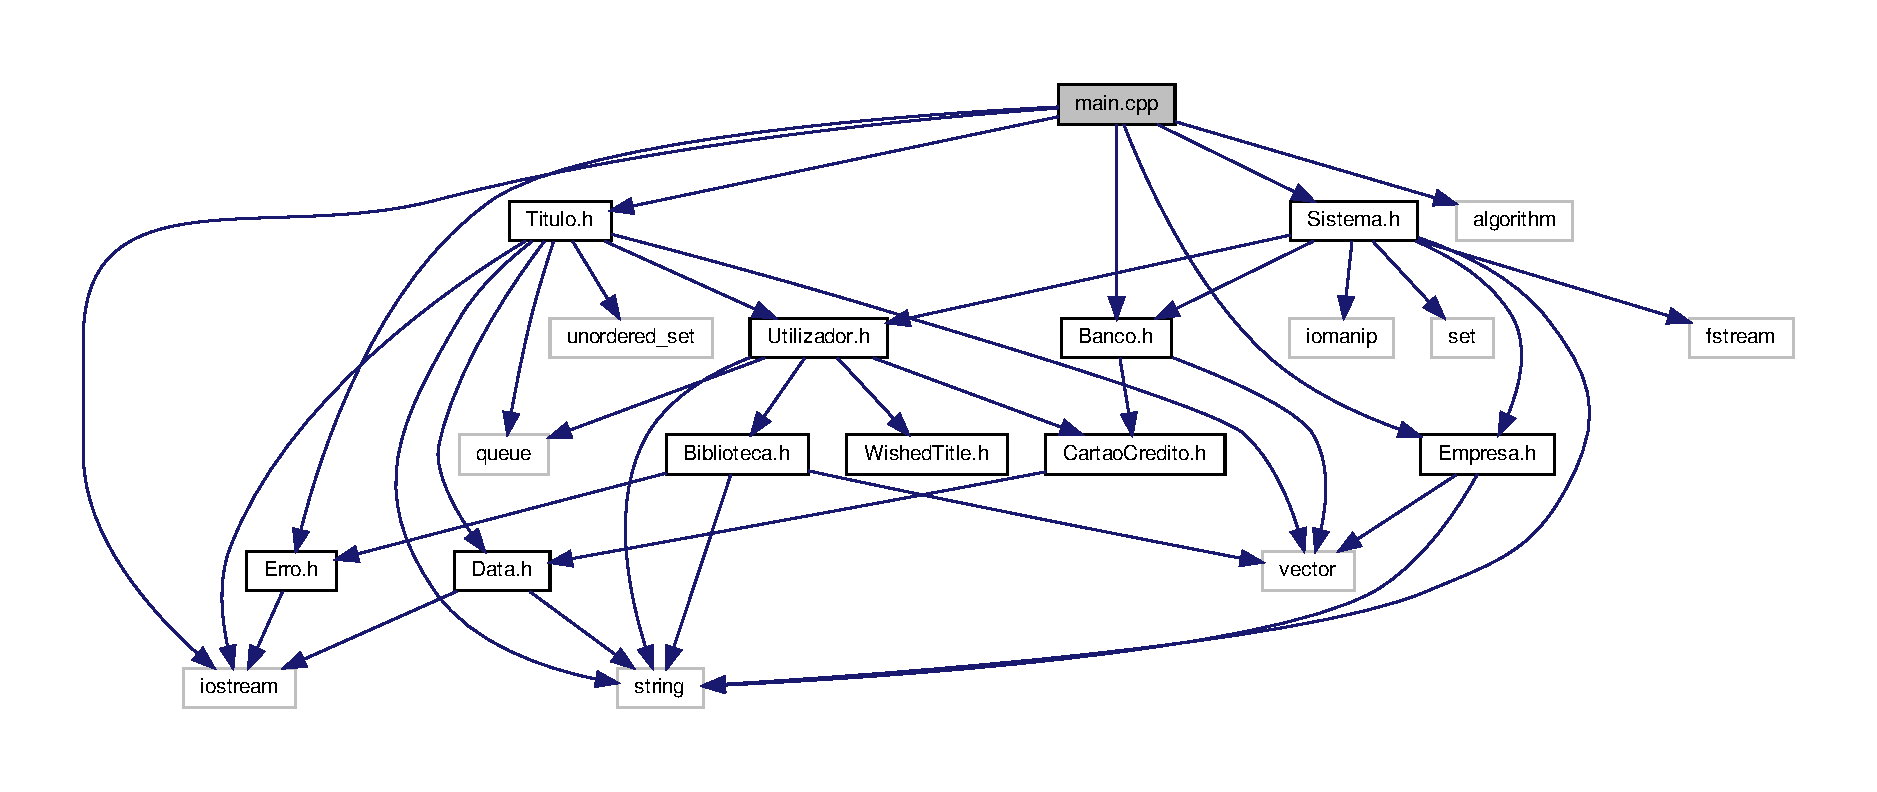
\includegraphics[width=350pt]{main_8cpp__incl}
\end{center}
\end{figure}
\subsection*{Functions}
\begin{DoxyCompactItemize}
\item 
int \hyperlink{main_8cpp_a69864162453f9299380c3c91be8fdca4}{get\+Option} (int min, int max)
\item 
void \hyperlink{main_8cpp_a89a9bf7f76b270a3a9fc783b4009586c}{print\+Welcome\+Menu} ()
\item 
void \hyperlink{main_8cpp_a575a2b817f03c17e7943087813687578}{print\+Display\+Empresas\+Menu} ()
\item 
void \hyperlink{main_8cpp_a9cdfd6b998ba8cfc497af7a303a6e330}{print\+Display\+Asleep\+Users\+Menu} ()
\item 
void \hyperlink{main_8cpp_af9dce1973196a5934ee5ec20ea417324}{print\+Main\+Menu} ()
\item 
void \hyperlink{main_8cpp_a3687e2ced7dee82b39fc1ed74674ecd5}{print\+Display\+Utilizadores\+Menu} ()
\item 
void \hyperlink{main_8cpp_a1b2cb3eb63cb3b95f68b994271b23f13}{print\+User\+Menu} ()
\item 
void \hyperlink{main_8cpp_a6afc9271571dfdc7288faf87e9616e7d}{print\+Display\+Titulos\+Menu} ()
\item 
void \hyperlink{main_8cpp_a874c5a99e7c57fa9c6bc09580292dab9}{adicionar\+Utilizador} (\hyperlink{classSistema}{Sistema} $\ast$sistema)
\item 
void \hyperlink{main_8cpp_afdd4f73eaf1ae01f9f045850fe275884}{ler\+Data} (std\+::string data)
\item 
void \hyperlink{main_8cpp_af223924a460aa7610e351d33b9105191}{adicionar\+Jogo} (\hyperlink{classSistema}{Sistema} $\ast$sistema, std\+::string nome\+Empresa)
\item 
bool \hyperlink{main_8cpp_a6c175a1424e435dba38c472eaf2f5535}{is\+\_\+digits} (const std\+::string \&str)
\item 
void \hyperlink{main_8cpp_ae1e120878470259b19387b335d21eb69}{adicionar\+Empresa} (\hyperlink{classSistema}{Sistema} $\ast$sistema)
\item 
void \hyperlink{main_8cpp_a633c2853177204cb3a7a8033e5b9497c}{display\+Utilizadores} (\hyperlink{classSistema}{Sistema} $\ast$sistema)
\item 
void \hyperlink{main_8cpp_aec6f563871c737f7e128ea66836a2be5}{ordena\+Jogos\+Utilizador} (\hyperlink{classSistema}{Sistema} $\ast$sistema, \hyperlink{classUtilizador}{Utilizador} $\ast$u)
\item 
void \hyperlink{main_8cpp_a5e58c15f905db107f320734a18f4e40d}{display\+Titulos} (\hyperlink{classSistema}{Sistema} $\ast$sistema)
\item 
void \hyperlink{main_8cpp_a3a9e67719857d943301b2926cd804e8c}{display\+Empresas} (\hyperlink{classSistema}{Sistema} $\ast$sistema)
\item 
void \hyperlink{main_8cpp_ae8e4ad4c7859f965d182b4bfb5e16abc}{display\+Asleep\+Users} (\hyperlink{classSistema}{Sistema} $\ast$sistema)
\item 
void \hyperlink{main_8cpp_af8f302c02e726f24c5f7ddea9cd7f17d}{escolhe\+Titulo} (\hyperlink{classSistema}{Sistema} $\ast$sistema, \hyperlink{classUtilizador}{Utilizador} $\ast$u)
\item 
void \hyperlink{main_8cpp_a11ccc3a4082cb5f294bc863d50fa803e}{adicona\+Wishlist} (\hyperlink{classSistema}{Sistema} $\ast$sistema, \hyperlink{classUtilizador}{Utilizador} $\ast$u)
\item 
void \hyperlink{main_8cpp_a01a46c12aa32213dc4babb7780904eba}{remover\+Wishlist} (\hyperlink{classSistema}{Sistema} $\ast$sistema, \hyperlink{classUtilizador}{Utilizador} $\ast$u)
\item 
void \hyperlink{main_8cpp_aeeed8d2818f5d3d47c30b792b064f1d8}{altera\+Interesse} (\hyperlink{classSistema}{Sistema} $\ast$sistema, \hyperlink{classUtilizador}{Utilizador} $\ast$u)
\item 
void \hyperlink{main_8cpp_aa59523879399e16bcfde4f06af6ad2ff}{escolhe\+Cc} (\hyperlink{classSistema}{Sistema} $\ast$sistema, \hyperlink{classUtilizador}{Utilizador} $\ast$u)
\item 
void \hyperlink{main_8cpp_aab039f6f4271b56e9ca2d1264b25f66a}{utilizador\+Joga} (\hyperlink{classSistema}{Sistema} $\ast$sistema, \hyperlink{classUtilizador}{Utilizador} $\ast$u)
\item 
void \hyperlink{main_8cpp_a28b549948b369d4db7a926ec0cfd6e77}{print\+Empresa\+Menu} ()
\item 
void \hyperlink{main_8cpp_a175192136cbe59d60bb80a1cd975fb68}{menu\+Empresa} (\hyperlink{classSistema}{Sistema} $\ast$sistema, \hyperlink{classEmpresa}{Empresa} $\ast$empresa)
\item 
void \hyperlink{main_8cpp_a41dd1ea1b95901e643be4af34f6dcfbf}{menu\+Utilizador} (\hyperlink{classSistema}{Sistema} $\ast$sistema, \hyperlink{classUtilizador}{Utilizador} $\ast$u)
\item 
void \hyperlink{main_8cpp_ab36c65bcfd56b6a29bee851e57462ad2}{pesquisar\+Utilizador} (\hyperlink{classSistema}{Sistema} $\ast$sistema)
\item 
void \hyperlink{main_8cpp_a84916567707f41d606bb5cbdd44d6c17}{pesquisar\+Jogo} (\hyperlink{classSistema}{Sistema} $\ast$sistema)
\item 
void \hyperlink{main_8cpp_ab5d3bc5e7f94dade3058f2afb385c8a4}{pesquisar\+Empresa} (\hyperlink{classSistema}{Sistema} $\ast$sistema)
\item 
void \hyperlink{main_8cpp_a3da8cb0d6e5160fb3cf923a352965ff4}{print\+Ranking\+Menu} ()
\item 
void \hyperlink{main_8cpp_a0932ac5f24cb3fdd2a58f8d5bbdc9507}{display\+Rankings} (\hyperlink{classSistema}{Sistema} $\ast$sistema)
\item 
int \hyperlink{main_8cpp_ae66f6b31b5ad750f1fe042a706a4e3d4}{main} ()
\end{DoxyCompactItemize}


\subsection{Function Documentation}
\mbox{\Hypertarget{main_8cpp_ae1e120878470259b19387b335d21eb69}\label{main_8cpp_ae1e120878470259b19387b335d21eb69}} 
\index{main.\+cpp@{main.\+cpp}!adicionar\+Empresa@{adicionar\+Empresa}}
\index{adicionar\+Empresa@{adicionar\+Empresa}!main.\+cpp@{main.\+cpp}}
\subsubsection{\texorpdfstring{adicionar\+Empresa()}{adicionarEmpresa()}}
{\footnotesize\ttfamily void adicionar\+Empresa (\begin{DoxyParamCaption}\item[{\hyperlink{classSistema}{Sistema} $\ast$}]{sistema }\end{DoxyParamCaption})}


\begin{DoxyCode}
356                                         \{
357     std::string nome;
358     std::string email;
359     std::string numeroTelemovel;
360     std::string nif;
361     std::cout << \textcolor{stringliteral}{"\(\backslash\)nNome da empresa: "};
362     getline(std::cin, nome);
363 
364     \textcolor{keywordflow}{while} (\textcolor{keyword}{true}) \{
365         \textcolor{keywordflow}{try} \{
366             sistema->\hyperlink{classSistema_ac120f4aecf81933be110233f8dbf74c6}{isValidEmail}(email);
367         \} \textcolor{keywordflow}{catch} (\hyperlink{classErro}{Erro} &e) \{
368             std::cout << e.\hyperlink{classErro_abfc1e9735b259d88bb97828a23164eb0}{getInfo}() << std::endl;
369             \textcolor{keywordflow}{continue};
370         \}
371         \textcolor{keywordflow}{break};
372     \}
373 
374     \textcolor{keywordflow}{while}(\textcolor{keyword}{true})\{
375         std::cout << \textcolor{stringliteral}{"\(\backslash\)nIntroduza o numero de telemovel: "};
376         getline(std::cin, numeroTelemovel);
377         \textcolor{keywordflow}{if}(\hyperlink{main_8cpp_a6c175a1424e435dba38c472eaf2f5535}{is\_digits}(numeroTelemovel) && numeroTelemovel.size()==9)\{
378             \textcolor{keywordflow}{break};
379         \}
380         \textcolor{keywordflow}{if}(numeroTelemovel.size()!=9)\{
381             std::cout << \textcolor{stringliteral}{"Introduza um numero com 9 digitos\(\backslash\)n"};
382         \}
383         \textcolor{keywordflow}{else} std::cout << \textcolor{stringliteral}{"O numero de telemovel so pode ter algarismos"};
384     \}
385 
386     \textcolor{keywordflow}{while}(\textcolor{keyword}{true})\{
387         std::cout << \textcolor{stringliteral}{"Introduza o NIF: "};
388         getline(std::cin, nif);
389         \textcolor{keywordflow}{if}(\hyperlink{main_8cpp_a6c175a1424e435dba38c472eaf2f5535}{is\_digits}(nif) && nif.size()==9)\{
390             \textcolor{keywordflow}{break};
391         \}
392         \textcolor{keywordflow}{if}(nif.size()!=9)\{
393             std::cout << \textcolor{stringliteral}{"Introduza um NIF com 9 digitos\(\backslash\)n"};
394         \}
395         \textcolor{keywordflow}{else} std::cout << \textcolor{stringliteral}{"O NIF so pode ter algarismos"};
396     \}
397 
398     \hyperlink{classEmpresa}{Empresa} *empresa= \textcolor{keyword}{new} \hyperlink{classEmpresa}{Empresa}(nome,email,numeroTelemovel,nif);
399     \textcolor{keywordflow}{try}\{
400         sistema->\hyperlink{classSistema_a41eddc54d36ac140608dd259c085ba88}{adicionaEmpresa}(empresa);
401     \}
402     \textcolor{keywordflow}{catch}(\hyperlink{classEmpresaJaAdicionada}{EmpresaJaAdicionada} &e)\{
403         std::cout << \textcolor{stringliteral}{"\(\backslash\)n"} << e.\hyperlink{classErro_abfc1e9735b259d88bb97828a23164eb0}{getInfo}();
404     \}
405 \}
\end{DoxyCode}
Here is the call graph for this function\+:
\nopagebreak
\begin{figure}[H]
\begin{center}
\leavevmode
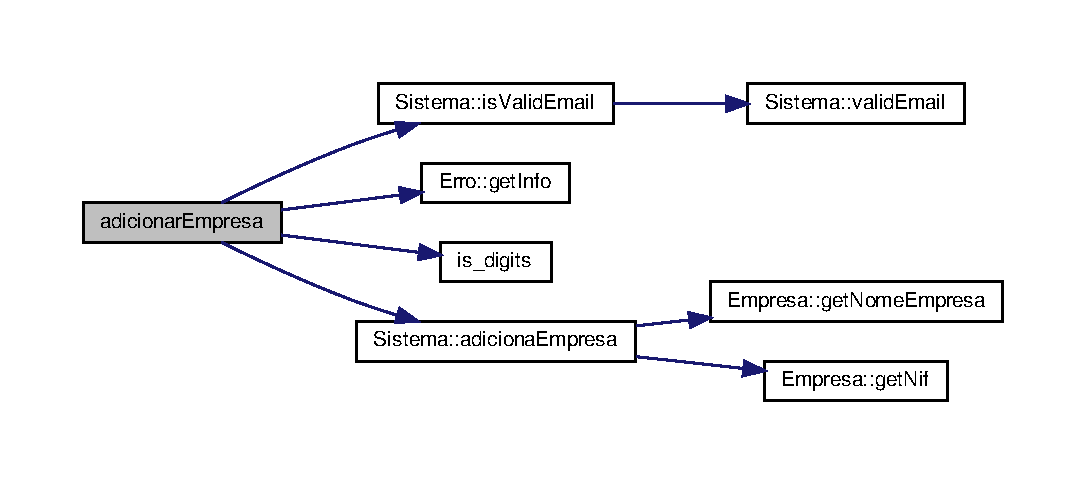
\includegraphics[width=350pt]{main_8cpp_ae1e120878470259b19387b335d21eb69_cgraph}
\end{center}
\end{figure}
Here is the caller graph for this function\+:
\nopagebreak
\begin{figure}[H]
\begin{center}
\leavevmode
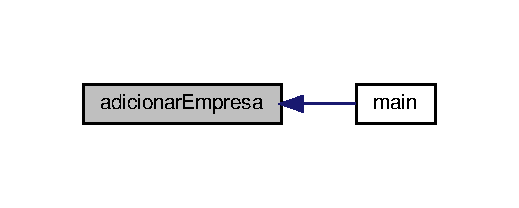
\includegraphics[width=249pt]{main_8cpp_ae1e120878470259b19387b335d21eb69_icgraph}
\end{center}
\end{figure}
\mbox{\Hypertarget{main_8cpp_af223924a460aa7610e351d33b9105191}\label{main_8cpp_af223924a460aa7610e351d33b9105191}} 
\index{main.\+cpp@{main.\+cpp}!adicionar\+Jogo@{adicionar\+Jogo}}
\index{adicionar\+Jogo@{adicionar\+Jogo}!main.\+cpp@{main.\+cpp}}
\subsubsection{\texorpdfstring{adicionar\+Jogo()}{adicionarJogo()}}
{\footnotesize\ttfamily void adicionar\+Jogo (\begin{DoxyParamCaption}\item[{\hyperlink{classSistema}{Sistema} $\ast$}]{sistema,  }\item[{std\+::string}]{nome\+Empresa }\end{DoxyParamCaption})}


\begin{DoxyCode}
231                                                              \{
232     std::cout << \textcolor{stringliteral}{"Adicionar um titulo \(\backslash\)n"};
233 
234     std::cout << std::endl << \textcolor{stringliteral}{"Tipo de Titulo (Home, Online): "};
235     std::string tipo;
236     getline(std::cin, tipo);
237     \textcolor{keywordflow}{while} (tipo != \textcolor{stringliteral}{"Home"} && tipo != \textcolor{stringliteral}{"Online"}) \{
238         std::cout << \textcolor{stringliteral}{"Introduza um tipo de titulo valido"} << std::endl;
239         getline(std::cin, tipo);
240     \}
241 
242     std::cout << std::endl << \textcolor{stringliteral}{"Nome do titulo: "};
243     std::string nome;
244     getline(std::cin, nome);
245 
246     std::string data;
247     \textcolor{keywordflow}{while} (\textcolor{keyword}{true}) \{
248         std::cout << \textcolor{stringliteral}{"\(\backslash\)nData de lancamento (Formato DD/MM/AAAA): "};
249         getline(std::cin, data);
250         \textcolor{keywordflow}{try} \{
251             \hyperlink{main_8cpp_afdd4f73eaf1ae01f9f045850fe275884}{lerData}(data);
252         \} \textcolor{keywordflow}{catch} (\hyperlink{classDataInvalida}{DataInvalida} &e) \{
253             std::cout << \textcolor{stringliteral}{"\(\backslash\)n"} << e.\hyperlink{classErro_abfc1e9735b259d88bb97828a23164eb0}{getInfo}() << std::endl
254                     << \textcolor{stringliteral}{"Introduza novamente"} << std::endl;
255             \textcolor{keywordflow}{continue};
256         \}
257         \textcolor{keywordflow}{break};
258     \}
259 
260     std::cout << std::endl << \textcolor{stringliteral}{"Preco do titulo: "};
261     \textcolor{keywordtype}{float} preco;
262     std::cin >> preco;
263     \textcolor{comment}{// Verificar se foi introduzido um numero}
264     \textcolor{keywordflow}{while} (std::cin.fail() || std::cin.eof() || preco <= 0) \{
265         std::cin.clear();
266         std::cin.ignore(1000, \textcolor{charliteral}{'\(\backslash\)n'});
267         std::cout << \textcolor{stringliteral}{"Preco Invalido! Introduza novamente."} << std::endl;
268         std::cout << std::endl << \textcolor{stringliteral}{"Preco do titulo: "};
269         std::cin >> preco;
270     \}
271 
272     \textcolor{comment}{// Limpar a stream mesmo que n�o tenha ocorrido qualquer erro, para garantir que est� sempre limpa e
       vazia}
273     std::cin.ignore(1000, \textcolor{charliteral}{'\(\backslash\)n'});
274 
275     \textcolor{keywordtype}{int} idadeMinima;
276     std::cout << std::endl << \textcolor{stringliteral}{"Idade minima: "};
277     std::cin >> idadeMinima;
278     \textcolor{comment}{// Verificar se foi introduzido um numero}
279     \textcolor{keywordflow}{while} (std::cin.fail() || std::cin.eof() || idadeMinima <= 0) \{
280         std::cin.clear();
281         std::cin.ignore(1000, \textcolor{charliteral}{'\(\backslash\)n'});
282         std::cout << \textcolor{stringliteral}{"Idade invalida! Introduza novamente."} << std::endl;
283         std::cout << std::endl << \textcolor{stringliteral}{"Idade Minima: "};
284         std::cin >> idadeMinima;
285     \}
286     std::cin.ignore(1000, \textcolor{charliteral}{'\(\backslash\)n'});
287 
288     std::string plataforma;
289     std::cout << std::endl << \textcolor{stringliteral}{"Plataforma: "};
290     getline(std::cin, plataforma);
291 
292     std::vector<std::string> generos;
293     std::string genero;
294     std::cout << std::endl
295             << \textcolor{stringliteral}{"Generos (Introduza um genero de cada vez e introduza '.' quando terminar. Necessario pelo
       menos um genero!): "};
296     \textcolor{keywordflow}{while} (genero[0] != \textcolor{charliteral}{'.'} || (!generos.size())) \{
297         getline(std::cin, genero);
298         \textcolor{keywordflow}{if} (genero[0] != \textcolor{charliteral}{'.'}) \{
299             generos.push\_back(genero);
300         \}
301     \}
302 
303     \textcolor{keywordflow}{if} (tipo == \textcolor{stringliteral}{"Home"}) \{
304         \hyperlink{classHome}{Home} *home = \textcolor{keyword}{new} \hyperlink{classHome}{Home}(nome, idadeMinima, plataforma, preco, generos,
305                 nomeEmpresa, \hyperlink{classData}{Data}(data), 0, 0);
306         \textcolor{keywordflow}{try} \{
307             sistema->\hyperlink{classSistema_a1136080a3cf835831bf94908d419ae42}{addTitulo}(home,nomeEmpresa);
308         \} \textcolor{keywordflow}{catch} (\hyperlink{classTituloJaAdicionado}{TituloJaAdicionado} &e) \{
309             std::cout << e.\hyperlink{classErro_abfc1e9735b259d88bb97828a23164eb0}{getInfo}() << std::endl;
310         \}
311 
312     \} \textcolor{keywordflow}{else} \textcolor{keywordflow}{if} (tipo == \textcolor{stringliteral}{"Online"}) \{
313         std::cout << std::endl << \textcolor{stringliteral}{"Tipo de subscricao ( Variavel ou Fixa ): "};
314         std::string tipoSubs;
315         getline(std::cin, tipoSubs);
316         \textcolor{keywordflow}{while} (tipoSubs != \textcolor{stringliteral}{"Variavel"} && tipoSubs != \textcolor{stringliteral}{"Fixa"}) \{
317             std::cout << \textcolor{stringliteral}{"Introduza um tipo de subscricao valida"} << std::endl;
318             getline(std::cin, tipoSubs);
319         \}
320         \textcolor{keywordtype}{bool} tipoSubscricao;
321         \textcolor{keywordflow}{if} (tipoSubs == \textcolor{stringliteral}{"Variavel"}) \{
322             tipoSubscricao = \textcolor{keyword}{false};
323         \} \textcolor{keywordflow}{else}
324             tipoSubscricao = \textcolor{keyword}{true};
325         \textcolor{keywordtype}{float} precoSubscricao;
326         std::cout << std::endl << \textcolor{stringliteral}{"Preco de Subscricao: "};
327         std::cin >> precoSubscricao;
328         \textcolor{comment}{// Verificar se foi introduzido um numero}
329         \textcolor{keywordflow}{while} (std::cin.fail() || std::cin.eof() || precoSubscricao <= 0) \{
330             std::cin.clear();
331             std::cin.ignore(1000, \textcolor{charliteral}{'\(\backslash\)n'});
332             std::cout << \textcolor{stringliteral}{"Preco Invalido! Introduza novamente."} << std::endl;
333             std::cout << std::endl << \textcolor{stringliteral}{"Preco de Subscricao: "};
334             std::cin >> precoSubscricao;
335         \}
336 
337         std::cin.ignore(1000, \textcolor{charliteral}{'\(\backslash\)n'});
338         \hyperlink{classOnline}{Online} *online = \textcolor{keyword}{new} \hyperlink{classOnline}{Online}(nome, idadeMinima, plataforma, preco,
339                 generos, nomeEmpresa, \hyperlink{classData}{Data}(data), 0, 0, tipoSubscricao, precoSubscricao);
340         \textcolor{keywordflow}{try} \{
341             sistema->\hyperlink{classSistema_a1136080a3cf835831bf94908d419ae42}{addTitulo}(online,nomeEmpresa);
342         \} \textcolor{keywordflow}{catch} (\hyperlink{classTituloJaAdicionado}{TituloJaAdicionado} &e) \{
343             std::cout << \textcolor{stringliteral}{"\(\backslash\)n"} << e.\hyperlink{classErro_abfc1e9735b259d88bb97828a23164eb0}{getInfo}();
344         \}
345     \}
346 
347     std::cout << \textcolor{stringliteral}{"O titulo "} << nome << \textcolor{stringliteral}{" adicionado com sucesso!"} << std::endl
348             << std::endl;
349 \}
\end{DoxyCode}
Here is the call graph for this function\+:
\nopagebreak
\begin{figure}[H]
\begin{center}
\leavevmode
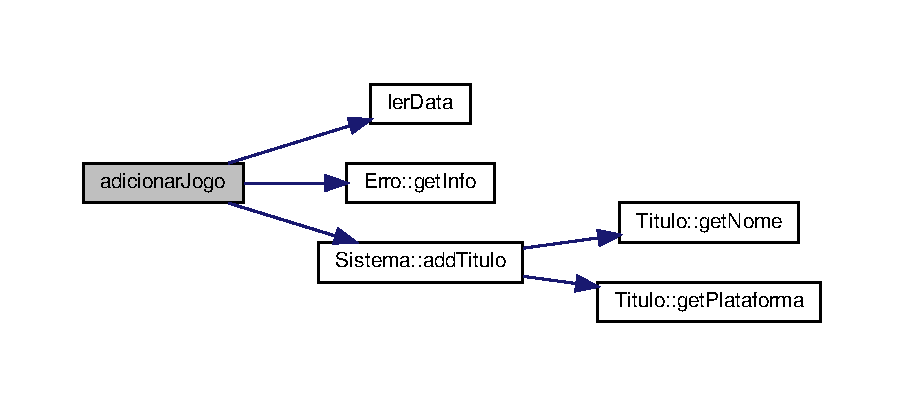
\includegraphics[width=350pt]{main_8cpp_af223924a460aa7610e351d33b9105191_cgraph}
\end{center}
\end{figure}
Here is the caller graph for this function\+:
\nopagebreak
\begin{figure}[H]
\begin{center}
\leavevmode
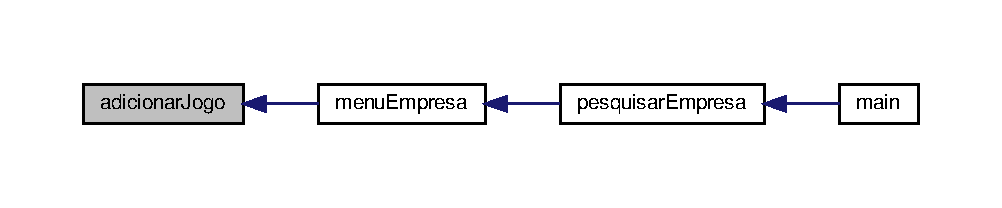
\includegraphics[width=350pt]{main_8cpp_af223924a460aa7610e351d33b9105191_icgraph}
\end{center}
\end{figure}
\mbox{\Hypertarget{main_8cpp_a874c5a99e7c57fa9c6bc09580292dab9}\label{main_8cpp_a874c5a99e7c57fa9c6bc09580292dab9}} 
\index{main.\+cpp@{main.\+cpp}!adicionar\+Utilizador@{adicionar\+Utilizador}}
\index{adicionar\+Utilizador@{adicionar\+Utilizador}!main.\+cpp@{main.\+cpp}}
\subsubsection{\texorpdfstring{adicionar\+Utilizador()}{adicionarUtilizador()}}
{\footnotesize\ttfamily void adicionar\+Utilizador (\begin{DoxyParamCaption}\item[{\hyperlink{classSistema}{Sistema} $\ast$}]{sistema }\end{DoxyParamCaption})}


\begin{DoxyCode}
136                                             \{
137 
138     std::string nome;
139     std::string email;
140     std::string idade;
141     std::string morada;
142     std::cout << \textcolor{stringliteral}{"A criar utilizador...  \(\backslash\)n"};
143     std::cout << \textcolor{stringliteral}{"Insere um nome: "};
144     getline(std::cin, nome);
145 
146     \textcolor{keywordflow}{while} (\textcolor{keyword}{true}) \{
147         \textcolor{keywordflow}{try} \{
148             sistema->\hyperlink{classSistema_ac120f4aecf81933be110233f8dbf74c6}{isValidEmail}(email);
149         \} \textcolor{keywordflow}{catch} (\hyperlink{classErro}{Erro} &e) \{
150             std::cout << e.\hyperlink{classErro_abfc1e9735b259d88bb97828a23164eb0}{getInfo}() << std::endl;
151             \textcolor{keywordflow}{continue};
152         \}
153         \textcolor{keywordflow}{break};
154     \}
155 
156     std::cout << \textcolor{stringliteral}{"Insere a tua idade: "};
157     getline(std::cin, idade);
158     std::cout << \textcolor{stringliteral}{"Insere a tua morada: "};
159     getline(std::cin, morada);
160 
161     \hyperlink{classUtilizador}{Utilizador} *u = \textcolor{keyword}{new} \hyperlink{classUtilizador}{Utilizador}(nome, email, std::stoul(idade, NULL, 0), morada);
162     sistema->\hyperlink{classSistema_a51beac85364444837cd4cdff0080bad5}{adicionaUtilizador}(u);
163 
164     std::cout << \textcolor{stringliteral}{"Utilizador guardado com sucesso!"} << std::endl << std::endl;
165     \textcolor{keywordflow}{return};
166 \}
\end{DoxyCode}
Here is the call graph for this function\+:
\nopagebreak
\begin{figure}[H]
\begin{center}
\leavevmode
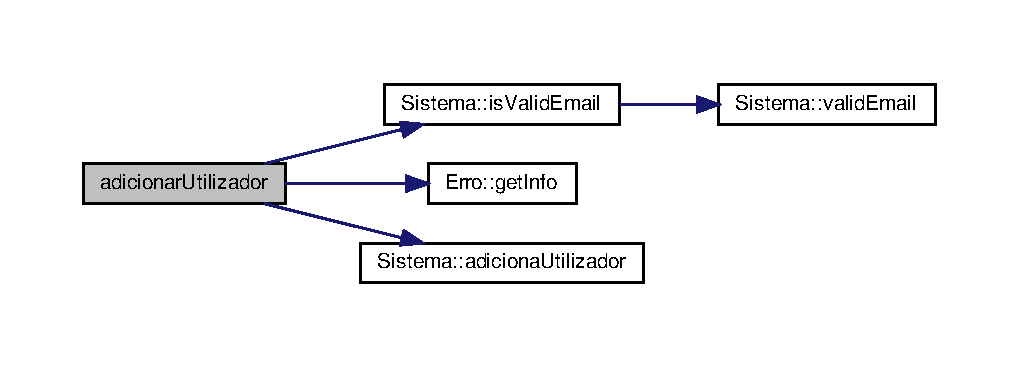
\includegraphics[width=350pt]{main_8cpp_a874c5a99e7c57fa9c6bc09580292dab9_cgraph}
\end{center}
\end{figure}
Here is the caller graph for this function\+:
\nopagebreak
\begin{figure}[H]
\begin{center}
\leavevmode
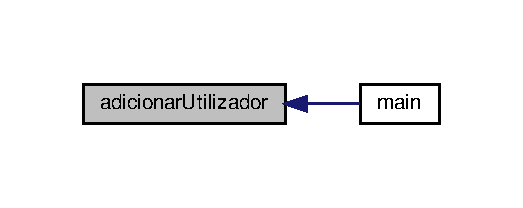
\includegraphics[width=251pt]{main_8cpp_a874c5a99e7c57fa9c6bc09580292dab9_icgraph}
\end{center}
\end{figure}
\mbox{\Hypertarget{main_8cpp_a11ccc3a4082cb5f294bc863d50fa803e}\label{main_8cpp_a11ccc3a4082cb5f294bc863d50fa803e}} 
\index{main.\+cpp@{main.\+cpp}!adicona\+Wishlist@{adicona\+Wishlist}}
\index{adicona\+Wishlist@{adicona\+Wishlist}!main.\+cpp@{main.\+cpp}}
\subsubsection{\texorpdfstring{adicona\+Wishlist()}{adiconaWishlist()}}
{\footnotesize\ttfamily void adicona\+Wishlist (\begin{DoxyParamCaption}\item[{\hyperlink{classSistema}{Sistema} $\ast$}]{sistema,  }\item[{\hyperlink{classUtilizador}{Utilizador} $\ast$}]{u }\end{DoxyParamCaption})}


\begin{DoxyCode}
621                                                      \{
622     std::string titulo;
623     std::string plataforma;
624     std::string s;
625 
626     \textcolor{keywordflow}{while} (\textcolor{keyword}{true}) \{
627         std::cout << \textcolor{stringliteral}{"Insira o nome do titulo"} << std::endl;
628         getline(std::cin, titulo);
629         std::cout << \textcolor{stringliteral}{"Insira a plataforma"} << std::endl;
630         getline(std::cin, plataforma);
631 
632         \textcolor{keywordflow}{try} \{
633             \hyperlink{classTitulo}{Titulo} * t = sistema->\hyperlink{classSistema_a0fb81a4685bb24024295c89d22d6d719}{pesquisaJogo}(titulo, plataforma);
634 
635             \textcolor{keywordtype}{unsigned} \textcolor{keywordtype}{int} interesse;
636             std::cout << std::endl << \textcolor{stringliteral}{"Interesse (1 - 10) "};
637             std::cin >> interesse;
638             \textcolor{comment}{// Verificar se foi introduzido um numero}
639             \textcolor{keywordflow}{while} (std::cin.fail() || std::cin.eof() || interesse <= 0 || interesse > 10) \{
640                 std::cin.clear();
641                 std::cin.ignore(1000, \textcolor{charliteral}{'\(\backslash\)n'});
642                 std::cout << \textcolor{stringliteral}{"Interesse invalido! Introduza novamente."} << std::endl;
643                 std::cout << std::endl << \textcolor{stringliteral}{"Interesse (1 - 10): "};
644                 std::cin >> interesse;
645             \}
646             std::cin.ignore(1000, \textcolor{charliteral}{'\(\backslash\)n'});
647             u->\hyperlink{classUtilizador_a45ee0a8d988adbd537e2506d80f96cfb}{adicionaWishList}(t,interesse);
648         \} \textcolor{keywordflow}{catch} (\hyperlink{classErro}{Erro} &e) \{
649             std::cout << e.\hyperlink{classErro_abfc1e9735b259d88bb97828a23164eb0}{getInfo}() << std::endl;
650             std::cout
651                     << \textcolor{stringliteral}{"Deseja desistir da procura('s' para sair/ outro para continuar)?"}
652                     << std::endl;
653             getline(std::cin, s);
654             \textcolor{keywordflow}{if} (s == \textcolor{stringliteral}{"s"})
655                 \textcolor{keywordflow}{return};
656 
657             \textcolor{keywordflow}{continue};
658         \}
659         std::cout << \textcolor{stringliteral}{"Jogo inserido com sucesso!"} << std::endl;
660         \textcolor{keywordflow}{break};
661     \}
662 \}
\end{DoxyCode}
Here is the call graph for this function\+:
\nopagebreak
\begin{figure}[H]
\begin{center}
\leavevmode
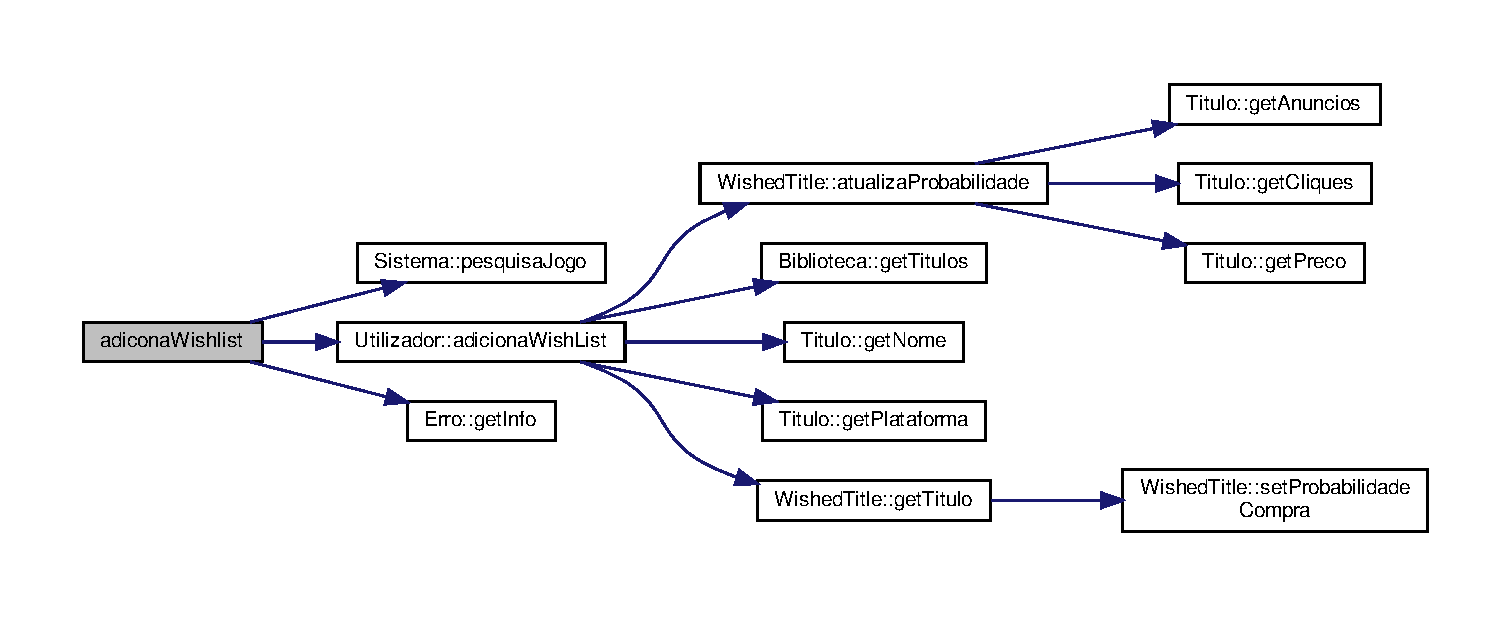
\includegraphics[width=350pt]{main_8cpp_a11ccc3a4082cb5f294bc863d50fa803e_cgraph}
\end{center}
\end{figure}
Here is the caller graph for this function\+:
\nopagebreak
\begin{figure}[H]
\begin{center}
\leavevmode
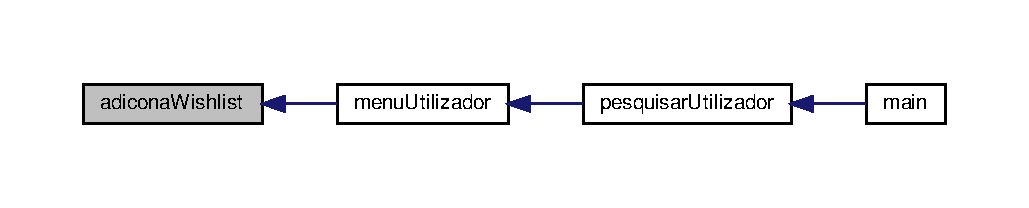
\includegraphics[width=350pt]{main_8cpp_a11ccc3a4082cb5f294bc863d50fa803e_icgraph}
\end{center}
\end{figure}
\mbox{\Hypertarget{main_8cpp_aeeed8d2818f5d3d47c30b792b064f1d8}\label{main_8cpp_aeeed8d2818f5d3d47c30b792b064f1d8}} 
\index{main.\+cpp@{main.\+cpp}!altera\+Interesse@{altera\+Interesse}}
\index{altera\+Interesse@{altera\+Interesse}!main.\+cpp@{main.\+cpp}}
\subsubsection{\texorpdfstring{altera\+Interesse()}{alteraInteresse()}}
{\footnotesize\ttfamily void altera\+Interesse (\begin{DoxyParamCaption}\item[{\hyperlink{classSistema}{Sistema} $\ast$}]{sistema,  }\item[{\hyperlink{classUtilizador}{Utilizador} $\ast$}]{u }\end{DoxyParamCaption})}


\begin{DoxyCode}
706                                                      \{
707     std::string titulo;
708     std::string plataforma;
709     std::string s;
710 
711     \textcolor{keywordflow}{while} (\textcolor{keyword}{true}) \{
712         std::cout << \textcolor{stringliteral}{"Insira o nome do titulo"} << std::endl;
713         getline(std::cin, titulo);
714         std::cout << \textcolor{stringliteral}{"Insira a plataforma"} << std::endl;
715         getline(std::cin, plataforma);
716 
717         \textcolor{keywordflow}{try} \{
718             \hyperlink{classTitulo}{Titulo} * t = sistema->\hyperlink{classSistema_a0fb81a4685bb24024295c89d22d6d719}{pesquisaJogo}(titulo, plataforma);
719             \textcolor{keywordtype}{unsigned} \textcolor{keywordtype}{int} interesse;
720             std::cout << std::endl << \textcolor{stringliteral}{"Interesse (1 - 10) "};
721             std::cin >> interesse;
722             \textcolor{comment}{// Verificar se foi introduzido um numero}
723             \textcolor{keywordflow}{while} (std::cin.fail() || std::cin.eof() || interesse <= 0 || interesse > 10) \{
724                 std::cin.clear();
725                 std::cin.ignore(1000, \textcolor{charliteral}{'\(\backslash\)n'});
726                 std::cout << \textcolor{stringliteral}{"Interesse invalido! Introduza novamente."} << std::endl;
727                 std::cout << std::endl << \textcolor{stringliteral}{"Interesse (1 - 10): "};
728                 std::cin >> interesse;
729             \}
730             std::cin.ignore(1000, \textcolor{charliteral}{'\(\backslash\)n'});
731             u->\hyperlink{classUtilizador_a4617169b0764e48f8b95d4d8aa12bf19}{atualizaInteresse}(t,interesse);
732         \} \textcolor{keywordflow}{catch} (\hyperlink{classErro}{Erro} &e) \{
733             std::cout << e.\hyperlink{classErro_abfc1e9735b259d88bb97828a23164eb0}{getInfo}() << std::endl;
734             std::cout
735                     << \textcolor{stringliteral}{"Deseja desistir da procura('s' para sair/ outro para continuar)?"}
736                     << std::endl;
737             getline(std::cin, s);
738             \textcolor{keywordflow}{if} (s == \textcolor{stringliteral}{"s"})
739                 \textcolor{keywordflow}{return};
740 
741             \textcolor{keywordflow}{continue};
742         \}
743         std::cout << \textcolor{stringliteral}{"Interesse alterado com sucesso!"} << std::endl;
744         \textcolor{keywordflow}{break};
745     \}
746 \}
\end{DoxyCode}
Here is the call graph for this function\+:
\nopagebreak
\begin{figure}[H]
\begin{center}
\leavevmode
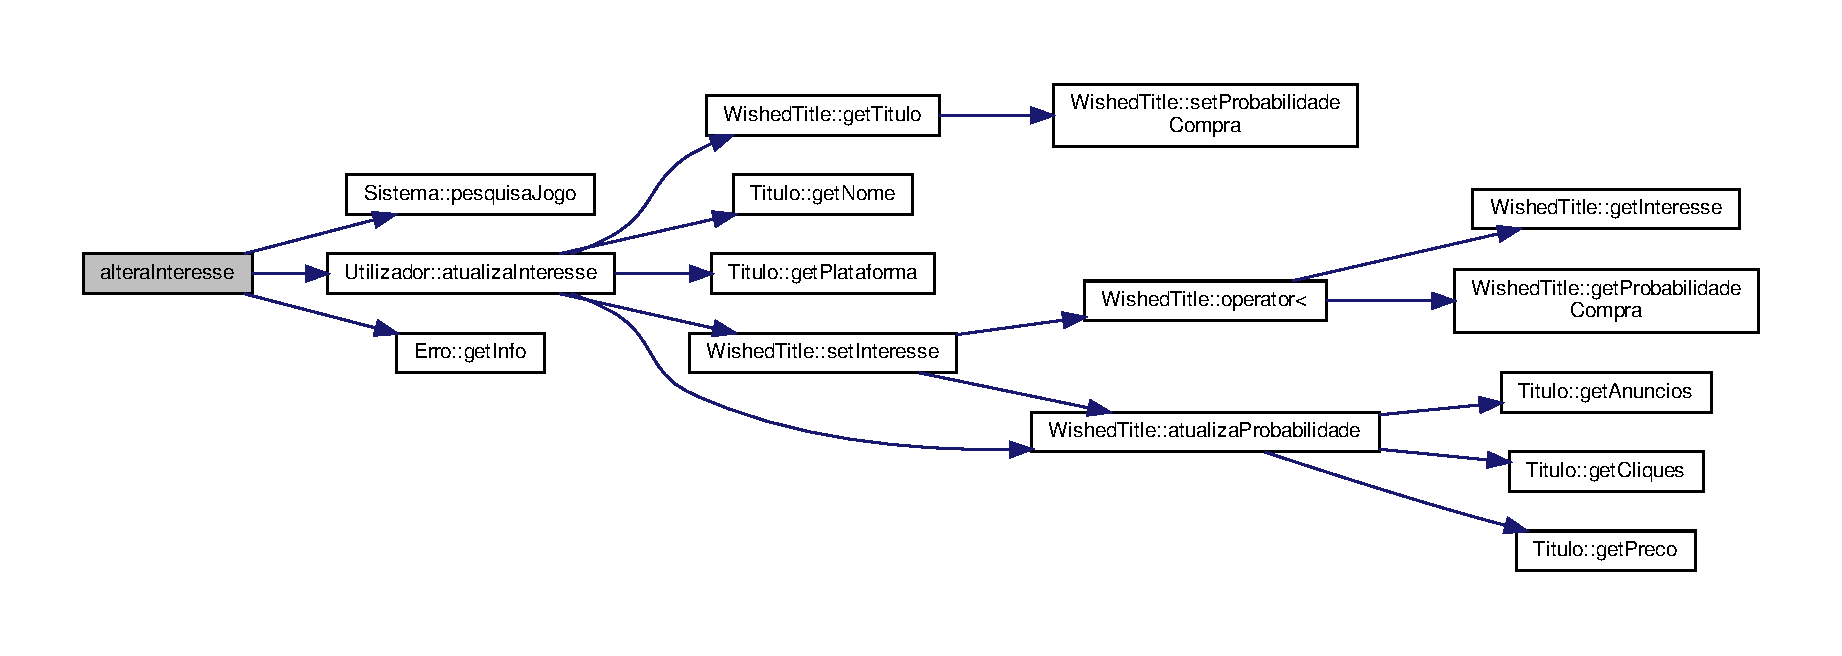
\includegraphics[width=350pt]{main_8cpp_aeeed8d2818f5d3d47c30b792b064f1d8_cgraph}
\end{center}
\end{figure}
Here is the caller graph for this function\+:
\nopagebreak
\begin{figure}[H]
\begin{center}
\leavevmode
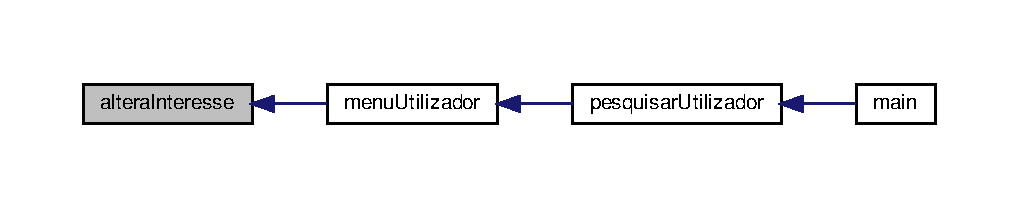
\includegraphics[width=350pt]{main_8cpp_aeeed8d2818f5d3d47c30b792b064f1d8_icgraph}
\end{center}
\end{figure}
\mbox{\Hypertarget{main_8cpp_ae8e4ad4c7859f965d182b4bfb5e16abc}\label{main_8cpp_ae8e4ad4c7859f965d182b4bfb5e16abc}} 
\index{main.\+cpp@{main.\+cpp}!display\+Asleep\+Users@{display\+Asleep\+Users}}
\index{display\+Asleep\+Users@{display\+Asleep\+Users}!main.\+cpp@{main.\+cpp}}
\subsubsection{\texorpdfstring{display\+Asleep\+Users()}{displayAsleepUsers()}}
{\footnotesize\ttfamily void display\+Asleep\+Users (\begin{DoxyParamCaption}\item[{\hyperlink{classSistema}{Sistema} $\ast$}]{sistema }\end{DoxyParamCaption})}


\begin{DoxyCode}
541                                          \{
542     \textcolor{keywordtype}{int} opt;
543 
544     \textcolor{comment}{// Perguntar ao utilizador o que quer fazer ate este indicar que deseja sair}
545     \textcolor{keywordflow}{while} (\textcolor{keyword}{true}) \{
546         \hyperlink{main_8cpp_a9cdfd6b998ba8cfc497af7a303a6e330}{printDisplayAsleepUsersMenu}();
547 
548         \textcolor{comment}{// Pedir opcao ao utilizador e verificar se nao houve erro de input}
549         \textcolor{keywordflow}{try} \{
550             opt = \hyperlink{main_8cpp_a69864162453f9299380c3c91be8fdca4}{getOption}(1, 5);
551         \} \textcolor{keywordflow}{catch} (\hyperlink{classInputInvalido}{InputInvalido} &e) \{
552             std::cout << \textcolor{stringliteral}{"\(\backslash\)n"} << e.\hyperlink{classErro_abfc1e9735b259d88bb97828a23164eb0}{getInfo}();
553             \textcolor{keywordflow}{continue};   \textcolor{comment}{// Ir para o proximo loop , pedir nova opcao}
554         \}
555 
556         \textcolor{keywordflow}{if} (opt == 1)
557             sistema->\hyperlink{classSistema_a6f73ddef363e2bc3e1c36dcb0d6d6152}{displayAsleepUsers}(\textcolor{stringliteral}{""});
558         \textcolor{keywordflow}{else} \textcolor{keywordflow}{if} (opt == 2)
559             sistema->\hyperlink{classSistema_a6f73ddef363e2bc3e1c36dcb0d6d6152}{displayAsleepUsers}(\textcolor{stringliteral}{"plataforma"});
560         \textcolor{keywordflow}{else} \textcolor{keywordflow}{if}(opt==3)
561             sistema->\hyperlink{classSistema_a6f73ddef363e2bc3e1c36dcb0d6d6152}{displayAsleepUsers}(\textcolor{stringliteral}{"titulo"});
562         \textcolor{keywordflow}{else} \textcolor{keywordflow}{if} (opt == 4)
563             sistema->\hyperlink{classSistema_a6f73ddef363e2bc3e1c36dcb0d6d6152}{displayAsleepUsers}(\textcolor{stringliteral}{"genero"});
564         \textcolor{keywordflow}{else} \textcolor{keywordflow}{if} (opt == 5)
565             \textcolor{keywordflow}{return};
566     \}
567 \}
\end{DoxyCode}
Here is the call graph for this function\+:
\nopagebreak
\begin{figure}[H]
\begin{center}
\leavevmode
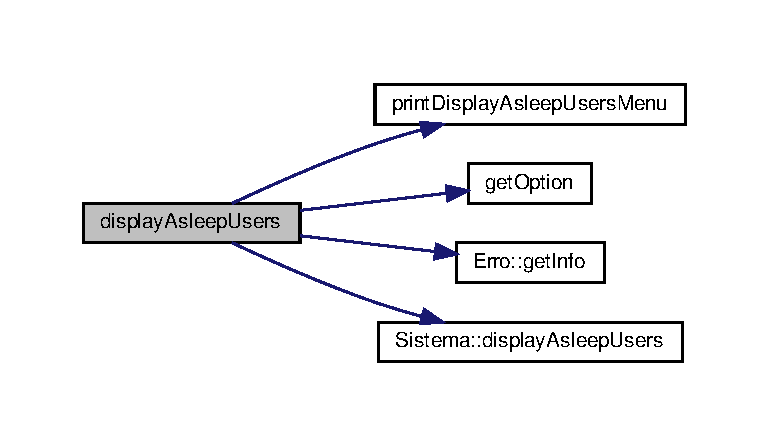
\includegraphics[width=350pt]{main_8cpp_ae8e4ad4c7859f965d182b4bfb5e16abc_cgraph}
\end{center}
\end{figure}
Here is the caller graph for this function\+:
\nopagebreak
\begin{figure}[H]
\begin{center}
\leavevmode
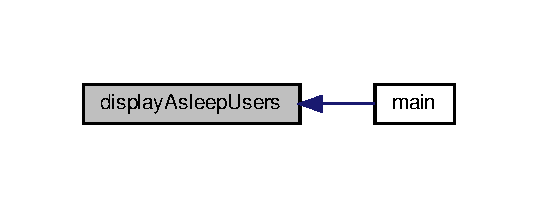
\includegraphics[width=258pt]{main_8cpp_ae8e4ad4c7859f965d182b4bfb5e16abc_icgraph}
\end{center}
\end{figure}
\mbox{\Hypertarget{main_8cpp_a3a9e67719857d943301b2926cd804e8c}\label{main_8cpp_a3a9e67719857d943301b2926cd804e8c}} 
\index{main.\+cpp@{main.\+cpp}!display\+Empresas@{display\+Empresas}}
\index{display\+Empresas@{display\+Empresas}!main.\+cpp@{main.\+cpp}}
\subsubsection{\texorpdfstring{display\+Empresas()}{displayEmpresas()}}
{\footnotesize\ttfamily void display\+Empresas (\begin{DoxyParamCaption}\item[{\hyperlink{classSistema}{Sistema} $\ast$}]{sistema }\end{DoxyParamCaption})}


\begin{DoxyCode}
513                                        \{
514     \textcolor{keywordtype}{int} opt;
515 
516     \textcolor{comment}{// Perguntar ao utilizador o que quer fazer ate este indicar que deseja sair}
517     \textcolor{keywordflow}{while} (\textcolor{keyword}{true}) \{
518         \hyperlink{main_8cpp_a575a2b817f03c17e7943087813687578}{printDisplayEmpresasMenu}();
519 
520         \textcolor{comment}{// Pedir opcao ao utilizador e verificar se nao houve erro de input}
521         \textcolor{keywordflow}{try} \{
522             opt = \hyperlink{main_8cpp_a69864162453f9299380c3c91be8fdca4}{getOption}(1, 5);
523         \} \textcolor{keywordflow}{catch} (\hyperlink{classInputInvalido}{InputInvalido} &e) \{
524             std::cout << \textcolor{stringliteral}{"\(\backslash\)n"} << e.\hyperlink{classErro_abfc1e9735b259d88bb97828a23164eb0}{getInfo}();
525             \textcolor{keywordflow}{continue};   \textcolor{comment}{// Ir para o proximo loop , pedir nova opcao}
526         \}
527 
528         \textcolor{keywordflow}{if} (opt == 1)
529             sistema->\hyperlink{classSistema_a4380aacc310d051a753138477d8e777f}{displayEmpresas}(\textcolor{stringliteral}{""});
530         \textcolor{keywordflow}{else} \textcolor{keywordflow}{if} (opt == 2)
531             sistema->\hyperlink{classSistema_a4380aacc310d051a753138477d8e777f}{displayEmpresas}(\textcolor{stringliteral}{"plataforma"});
532         \textcolor{keywordflow}{else} \textcolor{keywordflow}{if}(opt==3)
533             sistema->\hyperlink{classSistema_a4380aacc310d051a753138477d8e777f}{displayEmpresas}(\textcolor{stringliteral}{"numero"});
534         \textcolor{keywordflow}{else} \textcolor{keywordflow}{if} (opt == 4)
535             sistema->\hyperlink{classSistema_a4380aacc310d051a753138477d8e777f}{displayEmpresas}(\textcolor{stringliteral}{"genero"});
536         \textcolor{keywordflow}{else} \textcolor{keywordflow}{if} (opt == 5)
537             \textcolor{keywordflow}{return};
538     \}
539 \}
\end{DoxyCode}
Here is the call graph for this function\+:
\nopagebreak
\begin{figure}[H]
\begin{center}
\leavevmode
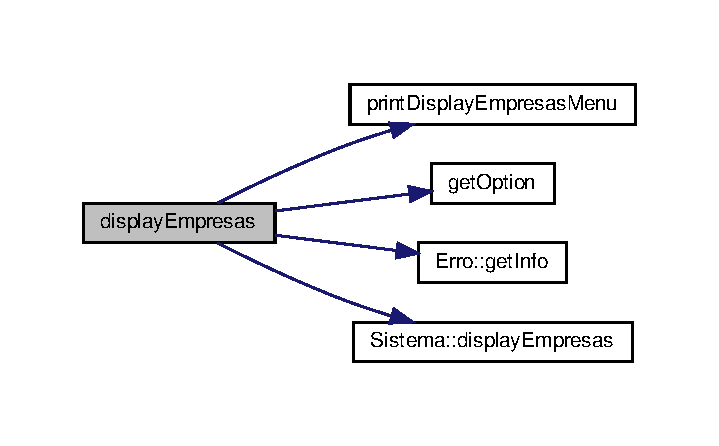
\includegraphics[width=345pt]{main_8cpp_a3a9e67719857d943301b2926cd804e8c_cgraph}
\end{center}
\end{figure}
Here is the caller graph for this function\+:
\nopagebreak
\begin{figure}[H]
\begin{center}
\leavevmode
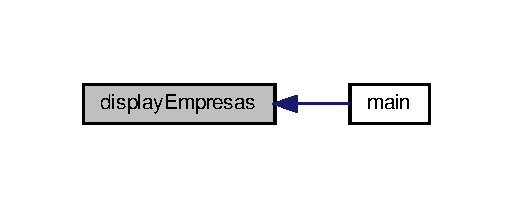
\includegraphics[width=246pt]{main_8cpp_a3a9e67719857d943301b2926cd804e8c_icgraph}
\end{center}
\end{figure}
\mbox{\Hypertarget{main_8cpp_a0932ac5f24cb3fdd2a58f8d5bbdc9507}\label{main_8cpp_a0932ac5f24cb3fdd2a58f8d5bbdc9507}} 
\index{main.\+cpp@{main.\+cpp}!display\+Rankings@{display\+Rankings}}
\index{display\+Rankings@{display\+Rankings}!main.\+cpp@{main.\+cpp}}
\subsubsection{\texorpdfstring{display\+Rankings()}{displayRankings()}}
{\footnotesize\ttfamily void display\+Rankings (\begin{DoxyParamCaption}\item[{\hyperlink{classSistema}{Sistema} $\ast$}]{sistema }\end{DoxyParamCaption})}


\begin{DoxyCode}
1031                                         \{
1032     \textcolor{keywordtype}{int} opt;
1033 
1034     \textcolor{keywordflow}{while} (\textcolor{keyword}{true}) \{
1035         \hyperlink{main_8cpp_a3da8cb0d6e5160fb3cf923a352965ff4}{printRankingMenu}();
1036 
1037         \textcolor{keywordflow}{try} \{
1038             opt = \hyperlink{main_8cpp_a69864162453f9299380c3c91be8fdca4}{getOption}(1, 7);
1039         \} \textcolor{keywordflow}{catch} (\hyperlink{classInputInvalido}{InputInvalido} &e) \{
1040             std::cout << std::endl << e.\hyperlink{classErro_abfc1e9735b259d88bb97828a23164eb0}{getInfo}() << std::endl;
1041             \textcolor{keywordflow}{continue};
1042         \}
1043 
1044         \textcolor{keywordflow}{if} (opt == 1)
1045             sistema->\hyperlink{classSistema_afc03af6008df8639b1d1878388f70886}{rankingDeGeneros}();
1046         \textcolor{keywordflow}{else} \textcolor{keywordflow}{if} (opt == 2)
1047             sistema->\hyperlink{classSistema_a922993ab8f9dd2e8eb853edf3172543b}{rankingDeIdades}();
1048         \textcolor{keywordflow}{else} \textcolor{keywordflow}{if} (opt == 3)
1049             sistema->\hyperlink{classSistema_a6e4c08a6ee3c8f5721e46f64823fd6a3}{rankingDePlataformas}();
1050         \textcolor{keywordflow}{else} \textcolor{keywordflow}{if} (opt == 4)
1051             sistema->\hyperlink{classSistema_a6fb78c2cafbf5b6703d126ef43ba43f0}{rankingDeRentabilidades}();
1052         \textcolor{keywordflow}{else} \textcolor{keywordflow}{if} (opt == 5)
1053             std::cout << \textcolor{stringliteral}{"Custo: "} << sistema->\hyperlink{classSistema_ab5d9cff098cf2551f1c31d2ba720fb3c}{custoMedioBiblioteca}() << std::endl;
1054         \textcolor{keywordflow}{else} \textcolor{keywordflow}{if} (opt==6)
1055             std::cout << \textcolor{stringliteral}{"Numero medio de titulos: "} << sistema->\hyperlink{classSistema_a588450a81753c22b0454580fde17a7a7}{nrMedioTitulos}() << 
      std::endl;
1056         \textcolor{keywordflow}{else}
1057             \textcolor{keywordflow}{break};  \textcolor{comment}{// opt = 7, o utilizador quer sair}
1058     \}
1059 
1060 \}
\end{DoxyCode}
Here is the call graph for this function\+:
\nopagebreak
\begin{figure}[H]
\begin{center}
\leavevmode
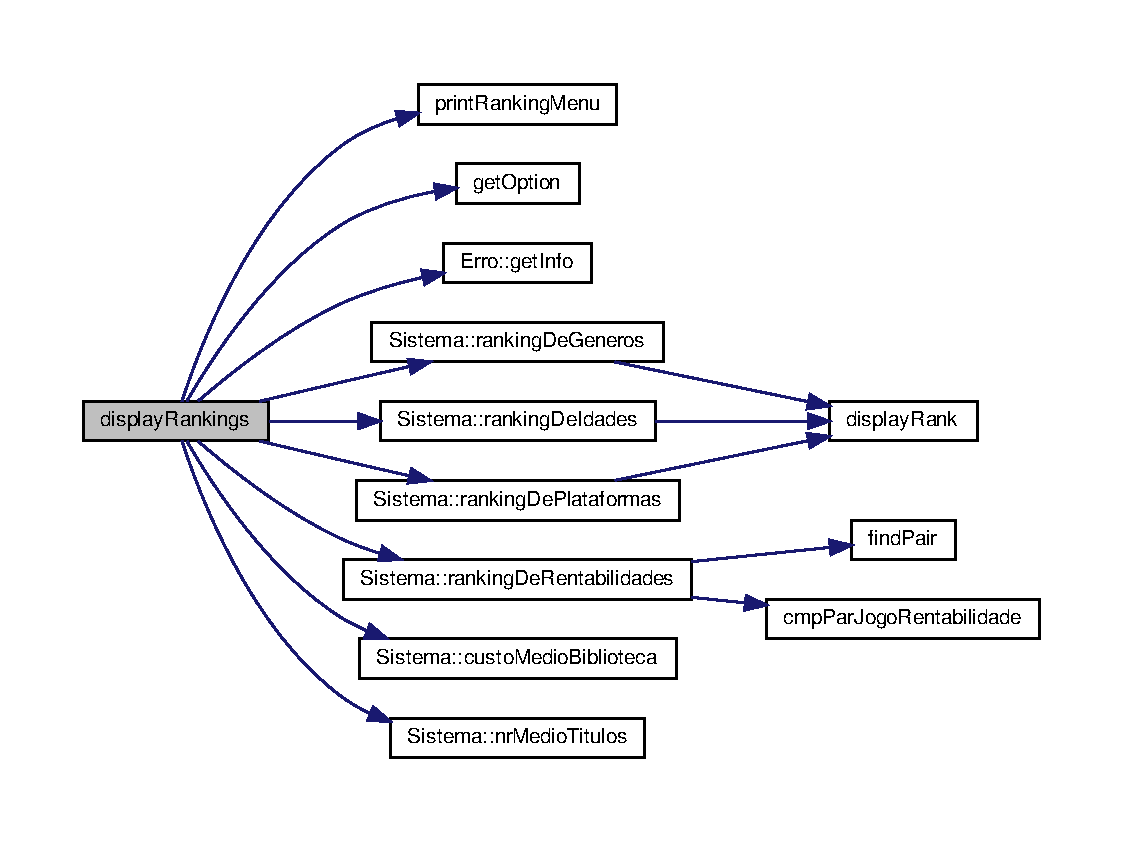
\includegraphics[width=350pt]{main_8cpp_a0932ac5f24cb3fdd2a58f8d5bbdc9507_cgraph}
\end{center}
\end{figure}
Here is the caller graph for this function\+:
\nopagebreak
\begin{figure}[H]
\begin{center}
\leavevmode
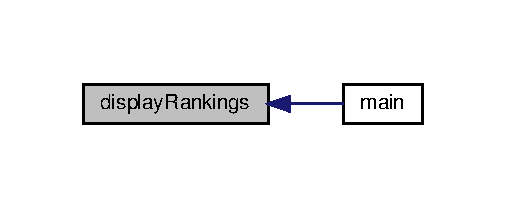
\includegraphics[width=243pt]{main_8cpp_a0932ac5f24cb3fdd2a58f8d5bbdc9507_icgraph}
\end{center}
\end{figure}
\mbox{\Hypertarget{main_8cpp_a5e58c15f905db107f320734a18f4e40d}\label{main_8cpp_a5e58c15f905db107f320734a18f4e40d}} 
\index{main.\+cpp@{main.\+cpp}!display\+Titulos@{display\+Titulos}}
\index{display\+Titulos@{display\+Titulos}!main.\+cpp@{main.\+cpp}}
\subsubsection{\texorpdfstring{display\+Titulos()}{displayTitulos()}}
{\footnotesize\ttfamily void display\+Titulos (\begin{DoxyParamCaption}\item[{\hyperlink{classSistema}{Sistema} $\ast$}]{sistema }\end{DoxyParamCaption})}


\begin{DoxyCode}
478                                        \{
479     \textcolor{keywordtype}{int} opt;
480 
481     \textcolor{comment}{// Perguntar ao utilizador o que quer fazer at� este indicar que deseja sair}
482     \textcolor{keywordflow}{while} (\textcolor{keyword}{true}) \{
483         \hyperlink{main_8cpp_a6afc9271571dfdc7288faf87e9616e7d}{printDisplayTitulosMenu}();
484 
485         \textcolor{comment}{// Pedir opcao ao utilizador e verificar se nao houve erro de input}
486         \textcolor{keywordflow}{try} \{
487             opt = \hyperlink{main_8cpp_a69864162453f9299380c3c91be8fdca4}{getOption}(1, 9);
488         \} \textcolor{keywordflow}{catch} (\hyperlink{classInputInvalido}{InputInvalido} &e) \{
489             std::cout << \textcolor{stringliteral}{"\(\backslash\)n"} << e.\hyperlink{classErro_abfc1e9735b259d88bb97828a23164eb0}{getInfo}();
490             \textcolor{keywordflow}{continue};   \textcolor{comment}{// Ir para o proximo loop , pedir nova opcao}
491         \}
492 
493         \textcolor{keywordflow}{if} (opt == 1)
494             sistema->\hyperlink{classSistema_abf82916720d1255bba6437abf0094ca6}{displayTitulos}();
495         \textcolor{keywordflow}{else} \textcolor{keywordflow}{if} (opt == 2)
496             sistema->\hyperlink{classSistema_a6dcecc2ca65f6fdedd042c7431d5ea19}{ordenaTitulos}(\textcolor{stringliteral}{"data"}, \textcolor{keyword}{true});
497         \textcolor{keywordflow}{else} \textcolor{keywordflow}{if} (opt == 3)
498             sistema->\hyperlink{classSistema_a6dcecc2ca65f6fdedd042c7431d5ea19}{ordenaTitulos}(\textcolor{stringliteral}{"data"}, \textcolor{keyword}{false});
499         \textcolor{keywordflow}{else} \textcolor{keywordflow}{if} (opt == 4)
500             sistema->\hyperlink{classSistema_a6dcecc2ca65f6fdedd042c7431d5ea19}{ordenaTitulos}(\textcolor{stringliteral}{"idade"}, \textcolor{keyword}{true});
501         \textcolor{keywordflow}{else} \textcolor{keywordflow}{if} (opt == 5)
502             sistema->\hyperlink{classSistema_a6dcecc2ca65f6fdedd042c7431d5ea19}{ordenaTitulos}(\textcolor{stringliteral}{"idade"}, \textcolor{keyword}{false});
503         \textcolor{keywordflow}{else} \textcolor{keywordflow}{if} (opt == 6)
504             sistema->\hyperlink{classSistema_a6dcecc2ca65f6fdedd042c7431d5ea19}{ordenaTitulos}(\textcolor{stringliteral}{"empresa"}, \textcolor{keyword}{true});
505         \textcolor{keywordflow}{else} \textcolor{keywordflow}{if} (opt == 7)
506             sistema->\hyperlink{classSistema_a6dcecc2ca65f6fdedd042c7431d5ea19}{ordenaTitulos}(\textcolor{stringliteral}{"empresa"}, \textcolor{keyword}{false});
507         \textcolor{keywordflow}{else} \textcolor{keywordflow}{if} (opt == 8)
508             \textcolor{keywordflow}{return};
509     \}
510 
511 \}
\end{DoxyCode}
Here is the call graph for this function\+:
\nopagebreak
\begin{figure}[H]
\begin{center}
\leavevmode
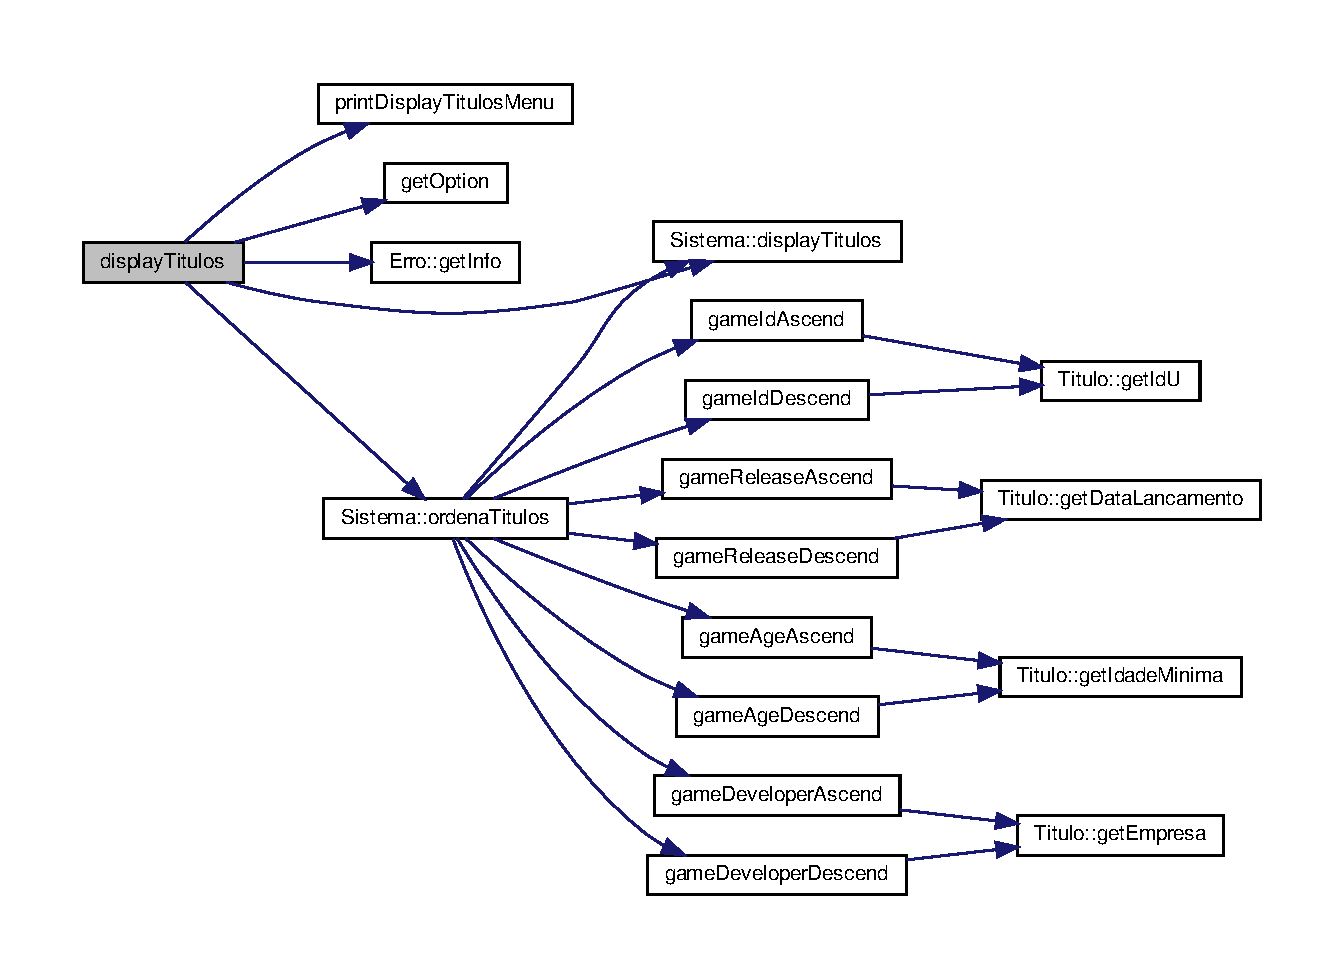
\includegraphics[width=350pt]{main_8cpp_a5e58c15f905db107f320734a18f4e40d_cgraph}
\end{center}
\end{figure}
Here is the caller graph for this function\+:
\nopagebreak
\begin{figure}[H]
\begin{center}
\leavevmode
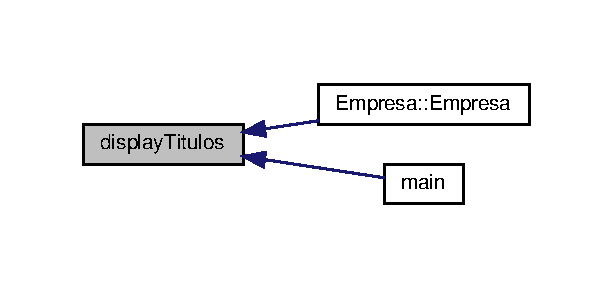
\includegraphics[width=294pt]{main_8cpp_a5e58c15f905db107f320734a18f4e40d_icgraph}
\end{center}
\end{figure}
\mbox{\Hypertarget{main_8cpp_a633c2853177204cb3a7a8033e5b9497c}\label{main_8cpp_a633c2853177204cb3a7a8033e5b9497c}} 
\index{main.\+cpp@{main.\+cpp}!display\+Utilizadores@{display\+Utilizadores}}
\index{display\+Utilizadores@{display\+Utilizadores}!main.\+cpp@{main.\+cpp}}
\subsubsection{\texorpdfstring{display\+Utilizadores()}{displayUtilizadores()}}
{\footnotesize\ttfamily void display\+Utilizadores (\begin{DoxyParamCaption}\item[{\hyperlink{classSistema}{Sistema} $\ast$}]{sistema }\end{DoxyParamCaption})}


\begin{DoxyCode}
407                                             \{
408     \textcolor{keywordtype}{int} opt;
409     \textcolor{keywordflow}{while} (\textcolor{keyword}{true}) \{
410         \hyperlink{main_8cpp_a3687e2ced7dee82b39fc1ed74674ecd5}{printDisplayUtilizadoresMenu}();
411 
412         \textcolor{keywordflow}{try} \{
413             opt = \hyperlink{main_8cpp_a69864162453f9299380c3c91be8fdca4}{getOption}(1, 8);
414         \} \textcolor{keywordflow}{catch} (\hyperlink{classInputInvalido}{InputInvalido} &e) \{
415             std::cout << \textcolor{stringliteral}{"\(\backslash\)n"} << e.\hyperlink{classErro_abfc1e9735b259d88bb97828a23164eb0}{getInfo}();
416             \textcolor{keywordflow}{continue};   \textcolor{comment}{// Ir para o proximo loop , pedir nova opcao}
417         \}
418 
419         \textcolor{keywordflow}{if} (opt == 1)
420             sistema->\hyperlink{classSistema_ac22188d7bcfb9df24776d67900b9d7fb}{displayUtilizadores}();
421         \textcolor{keywordflow}{else} \textcolor{keywordflow}{if} (opt == 2)
422             sistema->\hyperlink{classSistema_ac3b36e6798c903dd0efd102d7a5dd081}{ordenaUtilizadores}(\textcolor{stringliteral}{"idade"}, \textcolor{keyword}{true});
423         \textcolor{keywordflow}{else} \textcolor{keywordflow}{if} (opt == 3)
424             sistema->\hyperlink{classSistema_ac3b36e6798c903dd0efd102d7a5dd081}{ordenaUtilizadores}(\textcolor{stringliteral}{"idade"}, \textcolor{keyword}{false});
425         \textcolor{keywordflow}{else} \textcolor{keywordflow}{if} (opt == 4)
426             sistema->\hyperlink{classSistema_ac3b36e6798c903dd0efd102d7a5dd081}{ordenaUtilizadores}(\textcolor{stringliteral}{"jogos"}, \textcolor{keyword}{true});
427         \textcolor{keywordflow}{else} \textcolor{keywordflow}{if} (opt == 5)
428             sistema->\hyperlink{classSistema_ac3b36e6798c903dd0efd102d7a5dd081}{ordenaUtilizadores}(\textcolor{stringliteral}{"jogos"}, \textcolor{keyword}{false});
429         \textcolor{keywordflow}{else} \textcolor{keywordflow}{if} (opt == 6)
430             sistema->\hyperlink{classSistema_ac3b36e6798c903dd0efd102d7a5dd081}{ordenaUtilizadores}(\textcolor{stringliteral}{"nome"}, \textcolor{keyword}{true});
431         \textcolor{keywordflow}{else} \textcolor{keywordflow}{if} (opt == 7)
432             sistema->\hyperlink{classSistema_ac3b36e6798c903dd0efd102d7a5dd081}{ordenaUtilizadores}(\textcolor{stringliteral}{"nome"}, \textcolor{keyword}{false});
433         \textcolor{keywordflow}{else}
434             \textcolor{keywordflow}{break};
435     \}
436 \}
\end{DoxyCode}
Here is the call graph for this function\+:
\nopagebreak
\begin{figure}[H]
\begin{center}
\leavevmode
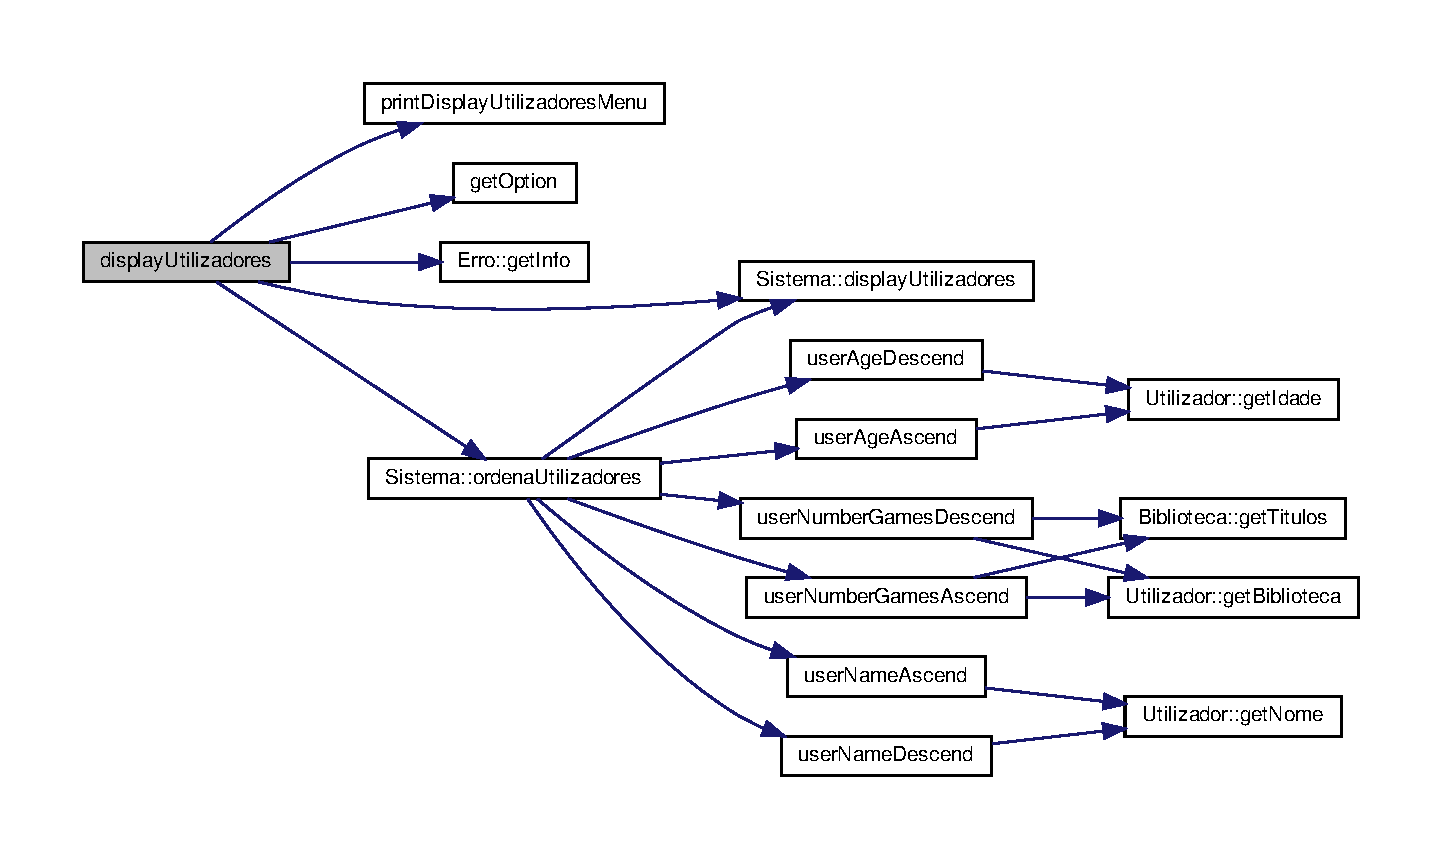
\includegraphics[width=350pt]{main_8cpp_a633c2853177204cb3a7a8033e5b9497c_cgraph}
\end{center}
\end{figure}
Here is the caller graph for this function\+:
\nopagebreak
\begin{figure}[H]
\begin{center}
\leavevmode
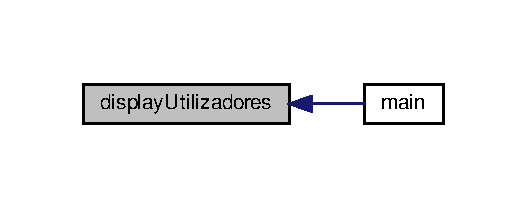
\includegraphics[width=253pt]{main_8cpp_a633c2853177204cb3a7a8033e5b9497c_icgraph}
\end{center}
\end{figure}
\mbox{\Hypertarget{main_8cpp_aa59523879399e16bcfde4f06af6ad2ff}\label{main_8cpp_aa59523879399e16bcfde4f06af6ad2ff}} 
\index{main.\+cpp@{main.\+cpp}!escolhe\+Cc@{escolhe\+Cc}}
\index{escolhe\+Cc@{escolhe\+Cc}!main.\+cpp@{main.\+cpp}}
\subsubsection{\texorpdfstring{escolhe\+Cc()}{escolheCc()}}
{\footnotesize\ttfamily void escolhe\+Cc (\begin{DoxyParamCaption}\item[{\hyperlink{classSistema}{Sistema} $\ast$}]{sistema,  }\item[{\hyperlink{classUtilizador}{Utilizador} $\ast$}]{u }\end{DoxyParamCaption})}


\begin{DoxyCode}
748                                                  \{
749     std::string id;
750     std::string saldo;
751     std::string s;
752 
753     \textcolor{keywordflow}{while} (\textcolor{keyword}{true}) \{
754         \textcolor{keywordflow}{try} \{
755             std::cout << \textcolor{stringliteral}{"Insira o id do cartao:"} << std::endl;
756             getline(std::cin, \textcolor{keywordtype}{id});
757 
758             std::cout << \textcolor{stringliteral}{"Insira o saldo a depositar:"} << std::endl;
759             getline(std::cin, saldo);
760 
761             \hyperlink{classCartaoCredito}{CartaoCredito} c(std::stof(saldo), sistema->\hyperlink{classSistema_abb768fdc8d4b8290ab4a267fc7a84a39}{getBanco}().
      \hyperlink{classBanco_a0735f07636c578666068a16f6ecccd91}{getDataAtual}(), id);
762             c.\hyperlink{classCartaoCredito_a52daaab859e37d416c00044ef0fb2f27}{atualizaDataDeValidade}();
763             u->\hyperlink{classUtilizador_a60b1025ffe94b9f2414f54cc94662cc9}{adicionaCartaoCredito}(c);
764         \} \textcolor{keywordflow}{catch} (\hyperlink{classErro}{Erro} &e) \{
765             std::cout << e.\hyperlink{classErro_abfc1e9735b259d88bb97828a23164eb0}{getInfo}() << std::endl;
766 
767             std::cout
768                     << \textcolor{stringliteral}{"Deseja desistir da insercao('s' para sair/ outro para continuar)?"}
769                     << std::endl;
770             getline(std::cin, s);
771             \textcolor{keywordflow}{if} (s == \textcolor{stringliteral}{"s"})
772                 \textcolor{keywordflow}{return};
773             \textcolor{keywordflow}{continue};
774         \}
775         \textcolor{keywordflow}{break};
776     \}
777 
778     std::cout << \textcolor{stringliteral}{"O cartao foi adicionado com sucesso."}
779             << std::endl;
780 
781 \}
\end{DoxyCode}
Here is the call graph for this function\+:
\nopagebreak
\begin{figure}[H]
\begin{center}
\leavevmode
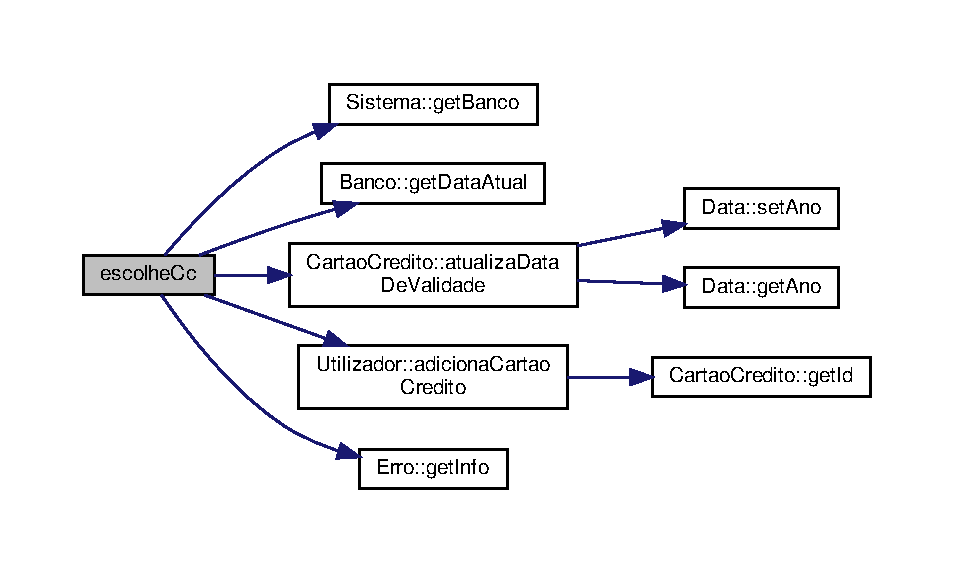
\includegraphics[width=350pt]{main_8cpp_aa59523879399e16bcfde4f06af6ad2ff_cgraph}
\end{center}
\end{figure}
Here is the caller graph for this function\+:
\nopagebreak
\begin{figure}[H]
\begin{center}
\leavevmode
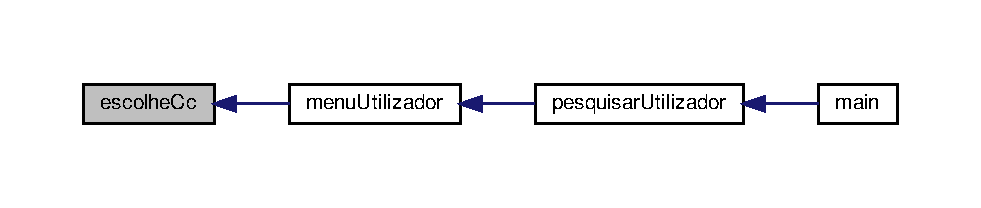
\includegraphics[width=350pt]{main_8cpp_aa59523879399e16bcfde4f06af6ad2ff_icgraph}
\end{center}
\end{figure}
\mbox{\Hypertarget{main_8cpp_af8f302c02e726f24c5f7ddea9cd7f17d}\label{main_8cpp_af8f302c02e726f24c5f7ddea9cd7f17d}} 
\index{main.\+cpp@{main.\+cpp}!escolhe\+Titulo@{escolhe\+Titulo}}
\index{escolhe\+Titulo@{escolhe\+Titulo}!main.\+cpp@{main.\+cpp}}
\subsubsection{\texorpdfstring{escolhe\+Titulo()}{escolheTitulo()}}
{\footnotesize\ttfamily void escolhe\+Titulo (\begin{DoxyParamCaption}\item[{\hyperlink{classSistema}{Sistema} $\ast$}]{sistema,  }\item[{\hyperlink{classUtilizador}{Utilizador} $\ast$}]{u }\end{DoxyParamCaption})}


\begin{DoxyCode}
569                                                      \{
570     std::string titulo;
571     std::string plataforma;
572     std::string s;
573 
574     \textcolor{keywordflow}{while} (\textcolor{keyword}{true}) \{
575         std::cout << \textcolor{stringliteral}{"Insira o nome do titulo"} << std::endl;
576         getline(std::cin, titulo);
577         std::cout << \textcolor{stringliteral}{"Insira a plataforma"} << std::endl;
578         getline(std::cin, plataforma);
579 
580         \textcolor{keywordflow}{try} \{
581             \hyperlink{classTitulo}{Titulo} * t = sistema->\hyperlink{classSistema_a0fb81a4685bb24024295c89d22d6d719}{pesquisaJogo}(titulo, plataforma);
582 
583             \textcolor{keywordflow}{if} (u->\hyperlink{classUtilizador_ad0ebe5ff80aa77145ec4b0ce5473102c}{getCc}().size() == 0) \{
584                 std::cout << \textcolor{stringliteral}{"O utilizador nao tem cartoes!"} << std::endl;
585             \}
586             \textcolor{keywordflow}{for} (\textcolor{keyword}{auto} & cartao : u->\hyperlink{classUtilizador_ad0ebe5ff80aa77145ec4b0ce5473102c}{getCc}()) \{
587                 \textcolor{keywordflow}{try} \{
588                     u->\hyperlink{classUtilizador_ac08a744b9d9d2aca0bd22c60e0beaa83}{AdicionaTitulo}(t, cartao);
589                     u->\hyperlink{classUtilizador_aa47c2fe835a73a23664149ccc7fbc10f}{removeWishList}(t);
590                     sistema->\hyperlink{classSistema_a0d6da6cf391b19d37001dab66c861b93}{dataValida}(cartao);
591                     sistema->\hyperlink{classSistema_a59ff239e4793308c979cccf796a72f23}{removeAsleepUsers}(plataforma,u);
592                 \}
593                 \textcolor{keywordflow}{catch} (\hyperlink{classTituloJaAdicionado}{TituloJaAdicionado} &e) \{
594                     \textcolor{keywordflow}{throw}(e);
595                 \}
596                 \textcolor{keywordflow}{catch} (\hyperlink{classErro}{Erro} &e) \{
597                     std::cout << e.\hyperlink{classErro_abfc1e9735b259d88bb97828a23164eb0}{getInfo}() << std::endl;
598                     \textcolor{keywordflow}{continue};
599                 \}
600                 std::cout << \textcolor{stringliteral}{"Adicionou o titulo "} << titulo
601                         << \textcolor{stringliteral}{" a biblioteca do utilizador, removendo "} << t->
      \hyperlink{classTitulo_a93725bdc2e98350e47b54fd76c0fa236}{getPreco}()
602                         << \textcolor{stringliteral}{" euros ao cartao "} << cartao.getId() << std::endl;
603                 \textcolor{keywordflow}{break};
604             \}
605 
606         \} \textcolor{keywordflow}{catch} (\hyperlink{classErro}{Erro} &e) \{
607             std::cout << e.\hyperlink{classErro_abfc1e9735b259d88bb97828a23164eb0}{getInfo}() << std::endl;
608             std::cout
609                     << \textcolor{stringliteral}{"Deseja desistir da procura('s' para sair/ outro para continuar)?"}
610                     << std::endl;
611             getline(std::cin, s);
612             \textcolor{keywordflow}{if} (s == \textcolor{stringliteral}{"s"})
613                 \textcolor{keywordflow}{return};
614 
615             \textcolor{keywordflow}{continue};
616         \}
617         \textcolor{keywordflow}{break};
618     \}
619 \}
\end{DoxyCode}
Here is the call graph for this function\+:
\nopagebreak
\begin{figure}[H]
\begin{center}
\leavevmode
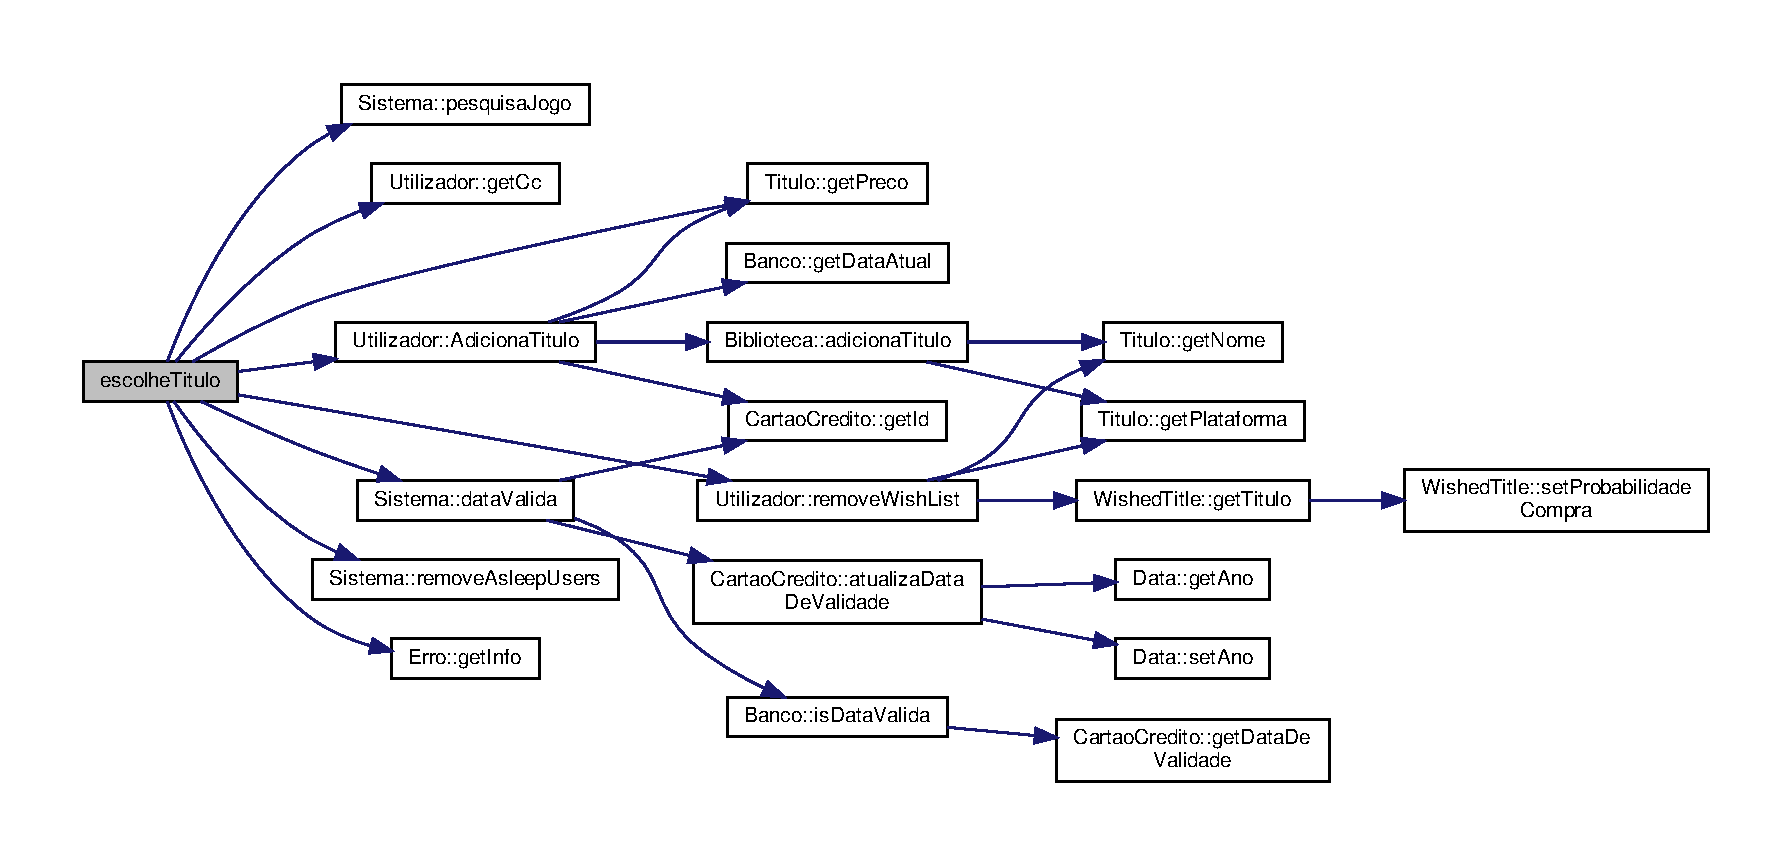
\includegraphics[width=350pt]{main_8cpp_af8f302c02e726f24c5f7ddea9cd7f17d_cgraph}
\end{center}
\end{figure}
Here is the caller graph for this function\+:
\nopagebreak
\begin{figure}[H]
\begin{center}
\leavevmode
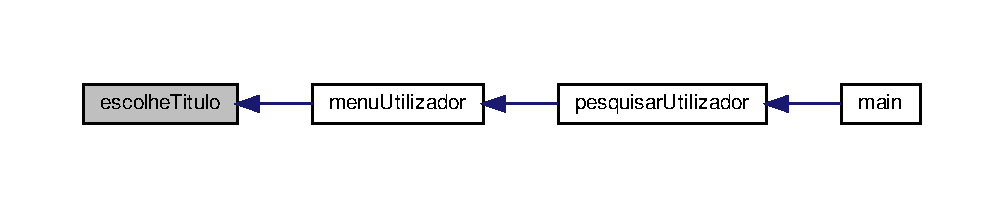
\includegraphics[width=350pt]{main_8cpp_af8f302c02e726f24c5f7ddea9cd7f17d_icgraph}
\end{center}
\end{figure}
\mbox{\Hypertarget{main_8cpp_a69864162453f9299380c3c91be8fdca4}\label{main_8cpp_a69864162453f9299380c3c91be8fdca4}} 
\index{main.\+cpp@{main.\+cpp}!get\+Option@{get\+Option}}
\index{get\+Option@{get\+Option}!main.\+cpp@{main.\+cpp}}
\subsubsection{\texorpdfstring{get\+Option()}{getOption()}}
{\footnotesize\ttfamily int get\+Option (\begin{DoxyParamCaption}\item[{int}]{min,  }\item[{int}]{max }\end{DoxyParamCaption})}


\begin{DoxyCode}
10                                 \{
11     \textcolor{keywordtype}{int} opt;
12 
13     \textcolor{comment}{// Get the option}
14     std::cout << \textcolor{stringliteral}{">>> "};
15     std::cin >> opt;
16 
17     \textcolor{comment}{// Check if not a number was entered}
18     \textcolor{keywordflow}{if} (std::cin.fail()) \{
19         \textcolor{comment}{// Clear the cin error flags and the stream content, throw the error}
20         std::cin.clear();
21         std::cin.ignore(1000, \textcolor{charliteral}{'\(\backslash\)n'});
22         \textcolor{keywordflow}{throw}(\hyperlink{classInputInvalido}{InputInvalido}(\textcolor{stringliteral}{"Input Invalido!"}));
23     \}
24 
25     \textcolor{comment}{// Clear the cin stream even if no error occured, to ensure the stream always stays clean}
26     std::cin.ignore(1000, \textcolor{charliteral}{'\(\backslash\)n'});
27 
28     \textcolor{comment}{// Check if the option is valid}
29     \textcolor{keywordflow}{if} (opt >= min && opt <= max)
30         \textcolor{keywordflow}{return} opt;
31     \textcolor{keywordflow}{else}
32         \textcolor{keywordflow}{throw}(\hyperlink{classInputInvalido}{InputInvalido}(\textcolor{stringliteral}{"Opcao Invalida!"}));
33 \}
\end{DoxyCode}
Here is the caller graph for this function\+:
\nopagebreak
\begin{figure}[H]
\begin{center}
\leavevmode
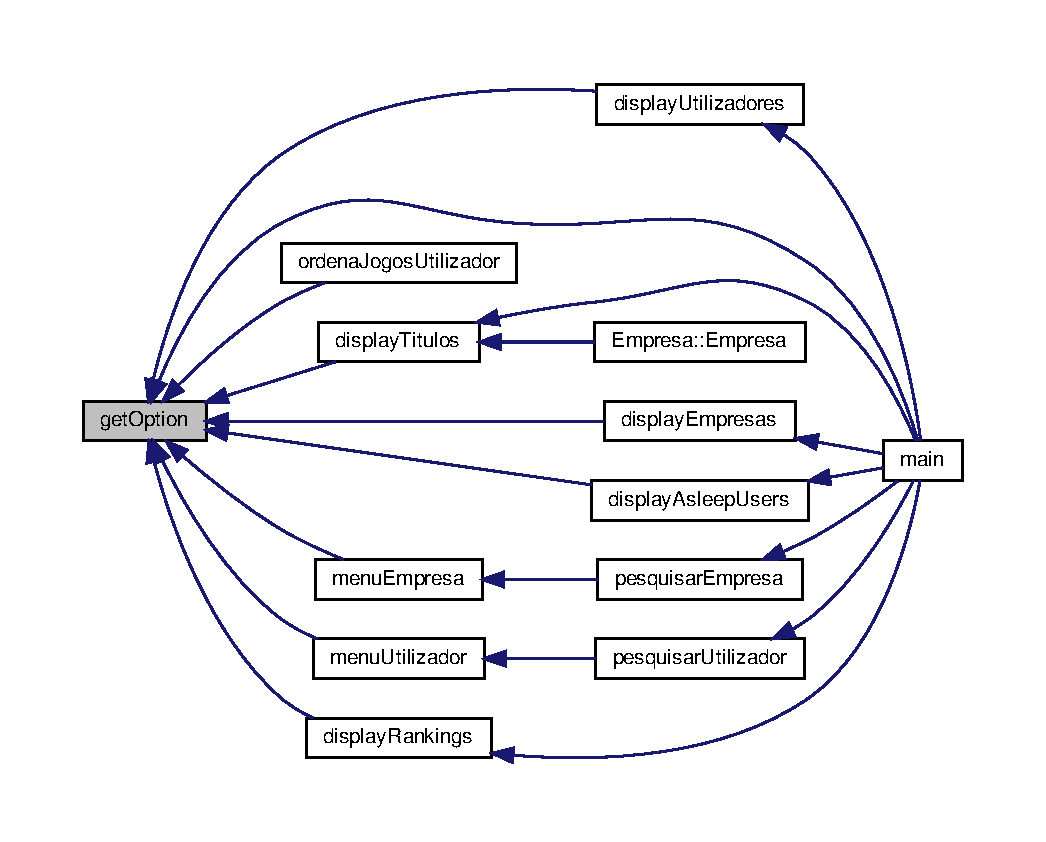
\includegraphics[width=350pt]{main_8cpp_a69864162453f9299380c3c91be8fdca4_icgraph}
\end{center}
\end{figure}
\mbox{\Hypertarget{main_8cpp_a6c175a1424e435dba38c472eaf2f5535}\label{main_8cpp_a6c175a1424e435dba38c472eaf2f5535}} 
\index{main.\+cpp@{main.\+cpp}!is\+\_\+digits@{is\+\_\+digits}}
\index{is\+\_\+digits@{is\+\_\+digits}!main.\+cpp@{main.\+cpp}}
\subsubsection{\texorpdfstring{is\+\_\+digits()}{is\_digits()}}
{\footnotesize\ttfamily bool is\+\_\+digits (\begin{DoxyParamCaption}\item[{const std\+::string \&}]{str }\end{DoxyParamCaption})}


\begin{DoxyCode}
352 \{
353     \textcolor{keywordflow}{return} std::all\_of(str.begin(), str.end(), ::isdigit);
354 \}
\end{DoxyCode}
Here is the caller graph for this function\+:
\nopagebreak
\begin{figure}[H]
\begin{center}
\leavevmode
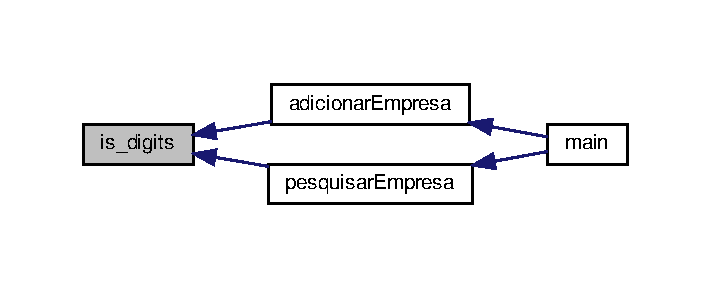
\includegraphics[width=341pt]{main_8cpp_a6c175a1424e435dba38c472eaf2f5535_icgraph}
\end{center}
\end{figure}
\mbox{\Hypertarget{main_8cpp_afdd4f73eaf1ae01f9f045850fe275884}\label{main_8cpp_afdd4f73eaf1ae01f9f045850fe275884}} 
\index{main.\+cpp@{main.\+cpp}!ler\+Data@{ler\+Data}}
\index{ler\+Data@{ler\+Data}!main.\+cpp@{main.\+cpp}}
\subsubsection{\texorpdfstring{ler\+Data()}{lerData()}}
{\footnotesize\ttfamily void ler\+Data (\begin{DoxyParamCaption}\item[{std\+::string}]{data }\end{DoxyParamCaption})}


\begin{DoxyCode}
168                              \{
169 
170     \textcolor{comment}{// Verificar se esta no formato v�lido (DD/MM/AAAA)}
171     \textcolor{keywordflow}{if} (data.size() != 10)          \textcolor{comment}{// Verificar se a data tem o tamanho correto}
172         \textcolor{keywordflow}{throw}(\hyperlink{classDataInvalida}{DataInvalida}(\textcolor{stringliteral}{"Data Invalida!"}));
173     \textcolor{keywordflow}{else} \textcolor{keywordflow}{if} ((data.at(2) != \textcolor{charliteral}{'/'}) || (data.at(5) != \textcolor{charliteral}{'/'}))\textcolor{comment}{// Verificar se dia, mes e ano estao separados por
       um traco}
174         \textcolor{keywordflow}{throw}(\hyperlink{classDataInvalida}{DataInvalida}(\textcolor{stringliteral}{"Data Invalida!"}));
175     \textcolor{keywordflow}{else} \textcolor{keywordflow}{if} ((data.at(0) < \textcolor{charliteral}{'0'}) || (data.at(0) > \textcolor{charliteral}{'9'}))\textcolor{comment}{// Verificar se Dx � um digito}
176         \textcolor{keywordflow}{throw}(\hyperlink{classDataInvalida}{DataInvalida}(\textcolor{stringliteral}{"Data Invalida!"}));
177     \textcolor{keywordflow}{else} \textcolor{keywordflow}{if} ((data.at(1) < \textcolor{charliteral}{'0'}) || (data.at(1) > \textcolor{charliteral}{'9'}))\textcolor{comment}{// Verificar se xD � um digito}
178         \textcolor{keywordflow}{throw}(\hyperlink{classDataInvalida}{DataInvalida}(\textcolor{stringliteral}{"Data Invalida!"}));
179     \textcolor{keywordflow}{else} \textcolor{keywordflow}{if} ((data.at(3) < \textcolor{charliteral}{'0'}) || (data.at(3) > \textcolor{charliteral}{'9'}))\textcolor{comment}{// Verificar se Mx � um digito}
180         \textcolor{keywordflow}{throw}(\hyperlink{classDataInvalida}{DataInvalida}(\textcolor{stringliteral}{"Data Invalida!"}));
181     \textcolor{keywordflow}{else} \textcolor{keywordflow}{if} ((data.at(4) < \textcolor{charliteral}{'0'}) || (data.at(4) > \textcolor{charliteral}{'9'}))\textcolor{comment}{// Verificar se xM � um digito}
182         \textcolor{keywordflow}{throw}(\hyperlink{classDataInvalida}{DataInvalida}(\textcolor{stringliteral}{"Data Invalida!"}));
183     \textcolor{keywordflow}{else} \textcolor{keywordflow}{if} ((data.at(6) < \textcolor{charliteral}{'0'}) || (data.at(6) > \textcolor{charliteral}{'9'}))\textcolor{comment}{// Verificar se Axxx � um d�gito}
184         \textcolor{keywordflow}{throw}(\hyperlink{classDataInvalida}{DataInvalida}(\textcolor{stringliteral}{"Data Invalida!"}));
185     \textcolor{keywordflow}{else} \textcolor{keywordflow}{if} ((data.at(7) < \textcolor{charliteral}{'0'}) || (data.at(7) > \textcolor{charliteral}{'9'}))\textcolor{comment}{// Verificar se xAxx � um d�gito}
186         \textcolor{keywordflow}{throw}(\hyperlink{classDataInvalida}{DataInvalida}(\textcolor{stringliteral}{"Data Invalida!"}));
187     \textcolor{keywordflow}{else} \textcolor{keywordflow}{if} ((data.at(8) < \textcolor{charliteral}{'0'}) || (data.at(8) > \textcolor{charliteral}{'9'}))\textcolor{comment}{// Verificar se xxAx � um d�gito}
188         \textcolor{keywordflow}{throw}(\hyperlink{classDataInvalida}{DataInvalida}(\textcolor{stringliteral}{"Data Invalida!"}));
189     \textcolor{keywordflow}{else} \textcolor{keywordflow}{if} ((data.at(9) < \textcolor{charliteral}{'0'}) || (data.at(9) > \textcolor{charliteral}{'9'}))\textcolor{comment}{// Verificar se xxxA � um d�gito}
190         \textcolor{keywordflow}{throw}(\hyperlink{classDataInvalida}{DataInvalida}(\textcolor{stringliteral}{"Data Invalida!"}));
191 
192     \textcolor{comment}{// Verificar se a data segue os padr�es normais de datas}
193     \textcolor{keywordtype}{int} dia = stoi(data.substr(0, 2));
194     \textcolor{keywordtype}{int} mes = stoi(data.substr(3, 2));
195     \textcolor{keywordtype}{int} ano = stoi(data.substr(6, 4));
196 
197     \textcolor{comment}{// Verificar se o mes esta dentro dos limites reais}
198     \textcolor{keywordflow}{if} (mes < 0 || mes > 12)
199         \textcolor{keywordflow}{throw}(\hyperlink{classDataInvalida}{DataInvalida}(\textcolor{stringliteral}{"Data Invalida!"}));
200 
201     \textcolor{keywordflow}{switch} (mes) \{
202     \textcolor{keywordflow}{case} 1:
203     \textcolor{keywordflow}{case} 3:
204     \textcolor{keywordflow}{case} 5:
205     \textcolor{keywordflow}{case} 7:
206     \textcolor{keywordflow}{case} 8:
207     \textcolor{keywordflow}{case} 10:
208     \textcolor{keywordflow}{case} 12:        \textcolor{comment}{// Meses com 31 dias}
209         \textcolor{keywordflow}{if} ((dia < 0) || (dia > 31))
210             \textcolor{keywordflow}{throw}(\hyperlink{classDataInvalida}{DataInvalida}(\textcolor{stringliteral}{"Data Incorreta!"}));
211         \textcolor{keywordflow}{break};
212     \textcolor{keywordflow}{case} 4:
213     \textcolor{keywordflow}{case} 6:
214     \textcolor{keywordflow}{case} 9:
215     \textcolor{keywordflow}{case} 11:                                \textcolor{comment}{// Meses com 30 dias}
216         \textcolor{keywordflow}{if} ((dia < 0) || (dia > 30))
217             \textcolor{keywordflow}{throw}(\hyperlink{classDataInvalida}{DataInvalida}(\textcolor{stringliteral}{"Data Incorreta!"}));
218         \textcolor{keywordflow}{break};
219     \textcolor{keywordflow}{case} 2:                                                         \textcolor{comment}{// Fevereiro}
220         \textcolor{keywordflow}{if} ((dia < 0) || (dia > 29))
221             \textcolor{keywordflow}{throw}(\hyperlink{classDataInvalida}{DataInvalida}(\textcolor{stringliteral}{"Data Incorreta!"}));
222         \textcolor{keywordflow}{else} \textcolor{keywordflow}{if} ((dia == 29) && (ano % 4 != 0))
223             \textcolor{keywordflow}{throw}(\hyperlink{classDataInvalida}{DataInvalida}(\textcolor{stringliteral}{"Data Incorreta!"}));
224         \textcolor{keywordflow}{break};
225     \}
226 
227 
228     \textcolor{keywordflow}{return};
229 \}
\end{DoxyCode}
Here is the caller graph for this function\+:
\nopagebreak
\begin{figure}[H]
\begin{center}
\leavevmode
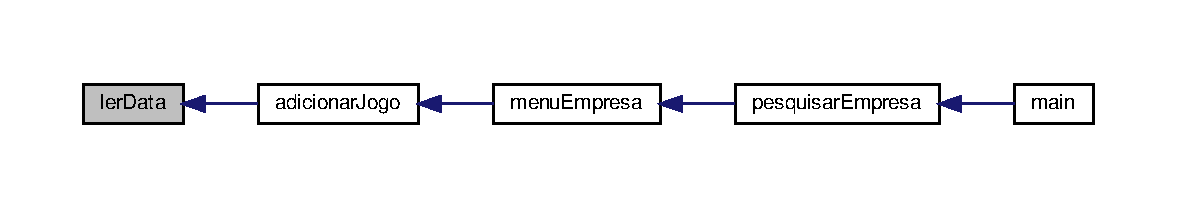
\includegraphics[width=350pt]{main_8cpp_afdd4f73eaf1ae01f9f045850fe275884_icgraph}
\end{center}
\end{figure}
\mbox{\Hypertarget{main_8cpp_ae66f6b31b5ad750f1fe042a706a4e3d4}\label{main_8cpp_ae66f6b31b5ad750f1fe042a706a4e3d4}} 
\index{main.\+cpp@{main.\+cpp}!main@{main}}
\index{main@{main}!main.\+cpp@{main.\+cpp}}
\subsubsection{\texorpdfstring{main()}{main()}}
{\footnotesize\ttfamily int main (\begin{DoxyParamCaption}{ }\end{DoxyParamCaption})}


\begin{DoxyCode}
1061            \{
1062     \hyperlink{main_8cpp_a89a9bf7f76b270a3a9fc783b4009586c}{printWelcomeMenu}();
1063     \hyperlink{classSistema}{Sistema} * sistema = \textcolor{keyword}{new} \hyperlink{classSistema}{Sistema};
1064 
1065     sistema->\hyperlink{classSistema_aeffb6968ea519c472e90dfec1a2a072e}{readEmpresas}();
1066     sistema->\hyperlink{classSistema_a187636be859f6a6dd7427cb781cd11a5}{readUtilizadores}();
1067 
1068     \textcolor{keywordflow}{for}(\textcolor{keyword}{auto} it: sistema->\hyperlink{classSistema_acb9f4d8c3ee7d1a24f8784c379f660df}{getJogadores}())\{
1069         it->printPublicidade();
1070     \}
1071 
1072     \textcolor{keywordtype}{int} opt;
1073 
1074     \textcolor{comment}{// Perguntar ao utilizador o que quer fazer ate este indicar que deseja sair}
1075     \textcolor{keywordflow}{while} (\textcolor{keyword}{true}) \{
1076         \hyperlink{main_8cpp_af9dce1973196a5934ee5ec20ea417324}{printMainMenu}();
1077 
1078         sistema->\hyperlink{classSistema_a265736b1b095448d7343b199a1ade7e5}{atualizaAsleepUsers}();
1079 
1080         \textcolor{comment}{// Pedir opcao ao utilizador e verificar se nao houve erro de input}
1081         \textcolor{keywordflow}{try} \{
1082             opt = \hyperlink{main_8cpp_a69864162453f9299380c3c91be8fdca4}{getOption}(1, 11);
1083         \} \textcolor{keywordflow}{catch} (\hyperlink{classInputInvalido}{InputInvalido} &e) \{
1084             std::cout << \textcolor{stringliteral}{"\(\backslash\)n"} << e.\hyperlink{classErro_abfc1e9735b259d88bb97828a23164eb0}{getInfo}();
1085             \textcolor{keywordflow}{continue};   \textcolor{comment}{// Ir para o proximo loop , pedir nova opcao}
1086         \}
1087 
1088         \textcolor{keywordflow}{if} (opt == 1)
1089             \hyperlink{main_8cpp_a5e58c15f905db107f320734a18f4e40d}{displayTitulos}(sistema);
1090         \textcolor{keywordflow}{else} \textcolor{keywordflow}{if} (opt == 2)
1091             \hyperlink{main_8cpp_a874c5a99e7c57fa9c6bc09580292dab9}{adicionarUtilizador}(sistema);
1092         \textcolor{keywordflow}{else} \textcolor{keywordflow}{if} (opt == 3)
1093             \hyperlink{main_8cpp_a633c2853177204cb3a7a8033e5b9497c}{displayUtilizadores}(sistema);
1094         \textcolor{keywordflow}{else} \textcolor{keywordflow}{if} (opt == 4)
1095             \hyperlink{main_8cpp_ab36c65bcfd56b6a29bee851e57462ad2}{pesquisarUtilizador}(sistema);
1096         \textcolor{keywordflow}{else} \textcolor{keywordflow}{if} (opt == 5)
1097             \hyperlink{main_8cpp_a84916567707f41d606bb5cbdd44d6c17}{pesquisarJogo}(sistema);
1098         \textcolor{keywordflow}{else} \textcolor{keywordflow}{if} (opt == 6)
1099             \hyperlink{main_8cpp_a0932ac5f24cb3fdd2a58f8d5bbdc9507}{displayRankings}(sistema);
1100         \textcolor{keywordflow}{else} \textcolor{keywordflow}{if} (opt == 7)
1101             \hyperlink{main_8cpp_ae1e120878470259b19387b335d21eb69}{adicionarEmpresa}(sistema);
1102         \textcolor{keywordflow}{else} \textcolor{keywordflow}{if} (opt == 8)
1103             \hyperlink{main_8cpp_ab5d3bc5e7f94dade3058f2afb385c8a4}{pesquisarEmpresa}(sistema);
1104         \textcolor{keywordflow}{else} \textcolor{keywordflow}{if} (opt == 9)
1105             \hyperlink{main_8cpp_a3a9e67719857d943301b2926cd804e8c}{displayEmpresas}(sistema);
1106         \textcolor{keywordflow}{else} \textcolor{keywordflow}{if} (opt == 10)
1107             \hyperlink{main_8cpp_ae8e4ad4c7859f965d182b4bfb5e16abc}{displayAsleepUsers}(sistema);
1108         \textcolor{keywordflow}{else} \{
1109             std::cout << \textcolor{stringliteral}{"Adeus!"} << std::endl;
1110             \textcolor{keywordflow}{break};
1111         \}
1112     \}
1113 
1114 
1115     sistema->\hyperlink{classSistema_af25036f1b2d4abc30447c45f3c3237b8}{saveUtilizadores}();
1116     sistema->\hyperlink{classSistema_ada4619fbedcb5a07d807545caebd5c57}{saveEmpresas}();
1117     \textcolor{keyword}{delete}(sistema);
1118 
1119 
1120 
1121     \textcolor{keywordflow}{return} 0;
1122 \}
\end{DoxyCode}
Here is the call graph for this function\+:
\nopagebreak
\begin{figure}[H]
\begin{center}
\leavevmode
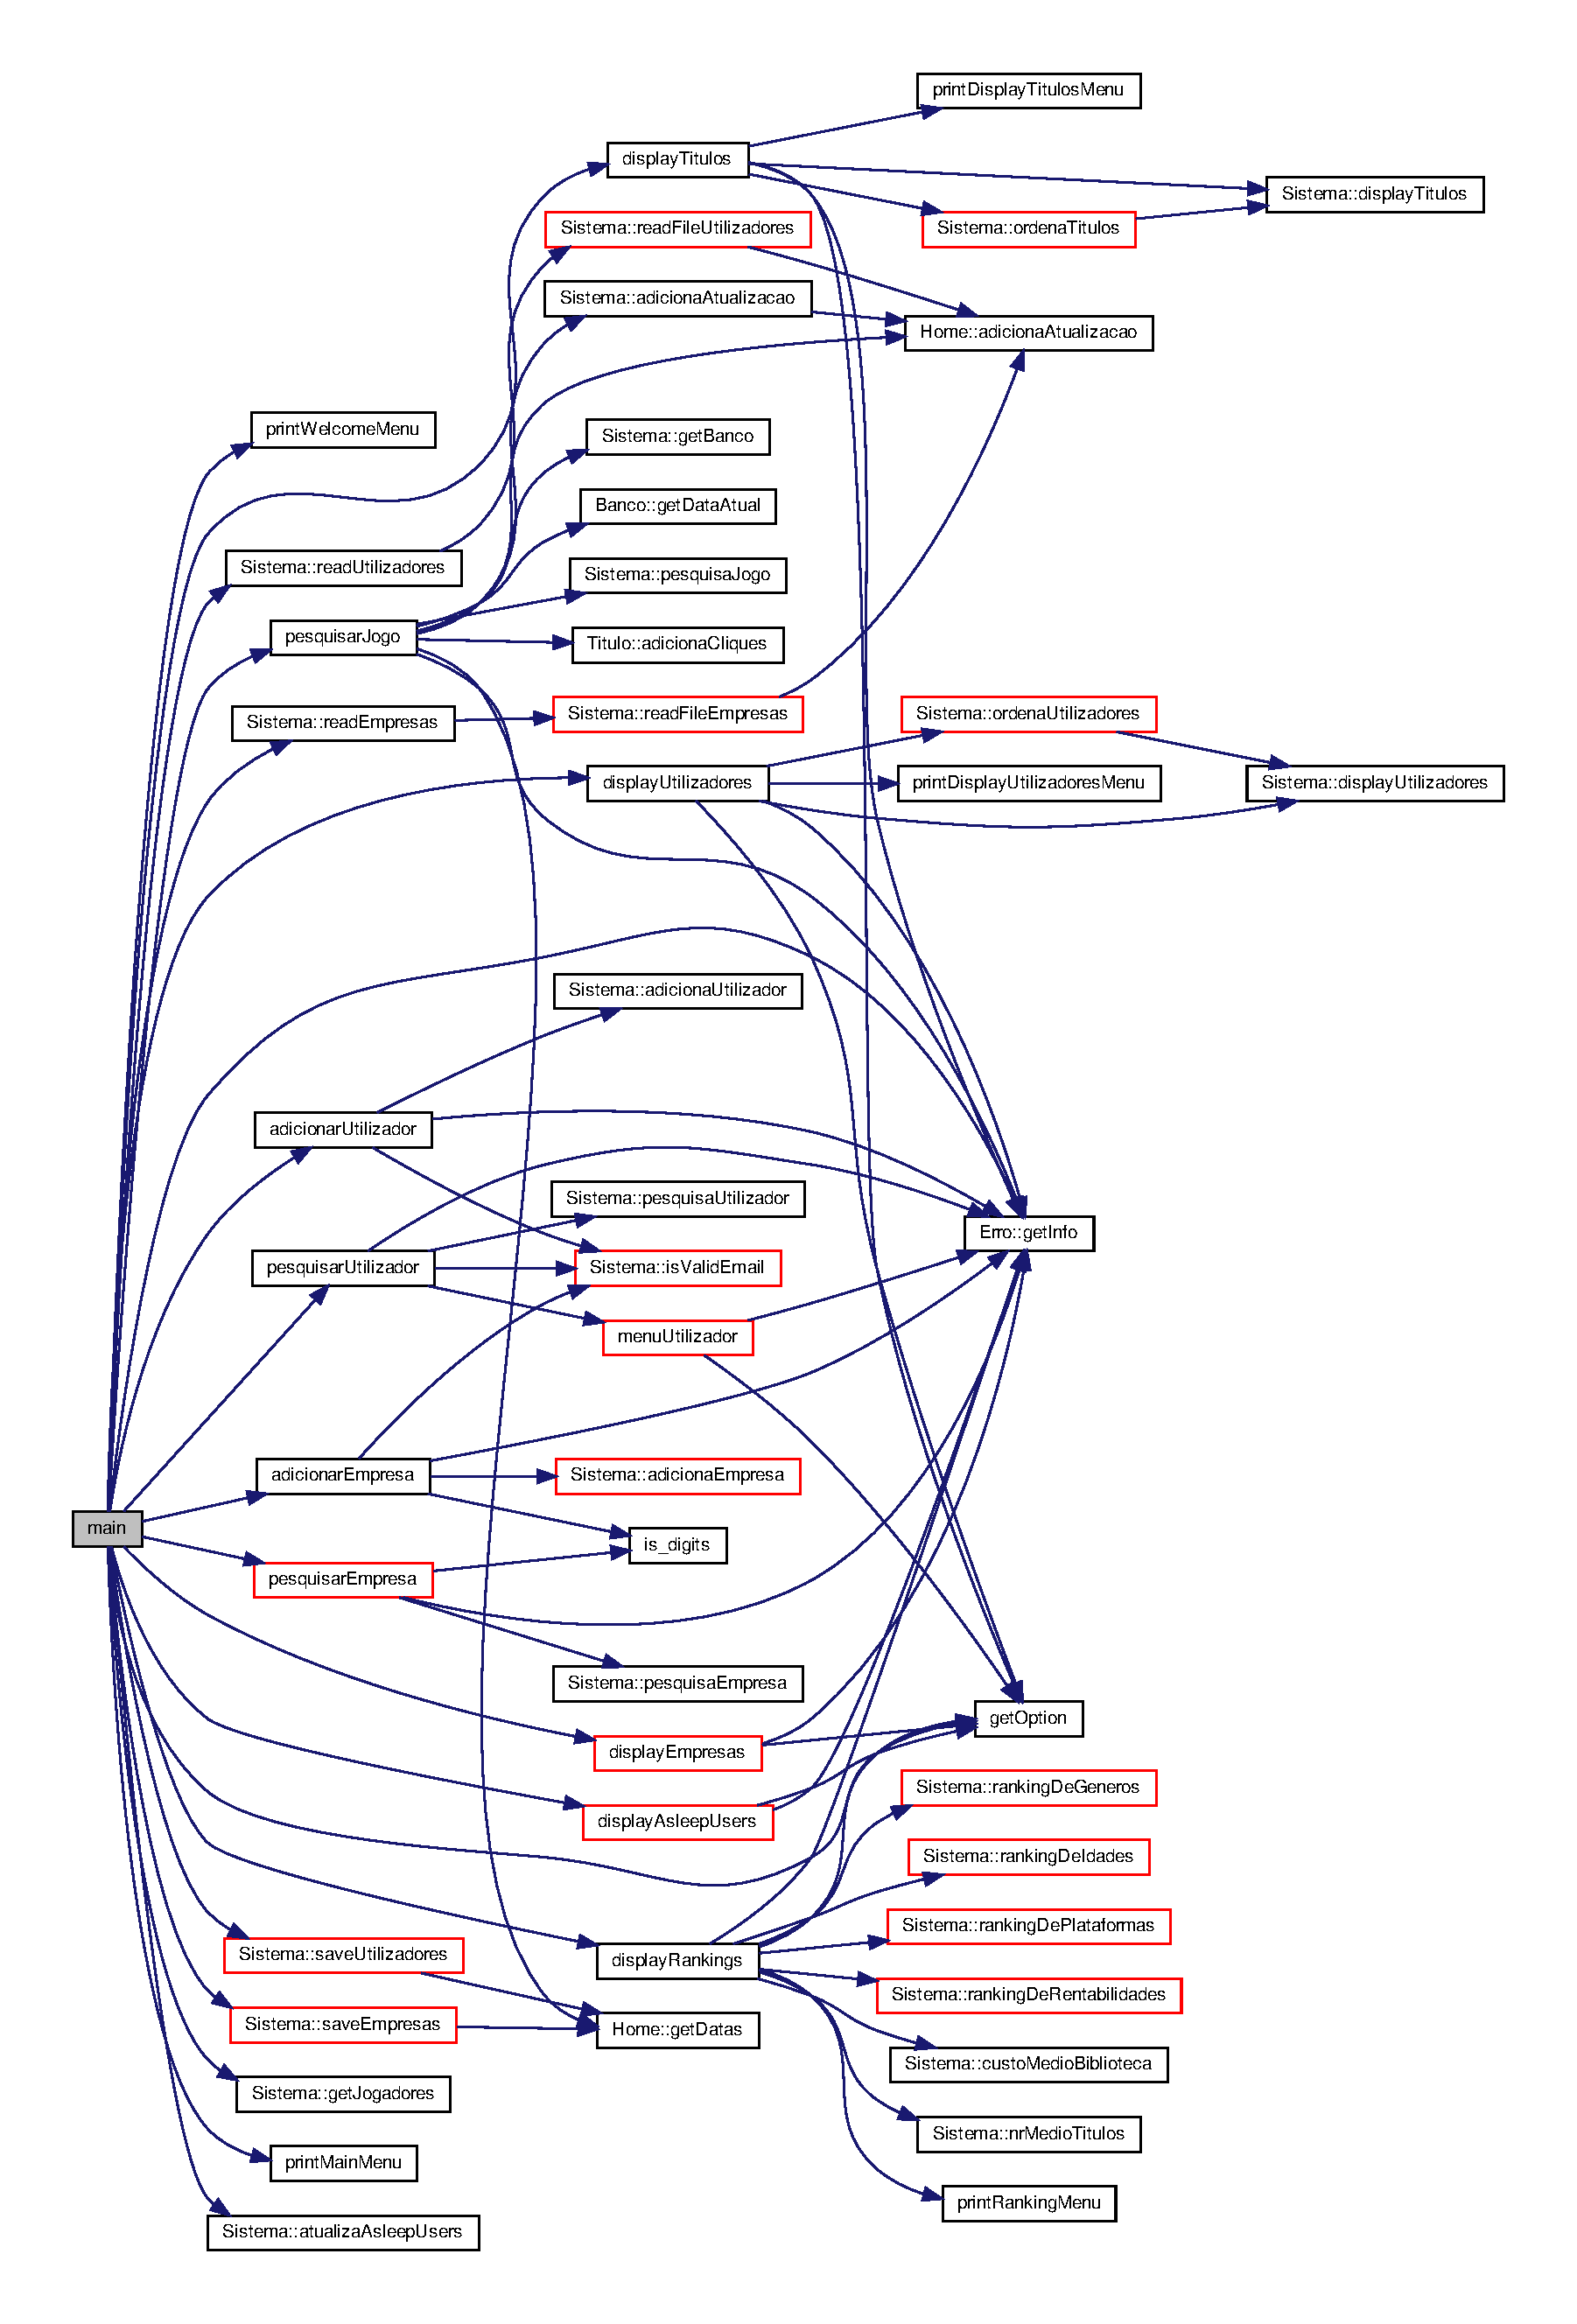
\includegraphics[width=350pt]{main_8cpp_ae66f6b31b5ad750f1fe042a706a4e3d4_cgraph}
\end{center}
\end{figure}
\mbox{\Hypertarget{main_8cpp_a175192136cbe59d60bb80a1cd975fb68}\label{main_8cpp_a175192136cbe59d60bb80a1cd975fb68}} 
\index{main.\+cpp@{main.\+cpp}!menu\+Empresa@{menu\+Empresa}}
\index{menu\+Empresa@{menu\+Empresa}!main.\+cpp@{main.\+cpp}}
\subsubsection{\texorpdfstring{menu\+Empresa()}{menuEmpresa()}}
{\footnotesize\ttfamily void menu\+Empresa (\begin{DoxyParamCaption}\item[{\hyperlink{classSistema}{Sistema} $\ast$}]{sistema,  }\item[{\hyperlink{classEmpresa}{Empresa} $\ast$}]{empresa }\end{DoxyParamCaption})}


\begin{DoxyCode}
846                                                        \{
847     \textcolor{keywordtype}{int} opt;
848 
849         \textcolor{keywordflow}{while} (\textcolor{keyword}{true}) \{
850             \hyperlink{main_8cpp_a28b549948b369d4db7a926ec0cfd6e77}{printEmpresaMenu}();
851 
852             \textcolor{keywordflow}{try} \{
853                 opt = \hyperlink{main_8cpp_a69864162453f9299380c3c91be8fdca4}{getOption}(1, 4);
854             \} \textcolor{keywordflow}{catch} (\hyperlink{classInputInvalido}{InputInvalido} &e) \{
855                 std::cout << \textcolor{stringliteral}{"\(\backslash\)n"} << e.\hyperlink{classErro_abfc1e9735b259d88bb97828a23164eb0}{getInfo}();
856                 \textcolor{keywordflow}{continue};
857             \}
858 
859             \textcolor{keywordflow}{if} (opt == 1)
860                 \hyperlink{main_8cpp_af223924a460aa7610e351d33b9105191}{adicionarJogo}(sistema,empresa->\hyperlink{classEmpresa_a99bc2de98a0c0348abb74c93e6e7159e}{getNomeEmpresa}());
861             \textcolor{keywordflow}{else} \textcolor{keywordflow}{if} (opt == 2) \{
862                 std::cout << \textcolor{stringliteral}{"Numero de telemovel: "} << empresa->\hyperlink{classEmpresa_a19396f860d9b17f94bd262ba093d76eb}{getContactos}().
      \hyperlink{structcontactos_a09e1d4029e1eb91fc9ec76e4b4b6d48a}{numeroTelemovel}<<std::endl;
863                 std::cout << \textcolor{stringliteral}{"Email: "} << empresa->\hyperlink{classEmpresa_a19396f860d9b17f94bd262ba093d76eb}{getContactos}().
      \hyperlink{structcontactos_a86c1ad3bcc23dbb8bf7bb37ae0976242}{email} << std::endl;
864             \}
865             \textcolor{keywordflow}{else} \textcolor{keywordflow}{if} (opt == 3)
866                 empresa->\hyperlink{classEmpresa_af067f4d00a5ceb8816a607164916d2e1}{displayTitulos}();
867             \textcolor{keywordflow}{else}
868                 \textcolor{keywordflow}{break};  \textcolor{comment}{// opt = 4, o utilizador quer sair}
869         \}
870 \}
\end{DoxyCode}
Here is the call graph for this function\+:
\nopagebreak
\begin{figure}[H]
\begin{center}
\leavevmode
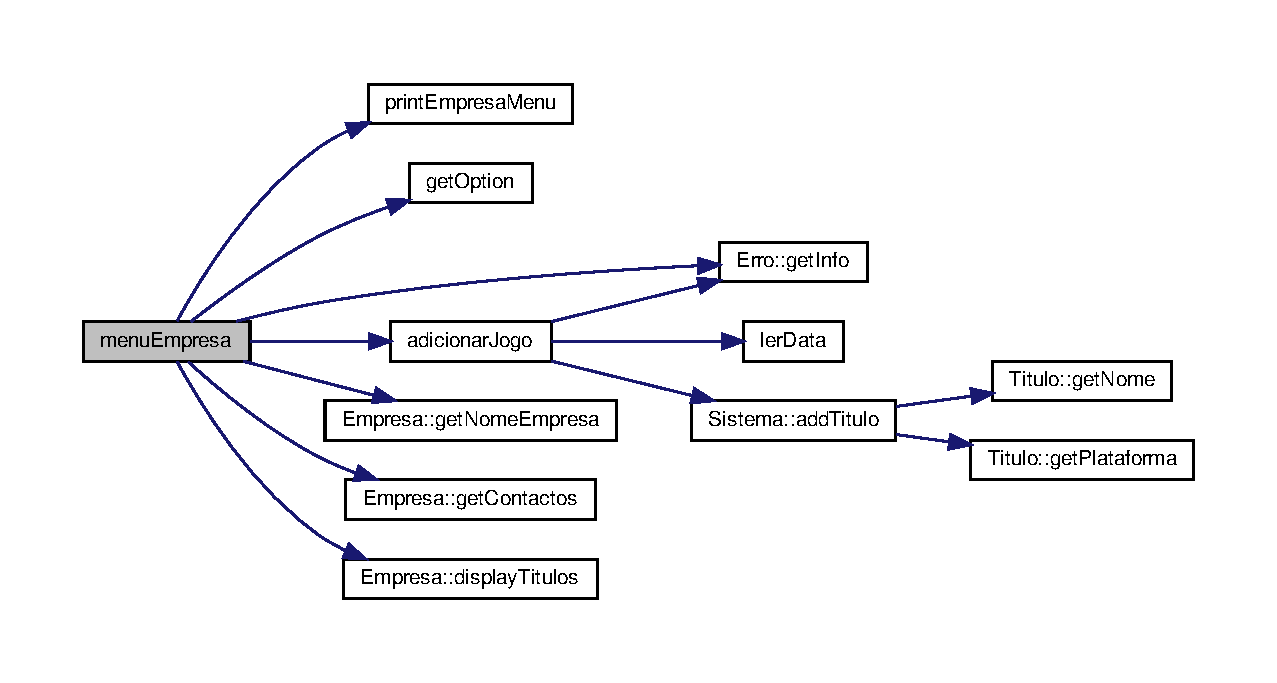
\includegraphics[width=350pt]{main_8cpp_a175192136cbe59d60bb80a1cd975fb68_cgraph}
\end{center}
\end{figure}
Here is the caller graph for this function\+:
\nopagebreak
\begin{figure}[H]
\begin{center}
\leavevmode
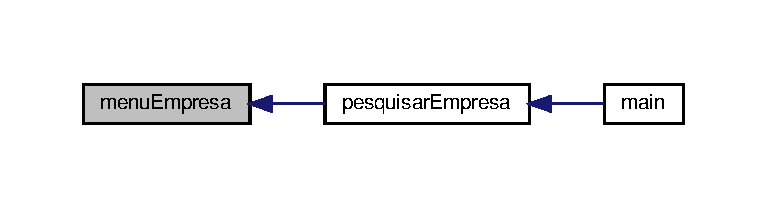
\includegraphics[width=350pt]{main_8cpp_a175192136cbe59d60bb80a1cd975fb68_icgraph}
\end{center}
\end{figure}
\mbox{\Hypertarget{main_8cpp_a41dd1ea1b95901e643be4af34f6dcfbf}\label{main_8cpp_a41dd1ea1b95901e643be4af34f6dcfbf}} 
\index{main.\+cpp@{main.\+cpp}!menu\+Utilizador@{menu\+Utilizador}}
\index{menu\+Utilizador@{menu\+Utilizador}!main.\+cpp@{main.\+cpp}}
\subsubsection{\texorpdfstring{menu\+Utilizador()}{menuUtilizador()}}
{\footnotesize\ttfamily void menu\+Utilizador (\begin{DoxyParamCaption}\item[{\hyperlink{classSistema}{Sistema} $\ast$}]{sistema,  }\item[{\hyperlink{classUtilizador}{Utilizador} $\ast$}]{u }\end{DoxyParamCaption})}


\begin{DoxyCode}
872                                                       \{
873     u->\hyperlink{classUtilizador_a4f3016ff86d68d548f801aa569b854dc}{printPublicidade}();
874     \textcolor{keywordtype}{int} opt;
875 
876     \textcolor{keywordflow}{while} (\textcolor{keyword}{true}) \{
877         \hyperlink{main_8cpp_a1b2cb3eb63cb3b95f68b994271b23f13}{printUserMenu}();
878 
879         \textcolor{keywordflow}{try} \{
880             opt = \hyperlink{main_8cpp_a69864162453f9299380c3c91be8fdca4}{getOption}(1, 9);
881         \} \textcolor{keywordflow}{catch} (\hyperlink{classInputInvalido}{InputInvalido} &e) \{
882             std::cout << \textcolor{stringliteral}{"\(\backslash\)n"} << e.\hyperlink{classErro_abfc1e9735b259d88bb97828a23164eb0}{getInfo}();
883             \textcolor{keywordflow}{continue};
884         \}
885 
886         \textcolor{keywordflow}{if} (opt == 1)
887             \hyperlink{main_8cpp_af8f302c02e726f24c5f7ddea9cd7f17d}{escolheTitulo}(sistema, u);
888         \textcolor{keywordflow}{else} \textcolor{keywordflow}{if} (opt == 2)
889             \hyperlink{main_8cpp_a11ccc3a4082cb5f294bc863d50fa803e}{adiconaWishlist}(sistema,u);
890         \textcolor{keywordflow}{else} \textcolor{keywordflow}{if} (opt == 3)
891             \hyperlink{main_8cpp_a01a46c12aa32213dc4babb7780904eba}{removerWishlist}(sistema,u);
892         \textcolor{keywordflow}{else} \textcolor{keywordflow}{if} (opt == 4)
893             \hyperlink{main_8cpp_aeeed8d2818f5d3d47c30b792b064f1d8}{alteraInteresse}(sistema,u);
894         \textcolor{keywordflow}{else} \textcolor{keywordflow}{if} (opt == 5)
895             \hyperlink{main_8cpp_aa59523879399e16bcfde4f06af6ad2ff}{escolheCc}(sistema, u);
896         \textcolor{keywordflow}{else} \textcolor{keywordflow}{if} (opt == 6)
897             sistema->\hyperlink{classSistema_aabeb8de1cc79bff9ff04d190ac3754d2}{saldoUtilizador}(u);
898         \textcolor{keywordflow}{else} \textcolor{keywordflow}{if} (opt == 7)
899             \hyperlink{main_8cpp_aab039f6f4271b56e9ca2d1264b25f66a}{utilizadorJoga}(sistema, u);
900         \textcolor{keywordflow}{else} \textcolor{keywordflow}{if} (opt == 8)
901             sistema->\hyperlink{classSistema_a871ba21f5de12adb05106f0fcaf9d723}{tempoJogado}(u);
902         \textcolor{keywordflow}{else}
903             \textcolor{keywordflow}{break};  \textcolor{comment}{// opt = 7, o utilizador quer sair}
904     \}
905 
906 \}
\end{DoxyCode}
Here is the call graph for this function\+:
\nopagebreak
\begin{figure}[H]
\begin{center}
\leavevmode
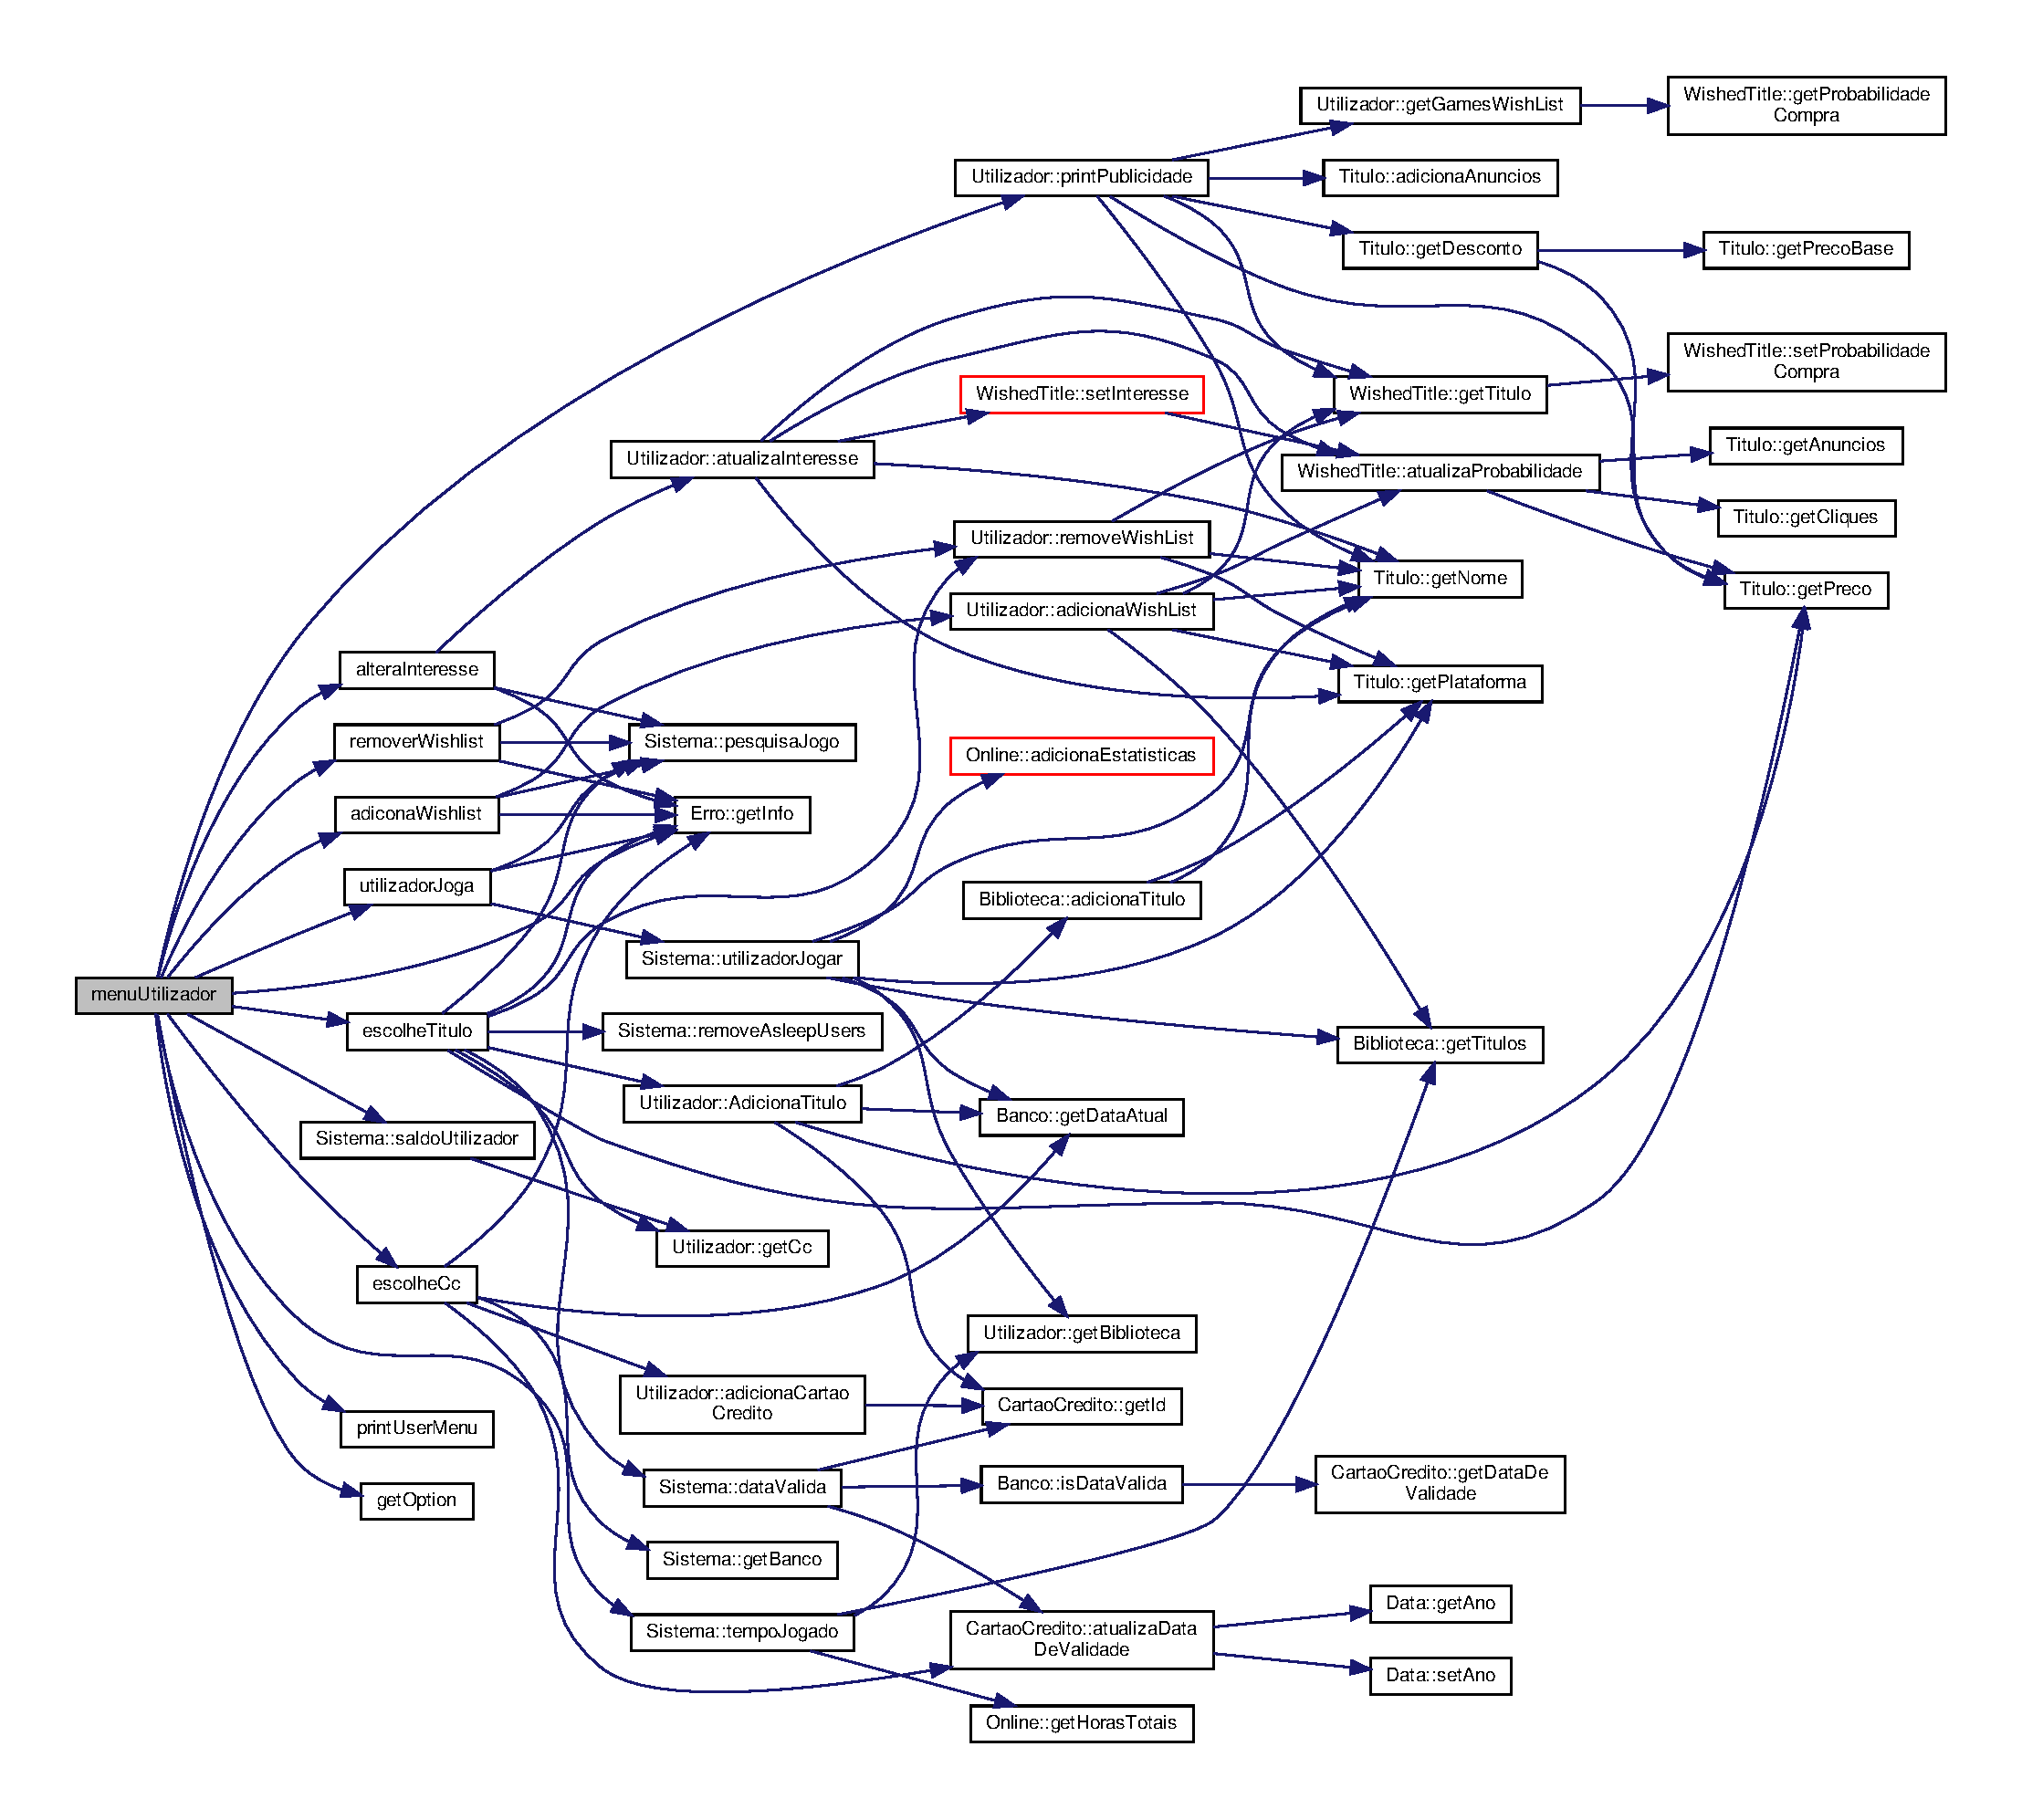
\includegraphics[width=350pt]{main_8cpp_a41dd1ea1b95901e643be4af34f6dcfbf_cgraph}
\end{center}
\end{figure}
Here is the caller graph for this function\+:
\nopagebreak
\begin{figure}[H]
\begin{center}
\leavevmode
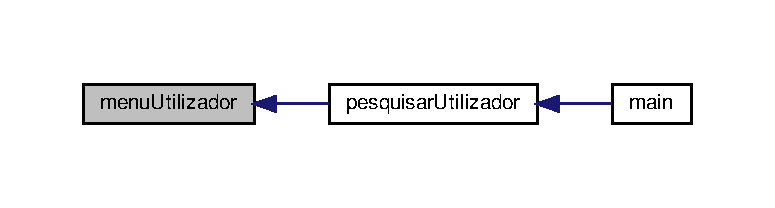
\includegraphics[width=350pt]{main_8cpp_a41dd1ea1b95901e643be4af34f6dcfbf_icgraph}
\end{center}
\end{figure}
\mbox{\Hypertarget{main_8cpp_aec6f563871c737f7e128ea66836a2be5}\label{main_8cpp_aec6f563871c737f7e128ea66836a2be5}} 
\index{main.\+cpp@{main.\+cpp}!ordena\+Jogos\+Utilizador@{ordena\+Jogos\+Utilizador}}
\index{ordena\+Jogos\+Utilizador@{ordena\+Jogos\+Utilizador}!main.\+cpp@{main.\+cpp}}
\subsubsection{\texorpdfstring{ordena\+Jogos\+Utilizador()}{ordenaJogosUtilizador()}}
{\footnotesize\ttfamily void ordena\+Jogos\+Utilizador (\begin{DoxyParamCaption}\item[{\hyperlink{classSistema}{Sistema} $\ast$}]{sistema,  }\item[{\hyperlink{classUtilizador}{Utilizador} $\ast$}]{u }\end{DoxyParamCaption})}


\begin{DoxyCode}
438                                                              \{
439     \textcolor{keywordtype}{int} opt;
440     std::vector<Titulo *> titulos;
441 
442     \textcolor{comment}{// Perguntar ao utilizador o que quer fazer at� este indicar que deseja sair}
443     \textcolor{keywordflow}{while} (\textcolor{keyword}{true}) \{
444         \hyperlink{main_8cpp_a6afc9271571dfdc7288faf87e9616e7d}{printDisplayTitulosMenu}();
445 
446         \textcolor{comment}{// Pedir opcao ao utilizador e verificar se nao houve erro de input}
447         \textcolor{keywordflow}{try} \{
448             opt = \hyperlink{main_8cpp_a69864162453f9299380c3c91be8fdca4}{getOption}(1, 9);
449         \} \textcolor{keywordflow}{catch} (\hyperlink{classInputInvalido}{InputInvalido} &e) \{
450             std::cout << \textcolor{stringliteral}{"\(\backslash\)n"} << e.\hyperlink{classErro_abfc1e9735b259d88bb97828a23164eb0}{getInfo}();
451             \textcolor{keywordflow}{continue};   \textcolor{comment}{// Ir para o proximo loop , pedir nova opcao}
452         \}
453 
454         \textcolor{keywordflow}{if} (opt == 1)
455             titulos = sistema->\hyperlink{classSistema_aade841c0c281c63fe922834e228049cd}{ordenaTitulosUtilizador}(u, \textcolor{stringliteral}{"id"}, \textcolor{keyword}{true});
456         \textcolor{keywordflow}{else} \textcolor{keywordflow}{if} (opt == 2)
457             titulos = sistema->\hyperlink{classSistema_aade841c0c281c63fe922834e228049cd}{ordenaTitulosUtilizador}(u, \textcolor{stringliteral}{"id"}, \textcolor{keyword}{false});
458         \textcolor{keywordflow}{else} \textcolor{keywordflow}{if} (opt == 3)
459             titulos = sistema->\hyperlink{classSistema_aade841c0c281c63fe922834e228049cd}{ordenaTitulosUtilizador}(u, \textcolor{stringliteral}{"data"}, \textcolor{keyword}{true});
460         \textcolor{keywordflow}{else} \textcolor{keywordflow}{if} (opt == 4)
461             titulos = sistema->\hyperlink{classSistema_aade841c0c281c63fe922834e228049cd}{ordenaTitulosUtilizador}(u, \textcolor{stringliteral}{"data"}, \textcolor{keyword}{false});
462         \textcolor{keywordflow}{else} \textcolor{keywordflow}{if} (opt == 5)
463             titulos = sistema->\hyperlink{classSistema_aade841c0c281c63fe922834e228049cd}{ordenaTitulosUtilizador}(u, \textcolor{stringliteral}{"idade"}, \textcolor{keyword}{true});
464         \textcolor{keywordflow}{else} \textcolor{keywordflow}{if} (opt == 6)
465             titulos = sistema->\hyperlink{classSistema_aade841c0c281c63fe922834e228049cd}{ordenaTitulosUtilizador}(u, \textcolor{stringliteral}{"idade"}, \textcolor{keyword}{false});
466         \textcolor{keywordflow}{else} \textcolor{keywordflow}{if} (opt == 7)
467             titulos = sistema->\hyperlink{classSistema_aade841c0c281c63fe922834e228049cd}{ordenaTitulosUtilizador}(u, \textcolor{stringliteral}{"empresa"}, \textcolor{keyword}{true});
468         \textcolor{keywordflow}{else} \textcolor{keywordflow}{if} (opt == 8)
469             titulos = sistema->\hyperlink{classSistema_aade841c0c281c63fe922834e228049cd}{ordenaTitulosUtilizador}(u, \textcolor{stringliteral}{"empresa"}, \textcolor{keyword}{false});
470         \textcolor{keywordflow}{else}
471             \textcolor{keywordflow}{break};  \textcolor{comment}{// opt = 9, o utilizador quer sair}
472 
473         \textcolor{keywordflow}{for} (\textcolor{keyword}{const} \textcolor{keyword}{auto} & titulo : titulos)
474             std::cout << titulo->getNome() << std::endl;
475     \}
476 \}
\end{DoxyCode}
Here is the call graph for this function\+:
\nopagebreak
\begin{figure}[H]
\begin{center}
\leavevmode
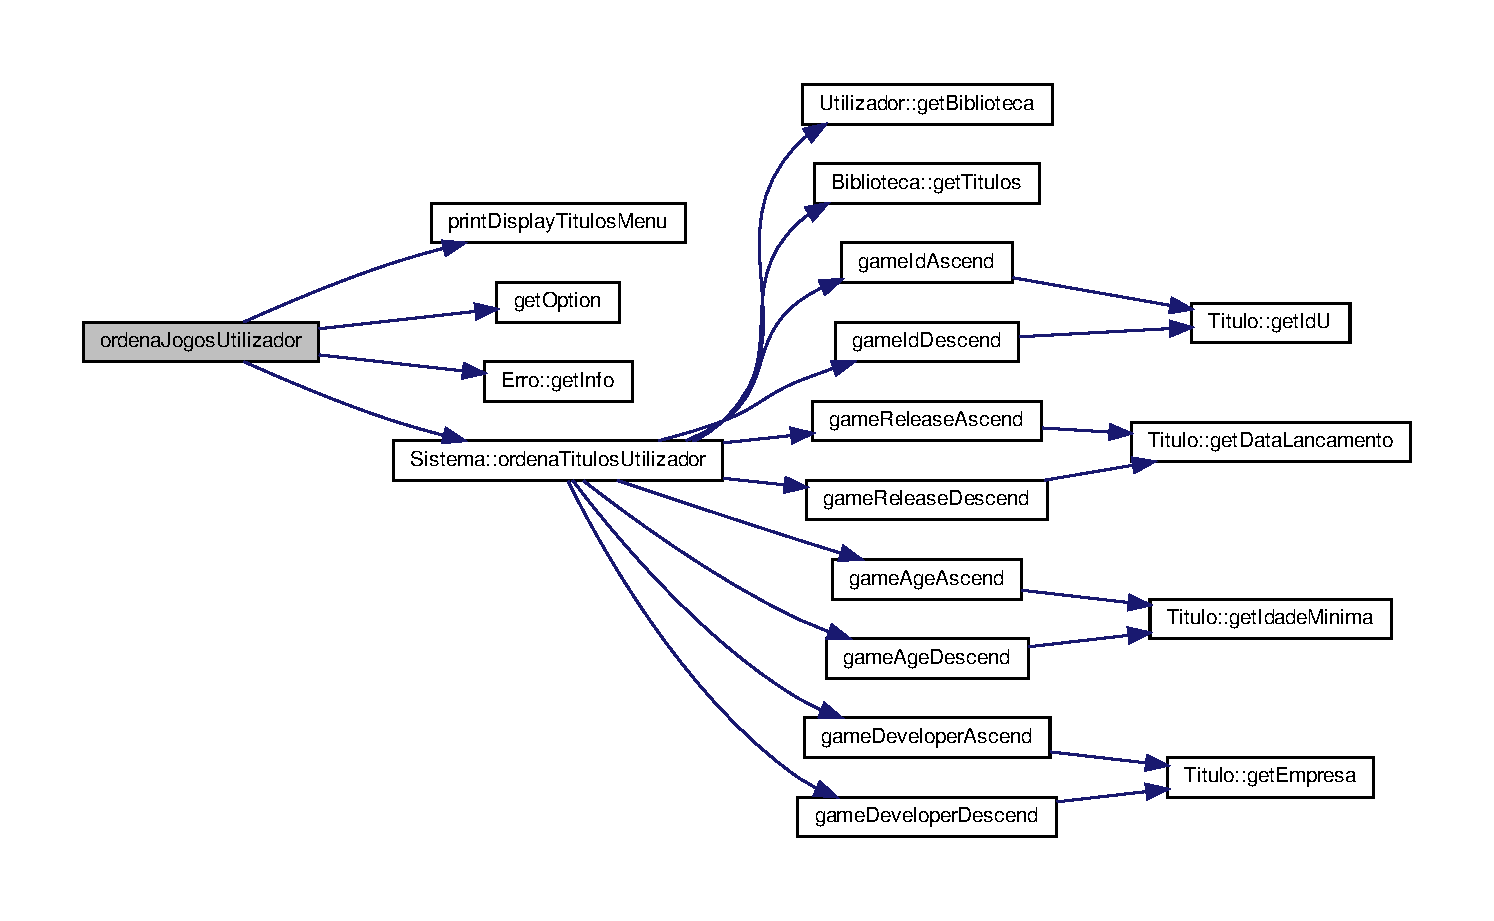
\includegraphics[width=350pt]{main_8cpp_aec6f563871c737f7e128ea66836a2be5_cgraph}
\end{center}
\end{figure}
\mbox{\Hypertarget{main_8cpp_ab5d3bc5e7f94dade3058f2afb385c8a4}\label{main_8cpp_ab5d3bc5e7f94dade3058f2afb385c8a4}} 
\index{main.\+cpp@{main.\+cpp}!pesquisar\+Empresa@{pesquisar\+Empresa}}
\index{pesquisar\+Empresa@{pesquisar\+Empresa}!main.\+cpp@{main.\+cpp}}
\subsubsection{\texorpdfstring{pesquisar\+Empresa()}{pesquisarEmpresa()}}
{\footnotesize\ttfamily void pesquisar\+Empresa (\begin{DoxyParamCaption}\item[{\hyperlink{classSistema}{Sistema} $\ast$}]{sistema }\end{DoxyParamCaption})}


\begin{DoxyCode}
987                                         \{
988     std::string nome;
989     std::string nif;
990 
991 
992     std::cout << std::endl << \textcolor{stringliteral}{"Nome da empresa: "};
993     getline(std::cin, nome);
994 
995     \textcolor{keywordflow}{while}(\textcolor{keyword}{true})\{
996         std::cout << \textcolor{stringliteral}{"Introduza o NIF: "};
997         getline(std::cin, nif);
998         \textcolor{keywordflow}{if}(\hyperlink{main_8cpp_a6c175a1424e435dba38c472eaf2f5535}{is\_digits}(nif) && nif.size()==9)\{
999             \textcolor{keywordflow}{break};
1000         \}
1001         \textcolor{keywordflow}{if}(nif.size()!=9)\{
1002             std::cout << \textcolor{stringliteral}{"Introduza um NIF com 9 digitos\(\backslash\)n"};
1003         \}
1004         \textcolor{keywordflow}{else} std::cout << \textcolor{stringliteral}{"O NIF so pode ter algarismos"};
1005     \}
1006 
1007     \textcolor{keywordflow}{try} \{
1008         \hyperlink{classEmpresa}{Empresa} *empresa=sistema->\hyperlink{classSistema_a1f22677c42afd48be088f2eca428dede}{pesquisaEmpresa}(nome,nif);
1009         \textcolor{keywordflow}{if}(empresa!=NULL)\{
1010             \hyperlink{main_8cpp_a175192136cbe59d60bb80a1cd975fb68}{menuEmpresa}(sistema, empresa);
1011         \}
1012     \} \textcolor{keywordflow}{catch} (\hyperlink{classEmpresaInexistente}{EmpresaInexistente} &e) \{
1013         std::cout << std::endl << e.\hyperlink{classErro_abfc1e9735b259d88bb97828a23164eb0}{getInfo}() << std::endl;
1014         \textcolor{keywordflow}{return};
1015     \}
1016 
1017 \}
\end{DoxyCode}
Here is the call graph for this function\+:
\nopagebreak
\begin{figure}[H]
\begin{center}
\leavevmode
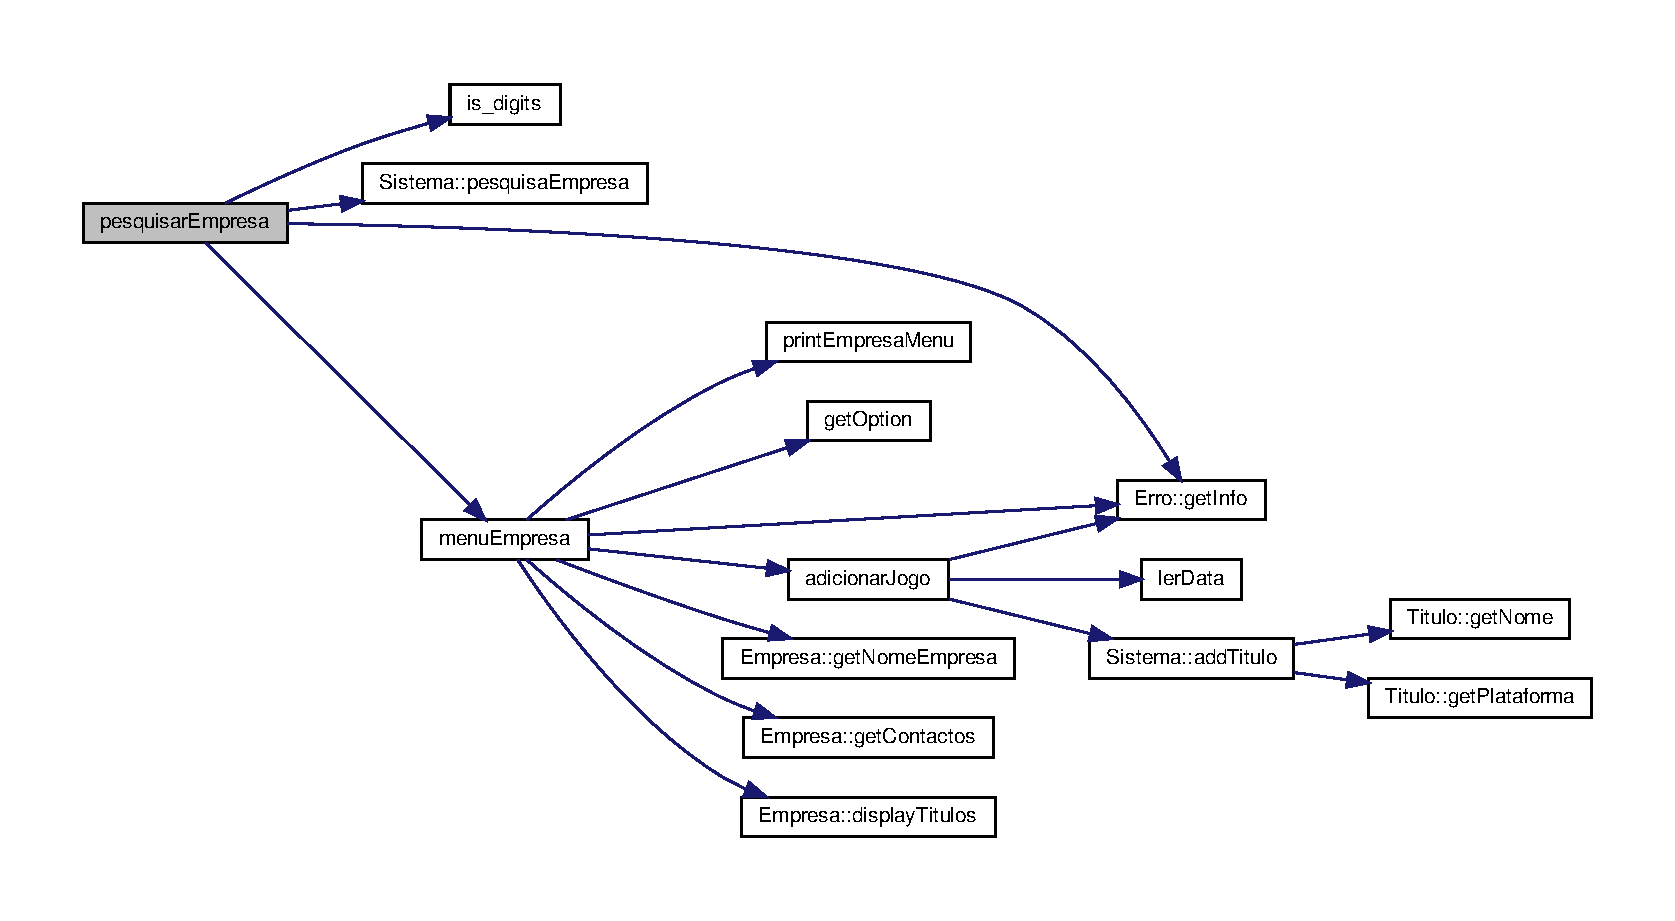
\includegraphics[width=350pt]{main_8cpp_ab5d3bc5e7f94dade3058f2afb385c8a4_cgraph}
\end{center}
\end{figure}
Here is the caller graph for this function\+:
\nopagebreak
\begin{figure}[H]
\begin{center}
\leavevmode
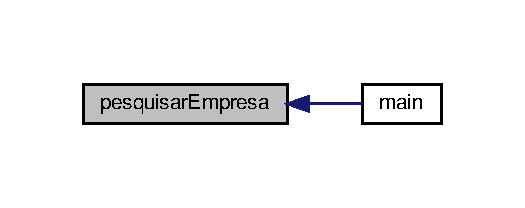
\includegraphics[width=252pt]{main_8cpp_ab5d3bc5e7f94dade3058f2afb385c8a4_icgraph}
\end{center}
\end{figure}
\mbox{\Hypertarget{main_8cpp_a84916567707f41d606bb5cbdd44d6c17}\label{main_8cpp_a84916567707f41d606bb5cbdd44d6c17}} 
\index{main.\+cpp@{main.\+cpp}!pesquisar\+Jogo@{pesquisar\+Jogo}}
\index{pesquisar\+Jogo@{pesquisar\+Jogo}!main.\+cpp@{main.\+cpp}}
\subsubsection{\texorpdfstring{pesquisar\+Jogo()}{pesquisarJogo()}}
{\footnotesize\ttfamily void pesquisar\+Jogo (\begin{DoxyParamCaption}\item[{\hyperlink{classSistema}{Sistema} $\ast$}]{sistema }\end{DoxyParamCaption})}


\begin{DoxyCode}
949                                       \{
950     std::string nome;
951     std::string plataforma;
952 
953 
954     std::cout << std::endl << \textcolor{stringliteral}{"Nome do titulo: "};
955     getline(std::cin, nome);
956 
957     std::cout << std::endl << \textcolor{stringliteral}{"Plataforma: "};
958     std::getline(std::cin, plataforma);
959 
960     \textcolor{keywordflow}{try} \{
961         \hyperlink{classTitulo}{Titulo} *t = sistema->\hyperlink{classSistema_a0fb81a4685bb24024295c89d22d6d719}{pesquisaJogo}(nome,plataforma);
962         t->\hyperlink{classTitulo_a0cf99e4a2b522a7acae425593e87efec}{adicionaCliques}(1);
963 
964         std::string atual;
965 
966             \hyperlink{classHome}{Home} * H = \textcolor{keyword}{dynamic\_cast<}\hyperlink{classHome}{Home} *\textcolor{keyword}{>}(t);
967             \textcolor{keywordflow}{if}(H!=NULL) \{
968             std::cout << \textcolor{stringliteral}{"Deseja adicionar uma atualizacao (dia atual) ('s' para processar uma atualizacao
       /outro para nao adicionar "}<<std::endl;
969             getline(std::cin,atual);
970             \textcolor{keywordflow}{if}(atual == \textcolor{stringliteral}{"s"}) \{
971                 H->\hyperlink{classHome_a94aec68b520d98ac38c6794b5771cd53}{adicionaAtualizacao}(sistema->\hyperlink{classSistema_abb768fdc8d4b8290ab4a267fc7a84a39}{getBanco}().
      \hyperlink{classBanco_a0735f07636c578666068a16f6ecccd91}{getDataAtual}());
972                 sistema->\hyperlink{classSistema_aa91f2955f6b47f4dc0523b86b94c6309}{adicionaAtualizacao}(nome,plataforma,sistema->
      \hyperlink{classSistema_abb768fdc8d4b8290ab4a267fc7a84a39}{getBanco}().\hyperlink{classBanco_a0735f07636c578666068a16f6ecccd91}{getDataAtual}());
973                 std::cout << \textcolor{stringliteral}{"Atualizacao bem sucedida para o respetivo titulo"}<<std::endl;
974 
975                 std::cout <<\textcolor{stringliteral}{"Atualizacoes existentes do titulo home"}<<std::endl;
976                 \textcolor{keywordflow}{for}(\textcolor{keyword}{const} \textcolor{keyword}{auto} &datas: H->\hyperlink{classHome_a0ab7279a76525f48cb1b64b8bae98a44}{getDatas}())
977                     std::cout << datas <<std::endl;
978             \}
979 
980             \}
981     \} \textcolor{keywordflow}{catch} (\hyperlink{classTituloInexistente}{TituloInexistente} &e) \{
982         std::cout << \textcolor{stringliteral}{"\(\backslash\)n"} << e.\hyperlink{classErro_abfc1e9735b259d88bb97828a23164eb0}{getInfo}();
983         \textcolor{keywordflow}{return};
984     \}
985 \}
\end{DoxyCode}
Here is the call graph for this function\+:
\nopagebreak
\begin{figure}[H]
\begin{center}
\leavevmode
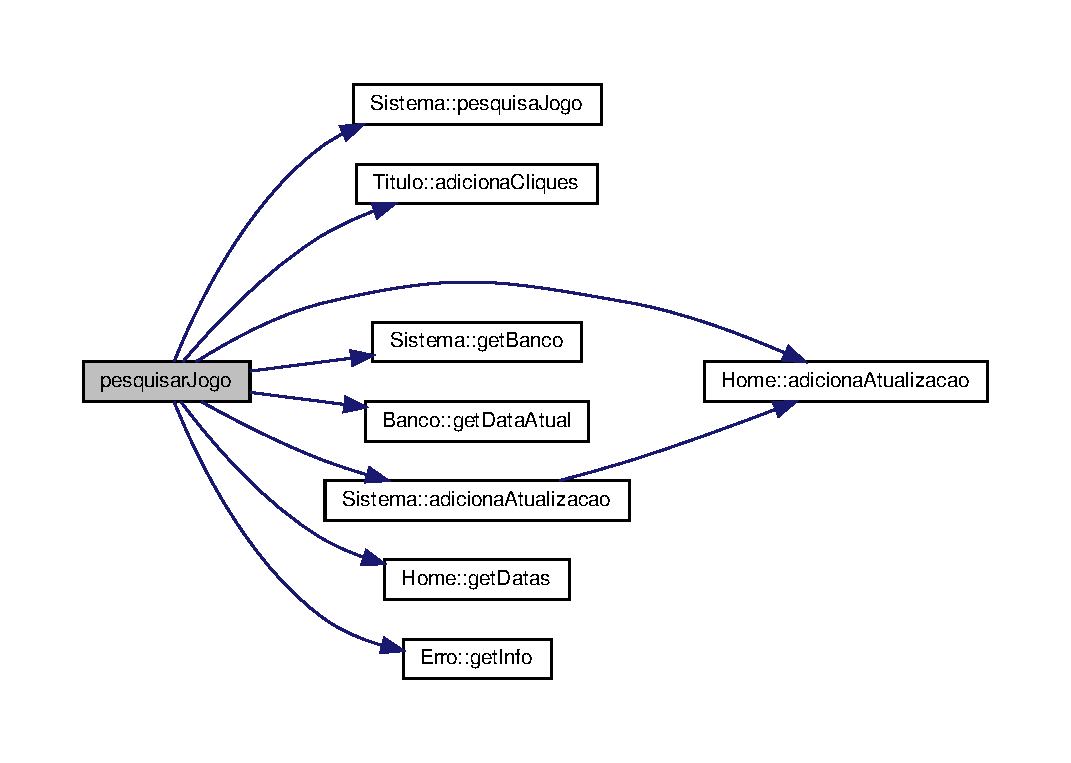
\includegraphics[width=350pt]{main_8cpp_a84916567707f41d606bb5cbdd44d6c17_cgraph}
\end{center}
\end{figure}
Here is the caller graph for this function\+:
\nopagebreak
\begin{figure}[H]
\begin{center}
\leavevmode
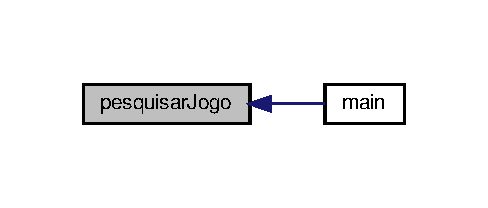
\includegraphics[width=234pt]{main_8cpp_a84916567707f41d606bb5cbdd44d6c17_icgraph}
\end{center}
\end{figure}
\mbox{\Hypertarget{main_8cpp_ab36c65bcfd56b6a29bee851e57462ad2}\label{main_8cpp_ab36c65bcfd56b6a29bee851e57462ad2}} 
\index{main.\+cpp@{main.\+cpp}!pesquisar\+Utilizador@{pesquisar\+Utilizador}}
\index{pesquisar\+Utilizador@{pesquisar\+Utilizador}!main.\+cpp@{main.\+cpp}}
\subsubsection{\texorpdfstring{pesquisar\+Utilizador()}{pesquisarUtilizador()}}
{\footnotesize\ttfamily void pesquisar\+Utilizador (\begin{DoxyParamCaption}\item[{\hyperlink{classSistema}{Sistema} $\ast$}]{sistema }\end{DoxyParamCaption})}


\begin{DoxyCode}
908                                             \{
909 
910     std::string nome;
911     std::cout << \textcolor{stringliteral}{"Insere o nome de um utilizador"} << std::endl;
912     getline(std::cin, nome);
913     std::string email;
914     std::string s;
915 
916     \textcolor{keywordflow}{while} (\textcolor{keyword}{true}) \{
917 
918         \textcolor{keywordflow}{while} (\textcolor{keyword}{true}) \{
919             \textcolor{keywordflow}{try} \{
920                 sistema->\hyperlink{classSistema_ac120f4aecf81933be110233f8dbf74c6}{isValidEmail}(email, \textcolor{keyword}{true});
921             \} \textcolor{keywordflow}{catch} (\hyperlink{classErro}{Erro} &e) \{
922                 std::cout << e.\hyperlink{classErro_abfc1e9735b259d88bb97828a23164eb0}{getInfo}() << std::endl;
923                 \textcolor{keywordflow}{continue};
924             \}
925             \textcolor{keywordflow}{break};
926         \}
927 
928         \textcolor{keywordflow}{try} \{
929             \hyperlink{classUtilizador}{Utilizador} *u = sistema->\hyperlink{classSistema_a6f2d2d67cb8464771272e60511045032}{pesquisaUtilizador}(nome, email);
930             \hyperlink{main_8cpp_a41dd1ea1b95901e643be4af34f6dcfbf}{menuUtilizador}(sistema, u);
931         \} \textcolor{keywordflow}{catch} (\hyperlink{classErro}{Erro} &e) \{
932             std::cout << e.\hyperlink{classErro_abfc1e9735b259d88bb97828a23164eb0}{getInfo}() << std::endl;
933             std::cout
934                     << \textcolor{stringliteral}{"Deseja desistir da procura('s' para sair/ outro para continuar)?"}
935                     << std::endl;
936             getline(std::cin, s);
937             \textcolor{keywordflow}{if} (s == \textcolor{stringliteral}{"s"})
938                 \textcolor{keywordflow}{return};
939 
940             std::cout << \textcolor{stringliteral}{"Insere o nome de um utilizador"} << std::endl;
941             getline(std::cin, nome);
942             \textcolor{keywordflow}{continue};
943         \}
944         \textcolor{keywordflow}{break};
945     \}
946 \}
\end{DoxyCode}
Here is the call graph for this function\+:
\nopagebreak
\begin{figure}[H]
\begin{center}
\leavevmode
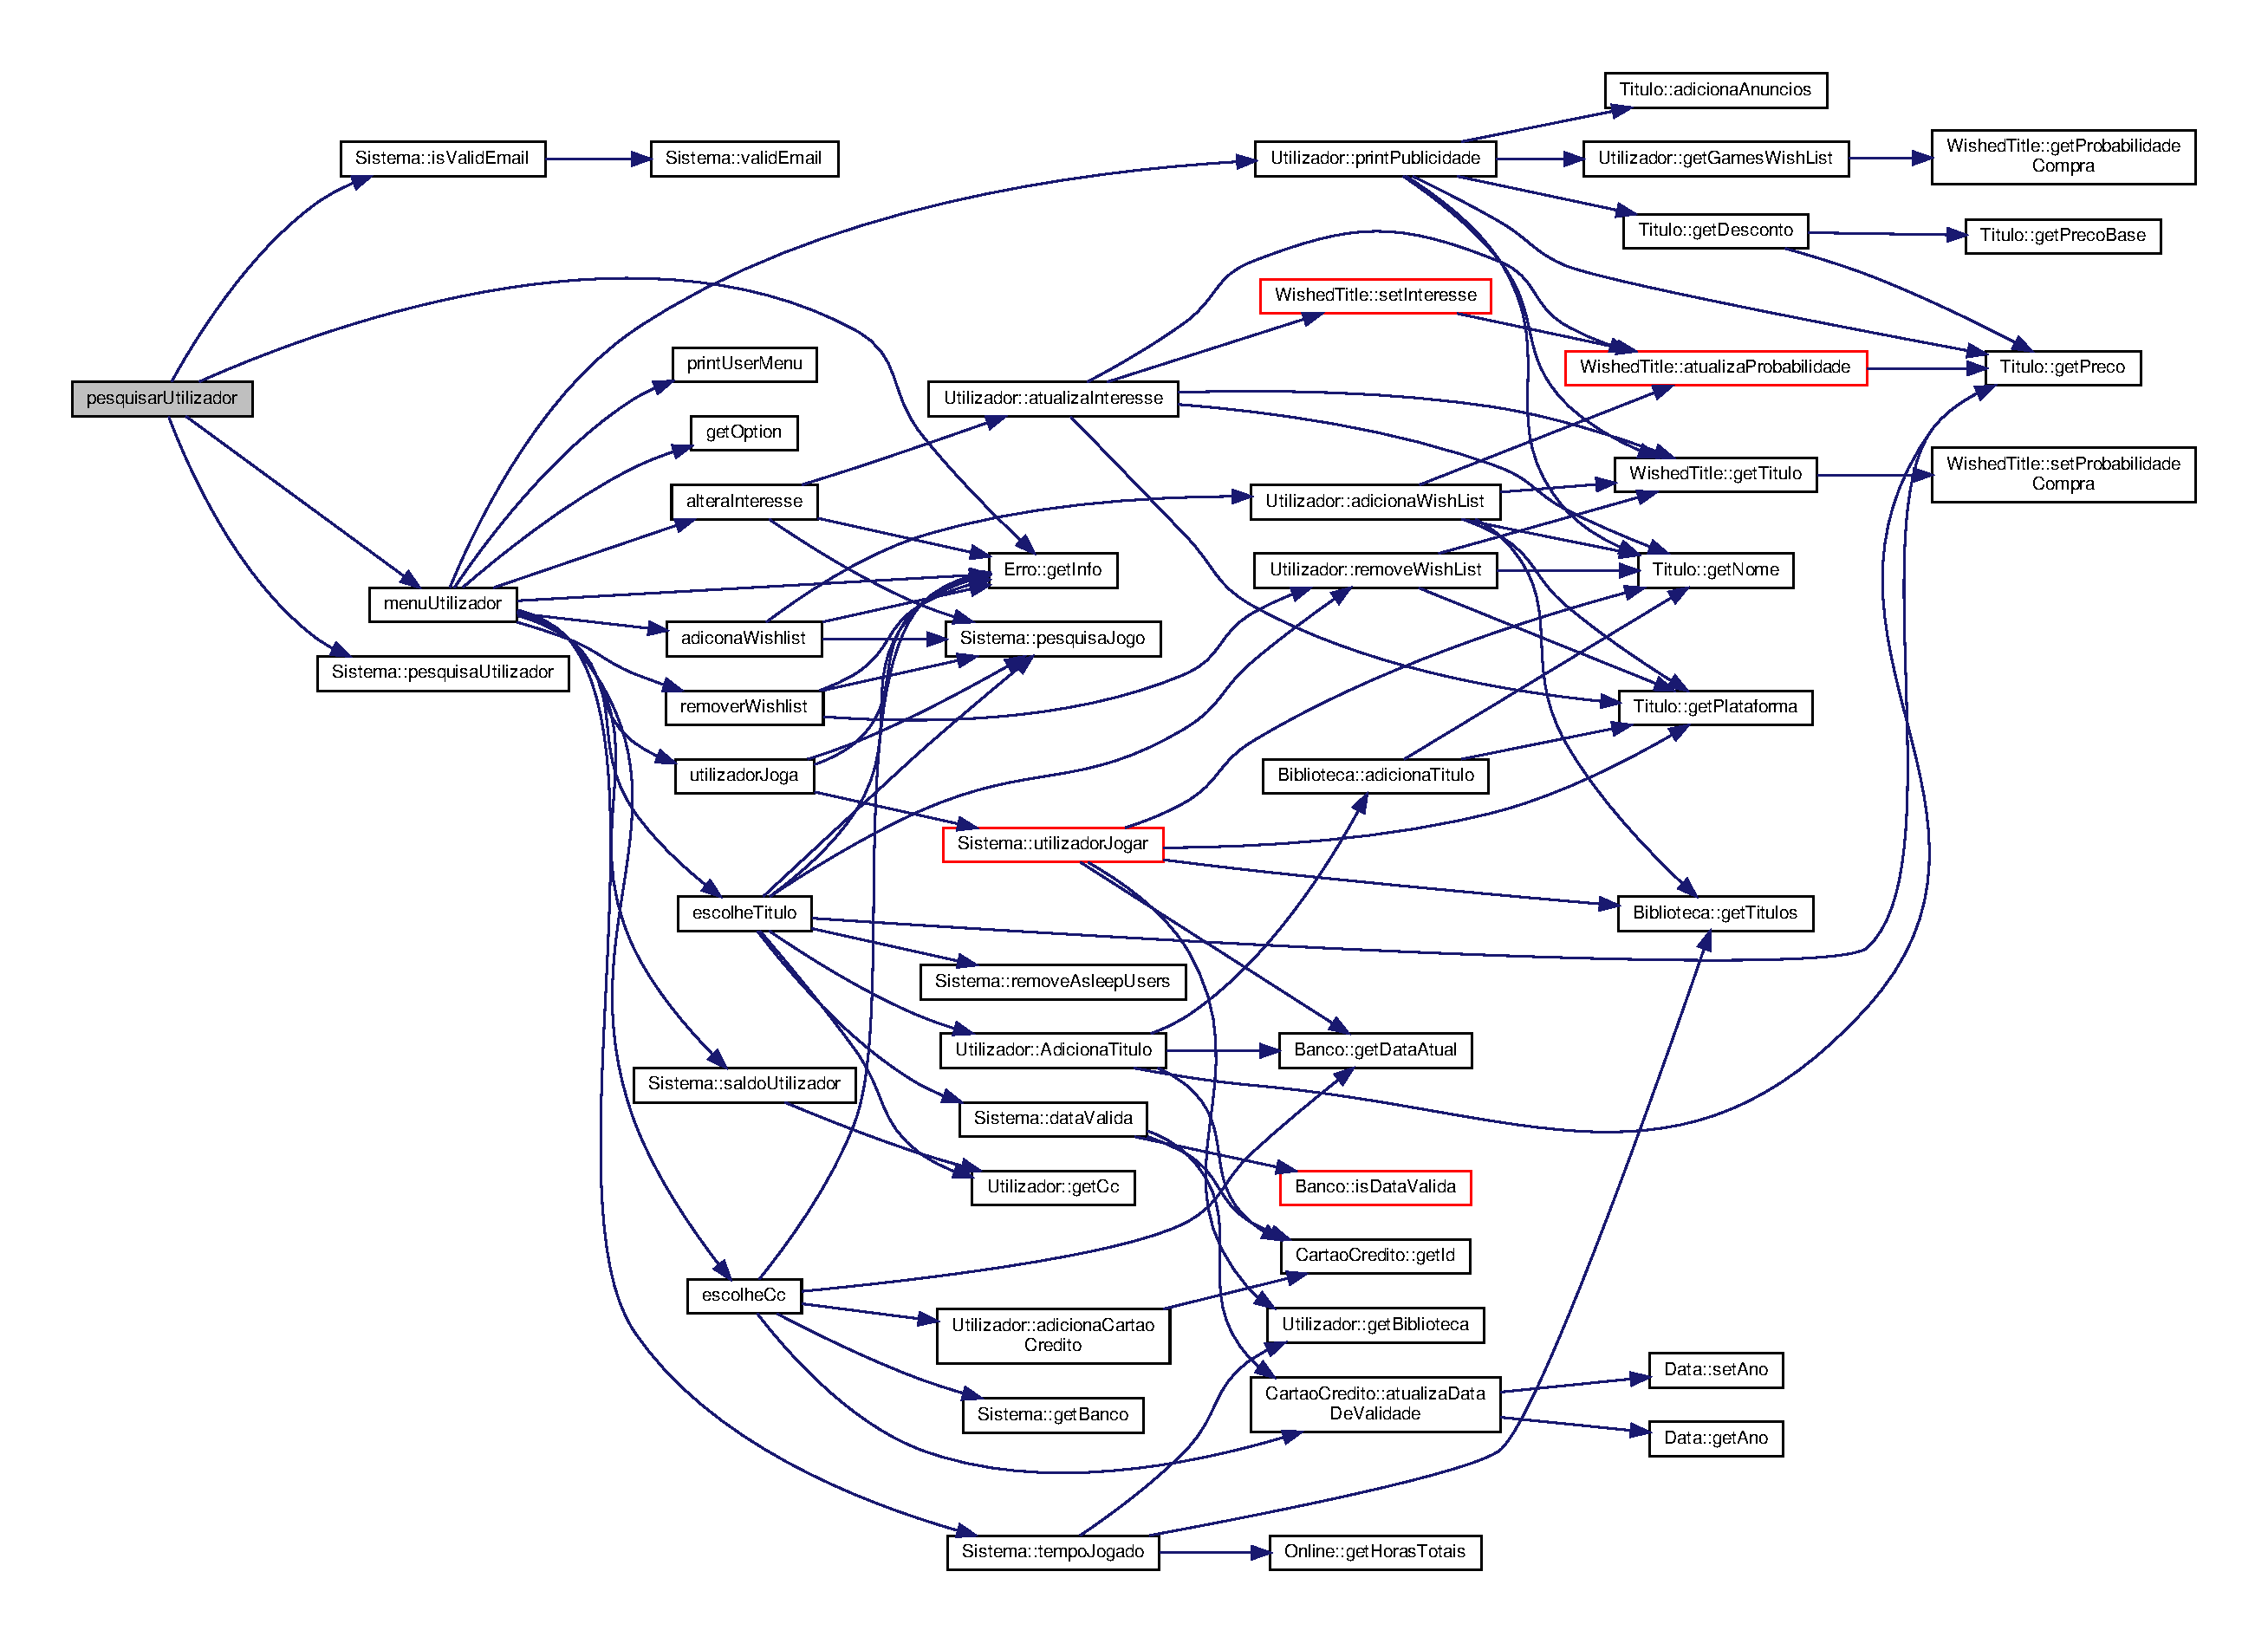
\includegraphics[width=350pt]{main_8cpp_ab36c65bcfd56b6a29bee851e57462ad2_cgraph}
\end{center}
\end{figure}
Here is the caller graph for this function\+:
\nopagebreak
\begin{figure}[H]
\begin{center}
\leavevmode
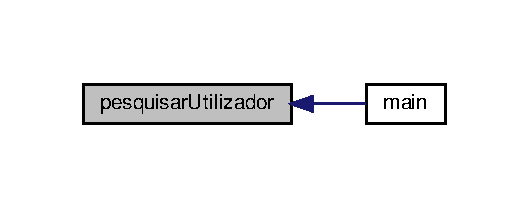
\includegraphics[width=254pt]{main_8cpp_ab36c65bcfd56b6a29bee851e57462ad2_icgraph}
\end{center}
\end{figure}
\mbox{\Hypertarget{main_8cpp_a9cdfd6b998ba8cfc497af7a303a6e330}\label{main_8cpp_a9cdfd6b998ba8cfc497af7a303a6e330}} 
\index{main.\+cpp@{main.\+cpp}!print\+Display\+Asleep\+Users\+Menu@{print\+Display\+Asleep\+Users\+Menu}}
\index{print\+Display\+Asleep\+Users\+Menu@{print\+Display\+Asleep\+Users\+Menu}!main.\+cpp@{main.\+cpp}}
\subsubsection{\texorpdfstring{print\+Display\+Asleep\+Users\+Menu()}{printDisplayAsleepUsersMenu()}}
{\footnotesize\ttfamily void print\+Display\+Asleep\+Users\+Menu (\begin{DoxyParamCaption}{ }\end{DoxyParamCaption})}


\begin{DoxyCode}
73                                   \{
74         \textcolor{comment}{// Draw the options}
75     std::cout << \textcolor{stringliteral}{"1. Visualizacao simples"} << std::endl;
76     std::cout << \textcolor{stringliteral}{"2. Para uma dada plataforma"} << std::endl;
77     std::cout << \textcolor{stringliteral}{"3. Para um dado titulo"} << std::endl;
78     std::cout << \textcolor{stringliteral}{"4. Para um dado genero"} << std::endl;
79     std::cout << \textcolor{stringliteral}{"5. Sair"} << std::endl << std::endl;
80 \}
\end{DoxyCode}
Here is the caller graph for this function\+:
\nopagebreak
\begin{figure}[H]
\begin{center}
\leavevmode
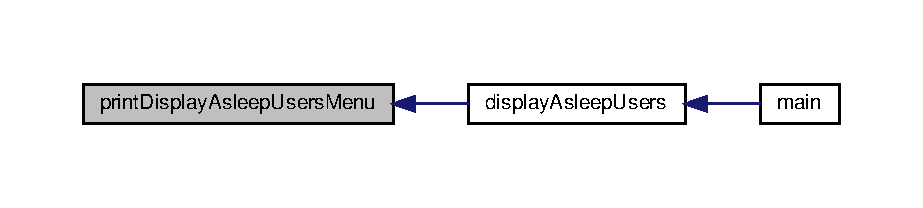
\includegraphics[width=350pt]{main_8cpp_a9cdfd6b998ba8cfc497af7a303a6e330_icgraph}
\end{center}
\end{figure}
\mbox{\Hypertarget{main_8cpp_a575a2b817f03c17e7943087813687578}\label{main_8cpp_a575a2b817f03c17e7943087813687578}} 
\index{main.\+cpp@{main.\+cpp}!print\+Display\+Empresas\+Menu@{print\+Display\+Empresas\+Menu}}
\index{print\+Display\+Empresas\+Menu@{print\+Display\+Empresas\+Menu}!main.\+cpp@{main.\+cpp}}
\subsubsection{\texorpdfstring{print\+Display\+Empresas\+Menu()}{printDisplayEmpresasMenu()}}
{\footnotesize\ttfamily void print\+Display\+Empresas\+Menu (\begin{DoxyParamCaption}{ }\end{DoxyParamCaption})}


\begin{DoxyCode}
64                                \{
65         \textcolor{comment}{// Draw the options}
66     std::cout << \textcolor{stringliteral}{"1. Visualizacao simples"} << std::endl;
67     std::cout << \textcolor{stringliteral}{"2. Titulos numa dada plataforma"} << std::endl;
68     std::cout << \textcolor{stringliteral}{"3. Numero de Titulos"} << std::endl;
69     std::cout << \textcolor{stringliteral}{"4. Titulos com um dado genero"} << std::endl;
70     std::cout << \textcolor{stringliteral}{"5. Sair"} << std::endl << std::endl;
71 \}
\end{DoxyCode}
Here is the caller graph for this function\+:
\nopagebreak
\begin{figure}[H]
\begin{center}
\leavevmode
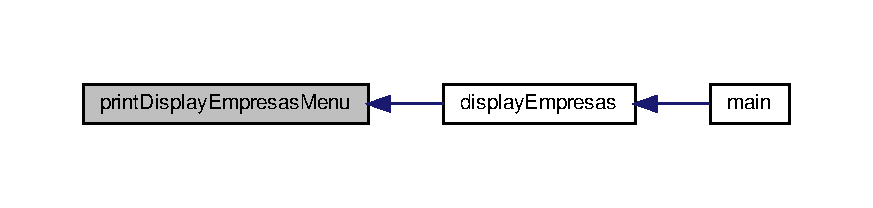
\includegraphics[width=350pt]{main_8cpp_a575a2b817f03c17e7943087813687578_icgraph}
\end{center}
\end{figure}
\mbox{\Hypertarget{main_8cpp_a6afc9271571dfdc7288faf87e9616e7d}\label{main_8cpp_a6afc9271571dfdc7288faf87e9616e7d}} 
\index{main.\+cpp@{main.\+cpp}!print\+Display\+Titulos\+Menu@{print\+Display\+Titulos\+Menu}}
\index{print\+Display\+Titulos\+Menu@{print\+Display\+Titulos\+Menu}!main.\+cpp@{main.\+cpp}}
\subsubsection{\texorpdfstring{print\+Display\+Titulos\+Menu()}{printDisplayTitulosMenu()}}
{\footnotesize\ttfamily void print\+Display\+Titulos\+Menu (\begin{DoxyParamCaption}{ }\end{DoxyParamCaption})}


\begin{DoxyCode}
124                                \{
125     \textcolor{comment}{// Draw the options}
126     std::cout << \textcolor{stringliteral}{"1. Visualizacao simples"} << std::endl;
127     std::cout << \textcolor{stringliteral}{"2. Data de lancamento crescente"} << std::endl;
128     std::cout << \textcolor{stringliteral}{"3. Data de lancamento decrescente"} << std::endl;
129     std::cout << \textcolor{stringliteral}{"4. Idade minima crescente"} << std::endl;
130     std::cout << \textcolor{stringliteral}{"5. Idade minima decrescente"} << std::endl;
131     std::cout << \textcolor{stringliteral}{"6. Empresa ordem alfabetica crescente"} << std::endl;
132     std::cout << \textcolor{stringliteral}{"7. Empresa ordem alfabetica decrescente"} << std::endl;
133     std::cout << \textcolor{stringliteral}{"8. Sair"} << std::endl << std::endl;
134 \}
\end{DoxyCode}
Here is the caller graph for this function\+:
\nopagebreak
\begin{figure}[H]
\begin{center}
\leavevmode
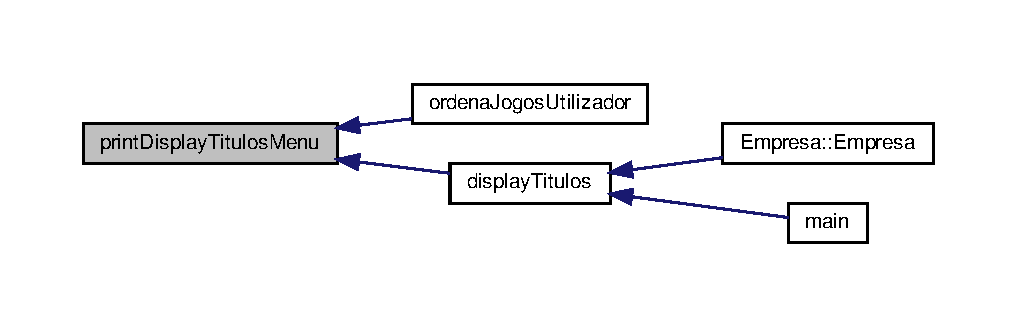
\includegraphics[width=350pt]{main_8cpp_a6afc9271571dfdc7288faf87e9616e7d_icgraph}
\end{center}
\end{figure}
\mbox{\Hypertarget{main_8cpp_a3687e2ced7dee82b39fc1ed74674ecd5}\label{main_8cpp_a3687e2ced7dee82b39fc1ed74674ecd5}} 
\index{main.\+cpp@{main.\+cpp}!print\+Display\+Utilizadores\+Menu@{print\+Display\+Utilizadores\+Menu}}
\index{print\+Display\+Utilizadores\+Menu@{print\+Display\+Utilizadores\+Menu}!main.\+cpp@{main.\+cpp}}
\subsubsection{\texorpdfstring{print\+Display\+Utilizadores\+Menu()}{printDisplayUtilizadoresMenu()}}
{\footnotesize\ttfamily void print\+Display\+Utilizadores\+Menu (\begin{DoxyParamCaption}{ }\end{DoxyParamCaption})}


\begin{DoxyCode}
97                                     \{
98 
99     \textcolor{comment}{// Draw the options}
100     std::cout << \textcolor{stringliteral}{"1. Visualizacao simples"} << std::endl;
101     std::cout << \textcolor{stringliteral}{"2. Idade crescente"} << std::endl;
102     std::cout << \textcolor{stringliteral}{"3. Idade decrescente"} << std::endl;
103     std::cout << \textcolor{stringliteral}{"4. Numero jogos crescente"} << std::endl;
104     std::cout << \textcolor{stringliteral}{"5. Numero de jogos descresnte"} << std::endl;
105     std::cout << \textcolor{stringliteral}{"6. Nome crescente"} << std::endl;
106     std::cout << \textcolor{stringliteral}{"7. Nome Decrescente"} << std::endl;
107     std::cout << \textcolor{stringliteral}{"8. Sair"} << std::endl << std::endl;
108 \}
\end{DoxyCode}
Here is the caller graph for this function\+:
\nopagebreak
\begin{figure}[H]
\begin{center}
\leavevmode
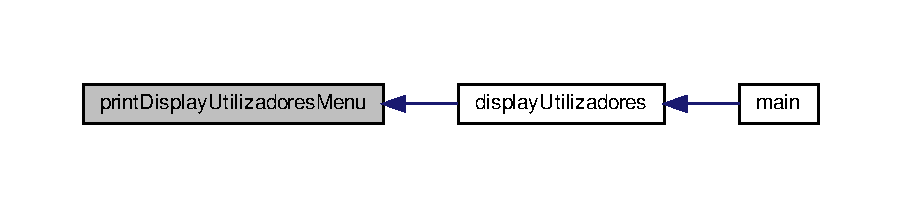
\includegraphics[width=350pt]{main_8cpp_a3687e2ced7dee82b39fc1ed74674ecd5_icgraph}
\end{center}
\end{figure}
\mbox{\Hypertarget{main_8cpp_a28b549948b369d4db7a926ec0cfd6e77}\label{main_8cpp_a28b549948b369d4db7a926ec0cfd6e77}} 
\index{main.\+cpp@{main.\+cpp}!print\+Empresa\+Menu@{print\+Empresa\+Menu}}
\index{print\+Empresa\+Menu@{print\+Empresa\+Menu}!main.\+cpp@{main.\+cpp}}
\subsubsection{\texorpdfstring{print\+Empresa\+Menu()}{printEmpresaMenu()}}
{\footnotesize\ttfamily void print\+Empresa\+Menu (\begin{DoxyParamCaption}{ }\end{DoxyParamCaption})}


\begin{DoxyCode}
838                         \{
839     \textcolor{comment}{// Draw the options}
840     std::cout << \textcolor{stringliteral}{"1. Adicionar titulo"} << std::endl;
841     std::cout << \textcolor{stringliteral}{"2. Visualizar contactos"} << std::endl;
842     std::cout << \textcolor{stringliteral}{"3. Visualizar titulos"} << std::endl;
843     std::cout << \textcolor{stringliteral}{"4. Sair"} << std::endl;
844 \}
\end{DoxyCode}
Here is the caller graph for this function\+:
\nopagebreak
\begin{figure}[H]
\begin{center}
\leavevmode
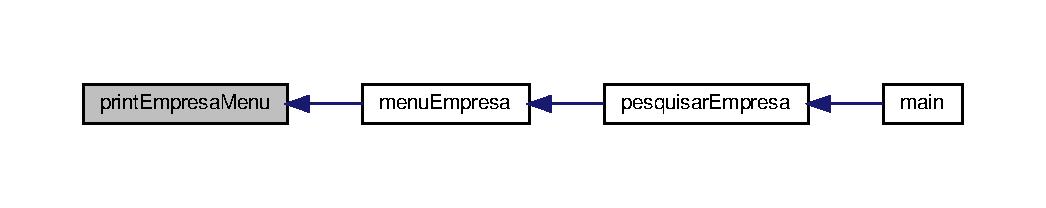
\includegraphics[width=350pt]{main_8cpp_a28b549948b369d4db7a926ec0cfd6e77_icgraph}
\end{center}
\end{figure}
\mbox{\Hypertarget{main_8cpp_af9dce1973196a5934ee5ec20ea417324}\label{main_8cpp_af9dce1973196a5934ee5ec20ea417324}} 
\index{main.\+cpp@{main.\+cpp}!print\+Main\+Menu@{print\+Main\+Menu}}
\index{print\+Main\+Menu@{print\+Main\+Menu}!main.\+cpp@{main.\+cpp}}
\subsubsection{\texorpdfstring{print\+Main\+Menu()}{printMainMenu()}}
{\footnotesize\ttfamily void print\+Main\+Menu (\begin{DoxyParamCaption}{ }\end{DoxyParamCaption})}


\begin{DoxyCode}
82                      \{
83 
84     std::cout << \textcolor{stringliteral}{"1. Visualizar Titulos"} << std::endl;
85     std::cout << \textcolor{stringliteral}{"2. Adicionar Utilizador"} << std::endl;
86     std::cout << \textcolor{stringliteral}{"3. Visualizar Utilizadores"} << std::endl;
87     std::cout << \textcolor{stringliteral}{"4. Pesquisar Utilizador"} << std::endl;
88     std::cout << \textcolor{stringliteral}{"5. Pesquisar Jogo"} << std::endl;
89     std::cout << \textcolor{stringliteral}{"6. Rankings e Estatisticas"} << std::endl;
90     std::cout << \textcolor{stringliteral}{"7. Adicionar Empresa"} << std::endl;
91     std::cout << \textcolor{stringliteral}{"8. Pesquisar Empresa"} << std::endl;
92     std::cout << \textcolor{stringliteral}{"9. Visualizar Empresas"} << std::endl;
93     std::cout << \textcolor{stringliteral}{"10. Visualizar Utilizadores Adormecidos"} << std::endl;
94     std::cout << \textcolor{stringliteral}{"11. Sair"} << std::endl << std::endl;
95 \}
\end{DoxyCode}
Here is the caller graph for this function\+:
\nopagebreak
\begin{figure}[H]
\begin{center}
\leavevmode
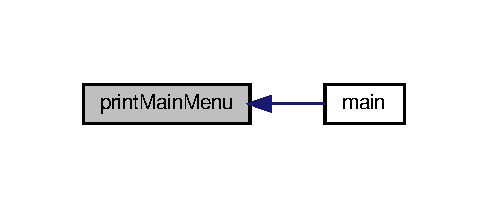
\includegraphics[width=234pt]{main_8cpp_af9dce1973196a5934ee5ec20ea417324_icgraph}
\end{center}
\end{figure}
\mbox{\Hypertarget{main_8cpp_a3da8cb0d6e5160fb3cf923a352965ff4}\label{main_8cpp_a3da8cb0d6e5160fb3cf923a352965ff4}} 
\index{main.\+cpp@{main.\+cpp}!print\+Ranking\+Menu@{print\+Ranking\+Menu}}
\index{print\+Ranking\+Menu@{print\+Ranking\+Menu}!main.\+cpp@{main.\+cpp}}
\subsubsection{\texorpdfstring{print\+Ranking\+Menu()}{printRankingMenu()}}
{\footnotesize\ttfamily void print\+Ranking\+Menu (\begin{DoxyParamCaption}{ }\end{DoxyParamCaption})}


\begin{DoxyCode}
1020 \{
1021     \textcolor{comment}{// Draw the options}
1022     std::cout << \textcolor{stringliteral}{"1. Ranking de Generos"} << std::endl;
1023     std::cout << \textcolor{stringliteral}{"2. Ranking de Idades"} << std::endl;
1024     std::cout << \textcolor{stringliteral}{"3. ranking de plataformas"} << std::endl;
1025     std::cout << \textcolor{stringliteral}{"4. Ranking de rentabilidade"} << std::endl;
1026     std::cout << \textcolor{stringliteral}{"5. Custo medio das bibliotecas"} << std::endl;
1027     std::cout << \textcolor{stringliteral}{"6. Numero medio de titulos das bibliotecas"} << std::endl;
1028     std::cout << \textcolor{stringliteral}{"7. Sair"} << std::endl;
1029 \}
\end{DoxyCode}
Here is the caller graph for this function\+:
\nopagebreak
\begin{figure}[H]
\begin{center}
\leavevmode
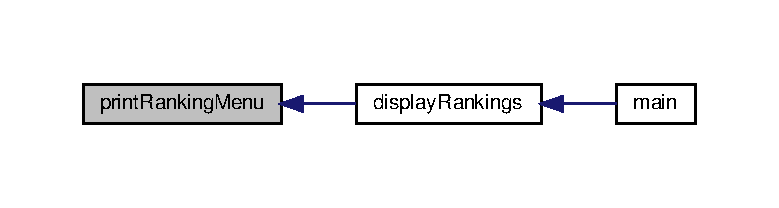
\includegraphics[width=350pt]{main_8cpp_a3da8cb0d6e5160fb3cf923a352965ff4_icgraph}
\end{center}
\end{figure}
\mbox{\Hypertarget{main_8cpp_a1b2cb3eb63cb3b95f68b994271b23f13}\label{main_8cpp_a1b2cb3eb63cb3b95f68b994271b23f13}} 
\index{main.\+cpp@{main.\+cpp}!print\+User\+Menu@{print\+User\+Menu}}
\index{print\+User\+Menu@{print\+User\+Menu}!main.\+cpp@{main.\+cpp}}
\subsubsection{\texorpdfstring{print\+User\+Menu()}{printUserMenu()}}
{\footnotesize\ttfamily void print\+User\+Menu (\begin{DoxyParamCaption}{ }\end{DoxyParamCaption})}


\begin{DoxyCode}
110                      \{
111 
112     \textcolor{comment}{// Draw the options}
113     std::cout << \textcolor{stringliteral}{"1. Adicionar titulo"} << std::endl;
114     std::cout << \textcolor{stringliteral}{"2. Adicionar titulo a whishlist"} << std::endl;
115     std::cout << \textcolor{stringliteral}{"3. Remover titulo da wishlsit"} << std::endl;
116     std::cout << \textcolor{stringliteral}{"4. Alterar interesse de jogo da wishlist"} << std::endl;
117     std::cout << \textcolor{stringliteral}{"5. Adicionar cartao de credito"} << std::endl;
118     std::cout << \textcolor{stringliteral}{"6. Verificar Saldo"} << std::endl;
119     std::cout << \textcolor{stringliteral}{"7. Jogar"} << std::endl;
120     std::cout << \textcolor{stringliteral}{"8. Tempo Jogado"} << std::endl;
121     std::cout << \textcolor{stringliteral}{"9. Sair"} << std::endl;
122 \}
\end{DoxyCode}
Here is the caller graph for this function\+:
\nopagebreak
\begin{figure}[H]
\begin{center}
\leavevmode
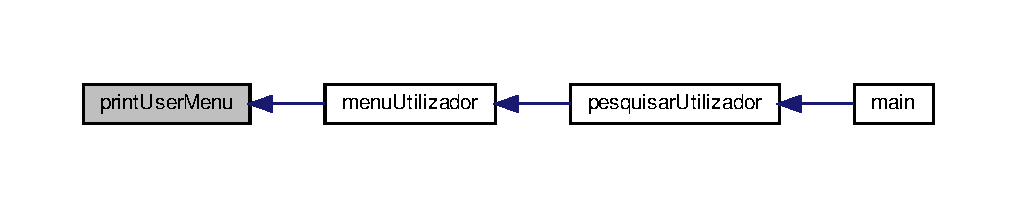
\includegraphics[width=350pt]{main_8cpp_a1b2cb3eb63cb3b95f68b994271b23f13_icgraph}
\end{center}
\end{figure}
\mbox{\Hypertarget{main_8cpp_a89a9bf7f76b270a3a9fc783b4009586c}\label{main_8cpp_a89a9bf7f76b270a3a9fc783b4009586c}} 
\index{main.\+cpp@{main.\+cpp}!print\+Welcome\+Menu@{print\+Welcome\+Menu}}
\index{print\+Welcome\+Menu@{print\+Welcome\+Menu}!main.\+cpp@{main.\+cpp}}
\subsubsection{\texorpdfstring{print\+Welcome\+Menu()}{printWelcomeMenu()}}
{\footnotesize\ttfamily void print\+Welcome\+Menu (\begin{DoxyParamCaption}{ }\end{DoxyParamCaption})}


\begin{DoxyCode}
35                         \{
36     \textcolor{keywordtype}{unsigned} \textcolor{keywordtype}{int} headerSize = 80;
37     std::string welcomeMessage = \textcolor{stringliteral}{"BIBLIOTECA DE JOGOS"};
38 
39     \textcolor{comment}{// Escrever uma mensagem de bem-vindo}
40     \textcolor{keywordflow}{for} (\textcolor{keywordtype}{unsigned} \textcolor{keywordtype}{int} i = 0; i < headerSize; i++) \{
41         std::cout << \textcolor{charliteral}{'-'};
42     \}
43     std::cout << std::endl;
44     \textcolor{keywordflow}{for} (\textcolor{keywordtype}{unsigned} \textcolor{keywordtype}{int} i = 0; i < headerSize; i++) \{
45         std::cout << \textcolor{charliteral}{'-'};
46     \}
47     std::cout << std::endl << std::endl;
48     \textcolor{keywordflow}{for} (\textcolor{keywordtype}{unsigned} \textcolor{keywordtype}{int} i = 0; i < (headerSize - welcomeMessage.size()) / 2;
49             i++) \{
50         std::cout << \textcolor{charliteral}{' '};
51     \}
52     std::cout << welcomeMessage << std::endl << std::endl;
53     \textcolor{keywordflow}{for} (\textcolor{keywordtype}{unsigned} \textcolor{keywordtype}{int} i = 0; i < headerSize; i++) \{
54         std::cout << \textcolor{charliteral}{'-'};
55     \}
56     std::cout << std::endl;
57     \textcolor{keywordflow}{for} (\textcolor{keywordtype}{unsigned} \textcolor{keywordtype}{int} i = 0; i < headerSize; i++) \{
58         std::cout << \textcolor{charliteral}{'-'};
59     \}
60     std::cout << std::endl << std::endl;
61 \}
\end{DoxyCode}
Here is the caller graph for this function\+:
\nopagebreak
\begin{figure}[H]
\begin{center}
\leavevmode
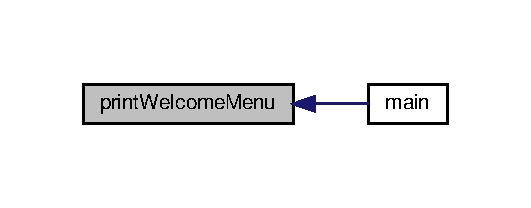
\includegraphics[width=255pt]{main_8cpp_a89a9bf7f76b270a3a9fc783b4009586c_icgraph}
\end{center}
\end{figure}
\mbox{\Hypertarget{main_8cpp_a01a46c12aa32213dc4babb7780904eba}\label{main_8cpp_a01a46c12aa32213dc4babb7780904eba}} 
\index{main.\+cpp@{main.\+cpp}!remover\+Wishlist@{remover\+Wishlist}}
\index{remover\+Wishlist@{remover\+Wishlist}!main.\+cpp@{main.\+cpp}}
\subsubsection{\texorpdfstring{remover\+Wishlist()}{removerWishlist()}}
{\footnotesize\ttfamily void remover\+Wishlist (\begin{DoxyParamCaption}\item[{\hyperlink{classSistema}{Sistema} $\ast$}]{sistema,  }\item[{\hyperlink{classUtilizador}{Utilizador} $\ast$}]{u }\end{DoxyParamCaption})}


\begin{DoxyCode}
664                                                      \{
665     std::string titulo;
666     std::string plataforma;
667     std::string s;
668     \textcolor{keywordtype}{bool} removed;
669 
670     \textcolor{keywordflow}{while} (\textcolor{keyword}{true}) \{
671         std::cout << \textcolor{stringliteral}{"Insira o nome do titulo"} << std::endl;
672         getline(std::cin, titulo);
673         std::cout << \textcolor{stringliteral}{"Insira a plataforma"} << std::endl;
674         getline(std::cin, plataforma);
675 
676         \textcolor{keywordflow}{try} \{
677             \hyperlink{classTitulo}{Titulo} * t = sistema->\hyperlink{classSistema_a0fb81a4685bb24024295c89d22d6d719}{pesquisaJogo}(titulo, plataforma);
678             removed = u->\hyperlink{classUtilizador_aa47c2fe835a73a23664149ccc7fbc10f}{removeWishList}(t);
679         \} \textcolor{keywordflow}{catch} (\hyperlink{classErro}{Erro} &e) \{
680             std::cout << e.\hyperlink{classErro_abfc1e9735b259d88bb97828a23164eb0}{getInfo}() << std::endl;
681             std::cout
682                     << \textcolor{stringliteral}{"Deseja desistir da procura('s' para sair/ outro para continuar)?"}
683                     << std::endl;
684             getline(std::cin, s);
685             \textcolor{keywordflow}{if} (s == \textcolor{stringliteral}{"s"})
686                 \textcolor{keywordflow}{return};
687 
688             \textcolor{keywordflow}{continue};
689         \}
690         \textcolor{keywordflow}{if}(!removed)\{
691             std::cout << \textcolor{stringliteral}{"Titulo inexistente na wishlist"}<<std::endl;
692             std::cout
693                     << \textcolor{stringliteral}{"Deseja desistir da procura('s' para sair/ outro para continuar)?"}
694                     << std::endl;
695             getline(std::cin, s);
696             \textcolor{keywordflow}{if} (s == \textcolor{stringliteral}{"s"})
697                 \textcolor{keywordflow}{return};
698 
699             \textcolor{keywordflow}{continue};
700         \}
701         std::cout << \textcolor{stringliteral}{"Jogo removido com sucesso!"} << std::endl;
702         \textcolor{keywordflow}{break};
703     \}
704 \}
\end{DoxyCode}
Here is the call graph for this function\+:
\nopagebreak
\begin{figure}[H]
\begin{center}
\leavevmode
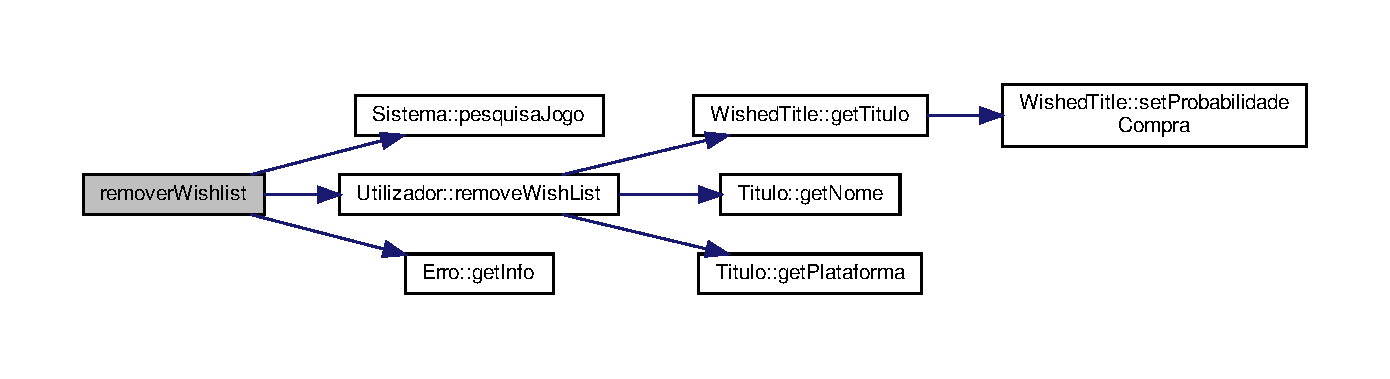
\includegraphics[width=350pt]{main_8cpp_a01a46c12aa32213dc4babb7780904eba_cgraph}
\end{center}
\end{figure}
Here is the caller graph for this function\+:
\nopagebreak
\begin{figure}[H]
\begin{center}
\leavevmode
\includegraphics[width=350pt]{main_8cpp_a01a46c12aa32213dc4babb7780904eba_icgraph}
\end{center}
\end{figure}
\mbox{\Hypertarget{main_8cpp_aab039f6f4271b56e9ca2d1264b25f66a}\label{main_8cpp_aab039f6f4271b56e9ca2d1264b25f66a}} 
\index{main.\+cpp@{main.\+cpp}!utilizador\+Joga@{utilizador\+Joga}}
\index{utilizador\+Joga@{utilizador\+Joga}!main.\+cpp@{main.\+cpp}}
\subsubsection{\texorpdfstring{utilizador\+Joga()}{utilizadorJoga()}}
{\footnotesize\ttfamily void utilizador\+Joga (\begin{DoxyParamCaption}\item[{\hyperlink{classSistema}{Sistema} $\ast$}]{sistema,  }\item[{\hyperlink{classUtilizador}{Utilizador} $\ast$}]{u }\end{DoxyParamCaption})}


\begin{DoxyCode}
783                                                       \{
784     std::string titulo;
785     std::string plataforma;
786     std::string s;
787     \hyperlink{classTitulo}{Titulo} * t;
788 
789     \textcolor{keywordflow}{while} (\textcolor{keyword}{true}) \{
790         std::cout << \textcolor{stringliteral}{"Insira o nome do titulo"} << std::endl;
791         getline(std::cin, titulo);
792         std::cout << \textcolor{stringliteral}{"Insira a plataforma"} << std::endl;
793         getline(std::cin, plataforma);
794 
795         \textcolor{keywordflow}{try} \{
796             t = sistema->\hyperlink{classSistema_a0fb81a4685bb24024295c89d22d6d719}{pesquisaJogo}(titulo, plataforma);
797 
798             \textcolor{keywordflow}{if} (dynamic\_cast<Online *>(t) == NULL) \{
799                 std::cout << \textcolor{stringliteral}{"Nao e um titulo online!"} << std::endl;
800 
801                 std::cout
802                         << \textcolor{stringliteral}{"Deseja desistir da procura('s' para sair/ outro para continuar)?"}
803                         << std::endl;
804                 getline(std::cin, s);
805                 \textcolor{keywordflow}{if} (s == \textcolor{stringliteral}{"s"})
806                     \textcolor{keywordflow}{return};
807 
808                 \textcolor{keywordflow}{continue};
809             \}
810         \} \textcolor{keywordflow}{catch} (\hyperlink{classErro}{Erro} &e) \{
811             std::cout << e.\hyperlink{classErro_abfc1e9735b259d88bb97828a23164eb0}{getInfo}() << std::endl;
812             std::cout
813                     << \textcolor{stringliteral}{"Deseja desistir da procura('s' para sair/ outro para continuar)?"}
814                     << std::endl;
815             getline(std::cin, s);
816             \textcolor{keywordflow}{if} (s == \textcolor{stringliteral}{"s"})
817                 \textcolor{keywordflow}{return};
818 
819             \textcolor{keywordflow}{continue};
820         \}
821         \textcolor{keywordflow}{break};
822     \}
823 
824     std::cout << \textcolor{stringliteral}{"Numero de minutos a jogar:"} << std::endl;
825     \textcolor{keywordtype}{int} n;
826     std::cin >> n;
827     \textcolor{keywordflow}{if} (!std::cin) \textcolor{comment}{// or if(cin.fail())}
828     \{
829         \textcolor{comment}{// user didn't input a number}
830         std::cin.clear(); \textcolor{comment}{// reset failbit}
831         std::cin.ignore(std::numeric\_limits<std::streamsize>::max(), \textcolor{charliteral}{'\(\backslash\)n'}); \textcolor{comment}{//skip bad input}
832         std::cout << \textcolor{stringliteral}{"Numero de horas a jogar:"} << std::endl;
833     \}
834     sistema->\hyperlink{classSistema_a43e1d500eca075857b1c96c2e2239d55}{utilizadorJogar}(u, t, n);
835     std::cout << \textcolor{stringliteral}{"O utilizador jogou durante "} << n << \textcolor{stringliteral}{" minutos."} << std::endl;
836 \}
\end{DoxyCode}
Here is the call graph for this function\+:
\nopagebreak
\begin{figure}[H]
\begin{center}
\leavevmode
\includegraphics[width=350pt]{main_8cpp_aab039f6f4271b56e9ca2d1264b25f66a_cgraph}
\end{center}
\end{figure}
Here is the caller graph for this function\+:
\nopagebreak
\begin{figure}[H]
\begin{center}
\leavevmode
\includegraphics[width=350pt]{main_8cpp_aab039f6f4271b56e9ca2d1264b25f66a_icgraph}
\end{center}
\end{figure}

\hypertarget{_sistema_8cpp}{}\section{Sistema.\+cpp File Reference}
\label{_sistema_8cpp}\index{Sistema.\+cpp@{Sistema.\+cpp}}
{\ttfamily \#include \char`\"{}Sistema.\+h\char`\"{}}\newline
{\ttfamily \#include $<$utility$>$}\newline
{\ttfamily \#include $<$iostream$>$}\newline
{\ttfamily \#include $<$sstream$>$}\newline
{\ttfamily \#include $<$algorithm$>$}\newline
{\ttfamily \#include \char`\"{}Titulo.\+h\char`\"{}}\newline
{\ttfamily \#include $<$vector$>$}\newline
{\ttfamily \#include $<$cctype$>$}\newline
{\ttfamily \#include $<$cstring$>$}\newline
{\ttfamily \#include $<$queue$>$}\newline
Include dependency graph for Sistema.\+cpp\+:
% FIG 0
\subsection*{Functions}
\begin{DoxyCompactItemize}
\item 
bool \mbox{\hyperlink{_sistema_8cpp_a2cac2b30d054ab23d49adc954779f67d}{user\+Name\+Ascend}} (\mbox{\hyperlink{class_utilizador}{Utilizador}} $\ast$user1, \mbox{\hyperlink{class_utilizador}{Utilizador}} $\ast$user2)
\item 
bool \mbox{\hyperlink{_sistema_8cpp_ac0995133035c1bd2be3a18c95a2eba92}{user\+Name\+Descend}} (\mbox{\hyperlink{class_utilizador}{Utilizador}} $\ast$user1, \mbox{\hyperlink{class_utilizador}{Utilizador}} $\ast$user2)
\item 
bool \mbox{\hyperlink{_sistema_8cpp_ad518f0e0db218f2c049ef1d700caae5f}{user\+Age\+Ascend}} (\mbox{\hyperlink{class_utilizador}{Utilizador}} $\ast$user1, \mbox{\hyperlink{class_utilizador}{Utilizador}} $\ast$user2)
\item 
bool \mbox{\hyperlink{_sistema_8cpp_a02190b2d4dada73645956850b936ad16}{user\+Age\+Descend}} (\mbox{\hyperlink{class_utilizador}{Utilizador}} $\ast$user1, \mbox{\hyperlink{class_utilizador}{Utilizador}} $\ast$user2)
\item 
bool \mbox{\hyperlink{_sistema_8cpp_a55b7ab55cae2d4f6a03844e5cb19d2b8}{user\+Number\+Games\+Ascend}} (\mbox{\hyperlink{class_utilizador}{Utilizador}} $\ast$user1, \mbox{\hyperlink{class_utilizador}{Utilizador}} $\ast$user2)
\item 
bool \mbox{\hyperlink{_sistema_8cpp_a81e28a299272eebc9771023c1f78ea48}{user\+Number\+Games\+Descend}} (\mbox{\hyperlink{class_utilizador}{Utilizador}} $\ast$user1, \mbox{\hyperlink{class_utilizador}{Utilizador}} $\ast$user2)
\item 
bool \mbox{\hyperlink{_sistema_8cpp_a9ebb751fccefae6ee1c4636c901cf0bc}{game\+Id\+Ascend}} (\mbox{\hyperlink{class_titulo}{Titulo}} $\ast$titulo1, \mbox{\hyperlink{class_titulo}{Titulo}} $\ast$titulo2)
\item 
bool \mbox{\hyperlink{_sistema_8cpp_a5de4e871b807cfbcd024a00f60d18ba1}{game\+Id\+Descend}} (\mbox{\hyperlink{class_titulo}{Titulo}} $\ast$titulo1, \mbox{\hyperlink{class_titulo}{Titulo}} $\ast$titulo2)
\item 
bool \mbox{\hyperlink{_sistema_8cpp_a4b576dc41b8edeb29c8f84c948c47665}{game\+Release\+Ascend}} (\mbox{\hyperlink{class_titulo}{Titulo}} $\ast$titulo1, \mbox{\hyperlink{class_titulo}{Titulo}} $\ast$titulo2)
\item 
bool \mbox{\hyperlink{_sistema_8cpp_af8a401eaa3da373780504f34a1216550}{game\+Release\+Descend}} (\mbox{\hyperlink{class_titulo}{Titulo}} $\ast$titulo1, \mbox{\hyperlink{class_titulo}{Titulo}} $\ast$titulo2)
\item 
bool \mbox{\hyperlink{_sistema_8cpp_a85fca79d7efc04e9982238e38e199154}{game\+Age\+Ascend}} (\mbox{\hyperlink{class_titulo}{Titulo}} $\ast$titulo1, \mbox{\hyperlink{class_titulo}{Titulo}} $\ast$titulo2)
\item 
bool \mbox{\hyperlink{_sistema_8cpp_a4d0cdff5caed7ad707a1f6926e301a51}{game\+Age\+Descend}} (\mbox{\hyperlink{class_titulo}{Titulo}} $\ast$titulo1, \mbox{\hyperlink{class_titulo}{Titulo}} $\ast$titulo2)
\item 
bool \mbox{\hyperlink{_sistema_8cpp_ac71c10d662fb0c03358b94519364a76e}{game\+Developer\+Ascend}} (\mbox{\hyperlink{class_titulo}{Titulo}} $\ast$titulo1, \mbox{\hyperlink{class_titulo}{Titulo}} $\ast$titulo2)
\item 
bool \mbox{\hyperlink{_sistema_8cpp_a7ce8e20323381359eed30807d3dadabd}{game\+Developer\+Descend}} (\mbox{\hyperlink{class_titulo}{Titulo}} $\ast$titulo1, \mbox{\hyperlink{class_titulo}{Titulo}} $\ast$titulo2)
\item 
bool \mbox{\hyperlink{_sistema_8cpp_a3236be9bb24a1c78a5a87e45410380de}{cmp\+Par\+Jogo\+Rentabilidade}} (const std\+::pair$<$ std\+::string, float $>$ \&p1, const std\+::pair$<$ std\+::string, float $>$ \&p2)
\item 
void \mbox{\hyperlink{_sistema_8cpp_a9a4d5048551696a97f3dfff84b4d736d}{display\+Rank}} (std\+::vector$<$ std\+::string $>$ a)
\item 
int \mbox{\hyperlink{_sistema_8cpp_a466ff65ea754156e5bfa50747f1015b4}{find\+Pair}} (const std\+::vector$<$ std\+::pair$<$ std\+::string, float $>$$>$ \&rentabilidade, std\+::string nome)
\end{DoxyCompactItemize}


\subsection{Function Documentation}
\mbox{\Hypertarget{_sistema_8cpp_a3236be9bb24a1c78a5a87e45410380de}\label{_sistema_8cpp_a3236be9bb24a1c78a5a87e45410380de}} 
\index{Sistema.\+cpp@{Sistema.\+cpp}!cmp\+Par\+Jogo\+Rentabilidade@{cmp\+Par\+Jogo\+Rentabilidade}}
\index{cmp\+Par\+Jogo\+Rentabilidade@{cmp\+Par\+Jogo\+Rentabilidade}!Sistema.\+cpp@{Sistema.\+cpp}}
\subsubsection{\texorpdfstring{cmp\+Par\+Jogo\+Rentabilidade()}{cmpParJogoRentabilidade()}}
{\footnotesize\ttfamily bool cmp\+Par\+Jogo\+Rentabilidade (\begin{DoxyParamCaption}\item[{const std\+::pair$<$ std\+::string, float $>$ \&}]{p1,  }\item[{const std\+::pair$<$ std\+::string, float $>$ \&}]{p2 }\end{DoxyParamCaption})}

\mbox{\Hypertarget{_sistema_8cpp_a9a4d5048551696a97f3dfff84b4d736d}\label{_sistema_8cpp_a9a4d5048551696a97f3dfff84b4d736d}} 
\index{Sistema.\+cpp@{Sistema.\+cpp}!display\+Rank@{display\+Rank}}
\index{display\+Rank@{display\+Rank}!Sistema.\+cpp@{Sistema.\+cpp}}
\subsubsection{\texorpdfstring{display\+Rank()}{displayRank()}}
{\footnotesize\ttfamily void display\+Rank (\begin{DoxyParamCaption}\item[{std\+::vector$<$ std\+::string $>$}]{a }\end{DoxyParamCaption})}

\mbox{\Hypertarget{_sistema_8cpp_a466ff65ea754156e5bfa50747f1015b4}\label{_sistema_8cpp_a466ff65ea754156e5bfa50747f1015b4}} 
\index{Sistema.\+cpp@{Sistema.\+cpp}!find\+Pair@{find\+Pair}}
\index{find\+Pair@{find\+Pair}!Sistema.\+cpp@{Sistema.\+cpp}}
\subsubsection{\texorpdfstring{find\+Pair()}{findPair()}}
{\footnotesize\ttfamily int find\+Pair (\begin{DoxyParamCaption}\item[{const std\+::vector$<$ std\+::pair$<$ std\+::string, float $>$$>$ \&}]{rentabilidade,  }\item[{std\+::string}]{nome }\end{DoxyParamCaption})}

\mbox{\Hypertarget{_sistema_8cpp_a85fca79d7efc04e9982238e38e199154}\label{_sistema_8cpp_a85fca79d7efc04e9982238e38e199154}} 
\index{Sistema.\+cpp@{Sistema.\+cpp}!game\+Age\+Ascend@{game\+Age\+Ascend}}
\index{game\+Age\+Ascend@{game\+Age\+Ascend}!Sistema.\+cpp@{Sistema.\+cpp}}
\subsubsection{\texorpdfstring{game\+Age\+Ascend()}{gameAgeAscend()}}
{\footnotesize\ttfamily bool game\+Age\+Ascend (\begin{DoxyParamCaption}\item[{\mbox{\hyperlink{class_titulo}{Titulo}} $\ast$}]{titulo1,  }\item[{\mbox{\hyperlink{class_titulo}{Titulo}} $\ast$}]{titulo2 }\end{DoxyParamCaption})}

Here is the call graph for this function\+:
% FIG 1
\mbox{\Hypertarget{_sistema_8cpp_a4d0cdff5caed7ad707a1f6926e301a51}\label{_sistema_8cpp_a4d0cdff5caed7ad707a1f6926e301a51}} 
\index{Sistema.\+cpp@{Sistema.\+cpp}!game\+Age\+Descend@{game\+Age\+Descend}}
\index{game\+Age\+Descend@{game\+Age\+Descend}!Sistema.\+cpp@{Sistema.\+cpp}}
\subsubsection{\texorpdfstring{game\+Age\+Descend()}{gameAgeDescend()}}
{\footnotesize\ttfamily bool game\+Age\+Descend (\begin{DoxyParamCaption}\item[{\mbox{\hyperlink{class_titulo}{Titulo}} $\ast$}]{titulo1,  }\item[{\mbox{\hyperlink{class_titulo}{Titulo}} $\ast$}]{titulo2 }\end{DoxyParamCaption})}

Here is the call graph for this function\+:
% FIG 2
\mbox{\Hypertarget{_sistema_8cpp_ac71c10d662fb0c03358b94519364a76e}\label{_sistema_8cpp_ac71c10d662fb0c03358b94519364a76e}} 
\index{Sistema.\+cpp@{Sistema.\+cpp}!game\+Developer\+Ascend@{game\+Developer\+Ascend}}
\index{game\+Developer\+Ascend@{game\+Developer\+Ascend}!Sistema.\+cpp@{Sistema.\+cpp}}
\subsubsection{\texorpdfstring{game\+Developer\+Ascend()}{gameDeveloperAscend()}}
{\footnotesize\ttfamily bool game\+Developer\+Ascend (\begin{DoxyParamCaption}\item[{\mbox{\hyperlink{class_titulo}{Titulo}} $\ast$}]{titulo1,  }\item[{\mbox{\hyperlink{class_titulo}{Titulo}} $\ast$}]{titulo2 }\end{DoxyParamCaption})}

Here is the call graph for this function\+:
% FIG 3
\mbox{\Hypertarget{_sistema_8cpp_a7ce8e20323381359eed30807d3dadabd}\label{_sistema_8cpp_a7ce8e20323381359eed30807d3dadabd}} 
\index{Sistema.\+cpp@{Sistema.\+cpp}!game\+Developer\+Descend@{game\+Developer\+Descend}}
\index{game\+Developer\+Descend@{game\+Developer\+Descend}!Sistema.\+cpp@{Sistema.\+cpp}}
\subsubsection{\texorpdfstring{game\+Developer\+Descend()}{gameDeveloperDescend()}}
{\footnotesize\ttfamily bool game\+Developer\+Descend (\begin{DoxyParamCaption}\item[{\mbox{\hyperlink{class_titulo}{Titulo}} $\ast$}]{titulo1,  }\item[{\mbox{\hyperlink{class_titulo}{Titulo}} $\ast$}]{titulo2 }\end{DoxyParamCaption})}

Here is the call graph for this function\+:
% FIG 4
\mbox{\Hypertarget{_sistema_8cpp_a9ebb751fccefae6ee1c4636c901cf0bc}\label{_sistema_8cpp_a9ebb751fccefae6ee1c4636c901cf0bc}} 
\index{Sistema.\+cpp@{Sistema.\+cpp}!game\+Id\+Ascend@{game\+Id\+Ascend}}
\index{game\+Id\+Ascend@{game\+Id\+Ascend}!Sistema.\+cpp@{Sistema.\+cpp}}
\subsubsection{\texorpdfstring{game\+Id\+Ascend()}{gameIdAscend()}}
{\footnotesize\ttfamily bool game\+Id\+Ascend (\begin{DoxyParamCaption}\item[{\mbox{\hyperlink{class_titulo}{Titulo}} $\ast$}]{titulo1,  }\item[{\mbox{\hyperlink{class_titulo}{Titulo}} $\ast$}]{titulo2 }\end{DoxyParamCaption})}

Here is the call graph for this function\+:
% FIG 5
\mbox{\Hypertarget{_sistema_8cpp_a5de4e871b807cfbcd024a00f60d18ba1}\label{_sistema_8cpp_a5de4e871b807cfbcd024a00f60d18ba1}} 
\index{Sistema.\+cpp@{Sistema.\+cpp}!game\+Id\+Descend@{game\+Id\+Descend}}
\index{game\+Id\+Descend@{game\+Id\+Descend}!Sistema.\+cpp@{Sistema.\+cpp}}
\subsubsection{\texorpdfstring{game\+Id\+Descend()}{gameIdDescend()}}
{\footnotesize\ttfamily bool game\+Id\+Descend (\begin{DoxyParamCaption}\item[{\mbox{\hyperlink{class_titulo}{Titulo}} $\ast$}]{titulo1,  }\item[{\mbox{\hyperlink{class_titulo}{Titulo}} $\ast$}]{titulo2 }\end{DoxyParamCaption})}

Here is the call graph for this function\+:
% FIG 6
\mbox{\Hypertarget{_sistema_8cpp_a4b576dc41b8edeb29c8f84c948c47665}\label{_sistema_8cpp_a4b576dc41b8edeb29c8f84c948c47665}} 
\index{Sistema.\+cpp@{Sistema.\+cpp}!game\+Release\+Ascend@{game\+Release\+Ascend}}
\index{game\+Release\+Ascend@{game\+Release\+Ascend}!Sistema.\+cpp@{Sistema.\+cpp}}
\subsubsection{\texorpdfstring{game\+Release\+Ascend()}{gameReleaseAscend()}}
{\footnotesize\ttfamily bool game\+Release\+Ascend (\begin{DoxyParamCaption}\item[{\mbox{\hyperlink{class_titulo}{Titulo}} $\ast$}]{titulo1,  }\item[{\mbox{\hyperlink{class_titulo}{Titulo}} $\ast$}]{titulo2 }\end{DoxyParamCaption})}

Here is the call graph for this function\+:
% FIG 7
\mbox{\Hypertarget{_sistema_8cpp_af8a401eaa3da373780504f34a1216550}\label{_sistema_8cpp_af8a401eaa3da373780504f34a1216550}} 
\index{Sistema.\+cpp@{Sistema.\+cpp}!game\+Release\+Descend@{game\+Release\+Descend}}
\index{game\+Release\+Descend@{game\+Release\+Descend}!Sistema.\+cpp@{Sistema.\+cpp}}
\subsubsection{\texorpdfstring{game\+Release\+Descend()}{gameReleaseDescend()}}
{\footnotesize\ttfamily bool game\+Release\+Descend (\begin{DoxyParamCaption}\item[{\mbox{\hyperlink{class_titulo}{Titulo}} $\ast$}]{titulo1,  }\item[{\mbox{\hyperlink{class_titulo}{Titulo}} $\ast$}]{titulo2 }\end{DoxyParamCaption})}

Here is the call graph for this function\+:
% FIG 8
\mbox{\Hypertarget{_sistema_8cpp_ad518f0e0db218f2c049ef1d700caae5f}\label{_sistema_8cpp_ad518f0e0db218f2c049ef1d700caae5f}} 
\index{Sistema.\+cpp@{Sistema.\+cpp}!user\+Age\+Ascend@{user\+Age\+Ascend}}
\index{user\+Age\+Ascend@{user\+Age\+Ascend}!Sistema.\+cpp@{Sistema.\+cpp}}
\subsubsection{\texorpdfstring{user\+Age\+Ascend()}{userAgeAscend()}}
{\footnotesize\ttfamily bool user\+Age\+Ascend (\begin{DoxyParamCaption}\item[{\mbox{\hyperlink{class_utilizador}{Utilizador}} $\ast$}]{user1,  }\item[{\mbox{\hyperlink{class_utilizador}{Utilizador}} $\ast$}]{user2 }\end{DoxyParamCaption})}

Here is the call graph for this function\+:
% FIG 9
\mbox{\Hypertarget{_sistema_8cpp_a02190b2d4dada73645956850b936ad16}\label{_sistema_8cpp_a02190b2d4dada73645956850b936ad16}} 
\index{Sistema.\+cpp@{Sistema.\+cpp}!user\+Age\+Descend@{user\+Age\+Descend}}
\index{user\+Age\+Descend@{user\+Age\+Descend}!Sistema.\+cpp@{Sistema.\+cpp}}
\subsubsection{\texorpdfstring{user\+Age\+Descend()}{userAgeDescend()}}
{\footnotesize\ttfamily bool user\+Age\+Descend (\begin{DoxyParamCaption}\item[{\mbox{\hyperlink{class_utilizador}{Utilizador}} $\ast$}]{user1,  }\item[{\mbox{\hyperlink{class_utilizador}{Utilizador}} $\ast$}]{user2 }\end{DoxyParamCaption})}

Here is the call graph for this function\+:
% FIG 10
\mbox{\Hypertarget{_sistema_8cpp_a2cac2b30d054ab23d49adc954779f67d}\label{_sistema_8cpp_a2cac2b30d054ab23d49adc954779f67d}} 
\index{Sistema.\+cpp@{Sistema.\+cpp}!user\+Name\+Ascend@{user\+Name\+Ascend}}
\index{user\+Name\+Ascend@{user\+Name\+Ascend}!Sistema.\+cpp@{Sistema.\+cpp}}
\subsubsection{\texorpdfstring{user\+Name\+Ascend()}{userNameAscend()}}
{\footnotesize\ttfamily bool user\+Name\+Ascend (\begin{DoxyParamCaption}\item[{\mbox{\hyperlink{class_utilizador}{Utilizador}} $\ast$}]{user1,  }\item[{\mbox{\hyperlink{class_utilizador}{Utilizador}} $\ast$}]{user2 }\end{DoxyParamCaption})}

Here is the call graph for this function\+:
% FIG 11
\mbox{\Hypertarget{_sistema_8cpp_ac0995133035c1bd2be3a18c95a2eba92}\label{_sistema_8cpp_ac0995133035c1bd2be3a18c95a2eba92}} 
\index{Sistema.\+cpp@{Sistema.\+cpp}!user\+Name\+Descend@{user\+Name\+Descend}}
\index{user\+Name\+Descend@{user\+Name\+Descend}!Sistema.\+cpp@{Sistema.\+cpp}}
\subsubsection{\texorpdfstring{user\+Name\+Descend()}{userNameDescend()}}
{\footnotesize\ttfamily bool user\+Name\+Descend (\begin{DoxyParamCaption}\item[{\mbox{\hyperlink{class_utilizador}{Utilizador}} $\ast$}]{user1,  }\item[{\mbox{\hyperlink{class_utilizador}{Utilizador}} $\ast$}]{user2 }\end{DoxyParamCaption})}

Here is the call graph for this function\+:
% FIG 12
\mbox{\Hypertarget{_sistema_8cpp_a55b7ab55cae2d4f6a03844e5cb19d2b8}\label{_sistema_8cpp_a55b7ab55cae2d4f6a03844e5cb19d2b8}} 
\index{Sistema.\+cpp@{Sistema.\+cpp}!user\+Number\+Games\+Ascend@{user\+Number\+Games\+Ascend}}
\index{user\+Number\+Games\+Ascend@{user\+Number\+Games\+Ascend}!Sistema.\+cpp@{Sistema.\+cpp}}
\subsubsection{\texorpdfstring{user\+Number\+Games\+Ascend()}{userNumberGamesAscend()}}
{\footnotesize\ttfamily bool user\+Number\+Games\+Ascend (\begin{DoxyParamCaption}\item[{\mbox{\hyperlink{class_utilizador}{Utilizador}} $\ast$}]{user1,  }\item[{\mbox{\hyperlink{class_utilizador}{Utilizador}} $\ast$}]{user2 }\end{DoxyParamCaption})}

Here is the call graph for this function\+:
% FIG 13
\mbox{\Hypertarget{_sistema_8cpp_a81e28a299272eebc9771023c1f78ea48}\label{_sistema_8cpp_a81e28a299272eebc9771023c1f78ea48}} 
\index{Sistema.\+cpp@{Sistema.\+cpp}!user\+Number\+Games\+Descend@{user\+Number\+Games\+Descend}}
\index{user\+Number\+Games\+Descend@{user\+Number\+Games\+Descend}!Sistema.\+cpp@{Sistema.\+cpp}}
\subsubsection{\texorpdfstring{user\+Number\+Games\+Descend()}{userNumberGamesDescend()}}
{\footnotesize\ttfamily bool user\+Number\+Games\+Descend (\begin{DoxyParamCaption}\item[{\mbox{\hyperlink{class_utilizador}{Utilizador}} $\ast$}]{user1,  }\item[{\mbox{\hyperlink{class_utilizador}{Utilizador}} $\ast$}]{user2 }\end{DoxyParamCaption})}

Here is the call graph for this function\+:
% FIG 14

\hypertarget{_sistema_8h}{}\section{Sistema.\+h File Reference}
\label{_sistema_8h}\index{Sistema.\+h@{Sistema.\+h}}
{\ttfamily \#include \char`\"{}Utilizador.\+h\char`\"{}}\newline
{\ttfamily \#include \char`\"{}Banco.\+h\char`\"{}}\newline
{\ttfamily \#include \char`\"{}Empresa.\+h\char`\"{}}\newline
{\ttfamily \#include $<$string$>$}\newline
{\ttfamily \#include $<$fstream$>$}\newline
{\ttfamily \#include $<$iomanip$>$}\newline
{\ttfamily \#include $<$set$>$}\newline
Include dependency graph for Sistema.\+h\+:
% FIG 0
This graph shows which files directly or indirectly include this file\+:
% FIG 1
\subsection*{Classes}
\begin{DoxyCompactItemize}
\item 
class \mbox{\hyperlink{class_sistema}{Sistema}}
\end{DoxyCompactItemize}
\subsection*{Typedefs}
\begin{DoxyCompactItemize}
\item 
typedef std\+::set$<$ \mbox{\hyperlink{class_empresa}{Empresa}} $\ast$, \mbox{\hyperlink{struct_empresas_comp}{Empresas\+Comp}} $>$ \mbox{\hyperlink{_sistema_8h_a01003fd698337e71bc8e8addc8121117}{B\+S\+T\+Empresa}}
\end{DoxyCompactItemize}


\subsection{Typedef Documentation}
\mbox{\Hypertarget{_sistema_8h_a01003fd698337e71bc8e8addc8121117}\label{_sistema_8h_a01003fd698337e71bc8e8addc8121117}} 
\index{Sistema.\+h@{Sistema.\+h}!B\+S\+T\+Empresa@{B\+S\+T\+Empresa}}
\index{B\+S\+T\+Empresa@{B\+S\+T\+Empresa}!Sistema.\+h@{Sistema.\+h}}
\subsubsection{\texorpdfstring{B\+S\+T\+Empresa}{BSTEmpresa}}
{\footnotesize\ttfamily typedef std\+::set$<$\mbox{\hyperlink{class_empresa}{Empresa}}$\ast$,\mbox{\hyperlink{struct_empresas_comp}{Empresas\+Comp}}$>$ \mbox{\hyperlink{_sistema_8h_a01003fd698337e71bc8e8addc8121117}{B\+S\+T\+Empresa}}}


\hypertarget{_titulo_8cpp}{}\section{Titulo.\+cpp File Reference}
\label{_titulo_8cpp}\index{Titulo.\+cpp@{Titulo.\+cpp}}
{\ttfamily \#include \char`\"{}Titulo.\+h\char`\"{}}\newline
{\ttfamily \#include \char`\"{}Erro.\+h\char`\"{}}\newline
{\ttfamily \#include $<$algorithm$>$}\newline
{\ttfamily \#include $<$cmath$>$}\newline
{\ttfamily \#include $<$string$>$}\newline
{\ttfamily \#include $<$iostream$>$}\newline
{\ttfamily \#include \char`\"{}Wished\+Title.\+h\char`\"{}}\newline
Include dependency graph for Titulo.\+cpp\+:
% FIG 0
\subsection*{Functions}
\begin{DoxyCompactItemize}
\item 
std\+::ostream \& \mbox{\hyperlink{_titulo_8cpp_a5c4bf2394ed7bbc904e9b3e7fbb57b7f}{operator$<$$<$}} (std\+::ostream \&os, const \mbox{\hyperlink{class_home}{Home}} \&h)
\item 
std\+::ostream \& \mbox{\hyperlink{_titulo_8cpp_a10fe5df718547ac1995a26a58083b971}{operator$<$$<$}} (std\+::ostream \&os, const \mbox{\hyperlink{class_online}{Online}} \&o)
\end{DoxyCompactItemize}


\subsection{Function Documentation}
\mbox{\Hypertarget{_titulo_8cpp_a5c4bf2394ed7bbc904e9b3e7fbb57b7f}\label{_titulo_8cpp_a5c4bf2394ed7bbc904e9b3e7fbb57b7f}} 
\index{Titulo.\+cpp@{Titulo.\+cpp}!operator$<$$<$@{operator$<$$<$}}
\index{operator$<$$<$@{operator$<$$<$}!Titulo.\+cpp@{Titulo.\+cpp}}
\subsubsection{\texorpdfstring{operator$<$$<$()}{operator<<()}\hspace{0.1cm}{\footnotesize\ttfamily [1/2]}}
{\footnotesize\ttfamily std\+::ostream\& operator$<$$<$ (\begin{DoxyParamCaption}\item[{std\+::ostream \&}]{os,  }\item[{const \mbox{\hyperlink{class_home}{Home}} \&}]{h }\end{DoxyParamCaption})}

Here is the call graph for this function\+:
% FIG 1
\mbox{\Hypertarget{_titulo_8cpp_a10fe5df718547ac1995a26a58083b971}\label{_titulo_8cpp_a10fe5df718547ac1995a26a58083b971}} 
\index{Titulo.\+cpp@{Titulo.\+cpp}!operator$<$$<$@{operator$<$$<$}}
\index{operator$<$$<$@{operator$<$$<$}!Titulo.\+cpp@{Titulo.\+cpp}}
\subsubsection{\texorpdfstring{operator$<$$<$()}{operator<<()}\hspace{0.1cm}{\footnotesize\ttfamily [2/2]}}
{\footnotesize\ttfamily std\+::ostream\& operator$<$$<$ (\begin{DoxyParamCaption}\item[{std\+::ostream \&}]{os,  }\item[{const \mbox{\hyperlink{class_online}{Online}} \&}]{o }\end{DoxyParamCaption})}

Here is the call graph for this function\+:
% FIG 2

\hypertarget{_titulo_8h}{}\section{Titulo.\+h File Reference}
\label{_titulo_8h}\index{Titulo.\+h@{Titulo.\+h}}
{\ttfamily \#include $<$iostream$>$}\newline
{\ttfamily \#include $<$string$>$}\newline
{\ttfamily \#include $<$vector$>$}\newline
{\ttfamily \#include \char`\"{}Data.\+h\char`\"{}}\newline
{\ttfamily \#include \char`\"{}Utilizador.\+h\char`\"{}}\newline
{\ttfamily \#include $<$queue$>$}\newline
{\ttfamily \#include $<$unordered\+\_\+set$>$}\newline
Include dependency graph for Titulo.\+h\+:
% FIG 0
This graph shows which files directly or indirectly include this file\+:
% FIG 1
\subsection*{Classes}
\begin{DoxyCompactItemize}
\item 
struct \mbox{\hyperlink{struct_utilizador_ptr}{Utilizador\+Ptr}}
\item 
class \mbox{\hyperlink{class_titulo}{Titulo}}
\item 
class \mbox{\hyperlink{class_home}{Home}}
\item 
class \mbox{\hyperlink{class_online}{Online}}
\end{DoxyCompactItemize}
\subsection*{Typedefs}
\begin{DoxyCompactItemize}
\item 
typedef std\+::unordered\+\_\+set$<$ \mbox{\hyperlink{class_utilizador}{Utilizador}} $\ast$, \mbox{\hyperlink{struct_utilizador_ptr}{Utilizador\+Ptr}}, \mbox{\hyperlink{struct_utilizador_ptr}{Utilizador\+Ptr}} $>$ \mbox{\hyperlink{_titulo_8h_a0996281e9e5d419736dec228200cfdc5}{User\+Hash\+Table}}
\end{DoxyCompactItemize}
\subsection*{Functions}
\begin{DoxyCompactItemize}
\item 
std\+::ostream \& \mbox{\hyperlink{_titulo_8h_a5c4bf2394ed7bbc904e9b3e7fbb57b7f}{operator$<$$<$}} (std\+::ostream \&os, const \mbox{\hyperlink{class_home}{Home}} \&h)
\item 
std\+::ostream \& \mbox{\hyperlink{_titulo_8h_a10fe5df718547ac1995a26a58083b971}{operator$<$$<$}} (std\+::ostream \&os, const \mbox{\hyperlink{class_online}{Online}} \&o)
\end{DoxyCompactItemize}


\subsection{Typedef Documentation}
\mbox{\Hypertarget{_titulo_8h_a0996281e9e5d419736dec228200cfdc5}\label{_titulo_8h_a0996281e9e5d419736dec228200cfdc5}} 
\index{Titulo.\+h@{Titulo.\+h}!User\+Hash\+Table@{User\+Hash\+Table}}
\index{User\+Hash\+Table@{User\+Hash\+Table}!Titulo.\+h@{Titulo.\+h}}
\subsubsection{\texorpdfstring{User\+Hash\+Table}{UserHashTable}}
{\footnotesize\ttfamily typedef std\+::unordered\+\_\+set$<$\mbox{\hyperlink{class_utilizador}{Utilizador}}$\ast$,\mbox{\hyperlink{struct_utilizador_ptr}{Utilizador\+Ptr}},\mbox{\hyperlink{struct_utilizador_ptr}{Utilizador\+Ptr}}$>$ \mbox{\hyperlink{_titulo_8h_a0996281e9e5d419736dec228200cfdc5}{User\+Hash\+Table}}}



\subsection{Function Documentation}
\mbox{\Hypertarget{_titulo_8h_a5c4bf2394ed7bbc904e9b3e7fbb57b7f}\label{_titulo_8h_a5c4bf2394ed7bbc904e9b3e7fbb57b7f}} 
\index{Titulo.\+h@{Titulo.\+h}!operator$<$$<$@{operator$<$$<$}}
\index{operator$<$$<$@{operator$<$$<$}!Titulo.\+h@{Titulo.\+h}}
\subsubsection{\texorpdfstring{operator$<$$<$()}{operator<<()}\hspace{0.1cm}{\footnotesize\ttfamily [1/2]}}
{\footnotesize\ttfamily std\+::ostream\& operator$<$$<$ (\begin{DoxyParamCaption}\item[{std\+::ostream \&}]{os,  }\item[{const \mbox{\hyperlink{class_home}{Home}} \&}]{h }\end{DoxyParamCaption})}

Here is the call graph for this function\+:
% FIG 2
\mbox{\Hypertarget{_titulo_8h_a10fe5df718547ac1995a26a58083b971}\label{_titulo_8h_a10fe5df718547ac1995a26a58083b971}} 
\index{Titulo.\+h@{Titulo.\+h}!operator$<$$<$@{operator$<$$<$}}
\index{operator$<$$<$@{operator$<$$<$}!Titulo.\+h@{Titulo.\+h}}
\subsubsection{\texorpdfstring{operator$<$$<$()}{operator<<()}\hspace{0.1cm}{\footnotesize\ttfamily [2/2]}}
{\footnotesize\ttfamily std\+::ostream\& operator$<$$<$ (\begin{DoxyParamCaption}\item[{std\+::ostream \&}]{os,  }\item[{const \mbox{\hyperlink{class_online}{Online}} \&}]{o }\end{DoxyParamCaption})}

Here is the call graph for this function\+:
% FIG 3

\hypertarget{_utilizador_8cpp}{}\section{Utilizador.\+cpp File Reference}
\label{_utilizador_8cpp}\index{Utilizador.\+cpp@{Utilizador.\+cpp}}
{\ttfamily \#include \char`\"{}Utilizador.\+h\char`\"{}}\newline
{\ttfamily \#include \char`\"{}Titulo.\+h\char`\"{}}\newline
{\ttfamily \#include $<$algorithm$>$}\newline
{\ttfamily \#include \char`\"{}Erro.\+h\char`\"{}}\newline
{\ttfamily \#include $<$vector$>$}\newline
{\ttfamily \#include \char`\"{}Banco.\+h\char`\"{}}\newline
Include dependency graph for Utilizador.\+cpp\+:
% FIG 0
\subsection*{Functions}
\begin{DoxyCompactItemize}
\item 
std\+::ostream \& \mbox{\hyperlink{_utilizador_8cpp_ac94bede207bc2b6f0bbb33fa77f6e283}{operator$<$$<$}} (std\+::ostream \&os, const \mbox{\hyperlink{class_utilizador}{Utilizador}} \&u)
\begin{DoxyCompactList}\small\item\em Overload do operador de inser��o para a classe \mbox{\hyperlink{class_utilizador}{Utilizador}}. \end{DoxyCompactList}\end{DoxyCompactItemize}


\subsection{Function Documentation}
\mbox{\Hypertarget{_utilizador_8cpp_ac94bede207bc2b6f0bbb33fa77f6e283}\label{_utilizador_8cpp_ac94bede207bc2b6f0bbb33fa77f6e283}} 
\index{Utilizador.\+cpp@{Utilizador.\+cpp}!operator$<$$<$@{operator$<$$<$}}
\index{operator$<$$<$@{operator$<$$<$}!Utilizador.\+cpp@{Utilizador.\+cpp}}
\subsubsection{\texorpdfstring{operator$<$$<$()}{operator<<()}}
{\footnotesize\ttfamily std\+::ostream\& operator$<$$<$ (\begin{DoxyParamCaption}\item[{std\+::ostream \&}]{os,  }\item[{const \mbox{\hyperlink{class_utilizador}{Utilizador}} \&}]{u }\end{DoxyParamCaption})}



Overload do operador de inser��o para a classe \mbox{\hyperlink{class_utilizador}{Utilizador}}. 


\begin{DoxyParams}{Parameters}
{\em os} & -\/ Stream passada por refer�ncia para a qual ser� efetuada a escrita \\
\hline
{\em u} & -\/ \mbox{\hyperlink{class_utilizador}{Utilizador}} a ser enviado para a stream \\
\hline
\end{DoxyParams}
\begin{DoxyReturn}{Returns}
Retorna refer�ncia de stream de output 
\end{DoxyReturn}
Here is the call graph for this function\+:
% FIG 1

\hypertarget{_utilizador_8h}{}\section{Utilizador.\+h File Reference}
\label{_utilizador_8h}\index{Utilizador.\+h@{Utilizador.\+h}}
{\ttfamily \#include $<$string$>$}\newline
{\ttfamily \#include $<$queue$>$}\newline
{\ttfamily \#include \char`\"{}Cartao\+Credito.\+h\char`\"{}}\newline
{\ttfamily \#include \char`\"{}Biblioteca.\+h\char`\"{}}\newline
{\ttfamily \#include \char`\"{}Wished\+Title.\+h\char`\"{}}\newline
Include dependency graph for Utilizador.\+h\+:
% FIG 0
This graph shows which files directly or indirectly include this file\+:
% FIG 1
\subsection*{Classes}
\begin{DoxyCompactItemize}
\item 
class \mbox{\hyperlink{class_utilizador}{Utilizador}}
\end{DoxyCompactItemize}
\subsection*{Functions}
\begin{DoxyCompactItemize}
\item 
std\+::ostream \& \mbox{\hyperlink{_utilizador_8h_ac94bede207bc2b6f0bbb33fa77f6e283}{operator$<$$<$}} (std\+::ostream \&os, const \mbox{\hyperlink{class_utilizador}{Utilizador}} \&u)
\begin{DoxyCompactList}\small\item\em Overload do operador de inser��o para a classe \mbox{\hyperlink{class_utilizador}{Utilizador}}. \end{DoxyCompactList}\end{DoxyCompactItemize}


\subsection{Function Documentation}
\mbox{\Hypertarget{_utilizador_8h_ac94bede207bc2b6f0bbb33fa77f6e283}\label{_utilizador_8h_ac94bede207bc2b6f0bbb33fa77f6e283}} 
\index{Utilizador.\+h@{Utilizador.\+h}!operator$<$$<$@{operator$<$$<$}}
\index{operator$<$$<$@{operator$<$$<$}!Utilizador.\+h@{Utilizador.\+h}}
\subsubsection{\texorpdfstring{operator$<$$<$()}{operator<<()}}
{\footnotesize\ttfamily std\+::ostream\& operator$<$$<$ (\begin{DoxyParamCaption}\item[{std\+::ostream \&}]{os,  }\item[{const \mbox{\hyperlink{class_utilizador}{Utilizador}} \&}]{u }\end{DoxyParamCaption})}



Overload do operador de inser��o para a classe \mbox{\hyperlink{class_utilizador}{Utilizador}}. 


\begin{DoxyParams}{Parameters}
{\em os} & -\/ Stream passada por refer�ncia para a qual ser� efetuada a escrita \\
\hline
{\em u} & -\/ \mbox{\hyperlink{class_utilizador}{Utilizador}} a ser enviado para a stream \\
\hline
\end{DoxyParams}
\begin{DoxyReturn}{Returns}
Retorna refer�ncia de stream de output 
\end{DoxyReturn}
Here is the call graph for this function\+:
% FIG 2

\hypertarget{_wished_title_8cpp}{}\section{Wished\+Title.\+cpp File Reference}
\label{_wished_title_8cpp}\index{Wished\+Title.\+cpp@{Wished\+Title.\+cpp}}
{\ttfamily \#include \char`\"{}Wished\+Title.\+h\char`\"{}}\newline
{\ttfamily \#include \char`\"{}Titulo.\+h\char`\"{}}\newline
Include dependency graph for Wished\+Title.\+cpp\+:
% FIG 0

\hypertarget{_wished_title_8h}{}\section{Wished\+Title.\+h File Reference}
\label{_wished_title_8h}\index{Wished\+Title.\+h@{Wished\+Title.\+h}}
This graph shows which files directly or indirectly include this file\+:
% FIG 0
\subsection*{Classes}
\begin{DoxyCompactItemize}
\item 
class \mbox{\hyperlink{class_wished_title}{Wished\+Title}}
\end{DoxyCompactItemize}

%--- End generated contents ---

% Index
\backmatter
\newpage
\phantomsection
\clearemptydoublepage
\addcontentsline{toc}{chapter}{Index}
\printindex

\end{document}
